% ─────────────────────────────────────────────────────────────────────
% TWIN-LOCATION NOTICE. This file is one of the shared homes for the same
% results; edit every listed home or the drift checker fails.
%   Standalone papers : docs/harbor-research/tex/paper3.tex (S5 tower);
%                        docs/harbor-research/tex/paper5.tex (S2, S5)
%   Chapter           : book/spawn-to-person.tex
%                        (this file)
%   Index ids         : R7, R12, R13, B6
%   Check             : python3 scripts/harbor-research/check_library_index.py
%                        python3 scripts/harbor-research/check_propagated_corrections.py
%                        python3 scripts/harbor-research/check_citations.py
%   System document   : docs/harbor-research/LIBRARY-SYSTEM.md
% ─────────────────────────────────────────────────────────────────────
\documentclass[11pt,a4paper]{article}

% ─── Packages ────────────────────────────────────────────────────────────────
\usepackage[utf8]{inputenc}
\usepackage[T1]{fontenc}
\usepackage{lmodern}
\usepackage{microtype}
\usepackage{geometry}
\usepackage{amsmath,amssymb,amsthm}
\usepackage{listings}
\usepackage{xcolor}
\usepackage{booktabs}
% For \needspace at the two subsections that were landing in the last
% two lines of a page. The Book's own preamble already loads it; the
% generator strips this block, so adding it here only reaches the
% standalone twin, which would otherwise fail on an undefined command.
\usepackage{needspace}
\usepackage{tabularx}
\usepackage{xltabular}
\usepackage{graphicx}
\usepackage{fancyhdr}
\usepackage{tikz}
\usetikzlibrary{arrows.meta,positioning,fit,backgrounds,calc,shapes.geometric,shapes.symbols,decorations.pathmorphing,decorations.pathreplacing}
\usepackage{pgfplots}\pgfplotsset{compat=1.18}
\usepackage{float}
\usepackage{placeins}
\usepackage{caption}
\usepackage{enumitem}
\usepackage[backref=page]{hyperref}
\captionsetup{font=small,labelfont=bf}

% ─── Geometry ────────────────────────────────────────────────────────────────
\geometry{margin=2.5cm}

% ─── Colors (hh-* harbor palette, identical to the Anchor paper) ──────────────
\definecolor{codebg}{RGB}{248,248,248}
\definecolor{codeframe}{RGB}{200,200,200}
\definecolor{hhsand}{HTML}{E9DCC4}
\definecolor{hhsanddeep}{HTML}{D8C7A6}
\definecolor{hhebony}{HTML}{121212}
\definecolor{hhink}{HTML}{1B1712}
\definecolor{hhcobalt}{HTML}{003FB8}
\definecolor{hhamber}{HTML}{6B4500}
\definecolor{hhteal}{HTML}{00564C}
\definecolor{hhpaper}{HTML}{FBF7EF}
\definecolor{hhgray}{HTML}{5C5650}
% The Book's semantic color system: palette v2, light values. One hue, one meaning.
% Source of record for every hex: website-v2/src/styles/tokens.semantic.css (light
% theme); website-v2/scripts/check-figure-palette.mjs fails the build if this file
% and the tokens disagree. Twin copy under book/figures/ (byte-identical).
%
% Separation: contrast says an ink is READABLE on the cream; it says nothing about
% whether two inks are TELLABLE APART, and until now only the first was checked.
% check-figure-palette-separation.mjs measures all 21 pairs in OKLab with protanopia
% and deuteranopia simulated. indigo and violet are re-stepped (deeper, on their own
% hues, both gaining contrast) because they were the pairs with room: cobalt/indigo
% was dE 9.1 and is 15.1; cobalt/violet collapsed to 4.8 under protanopia and is 8.6.
% Three pairs CANNOT be fixed -- teal/health, gold/health and teal/gold have ceilings
% of 12.2, 13.9 and 14.3 against a floor of 15, because sRGB has no chroma to spend
% on the 112-182 degree arc this dark. Only ONE of gold, health and teal may carry a
% series by colour alone; the others need a label, a gap, or a texture.
%
% Discipline: story colors are accents (rules, fills, marks, display text); body
% pages stay cream and ink. Amber is stripes, dots, and display only, never small
% text (3.71:1 on cream). Violet and gold are AA as text; use them at display size
% or on rules and fills. Line weights: 1px texture, 1.5px linework, 2px enclosure.
\definecolor{pdcobalt}{HTML}{003FB8}      % kernel / truth            --brand-primary
\definecolor{pdteal}{HTML}{006B5F}        % legibility                --brand-accent
\definecolor{pdhealth}{HTML}{1F7A4D}      % ready / coordinated       --story-health
\definecolor{pdindigo}{HTML}{312865}      % protocol / federation     --story-indigo
\definecolor{pdviolet}{HTML}{822586}      % identity / continuity     --story-violet
\definecolor{pdrust}{HTML}{7A4514}        % reputation / trust earned --story-rust
\definecolor{pdgold}{HTML}{666A00}        % economy / value           --story-gold
\definecolor{pdslate}{HTML}{384856}       % foundation / bedrock      --story-slate
\definecolor{pderror}{HTML}{BF2F2F}       % breach / correction       --status-error
\definecolor{pdamber}{HTML}{A66F00}       % warning (display only)    --status-warning
\definecolor{pdlime}{HTML}{CAD900}        % highlight fill, ink text  --chart-yellow
\definecolor{pdink}{HTML}{121212}         % ink                       --text-primary
\definecolor{pdinkmuted}{HTML}{403B34}    % links, secondary text     --text-secondary
\definecolor{pdcream}{HTML}{F2EEE6}       % page ground               --surface-base
\definecolor{pdcreamraised}{HTML}{F7F3EB} % panels                    --surface-raised
\definecolor{pdcreamstrong}{HTML}{E9E2D5} % inset wells               --surface-strong
% Print inks for the Swiss edition of the Book (SWISS-BRIEF, B); print only.
\definecolor{pdswissblue}{HTML}{001489}
\definecolor{pdswissviolet}{HTML}{582C83}
\definecolor{pdswissred}{HTML}{DA291C}
% And the maritime edition's fourth ink: antique gold, the trim of the engraved
% plates carried onto the page (opener rules, part-title ornament, fillets round
% framed matter). Flat stand-in for a metallic pass; print only.
\definecolor{pdmaritimegold}{HTML}{805A14}

\newcommand{\pdchapterprefix}{stp}% this chapter's key in book/textbook.json
% GENERATED FILE. Do not edit by hand.
% Source of record: book/textbook.json (chapter order, numbers, parts, edition).
% Regenerate canonical map and site data: node scripts/generate-mega-whitepaper.mjs --sync-shared
% Drift check (CI): node --test scripts/generate-mega-whitepaper.test.mjs
% Canonical map: book/figures/pd-textbook-map.tex.
%
% Every standalone chapter preamble defines \pdchapterprefix before inputting
% this file; the Book redefines it at every \pdchapter. Everything else derives.

\providecommand{\pdeditiontitle}{Governing AI Agents: The Harbor, the Person, and the Economy}
\providecommand{\pdeditionsubtitle}{A Textbook of Concurrency, Identity, and Accountable Autonomous Work}
\providecommand{\pdeditionversion}{4.0 (Textbook Edition)}
\providecommand{\pdeditiondate}{5 November 2026}
\providecommand{\pdeditionclaim}{For autonomous work to remain accountable, each action needs an authority, a record, and someone responsible for its consequences.}
\providecommand{\pdbooktitle}{\emph{\pdeditiontitle}}
\providecommand{\pdchaptercount}{8}
\providecommand{\pdchaptercountword}{eight}
\providecommand{\pdpartcount}{4}
\providecommand{\pdchapterprefix}{none}
\expandafter\providecommand\csname pdchapternumberofnone\endcsname{0}
\expandafter\providecommand\csname pdchaptertitleofnone\endcsname{\pdeditiontitle}
\expandafter\providecommand\csname pdchaptercolorofnone\endcsname{pdcobalt}
\expandafter\providecommand\csname pdchapternumberofswk\endcsname{1}
\expandafter\providecommand\csname pdchaptertitleofswk\endcsname{The Single-Writer Kernel}
\expandafter\providecommand\csname pdchaptercolorofswk\endcsname{pdcobalt}
\expandafter\providecommand\csname pdchapterformerofswk\endcsname{II}
\expandafter\providecommand\csname pdchapterpartindexofswk\endcsname{1}
\expandafter\providecommand\csname pdchapterpartlabelofswk\endcsname{Part I \textperiodcentered\ Ground Truth}
\expandafter\providecommand\csname pdchapterquestionofswk\endcsname{Where can a rule be made real?}
\expandafter\providecommand\csname pdchapteronelineofswk\endcsname{A single program makes every change to a local database, one at a time; the chapter states which failures that record survives.}
\expandafter\providecommand\csname pdchapterepigraphofswk\endcsname{A transaction commits at the instant its commit record appears on disk.}
\expandafter\providecommand\csname pdchapterepigraphsourceofswk\endcsname{Jim Gray et al., The Recovery Manager of the System R Database Manager, 1981, p. 232}
\expandafter\providecommand\csname pdchapternumberofanchor\endcsname{2}
\expandafter\providecommand\csname pdchaptertitleofanchor\endcsname{The Anchor Protocol}
\expandafter\providecommand\csname pdchaptercolorofanchor\endcsname{pdcobalt}
\expandafter\providecommand\csname pdchapterformerofanchor\endcsname{V}
\expandafter\providecommand\csname pdchapterpartindexofanchor\endcsname{1}
\expandafter\providecommand\csname pdchapterpartlabelofanchor\endcsname{Part I \textperiodcentered\ Ground Truth}
\expandafter\providecommand\csname pdchapterquestionofanchor\endcsname{How may authority travel without silently growing?}
\expandafter\providecommand\csname pdchapteronelineofanchor\endcsname{When an agent passes a permission on, the new permission can only be narrower than the one it came from, at every step, and the checker verifies the whole chain.}
\expandafter\providecommand\csname pdchapterepigraphofanchor\endcsname{Every program and every user of the system should operate using the least set of privileges necessary to complete the job.}
\expandafter\providecommand\csname pdchapterepigraphsourceofanchor\endcsname{Jerome Saltzer and Michael Schroeder, The Protection of Information in Computer Systems, 1975}
\expandafter\providecommand\csname pdchapternumberofsealed\endcsname{3}
\expandafter\providecommand\csname pdchaptertitleofsealed\endcsname{The Sealed Harbor}
\expandafter\providecommand\csname pdchaptercolorofsealed\endcsname{pdcobalt}
\expandafter\providecommand\csname pdchapterformerofsealed\endcsname{}
\expandafter\providecommand\csname pdchapterpartindexofsealed\endcsname{1}
\expandafter\providecommand\csname pdchapterpartlabelofsealed\endcsname{Part I \textperiodcentered\ Ground Truth}
\expandafter\providecommand\csname pdchapterquestionofsealed\endcsname{What can a sealed agent leak, and how would we know?}
\expandafter\providecommand\csname pdchapteronelineofsealed\endcsname{A job run in a sealed environment can release results only through named checks, and all its releases together may disclose only a fixed amount of information, under the model's stated assumptions about channels.}
\expandafter\providecommand\csname pdchapterepigraphofsealed\endcsname{This note explores the problem of confining a program during its execution so that it cannot transmit information to any other program except its caller.}
\expandafter\providecommand\csname pdchapterepigraphsourceofsealed\endcsname{Butler W. Lampson, A Note on the Confinement Problem, 1973}
\expandafter\providecommand\csname pdchapternumberofls\endcsname{4}
\expandafter\providecommand\csname pdchaptertitleofls\endcsname{The Legible Swarm}
\expandafter\providecommand\csname pdchaptercolorofls\endcsname{pdteal}
\expandafter\providecommand\csname pdchapterformerofls\endcsname{I}
\expandafter\providecommand\csname pdchapterpartindexofls\endcsname{2}
\expandafter\providecommand\csname pdchapterpartlabelofls\endcsname{Part II \textperiodcentered\ The Cost of Seeing}
\expandafter\providecommand\csname pdchapterquestionofls\endcsname{What must remain visible, and what does seeing cost?}
\expandafter\providecommand\csname pdchapteronelineofls\endcsname{Useful supervision needs summaries that keep what the operator must decide on and link back to evidence the operator can inspect.}
\expandafter\providecommand\csname pdchapterepigraphofls\endcsname{In an information-rich world, the wealth of information means a dearth of something else: a scarcity of whatever it is that information consumes. What information consumes is rather obvious: it consumes the attention of its recipients.}
\expandafter\providecommand\csname pdchapterepigraphsourceofls\endcsname{Herbert A. Simon, Designing Organizations for an Information-Rich World, 1971}
\expandafter\providecommand\csname pdchapternumberofstp\endcsname{5}
\expandafter\providecommand\csname pdchaptertitleofstp\endcsname{From Spawn to Person}
\expandafter\providecommand\csname pdchaptercolorofstp\endcsname{pdviolet}
\expandafter\providecommand\csname pdchapterformerofstp\endcsname{III}
\expandafter\providecommand\csname pdchapterpartindexofstp\endcsname{3}
\expandafter\providecommand\csname pdchapterpartlabelofstp\endcsname{Part III \textperiodcentered\ What Survives the Restart}
\expandafter\providecommand\csname pdchapterquestionofstp\endcsname{What remains long enough to owe anything?}
\expandafter\providecommand\csname pdchapteronelineofstp\endcsname{An AI worker process starts, does a job and exits. Continuity links each replacement process, through a checked succession record, to one continuing account in a shared ledger, which shows what the worker owes, what it may do, which of its results an independent checker confirmed and which earlier processes it descends from. Reputation is what that record of confirmed results is worth to the next buyer.}
\expandafter\providecommand\csname pdchapterepigraphofstp\endcsname{We are but whirlpools in a river of ever-flowing water. We are not stuff that abides, but patterns that perpetuate themselves.}
\expandafter\providecommand\csname pdchapterepigraphsourceofstp\endcsname{Norbert Wiener, The Human Use of Human Beings: Cybernetics and Society, revised edition, 1954}
\expandafter\providecommand\csname pdchapternumberofhe\endcsname{6}
\expandafter\providecommand\csname pdchaptertitleofhe\endcsname{The Harbor Economy}
\expandafter\providecommand\csname pdchaptercolorofhe\endcsname{pdgold}
\expandafter\providecommand\csname pdchapterformerofhe\endcsname{IV}
\expandafter\providecommand\csname pdchapterpartindexofhe\endcsname{4}
\expandafter\providecommand\csname pdchapterpartlabelofhe\endcsname{Part IV \textperiodcentered\ Trade Between Strangers}
\expandafter\providecommand\csname pdchapterquestionofhe\endcsname{What makes cooperation rational without making loss unbounded?}
\expandafter\providecommand\csname pdchapteronelineofhe\endcsname{Labor, rented assets and licensed skills carry different risks, but all of them settle through one shared ledger in which no transfer creates or destroys any unit of payment.}
\expandafter\providecommand\csname pdchapterepigraphofhe\endcsname{The main reason why it is profitable to establish a firm would seem to be that there is a cost of using the price mechanism.}
\expandafter\providecommand\csname pdchapterepigraphsourceofhe\endcsname{Ronald H. Coase, The Nature of the Firm, 1937}
\expandafter\providecommand\csname pdchapternumberofbonded\endcsname{7}
\expandafter\providecommand\csname pdchaptertitleofbonded\endcsname{The Bonded Commons}
\expandafter\providecommand\csname pdchaptercolorofbonded\endcsname{pdgold}
\expandafter\providecommand\csname pdchapterformerofbonded\endcsname{VI}
\expandafter\providecommand\csname pdchapterpartindexofbonded\endcsname{4}
\expandafter\providecommand\csname pdchapterpartlabelofbonded\endcsname{Part IV \textperiodcentered\ Trade Between Strangers}
\expandafter\providecommand\csname pdchapterquestionofbonded\endcsname{Who may decide, on what evidence, with what consequence?}
\expandafter\providecommand\csname pdchapteronelineofbonded\endcsname{Some doubt about an agent's work remains even after access checks. The chapter handles it with shared rules: providers post deposits (bonds), signed records show who did what, audits sample the results, and either side can appeal a verdict. A model checker confirms, on a bounded model, that the deposit ledger never creates or loses money.}
\expandafter\providecommand\csname pdchapterepigraphofbonded\endcsname{The power to constrain an adversary may depend on the power to bind oneself.}
\expandafter\providecommand\csname pdchapterepigraphsourceofbonded\endcsname{Thomas C. Schelling, The Strategy of Conflict, 1960}
\expandafter\providecommand\csname pdchapternumberoffh\endcsname{8}
\expandafter\providecommand\csname pdchaptertitleoffh\endcsname{The Federated Harbor}
\expandafter\providecommand\csname pdchaptercoloroffh\endcsname{pdgold}
\expandafter\providecommand\csname pdchapterformeroffh\endcsname{VII}
\expandafter\providecommand\csname pdchapterpartindexoffh\endcsname{4}
\expandafter\providecommand\csname pdchapterpartlabeloffh\endcsname{Part IV \textperiodcentered\ Trade Between Strangers}
\expandafter\providecommand\csname pdchapterquestionoffh\endcsname{What can cross a trust boundary without moving the authority itself?}
\expandafter\providecommand\csname pdchapteronelineoffh\endcsname{Machines run by owners who do not trust each other can pass each other signed records, but not the power to approve actions on each other's systems. The chapter works out which information can spread from machine to machine, which decisions still need one designated approver, and why the receiving machine must issue its own permission for its own resources instead of narrowing the sender's.}
\expandafter\providecommand\csname pdchapterepigraphoffh\endcsname{We reject: kings, presidents and voting. We believe in: rough consensus and running code.}
\expandafter\providecommand\csname pdchapterepigraphsourceoffh\endcsname{David D. Clark, A Cloudy Crystal Ball: Visions of the Future, 1992}
\providecommand{\pdchapternumber}{\csname pdchapternumberof\pdchapterprefix\endcsname}
\providecommand{\pdchaptertitle}{\csname pdchaptertitleof\pdchapterprefix\endcsname}
\providecommand{\pdchaptercolor}{\csname pdchaptercolorof\pdchapterprefix\endcsname}
\providecommand{\pdchapterpartindex}{\csname pdchapterpartindexof\pdchapterprefix\endcsname}
\providecommand{\pdchapterpartlabel}{\csname pdchapterpartlabelof\pdchapterprefix\endcsname}
\providecommand{\pdchapterquestion}{\csname pdchapterquestionof\pdchapterprefix\endcsname}
\providecommand{\pdchapteroneline}{\csname pdchapteronelineof\pdchapterprefix\endcsname}
\providecommand{\pdchapterepigraph}{\csname pdchapterepigraphof\pdchapterprefix\endcsname}
\providecommand{\pdchapterepigraphsource}{\csname pdchapterepigraphsourceof\pdchapterprefix\endcsname}

% Parts, for the weighted four-hue rule: numeral, hue, the label that ends the
% part (the next part, or the appendices), and the chapter count used as the
% weight until page references exist. \pdweightrule (Book preamble) consumes it.
\providecommand{\pdfirstpartnumeral}{I}
\providecommand{\pdweightsegmentslist}{%
  \pdweightsegment{I}{pdcobalt}{part:II}{3}%
  \pdweightsegment{II}{pdteal}{part:III}{1}%
  \pdweightsegment{III}{pdviolet}{part:IV}{1}%
  \pdweightsegment{IV}{pdgold}{book:appendices}{3}%
}
\expandafter\providecommand\csname pdpartindexofI\endcsname{1}
\expandafter\providecommand\csname pdpartindexofII\endcsname{2}
\expandafter\providecommand\csname pdpartindexofIII\endcsname{3}
\expandafter\providecommand\csname pdpartindexofIV\endcsname{4}
\expandafter\providecommand\csname pdparttitleofI\endcsname{Ground Truth}
\expandafter\providecommand\csname pdparttitleofII\endcsname{The Cost of Seeing}
\expandafter\providecommand\csname pdparttitleofIII\endcsname{What Survives the Restart}
\expandafter\providecommand\csname pdparttitleofIV\endcsname{Trade Between Strangers}

% Locator map: every part and chapter of the Book, the current chapter marked.
% \pdchaplink is provided by figures/pd-hyperlinks.tex (a live link inside the
% Book, plain text in a standalone chapter).
\providecommand{\pdmapchapter}[3]{%
  \ifnum#1=\pdchapternumber\relax
    \textbf{\pdchaplink{#2}{#1.~#3}}~\textnormal{(this chapter)}%
  \else
    \pdchaplink{#2}{#1.~#3}%
  \fi}
\providecommand{\pdtextbookmap}{%
  \begin{tabular}{@{}l@{\quad}p{\dimexpr\linewidth-12em\relax}@{}}
  \textsc{\textbf{Part I}}\ Ground Truth & \raggedright \pdmapchapter{1}{swk}{The Single-Writer Kernel} \textperiodcentered\ \pdmapchapter{2}{anchor}{The Anchor Protocol} \textperiodcentered\ \pdmapchapter{3}{sealed}{The Sealed Harbor}\tabularnewline[2pt]
  \textsc{\textbf{Part II}}\ The Cost of Seeing & \raggedright \pdmapchapter{4}{ls}{The Legible Swarm}\tabularnewline[2pt]
  \textsc{\textbf{Part III}}\ What Survives the Restart & \raggedright \pdmapchapter{5}{stp}{From Spawn to Person}\tabularnewline[2pt]
  \textsc{\textbf{Part IV}}\ Trade Between Strangers & \raggedright \pdmapchapter{6}{he}{The Harbor Economy} \textperiodcentered\ \pdmapchapter{7}{bonded}{The Bonded Commons} \textperiodcentered\ \pdmapchapter{8}{fh}{The Federated Harbor}\tabularnewline[2pt]
  \end{tabular}}

% Shared pedagogic apparatus for the Book and every standalone chapter: boxed
% claims, honest boundaries, worked examples, retrieval prompts, numbered
% exercises, and their deferred solutions.
% Twin copy under book/figures/ (byte-identical; checked by
% scripts/generate-mega-whitepaper.test.mjs).
%
% \input this immediately after figures/pd-textbook-map (so \pdchapterprefix
% and \pdchapternumber already resolve) and before figures/pd-hyperlinks.
%
% Page grammar (Wave 12): a content kind is signalled by typography and the
% margin, never by a tinted rectangle. Claims: a hairline above, a small-caps
% run-in head, a short hairline below. Worked examples: two hairlines and an
% italic head. Boundaries: a plain ink bar at the left, no fill. Recitation:
% margin prompts in the Book, a compact list in a standalone chapter.
% Exercises: a numbered hanging paragraph with kind and stars in small caps,
% the solution page in the margin. Nothing here paints a background.
%
% \ifpdmargincolumn is false by default (standalone A4 chapters have no margin
% column); the Book's preamble sets \pdmargincolumntrue after its geometry.
% mdframed is used only for the bars (leftline) and hairlines (top/bottom),
% with the DEFAULT frame method -- never framemethod=tikz.
%
% Key-value parsing for \pdexercise uses pgfkeys: pgf ships as part of tikz,
% which every preamble already loads, so this adds no new dependency (keyval
% would have meant one). The closed kind/rating vocabularies are enforced with
% the LaTeX kernel's own \in@/\ifin@ comma-list test -- always available,
% no package of its own -- wrapped in an \edef that expands both sides first:
% \in@ does not expand its own arguments, so hunting for a *macro* (rather
% than literal text) requires pre-expanding it, or every kind reads as absent.
\makeatletter
\@ifpackageloaded{mdframed}{}{\usepackage{mdframed}}
\@ifpackageloaded{answers}{}{\usepackage{answers}}
\@ifpackageloaded{marginnote}{}{\usepackage{marginnote}}
\@ifpackageloaded{environ}{}{\usepackage{environ}}
\@ifpackageloaded{etoolbox}{}{\usepackage{etoolbox}}
\@ifpackageloaded{listings}{}{\usepackage{listings}}
\@ifpackageloaded{caption}{}{\usepackage{caption}}
\@ifpackageloaded{tcolorbox}{}{\usepackage[skins,breakable,listings]{tcolorbox}}

% ---------------------------------------------------------------------------
% Shared helpers: the margin-column switch, the margin head, the margin glyph.
% ---------------------------------------------------------------------------
% The Book defines \pdcurrentchaptercolor (per part) AFTER this file; a
% standalone chapter never does. Resolve it lazily, falling back to cobalt.
\newcommand{\pd@chaptercolor}{\ifdefined\pdcurrentchaptercolor\pdcurrentchaptercolor\else pdcobalt\fi}
% The eight standalone chapter PDFs this false branch exists for are retired
% as of this change (the chapters no longer build or publish an A4 edition of
% themselves). Every \ifpdmargincolumn false branch below is now dead weight
% kept alive only by the chapters' .tex sources still being independently
% compilable; do NOT delete it in this change -- the margin apparatus work is
% in flight on another branch and this would collide with it. Removing the
% false branch (and, eventually, the conditional itself) is that wave's job.
\newif\ifpdmargincolumn
\pdmargincolumnfalse
% The Book overrides this with an unnumbered, baseline-aligned margin aside.
% Keep chapter sources independently compilable without duplicating prose.
\providecommand{\pdsourceaside}[1]{\footnote{#1}}
% An intentional body boundary: flush pending figures before a new margin
% discussion. The generator strips legacy literal chapter-opening breaks,
% but preserves this explicit editorial instruction. Never use it in frames.
\newcommand{\pdmarginpagebreak}{\clearpage}
\renewcommand*{\marginfont}{\footnotesize\raggedright\color{pdinkmuted}}
% A small-caps head: set in the margin when the Book has a margin column,
% otherwise run in at the start of the paragraph.
% A head stays a \marginnote, and the reason is worth keeping. It was set as
% a \marginpar for one build (2026-09-08), so the page builder would keep the
% Recall block clear of it, and the build died with "Float(s) lost" at the end
% of chapter 1. \ifinner is true inside a minipage or mdframed only BETWEEN
% paragraphs; the moment a paragraph starts it is ordinary horizontal mode,
% \ifinner is false, and a \marginpar issued there -- a \keyidea inside a
% pdexample -- has no page to be shipped to. The heads are one line each and
% are never what runs into something; the Recall block was, and it is now a
% \marginpar issued in vertical mode, where the test is honest.
% Each head records the page and the page-height at which it was issued, so a
% Recall block raised later on the same page can stop short of it. A head is
% issued at the start of its paragraph, where \pagetotal is the page above the
% paragraph -- the head's own position, to within a line.
% Margin occupancy is tracked both ways. A head records where it was issued
% so a Recall block raised later on the page stops short of it; a Recall block
% records where its foot came to rest so a head issued later on the same page
% (the next section's first Key idea) steps down below it instead of printing
% inside it. \pagetotal at a head lags by the current paragraph, which puts
% every error on the safe side: the block is capped a little low, the head
% steps a little far.
\def\pd@lastheadpage{0}\newlength{\pd@lastheadbottom}
\def\pd@blockpage{0}\newlength{\pd@blockbottom}\newlength{\pd@headshift}
\newsavebox{\pd@headbox}\newsavebox{\pd@ptrbox}\newsavebox{\pd@sidebox}
% Run the page builder so \pagetotal counts the paragraph that just ended.
% Without it \pagetotal is the page above the LAST paragraph the builder saw,
% which under-reads by however much prose has since been set -- and every
% device here decides where it may sit from that number. A Boundary head read
% a stale \pagetotal and recorded its foot a paragraph too high, and the Recall
% block that followed cleared that phantom and printed on the head itself
% (0.1 pt apart on p. 253 of the technical edition). \penalty\@M contributes
% without opening a breakpoint. Outer vertical mode only: inside a box the
% penalty lands on the box's own list and settles nothing.
\newcommand{\pd@settle}{\ifvmode\ifinner\else\penalty\@M\vskip\z@\fi\fi}
% ---------------------------------------------------------------------------
% Figure-band tracking, for vertical CENTERING of a margin device against the
% main-column figure it accompanies (2026-09). \pd@figtop/\pd@figbot/\pd@figpage
% are declared here but SET in the Book preamble's \pgfsys@typesetpicturebox
% hook (coordination-papers-mega-volume-preamble.tex), not by an
% \AtBeginEnvironment{figure}/\AtEndEnvironment{figure} pair on \pagetotal --
% that was the first attempt and it does not work: for a \begin{figure}[H]
% float, the `float' package defers inserting the box into the main vertical
% list past \end{figure} itself, so \pagetotal read there under-reads by the
% whole figure and \pd@figbot always came out equal to \pd@figtop (measured:
% every firing in the built Book). The pgf hook that already intercepts every
% TikZ picture on its way into the page knows the box's own \ht+\dp directly,
% which is exact regardless of page-builder timing, so that is where the span
% is recorded now. \pd@figpage guards against reading a stale span left over
% from a figure several pages back: \pd@placemargin only trusts the span when
% \pd@figpage still equals the numeric page counter. Only one span is kept -- the most
% recently drawn picture on this page -- which is deliberately the figure a
% margin device issued shortly afterward is almost always about; a page with
% two unrelated figures and one margin device between them is not a case this
% file has seen.
\newlength{\pd@figtop}\newlength{\pd@figbot}\def\pd@figpage{0}
% Does OFFSET (already sitting in \pd@blockoff) sit inside the room this page
% actually has for it, without moving? \pd@reqmin/\pd@reqmax are computed by
% \pd@marginbounds below, from exactly the three collision facts \pd@placemargin
% already knew about (page top, the last margin head, the last margin block) --
% this is a read of the same facts, not a new rule. A candidate that fits
% clean is preferred over one merely clamped INTO range, because a clamped
% value is a collision this page already had; a candidate the bounds do not
% touch is one that was never in anyone's way.
\newlength{\pd@reqmin}\newlength{\pd@reqmax}\newif\ifpd@havemax\newif\ifpd@fits
\newcommand{\pd@marginbounds}[1]{%
  \setlength{\pd@reqmin}{-\pagetotal}%
  \ifnum\pd@lastheadpage=\value{page}\relax
    \ifdim\pd@reqmin<\dimexpr\pd@lastheadbottom-\pagetotal\relax
      \setlength{\pd@reqmin}{\dimexpr\pd@lastheadbottom-\pagetotal\relax}\fi\fi
  \ifnum\pd@blockpage=\value{page}\relax
    \ifdim\pd@reqmin<\dimexpr\pd@blockbottom-\pagetotal+2pt\relax
      \setlength{\pd@reqmin}{\dimexpr\pd@blockbottom-\pagetotal+2pt\relax}\fi\fi
  \ifdim\pagegoal<\maxdimen
    \pd@havemaxtrue
    \setlength{\pd@reqmax}{\dimexpr\pagegoal-\pagetotal-\ht#1-\dp#1\relax}%
  \else\pd@havemaxfalse\fi}
\newcommand{\pd@tryoffset}{%
  \pd@fitstrue
  \ifdim\pd@blockoff<\pd@reqmin\pd@fitsfalse\fi
  \ifpd@fits\ifpd@havemax\ifdim\pd@blockoff>\pd@reqmax\pd@fitsfalse\fi\fi\fi}
\newcommand{\pd@marginhead}[1]{%
  \ifpdmargincolumn
    % Settle before the first \pagetotal read, unlike this macro's earlier
    % form. Every OTHER margin device in this file settles first (the
    % comment two macros up even says why: "\pagetotal is the page above
    % the LAST paragraph the builder saw"), but this one read \pagetotal
    % raw at the head's own issuing point and called the resulting slop
    % "to within a line" -- acceptable when a block follows a head closely,
    % not when many lines of prose come between them and a margin block
    % later clamps to \pd@lastheadbottom expecting it exact. Measured: a
    % \pdboundary head ("Where this stops") 14 lines above its section's
    % \end{pdrecitation}, recorded 2.35 pt short, so the Recall block's
    % clamp (aimed at a 3 pt gap under the head) landed 2.35 pt INSIDE it
    % instead -- built and measured overlapping, PDF p. 244.
    \pd@settle
    \setlength{\pd@headshift}{0pt}%
    \ifnum\pd@blockpage=\value{page}\relax
      \ifdim\pagetotal<\pd@blockbottom
        \setlength{\pd@headshift}{\dimexpr\pd@blockbottom-\pagetotal+3pt\relax}\fi
    \fi
    % And around the last HEAD on this page, which this macro recorded below
    % and then never read. Blocks stepped around heads, heads stepped around
    % blocks, and two heads walked straight through each other: a Pitfall head
    % printed 1.0 pt from a Recall head at the top of p. 306 of the maritime
    % edition, inside the 10.4 pt leading the collision check measures. The
    % rule is the same one \pd@placemargin already obeys three lines at a
    % time -- never above what is already in the column -- so it is applied
    % here in the same shape, after the block cap so whichever foot sits
    % lower wins.
    \ifnum\pd@lastheadpage=\value{page}\relax
      \ifdim\dimexpr\pagetotal+\pd@headshift\relax<\pd@lastheadbottom
        \setlength{\pd@headshift}{\dimexpr\pd@lastheadbottom-\pagetotal+3pt\relax}\fi
    \fi
    % A twin of the head, set at the margin's width and font, measured but
    % never shipped: a head of three or four words wraps to two lines there,
    % and a block raised later on the page has to clear the head's real foot.
    % Assuming one line put "RECALL" 0.1 pt under "WHERE THIS STOPS" in the
    % Swiss and technical editions, whose pagination differs from the
    % maritime edition's by a page.
    \sbox{\pd@headbox}{\begin{minipage}{\marginparwidth}\marginfont\scshape #1\end{minipage}}%
    \marginnote{\scshape #1}[\pd@headshift]%
    \xdef\pd@lastheadpage{\number\value{page}}%
    % +8pt, not +3pt: \pd@headbox measures the head's own text, but the
    % marginnote package sets every note's content behind a \strut (its
    % \marginfont\raggedrightmarginnote\strut...) whose height+depth come
    % from \marginfont's normal font metrics, not from \scshape "Where this
    % stops" alone -- the strut is measurably taller, so \ht+\dp here
    % under-reads the head's true rendered bottom. +3pt covered one 0.1pt
    % case (comment above); it did not cover this one -- built and measured
    % a Recall block clamped to +3pt still overlapping "Where this stops" by
    % 2.35 pt (PDF p. 244, pdboundary fourteen lines above its section's
    % \end{pdrecitation}). +8pt re-measured clear on that page and does not
    % reopen the "1.3 pt under" case the \newpage reservation above already
    % handles (a different mechanism -- a migrated page, not a short strut).
    \global\pd@lastheadbottom=\dimexpr\pagetotal+\pd@headshift
      +\ht\pd@headbox+\dp\pd@headbox+8pt\relax
  \else{\scshape #1.}\enspace\fi}
% A small square in the chapter's hue, in the margin, marking a worked example
% so a reader flipping through finds every one.
\newlength{\pd@blockoff}
% Place a measured margin block so its LAST line sits on the line that issues
% it -- the block occupies the page above its anchor rather than hanging below
% it, which is what keeps a note issued near the foot on the paper at all.
% Three caps, in order: never above the page top; never above the last margin
% head on this page (measured to that head's own foot); never above the last
% block on this page. Then the block records where its foot came to rest, so a
% head issued later steps down below it. \pagetotal is the shared clock for all
% of this, which is why every device that can settles the page builder first.
% Every margin device goes through here, including the three the margin
% apparatus added (\pdcite, \pdprov, \pdprovedon): a device that places its
% own note without asking what is already in the column is how the Book got
% seven collisions and a portrait below the paper, and there are now several
% hundred short notes in the column where there were dozens.
% Place a margin block with its TOP on the issuing line rather than its foot.
% Same occupancy bookkeeping as \pd@placemargin -- it must, or a later block
% would be told the column is free where this one sits -- but it never raises,
% so it cannot leave the page above. Clamped both ways: the offset is never
% negative (nothing above the text block) and, where \pagegoal is a real
% dimension, never so large that the block's foot passes the bottom of the
% text block. \pagegoal is \maxdimen on an empty page, which is room for
% anything; a block already taller than its page is left alone rather than
% shoved, because moving it cannot make it fit.
\newlength{\pd@blockfloor}
\newcommand{\pd@placemargintop}[1]{%
  \setlength{\pd@blockoff}{0pt}%
  \ifnum\pd@lastheadpage=\value{page}\relax
    \ifdim\pd@blockoff<\dimexpr\pd@lastheadbottom-\pagetotal\relax
      \setlength{\pd@blockoff}{\dimexpr\pd@lastheadbottom-\pagetotal\relax}\fi
  \fi
  \ifnum\pd@blockpage=\value{page}\relax
    \ifdim\pd@blockoff<\dimexpr\pd@blockbottom-\pagetotal+2pt\relax
      \setlength{\pd@blockoff}{\dimexpr\pd@blockbottom-\pagetotal+2pt\relax}\fi
  \fi
  \ifdim\pd@blockoff<0pt \setlength{\pd@blockoff}{0pt}\fi
  % The floor the two caps above just established: whatever is already in the
  % column on this page ends here, and nothing may be placed above it.
  \setlength{\pd@blockfloor}{\pd@blockoff}%
  % Pull the block up if its foot would pass the bottom of the text block --
  % but never above that floor. Reducing the offset past it is how the
  % foot-anchored placement used to undo its own downward pushes: a clamp
  % applied last re-collides the block with the head or the note it was just
  % moved clear of, which is the defect this file's other comment records as
  % 132 collisions on one merge. A block too tall to satisfy both is left at
  % the floor and overruns the foot, where page_overflow.py's foot-intrusion
  % and off-the-paper checks will report it -- a visible, measured overrun is
  % worth more than a silent overlap.
  \ifdim\pagegoal<\maxdimen
    \ifdim\dimexpr\pagetotal+\pd@blockoff+\ht#1+\dp#1\relax>\pagegoal
      \setlength{\pd@blockoff}{\dimexpr\pagegoal-\pagetotal-\ht#1-\dp#1\relax}%
      \ifdim\pd@blockoff<\pd@blockfloor \setlength{\pd@blockoff}{\pd@blockfloor}\fi
    \fi
  \fi
  \marginnote{\usebox#1}[\pd@blockoff]%
  \xdef\pd@blockpage{\number\value{page}}%
  \global\pd@blockbottom=\dimexpr\pagetotal+\pd@blockoff+\ht#1+\dp#1\relax}

% Default placement is now CENTERED on the vertical span of the most recently
% closed figure on this page, not anchored to the line that issues the note --
% a Recall block or a gloss discussing a figure reads naturally beside its
% middle, not hanging off one edge. Center only WHEN IT FITS CLEAN: tried
% against \pd@marginbounds's read of the same three collision facts the old
% single anchor already obeyed (page top, the last margin head, the last
% margin block), with no clamping. A center that does not fit clean is not
% clamped into place -- clamping a center is neither center nor top nor
% bottom, it is just wherever the clamp landed, and the point of asking for an
% aligned center was to get one honestly or not at all. Top-of-figure is tried
% next, then bottom-of-figure; the first of the three that needs no clamp
% wins. If none does, this falls through unchanged to the pre-existing
% issuing-line anchor and its own clamps below -- the same fallback this file
% always had, now reached only when no figure-relative placement clears.
\newif\ifpd@figcentered
\newcommand{\pd@placemargin}[1]{%
  \pd@figcenteredfalse
  \ifnum\pd@figpage=\value{page}\relax\ifdim\pd@figbot>\z@
    \pd@marginbounds{#1}%
    \setlength{\pd@blockoff}{\dimexpr(\pd@figtop+\pd@figbot)/2-\pagetotal-(\ht#1+\dp#1)/2\relax}%
    \pd@tryoffset
    \ifpd@fits\pd@figcenteredtrue\else
      \setlength{\pd@blockoff}{\dimexpr\pd@figtop-\pagetotal\relax}%
      \pd@tryoffset
      \ifpd@fits\pd@figcenteredtrue\else
        \setlength{\pd@blockoff}{\dimexpr\pd@figbot-\pagetotal-\ht#1-\dp#1\relax}%
        \pd@tryoffset
        \ifpd@fits\pd@figcenteredtrue\fi
      \fi
    \fi
  \fi\fi
  \ifpd@figcentered
    \marginnote{\usebox#1}[\pd@blockoff]%
    \xdef\pd@blockpage{\number\value{page}}%
    \global\pd@blockbottom=\dimexpr\pagetotal+\pd@blockoff+\ht#1+\dp#1\relax
  \else
  \setlength{\pd@blockoff}{\dimexpr\baselineskip-\ht#1-\dp#1\relax}%
  % A note never starts below the line that issues it -- clamped here, BEFORE
  % the occupancy caps, not after. Clamping last undid every downward push:
  % two \pdcite calls in one paragraph read the same \pagetotal, so the second
  % was told to start below the first's foot and then clamped straight back
  % onto it (132 collisions on the merge, all of them pairs of citations on
  % one line). Below the anchor is exactly where a second note belongs.
  \ifdim\pd@blockoff>0pt \setlength{\pd@blockoff}{0pt}\fi
  \ifdim\pd@blockoff<-\pagetotal
    \setlength{\pd@blockoff}{-\pagetotal}%
    % Headroom at the column top, and the reason is the one hole left in the
    % occupancy model. Every cap below is keyed on the numeric page counter, which is the
    % page the device was ISSUED on -- and a head issued in the last line of
    % a page whose paragraph then breaks prints at the top of the NEXT page
    % while having recorded the page before. That is exactly the Recall-on-
    % Pitfall collision at the top of p. 306 of the maritime edition: the
    % Pitfall head began its paragraph at the foot of p. 305, migrated with
    % the break, and the Recall block clamped flush to p. 306's column top
    % and landed 1.0 pt from a head no cap could see. TeX cannot tell us the
    % shipout page here, so the fix is not a better cap but a reservation:
    % when the top clamp binds, leave two lines for whatever may have come
    % over the break. Two, not one, because a head of three or four words
    % wraps to two lines at the margin's width. Only when there is room --
    % \pagegoal is \maxdimen on an empty page, which is room enough for
    % anything, and a block already too tall for its page is left where the
    % clamp put it rather than pushed off the paper.
    \ifdim\dimexpr\pagetotal+\pd@blockoff+2\baselineskip+\ht#1+\dp#1\relax>\pagegoal
      \ifdim\dimexpr\pagetotal+\pd@blockoff+\baselineskip+\ht#1+\dp#1\relax>\pagegoal
      \else\setlength{\pd@blockoff}{\dimexpr\pd@blockoff+\baselineskip\relax}\fi
    \else\setlength{\pd@blockoff}{\dimexpr\pd@blockoff+2\baselineskip\relax}\fi
  \fi
  \ifnum\pd@lastheadpage=\value{page}\relax
    \ifdim\pd@blockoff<\dimexpr\pd@lastheadbottom-\pagetotal\relax
      \setlength{\pd@blockoff}{\dimexpr\pd@lastheadbottom-\pagetotal\relax}\fi
  \fi
  \ifnum\pd@blockpage=\value{page}\relax
    \ifdim\pd@blockoff<\dimexpr\pd@blockbottom-\pagetotal+2pt\relax
      \setlength{\pd@blockoff}{\dimexpr\pd@blockbottom-\pagetotal+2pt\relax}\fi
  \fi
  \marginnote{\usebox#1}[\pd@blockoff]%
  \xdef\pd@blockpage{\number\value{page}}%
  \global\pd@blockbottom=\dimexpr\pagetotal+\pd@blockoff+\ht#1+\dp#1\relax
  \fi}
% The same placement for a note the page can do without. A Recall block, a
% margin figure and a gloss carry content that is nowhere else, so they are
% always placed. A short-form citation, a provenance note and a discharge
% pointer are second copies: \pdcite has already emitted the \cite, so the
% work is in the text and in the bibliography whatever the margin does. There
% are several hundred of them and on a dense page the column has no room for
% one beside every line that cites -- arithmetic cannot make space that is not
% there. So when placing one would push its foot past the text block's foot,
% it is left out rather than printed over its neighbour or below the paper.
% Nothing is lost that a reader could otherwise have read.
\newcommand{\pd@placemarginopt}[1]{%
  \setlength{\pd@blockoff}{\dimexpr\baselineskip-\ht#1-\dp#1\relax}%
  \ifdim\pd@blockoff>0pt \setlength{\pd@blockoff}{0pt}\fi
  \ifdim\pd@blockoff<-\pagetotal \setlength{\pd@blockoff}{-\pagetotal}\fi
  \ifnum\pd@lastheadpage=\value{page}\relax
    \ifdim\pd@blockoff<\dimexpr\pd@lastheadbottom-\pagetotal\relax
      \setlength{\pd@blockoff}{\dimexpr\pd@lastheadbottom-\pagetotal\relax}\fi
  \fi
  \ifnum\pd@blockpage=\value{page}\relax
    \ifdim\pd@blockoff<\dimexpr\pd@blockbottom-\pagetotal+2pt\relax
      \setlength{\pd@blockoff}{\dimexpr\pd@blockbottom-\pagetotal+2pt\relax}\fi
  \fi
  % Room left on this page, measured to the block's foot, with two lines of
  % slack. \pagegoal is \maxdimen while the page is empty, which is room
  % enough for anything. The slack is there because \pagetotal under-reads
  % mid-paragraph, which is where most of these are called: without it the
  % guard believed there was room and put an Exercises pointer 8.2 pt off the
  % foot of p. 309 of the Swiss edition -- a page that only exists in the CI
  % build's pagination, which is why the local builds were clean and the check
  % running over every edition in CI is what found it.
  \ifdim\dimexpr\pagetotal+\pd@blockoff+\ht#1+\dp#1+2\baselineskip\relax>\pagegoal
  \else
    \marginnote{\usebox#1}[\pd@blockoff]%
    \xdef\pd@blockpage{\number\value{page}}%
    \global\pd@blockbottom=\dimexpr\pagetotal+\pd@blockoff+\ht#1+\dp#1\relax
  \fi}
\newcommand{\pd@marginglyph}{%
  \ifpdmargincolumn\marginnote{\textcolor{\pd@chaptercolor}{\rule[-0.5pt]{4.5pt}{4.5pt}}}\fi}

% \pdgloss{Term}{one-line definition} -- a defined term set bold where it is
% defined, in the running text, the way the Book already sets any term of art
% at its point of definition; the definition itself is carried as a margin
% note rather than left inline, so a reader can recall it from the margin
% without re-parsing the sentence. In the margin column (Book) this reuses
% the small-caps head convention \pd@marginhead sets for \keyidea, \pitfall
% and \xrefbox's own heads, but folds head and body into ONE \marginnote call
% -- calling \pd@marginhead and a separate \marginnote back to back would
% place two independent margin boxes at the same source line and risk them
% colliding, exactly what \pdmarginfigure avoids by building one combined box
% for its image and caption. The margin text renders at \marginfont, the
% same footnotesize sidenote size every other margin note in this file uses.
% Outside the margin column (standalone chapters) the definition folds back
% into the sentence as a parenthetical, so no content is lost. No box, no
% rule -- a bare labelled aside like every other device here. No trailing
% \ignorespaces: unlike \pdboundary/\pdexample (environments whose content
% starts on the next source line), \pdgloss is called mid-sentence and the
% genuine word space that follows it in the prose must survive.
% The note is measured and RAISED so its last line sits on the line that
% issues it, for the same reason the Recall block is: a gloss called in the
% last line or two of a page hung its definition below the paper, where the
% log says nothing and the reader has nothing (Lamport's gloss, 81 pt off the
% foot of p. 68 in the technical edition). Raised, the note occupies the page
% above its anchor, which is page the anchor is on by construction; the only
% cap it needs is the page top. \pagetotal is read mid-sentence here and so
% lags by the lines of the current paragraph -- it under-reads, so the top cap
% fires a little early and the note is raised a little less than it could be,
% which is the harmless direction.
\newsavebox{\pd@glossbox}
\newcommand{\pdgloss}[2]{%
  % The margin box is placed BEFORE the term: the placement machinery
  % consumes the token that follows it, and when the term came first that
  % token was the word space after the term ("fencing epochof its role",
  % found the first time the macro was used, 2026-09-11). Ending the macro
  % on the term leaves the prose's own space where it was.
  \ifpdmargincolumn
    \sbox{\pd@glossbox}{\begin{minipage}[b]{\marginparwidth}\marginfont
      {\scshape #1}\par\nobreak\vspace{1pt plus 1pt}#2\end{minipage}}%
    \pd@placemargin{\pd@glossbox}%
    {\bfseries #1}%
  \else
    {\bfseries #1}\space{\itshape (#2)}%
  \fi}

% Marginalia (Wave 12, 12.2): a duotone portrait or title page in the margin
% column at the point where the person's idea is decisive, with a
% one-sentence caption. Book only: the standalone chapters have no margin
% column and cannot see the plates; each plate has a licence sidecar and is
% listed on the Image credits page. \pdmarginfigure{slug}{caption}
\newsavebox{\pd@mfbox}
\newcommand{\pdmarginfigure}[2]{%
  \ifpdmargincolumn
    \IfFileExists{plates/marginalia/#1.jpg}{%
      \sbox{\pd@mfbox}{\begin{minipage}[b]{\marginparwidth}
        \noindent\includegraphics[width=\marginparwidth]{plates/marginalia/#1.jpg}\par
        \vspace{3pt}{\raggedright\scriptsize\itshape #2\par}\end{minipage}}%
      % This was the file's last \marginpar, on the belief that the page
      % builder moves one up when it would run off the foot. It does not: it
      % moves marginpars DOWN to clear each other and never up, so Lamport's
      % portrait and its caption printed 81 pt below the paper on p. 68 of the
      % technical edition, where no warning and no reader could reach them.
      % Placed like every other margin block instead: measured, raised to sit
      % on its own line, capped by what is already in the column.
      % Top-anchored, unlike every other margin block, and that is the whole
      % fix for a portrait that printed off the top of the paper. The others
      % raise themselves so their LAST line sits on the line that issued them,
      % which is right for a note you read beside its sentence. A figure is
      % tall, and the raise is computed from \pagetotal -- true only for the
      % page TeX is filling now. Ostrom's portrait was issued right after
      % \paragraph{Commons governance.}, whose paragraph then broke to the
      % next page: the offset was measured against the foot of p. 327 and
      % applied at the top of p. 328, putting 88 pt of a 117 pt image above
      % the paper, over the running head, on a page two-thirds empty. Anchored
      % at the top it can only extend downward, where \pd@placemargin's foot
      % and occupancy caps already apply, so no stale \pagetotal can lift it
      % off the page.
      \pd@placemargintop{\pd@mfbox}%
    }{}%
  \fi}

% Every Book caption belongs in the OUTER margin, including long captions.
% Capture it separately and attach it at the exhibit's top. The Book's
% pd-margin-layout override allocates the margin independently at shipout.
% Wide artwork must be recomposed; captions never get a band below the art.
\newsavebox{\pd@captionbox}
\newsavebox{\pd@floatcaptions}
\newif\ifpd@captionfloat
\newif\ifpd@captionwide
\let\pd@inlinecaption\caption
% A preceding Recall block can extend below its issuing line. It is outside
% TeX's vertical list, so finish its occupied band before admitting a float;
% otherwise the new caption would share that same margin space.
\newcommand{\pd@clearcaptionband}{%
  \par\pd@settle
  \ifnum\pd@blockpage=\value{page}\relax
    \ifdim\pd@blockbottom>\pagetotal
      \ifdim\dimexpr\pd@blockbottom+8pt\relax>\pagegoal
        \newpage
      \else\vskip\dimexpr\pd@blockbottom-\pagetotal+8pt\relax\fi
      \pd@settle
    \fi
  \fi}
\newcommand{\pd@begincaptionfloat}{%
  \ifpdmargincolumn
    \pd@clearcaptionband
    \pd@captionfloattrue
    \global\pd@captionwidefalse
    \global\setbox\pd@floatcaptions=\box\voidb@x
  \fi}
\AtBeginEnvironment{figure}{\pd@begincaptionfloat}
\AtBeginEnvironment{figure*}{\pd@begincaptionfloat}
\AtBeginEnvironment{table}{\pd@begincaptionfloat}
\AtBeginEnvironment{table*}{\pd@begincaptionfloat}
\newcommand{\pd@storecaption}[1]{%
  \sbox{\pd@captionbox}{\begin{minipage}{\marginparwidth}\marginfont
    #1\par\end{minipage}}%
  \ifpd@captionfloat
    \global\setbox\pd@floatcaptions=\vbox{%
      \ifvoid\pd@floatcaptions\else
        \unvbox\pd@floatcaptions\vskip6pt
      \fi
      \hbox{\usebox{\pd@captionbox}}}%
  \else
    % Non-floating captionof: preserve the outer-margin contract. The Book's
    % page audit must still check the caller's reserved space.
    \pd@placemargintop{\pd@captionbox}%
  \fi}
\newcommand{\pdmargincaption}[2][]{%
  \ifpdmargincolumn
    \ifx\@captype\@undefined
      \PackageError{pd-pedagogy}{\string\pdmargincaption needs a caption type}%
        {Use figure, table, or captionof.}%
    \else
      \refstepcounter{\@captype}%
      \ifpd@captionfloat
        \xdef\pd@exhibitnumber{\@nameuse{the\@captype}}%
        \xdef\pd@exhibitkind{\@captype}%
      \fi
      \def\@currentlabelname{#2}%
      \def\pd@captionshort{#1}%
      \ifx\pd@captionshort\@empty\def\pd@captionshort{#2}\fi
      \edef\pd@captionext{\@nameuse{ext@\@captype}}%
      \addcontentsline{\pd@captionext}{\@captype}{%
        \protect\numberline{\@nameuse{the\@captype}}{\pd@captionshort}}%
      \pd@storecaption{{\bfseries\@nameuse{fnum@\@captype}.}\par\nobreak #2}%
      \typeout{PD-MARGIN-CAPTION: \@captype\space \@nameuse{the\@captype}}%
    \fi
  \else
    \def\pd@captionshort{#1}%
    \ifx\pd@captionshort\@empty\pd@inlinecaption{#2}\else\pd@inlinecaption[#1]{#2}\fi
  \fi}
% Route by caption TYPE, not the innermost environment: a caption inside a
% minipage or center within a figure is still a figure caption.
\newif\ifpd@routecaption
\newcommand{\pd@captiontype}{%
  \pd@routecaptionfalse
  \ifpdmargincolumn\ifx\@captype\@undefined\else
    \edef\pd@captionenv{\@captype}%
    \def\pd@captiontarget{figure}\ifx\pd@captionenv\pd@captiontarget\pd@routecaptiontrue\fi
    \def\pd@captiontarget{table}\ifx\pd@captionenv\pd@captiontarget\pd@routecaptiontrue\fi
  \fi\fi}
\newcommand{\pd@captiondispatch}[2]{%
  \pd@captiontype
  \ifpd@routecaption
    \pdmargincaption[#1]{#2}%
  \else
    \def\pd@captionshort{#1}%
    \ifx\pd@captionshort\@empty\pd@inlinecaption{#2}\else\pd@inlinecaption[#1]{#2}\fi
  \fi}
\newcommand{\pd@captionstar}[1]{%
  \pd@captiontype
  \ifpd@routecaption\pd@storecaption{#1}\else\pd@inlinecaption*{#1}\fi}
\newcommand{\pd@captionrouter}{\@ifstar\pd@captionstar{\@ifnextchar[\pd@captionrouter@opt\pd@captionrouter@plain}}
\long\def\pd@captionrouter@opt[#1]#2{\pd@captiondispatch{#1}{#2}}
\long\def\pd@captionrouter@plain#1{\pd@captiondispatch{}{#1}}
% Called INSIDE the finished float's box, so strict page checking measures
% the shipped leaf, not the page on which TeX encountered the source.
\newcommand{\pd@floatcaptionedge}{%
  \checkoddpage
  \ifoddpage
    \rlap{\hskip\dimexpr\textwidth+\marginparsep\relax
      \vtop{\vskip0pt\unvbox\pd@floatcaptions}}%
  \else
    \llap{\vtop{\vskip0pt\unvbox\pd@floatcaptions}\hskip\marginparsep}%
  \fi}
\newcommand{\pd@attachfloatcaption}{%
  \ifpdmargincolumn\ifpd@captionfloat\ifvoid\pd@floatcaptions\else
    \ifdim\wd\@currbox>\dimexpr\textwidth+1pt\relax
      \PackageError{pd-pedagogy}{Exhibit exceeds the captioned text column}%
        {Recompose the exhibit; do not shrink labels or put its caption below.}%
    \fi
    \global\setbox\@currbox=\vbox{%
      \hbox to\textwidth{\pd@floatcaptionedge
        \vtop{\vskip0pt\unvbox\@currbox}\hss}\vskip0pt}%
    \ifdim\dimexpr\ht\@currbox+\dp\@currbox\relax>\textheight
      \PackageError{pd-pedagogy}{Exhibit and margin caption exceed a Book page:
        \@captype\space\@nameuse{the\@captype},
        height \the\ht\@currbox}%
        {Shorten the caption or split the exhibit; never shrink its type.}%
    \fi
  \fi\fi\fi}
\AtBeginDocument{%
  \let\caption\pd@captionrouter
  \let\pd@endfloatbox\@endfloatbox
  \def\@endfloatbox{\pd@endfloatbox\pd@attachfloatcaption}}

% Page-breaking tables replace \caption internally, so the ordinary float
% router cannot reach them. Keep longtable's own counters, list entries and
% repeated column heads; change only the first caption cell's visual placement.
% Reserve the measured caption height from the previous pass before the
% table starts. Like page references, this converges with the Book build; a
% fixed fraction of the page cannot protect an arbitrarily long caption.
% Subsequent pages retain just column heads.
\newcounter{pd@captiontable}
\newcommand{\pdtablecaptionheight}[2]{%
  \expandafter\gdef\csname pd@tablecaptionheight@#1\endcsname{#2}}
\newcommand{\pd@begincaptiontable}{%
  \ifpdmargincolumn
    \pd@clearcaptionband
    \stepcounter{pd@captiontable}%
    \edef\pd@tablecaptionkey{\arabic{pd@captiontable}}%
    \ifcsname pd@tablecaptionheight@\pd@tablecaptionkey\endcsname
      \Needspace{\dimexpr\csname pd@tablecaptionheight@\pd@tablecaptionkey\endcsname+24pt\relax}%
    \else\Needspace{.4\textheight}\fi
  \fi}
\AtBeginEnvironment{xltabular}{\pd@begincaptiontable}
\AtBeginEnvironment{longtable}{%
  \ifx\pd@tablecaptionkey\@undefined\pd@begincaptiontable\fi}
\AtBeginDocument{%
  \let\pd@LTmakecaption\LT@makecaption
  \long\def\LT@makecaption#1#2#3{%
    \ifpdmargincolumn
      \LT@mcol\LT@cols{@{}l@{}}{%
        \sbox{\pd@captionbox}{\begin{minipage}{\marginparwidth}\marginfont
          #1{{\bfseries#2.}\endgraf\nobreak}#3\endgraf\end{minipage}}%
        \ifdim\dimexpr\ht\pd@captionbox+\dp\pd@captionbox+24pt\relax>\textheight
          \PackageError{pd-pedagogy}{Page-breaking table caption exceeds a Book page}%
            {Shorten the caption; do not move it inline or shrink its type.}%
        \fi
        \immediate\write\@auxout{\string\pdtablecaptionheight
          {\pd@tablecaptionkey}{\the\dimexpr\ht\pd@captionbox+\dp\pd@captionbox\relax}}%
        \smash{\hbox to0pt{%
          \checkoddpage
          \ifoddpage\hskip\dimexpr\textwidth+\marginparsep\relax
          \else\hskip-\dimexpr\marginparwidth+\marginparsep\relax\fi
          \vtop{\vskip0pt\hbox{\usebox{\pd@captionbox}}}\hss}}}%
    \else\pd@LTmakecaption#1{#2}{#3}\fi}}

% listings has its own caption renderer and can break across pages. Preserve
% its counters/list entries, but force the caption to the first page's margin.
% Reserve the measured caption before the listing begins; after a short listing
% clear its remaining occupied margin band before admitting more exhibits.
\newsavebox{\pd@listingcaptionbox}
\newcommand{\pd@makelistingcaption}[2]{%
  \sbox{\pd@listingcaptionbox}{\begin{minipage}{\marginparwidth}\marginfont
    {\bfseries#1.}\par\nobreak #2\par\end{minipage}}%
  \pd@settle
  \xdef\pd@blockpage{\number\value{page}}%
  \global\pd@blockbottom=\dimexpr\pagetotal+\ht\pd@listingcaptionbox+\dp\pd@listingcaptionbox+8pt\relax
  \nointerlineskip\hbox to\textwidth{%
    \smash{\checkoddpage
      \ifoddpage
        \rlap{\hskip\dimexpr\textwidth+\marginparsep\relax
          \vtop{\vskip0pt\hbox{\usebox{\pd@listingcaptionbox}}}}%
      \else
        \llap{\vtop{\vskip0pt\hbox{\usebox{\pd@listingcaptionbox}}}\hskip\marginparsep}%
      \fi}\hfil}\nobreak}
\AtBeginDocument{%
  \let\pd@lstMakeCaption\lst@MakeCaption
  \let\pd@lstmakecaption\lst@makecaption
  \def\lst@MakeCaption#1{%
    \ifpdmargincolumn
      \ifx#1t%
        \ifpd@captionfloat\else\ifx\lst@caption\@empty\else
          \pd@clearcaptionband
          \sbox{\pd@listingcaptionbox}{\begin{minipage}{\marginparwidth}\marginfont
            {\bfseries Listing.}\par\nobreak\lst@caption\par\end{minipage}}%
          \Needspace{\dimexpr\ht\pd@listingcaptionbox+\dp\pd@listingcaptionbox+24pt\relax}%
        \fi\fi
      \fi
      \def\lst@captionpos{t}%
    \fi
    \pd@lstMakeCaption{#1}}%
  \long\def\lst@makecaption#1#2{%
    \ifpdmargincolumn
      \ifpd@captionfloat
        \pd@storecaption{{\bfseries#1.}\par\nobreak #2}%
      \else\pd@makelistingcaption{#1}{#2}\fi
    \else\pd@lstmakecaption{#1}{#2}\fi}%
  \lst@AddToHook{DeInit}{\ifpdmargincolumn\ifpd@captionfloat\else\pd@clearcaptionband\fi\fi}}


% ---------------------------------------------------------------------------
% Marginalia (Wave 16): citations, provenance, and proved-on pointers at the
% point of use. Three GENERATED data tables carry the per-chapter content
% these three macros look up; the macros themselves are hand-written, here,
% once. \input immediately: \pdcite and \pdprovedon need their tables loaded
% before any chapter body calls them, and no chapter calls them before this
% file returns.
%
%   figures/pd-cite-shortforms.tex   -- scripts/harbor-research/build_cite_shortforms.py
%   figures/pd-discharges.tex        -- scripts/harbor-research/build_discharge_pointers.py
%
% Both are generated, committed, twinned the same way this file is; do not
% hand-edit either.
% ---------------------------------------------------------------------------

% \pdciteshort{key}{short form} -- one row of the citation short-form table,
% stored in a \csname so a chapter's own \bibitem keys (hyphens, digits, and
% all) are safe control-sequence-name fragments. \pd@citeshort@one looks a
% key up and falls back to printing the bare key when the table has no row
% for it (an UNPARSED \bibitem, or a key the Book's citation collation did
% not alias -- see mega-volume-cite-aliases.tex, generated by
% scripts/generate-mega-whitepaper.mjs once per Book build).
\newcommand{\pdciteshort}[2]{\expandafter\gdef\csname pd@citeshort@#1\endcsname{#2}}
\newcommand{\pd@citeshort@one}[1]{%
  \ifcsname pd@citeshort@#1\endcsname\csname pd@citeshort@#1\endcsname\else#1\fi}
% GENERATED by scripts/harbor-research/build_cite_shortforms.py from the
% eight Book chapters' own \bibitem entries -- do not hand-edit. Regenerate
% with: python3 scripts/harbor-research/build_cite_shortforms.py
%
% One \pdciteshort{key}{short form} per parseable \bibitem key, read by
% \pdcite (figures/pd-pedagogy.tex) for its Book-only margin note. A key with
% no row here falls back to printing its own bibliography key.
% Twin copy: book/figures/pd-cite-shortforms.tex and
% book/figures/pd-cite-shortforms.tex are kept
% byte-identical by this script (both preambles \input it via
% figures/pd-pedagogy.tex).

\pdciteshort{aacp11}{Alvim et al. 2011, \textit{On the relation between\ldots}}
\pdciteshort{acp2025}{OpenAI \& Stripe 2025, \textit{Agentic Commerce Protocol}}
\pdciteshort{activitypub2018}{Lemmer-Webber et al. 2018, \textit{ActivityPub}}
\pdciteshort{agache2020firecracker}{Agache et al. 2020}
\pdciteshort{agarwal2019market}{Agarwal et al. 2019, \textit{A Marketplace for\ldots}}
\pdciteshort{agha1986actors}{Agha 1986, \textit{Actors: A Model of Concurrent\ldots}}
\pdciteshort{akata2023repeated}{Akata et al. 2023, \textit{Playing Repeated Games\ldots}}
\pdciteshort{akerlof1970}{Akerlof 1970, \textit{The Market for ``Lemons'':\ldots}}
\pdciteshort{allen1990}{Allen 1990, \textit{Probability, Statistics, and\ldots}}
\pdciteshort{ameloot2013}{Ameloot et al. 2013}
\pdciteshort{ananthanarayanan2019keeping}{Ananthanarayanan et al. 2019}
\pdciteshort{anderson1972}{Anderson 1972, \textit{Computer Security\ldots}}
\pdciteshort{anthropic2025}{Anthropic 2025, \textit{Effective Context\ldots}}
\pdciteshort{anthropic2026hooks}{Anthropic 2026, \textit{Hooks reference}}
\pdciteshort{anthropic2026memory}{Anthropic 2026, \textit{How Claude Remembers Your\ldots}}
\pdciteshort{anthropic2026skills}{Anthropic 2026, \textit{Agent Skills: overview.\ldots}}
\pdciteshort{ap2mandates2026}{AP2 2026, \textit{Mandates}}
\pdciteshort{aps1990}{Abreu et al. 1990, \textit{Toward a Theory of\ldots}}
\pdciteshort{arbitrum-fraud-proofs}{Offchain Labs, \textit{Interactive Fraud Proofs}}
\pdciteshort{armstrong2006}{Armstrong 2006, \textit{Competition in Two-Sided\ldots}}
\pdciteshort{arrow1951social}{Arrow 1951, \textit{Social Choice and Individual\ldots}}
\pdciteshort{atiasaligrama2012}{Atia \& Saligrama 2012, \textit{Boolean compressed\ldots}}
\pdciteshort{aumann1974subjectivity}{Aumann 1974, \textit{Subjectivity and Correlation\ldots}}
\pdciteshort{austin1962how}{Austin 1962, \textit{How to Do Things with Words}}
\pdciteshort{aws2022kani}{AWS Automated Reasoning Group 2022, \textit{Kani Rust Verifier}}
\pdciteshort{aws2022s2n}{s2n-tls 2022, \textit{An Implementation of the\ldots}}
\pdciteshort{azm10}{Askarov et al. 2010, \textit{Predictive black-box\ldots}}
\pdciteshort{bainbridge1983}{Bainbridge 1983, \textit{Ironies of Automation}}
\pdciteshort{barbosa2021sok}{Barbosa et al. 2021, \textit{SoK: Computer-Aided\ldots}}
\pdciteshort{basin2013enforceable}{Basin et al. 2013, \textit{Enforceable Security\ldots}}
\pdciteshort{basin2018formal}{Basin et al. 2018, \textit{A Formal Analysis of 5G\ldots}}
\pdciteshort{bayer1993timestamping}{Bayer et al. 1993, \textit{Improving the\ldots}}
\pdciteshort{bdr04}{Barthe et al. 2004, \textit{Secure information\ldots}}
\pdciteshort{becker1968}{Becker 1968, \textit{Crime and punishment: An\ldots}}
\pdciteshort{beckerstigler1974}{Becker \& Stigler 1974, \textit{Law Enforcement,\ldots}}
\pdciteshort{behrouz2026sleep}{Behrouz et al. 2026, \textit{Language Models Need\ldots}}
\pdciteshort{bernheim1986common}{Bernheim \& Whinston 1986, \textit{Common Agency}}
\pdciteshort{bernstein2012high}{Bernstein et al. 2012}
\pdciteshort{bernstein2014orleans}{Bernstein et al. 2014}
\pdciteshort{bhargavan2017everest}{Bhargavan et al. 2017, \textit{Everest: Towards a\ldots}}
\pdciteshort{bhatt2025ctrlz}{Bhatt et al. 2025, \textit{Ctrl-Z: Controlling AI\ldots}}
\pdciteshort{birgisson2014macaroons}{Birgisson et al. 2014, \textit{Macaroons: Cookies\ldots}}
\pdciteshort{biscuit2026}{Biscuit 2026, \textit{Biscuit: a delegated,\ldots}}
\pdciteshort{blackwell1953}{Blackwell 1953, \textit{Equivalent Comparisons of\ldots}}
\pdciteshort{blanchet2007cryptoverif}{Blanchet 2007, \textit{CryptoVerif: A\ldots}}
\pdciteshort{blanchet2016modeling}{Blanchet 2016, \textit{Modeling and Verifying\ldots}}
\pdciteshort{blanchet2017proverif}{Blanchet et al. 2022, \textit{ProVerif with\ldots}}
\pdciteshort{bordini2007agentspeak}{Bordini et al. 2007}
\pdciteshort{bradleyterry1952}{Bradley \& Terry 1952, \textit{Rank Analysis of\ldots}}
\pdciteshort{bratman1987intention}{Bratman 1987, \textit{Intention, Plans, and\ldots}}
\pdciteshort{brown2022privacy}{Brown et al. 2022, \textit{What does it mean for a\ldots}}
\pdciteshort{brumley2011remote}{Brumley \& Tuveri 2011, \textit{Remote Timing\ldots}}
\pdciteshort{brun2011proactive}{Brun et al. 2011, \textit{Proactive Detection of\ldots}}
\pdciteshort{buchman2016tendermint}{Buchman 2016, \textit{Tendermint: Byzantine Fault\ldots}}
\pdciteshort{burrows2006chubby}{Burrows 2006, \textit{The Chubby Lock Service for\ldots}}
\pdciteshort{buterin2014ethereum}{Buterin 2014, \textit{A Next-Generation Smart\ldots}}
\pdciteshort{buterin2017casper}{Buterin \& Griffith 2017, \textit{Casper the\ldots}}
\pdciteshort{butler1736identity}{Butler 1736, \textit{Of Personal Identity}}
\pdciteshort{cai2025}{Cai et al. 2025, \textit{Are You Getting What You\ldots}}
\pdciteshort{campbell1979}{Campbell 1979, \textit{Assessing the Impact of\ldots}}
\pdciteshort{carlini2019secret}{Carlini et al. 2019, \textit{~Erlingsson, J.~Kos,\ldots}}
\pdciteshort{carlini2021extracting}{Carlini et al. 2020}
\pdciteshort{cciso15408}{ISO/IEC 15408-1:2022, \textit{Evaluation criteria}}
\pdciteshort{cerruti2026eal}{Cerruti et al. 2026, \textit{Agent Memory Is a\ldots}}
\pdciteshort{chalkias2020taming}{Chalkias et al. 2020, \textit{Taming the Many\ldots}}
\pdciteshort{chandratoueg1996}{Chandra \& Toueg 1996, \textit{Unreliable Failure\ldots}}
\pdciteshort{charrier2014bigbrother}{Charrier et al. 2014, \textit{Big Brother Logic:\ldots}}
\pdciteshort{chatterjee1983}{Chatterjee \& Samuelson 1983}
\pdciteshort{chen2023gptrationality}{Chen et al. 2023, \textit{The Emergence of\ldots}}
\pdciteshort{chen2024agentpoison}{Chen et al. 2024, \textit{AgentPoison: Red-teaming\ldots}}
\pdciteshort{chengfriedman2005}{Cheng \& Friedman 2005}
\pdciteshort{cheraghchi2013}{Cheraghchi 2013, \textit{Noise-resilient group\ldots}}
\pdciteshort{chhikara2025mem0}{Chhikara et al. 2025, \textit{Mem0: Building\ldots}}
\pdciteshort{chiu2025}{Chiu et al. 2025}
\pdciteshort{chiu2025strategic}{Chiu et al. 2025}
\pdciteshort{chudnov2018continuous}{Chudnov et al. 2018, \textit{Continuous Formal\ldots}}
\pdciteshort{clarke1971multipart}{Clarke 1971, \textit{Multipart pricing of public\ldots}}
\pdciteshort{cohenlevesque1990}{Cohen \& Levesque 1990, \textit{Intention Is\ldots}}
\pdciteshort{consul}{HashiCorp, \textit{Consul Service Discovery and DNS Interface}}
\pdciteshort{conway1968}{Conway 1968, \textit{How do Committees Invent?}}
\pdciteshort{cooper2024unlearning}{Cooper et al. 2024, \textit{Machine unlearning\ldots}}
\pdciteshort{corbet2023merge65}{Corbet 2023, \textit{The first half of the 6.5\ldots}}
\pdciteshort{cremers2017comprehensive}{Cremers et al. 2017, \textit{A Comprehensive\ldots}}
\pdciteshort{critch2017servant}{Critch \& Russell 2017, \textit{Servant of Many\ldots}}
\pdciteshort{crosby2009tamper}{Crosby \& Wallach 2009, \textit{Efficient Data\ldots}}
\pdciteshort{ctgvb2020}{Tosatto et al. 2020, \textit{Business Process Full\ldots}}
\pdciteshort{ctgvb2021}{Tosatto et al. 2021, \textit{Proving Regulatory\ldots}}
\pdciteshort{cvach2012}{Cvach 2012, \textit{Monitor Alarm Fatigue: An\ldots}}
\pdciteshort{cve20159235}{CVE-2015-9235 2015, \textit{Algorithm Confusion in\ldots}}
\pdciteshort{cve20181000531}{CVE-2018-1000531 2018, \textit{JWT ``none''\ldots}}
\pdciteshort{cve202348238}{CVE-2023-48238 2023, \textit{Algorithm confusion\ldots}}
\pdciteshort{dagv1979}{d'Aspremont \& G\'erard-Varet 1979}
\pdciteshort{dai2024}{Dai et al. 2024, \textit{Artificial Leviathan:\ldots}}
\pdciteshort{dao2022flashattention}{Dao et al. 2022, \textit{FlashAttention: Fast and\ldots}}
\pdciteshort{dartmouth1819}{U.S. Supreme Court 1819, \textit{Trustees of Dartmouth College v.\ Woodward}}
\pdciteshort{das2026selfpropagation}{Das et al. 2026}
\pdciteshort{dastani2017normenforcement}{Dastani et al. 2017, \textit{Norm Enforcement as\ldots}}
\pdciteshort{demers1987}{Demers et al. 1987, \textit{Epidemic Algorithms\ldots}}
\pdciteshort{demers1987epidemic}{Demers et al. 1987, \textit{Epidemic Algorithms\ldots}}
\pdciteshort{denning77}{Denning \& Denning 1977, \textit{Certification of\ldots}}
\pdciteshort{dennis1966programming}{Dennis \& Van Horn 1966}
\pdciteshort{dg84}{Dowling \& Gallier 1984}
\pdciteshort{dickens1989}{Dickens et al. 1989, \textit{Employee Crime and\ldots}}
\pdciteshort{dls1988}{Dwork et al. 1988, \textit{Consensus in the\ldots}}
\pdciteshort{dmp91}{Dechter et al. 1991, \textit{Temporal Constraint\ldots}}
\pdciteshort{doerr2017rumor}{Doerr \& Kostrygin 2017, \textit{Randomized Rumor\ldots}}
\pdciteshort{dolev1983security}{Dolev \& Yao 1983, \textit{On the Security of\ldots}}
\pdciteshort{dong2025minja}{Dong et al. 2025, \textit{Memory injection attacks\ldots}}
\pdciteshort{dong2026harmful}{Dong et al. 2026, \textit{Agent Skills Can Be\ldots}}
\pdciteshort{dorfman}{Dorfman 1943, \textit{The Detection of Defective\ldots}}
\pdciteshort{dorigo1999}{Dorigo \& Di Caro 1999, \textit{The Ant Colony\ldots}}
\pdciteshort{douceur2002}{Douceur 2002, \textit{The Sybil Attack}}
\pdciteshort{douceur2002sybil}{Douceur 2002, \textit{The Sybil Attack}}
\pdciteshort{drv}{Dwork et al. 2010, \textit{Boosting and\ldots}}
\pdciteshort{duan2024mia}{Duan et al. 2024, \textit{Do membership inference\ldots}}
\pdciteshort{dudik2011dr}{Dud\'{\i}k et al. 2011, \textit{Doubly Robust\ldots}}
\pdciteshort{duhwang}{Du \& Hwang 2000, \textit{Combinatorial Group\ldots}}
\pdciteshort{dwork2006dp}{Dwork 2006, \textit{Differential privacy}}
\pdciteshort{eckhardt1985}{Eckhardt \& Lee 1985, \textit{A Theoretical Basis\ldots}}
\pdciteshort{ellison1999spki}{Ellison et al. 1999, \textit{SPKI Certificate\ldots}}
\pdciteshort{elo1978}{Elo 1978, \textit{The Rating of Chessplayers, Past\ldots}}
\pdciteshort{endsley1995}{Endsley 1995, \textit{Toward a Theory of Situation\ldots}}
\pdciteshort{endsleykiris1995}{Endsley \& Kiris 1995, \textit{The Out-of-the-Loop\ldots}}
\pdciteshort{epw67}{Esary et al. 1967, \textit{Association of random\ldots}}
\pdciteshort{erlang1917}{Erlang 1917, \textit{Solution of some problems in\ldots}}
\pdciteshort{ethereum2spec}{Foundation 2020, \textit{Ethereum 2.0 Phase 0 --\ldots}}
\pdciteshort{expansion}{Si et al. 2013, \textit{Lossy Compression of\ldots}}
\pdciteshort{fan2014cuckoo}{Fan et al. 2014, \textit{Cuckoo Filter:\ldots}}
\pdciteshort{farina2024correlated}{Farina 2024, \textit{Setting and Equilibria: The Correlated Equilibrium}}
\pdciteshort{feldman2020renyi}{Feldman \& Zrnic 2020, \textit{Individual privacy\ldots}}
\pdciteshort{fema2017nims}{FEMA 2017, \textit{National Incident Management\ldots}}
\pdciteshort{fickinger2020multi}{Fickinger et al. 2020}
\pdciteshort{fipa00023}{FIPA 2002, \textit{Agent Management}}
\pdciteshort{fipa2002acl}{FIPA 2002, \textit{FIPA ACL Communicative Act\ldots}}
\pdciteshort{flp1985}{Fischer et al. 1985, \textit{Impossibility of\ldots}}
\pdciteshort{fong2019}{Fong \& Spivak 2019, \textit{Seven Sketches in\ldots}}
\pdciteshort{friedmanresnick2001}{Friedman \& Resnick 2001, \textit{The Social Cost\ldots}}
\pdciteshort{frieze1985shortest}{Frieze \& Grimmett 1985, \textit{The Shortest-Path\ldots}}
\pdciteshort{fudenberglevine1989}{Fudenberg \& Levine 1989, \textit{Reputation and\ldots}}
\pdciteshort{garcia1987sagas}{Garcia-Molina \& Salem 1987, \textit{Sagas}}
\pdciteshort{garciamolina1987}{Garcia-Molina \& Salem 1987, \textit{Sagas}}
\pdciteshort{garciamolina1987sagas}{Garcia-Molina \& Salem 1987, \textit{Sagas}}
\pdciteshort{gelernter1985}{Gelernter 1985, \textit{Generative Communication\ldots}}
\pdciteshort{gibbard1973manipulation}{Gibbard 1973, \textit{Manipulation of voting\ldots}}
\pdciteshort{githubcodeowners}{GitHub 2026, \textit{About Code Owners}}
\pdciteshort{goes2020ibc}{Goes 2020, \textit{The Interblockchain\ldots}}
\pdciteshort{goguen-meseguer-82}{Goguen \& Meseguer 1982, \textit{Security policies\ldots}}
\pdciteshort{goguen-meseguer-84}{Goguen \& Meseguer 1984, \textit{Unwinding and\ldots}}
\pdciteshort{goldberg1991floating}{Goldberg 1991, \textit{What every computer\ldots}}
\pdciteshort{goldwasser2008}{Goldwasser et al. 2008}
\pdciteshort{gordonroth2019locke}{Gordon-Roth 2025, \textit{Locke on Personal\ldots}}
\pdciteshort{grasse1959}{Grass\'e 1959, \textit{La reconstruction du nid et\ldots}}
\pdciteshort{gray1993transaction}{Gray \& Reuter 1993}
\pdciteshort{grayreuter1992}{Gray \& Reuter 1993}
\pdciteshort{greenblatt2024control}{Greenblatt et al. 2024, \textit{AI Control:\ldots}}
\pdciteshort{greenporter1984}{Green \& Porter 1984}
\pdciteshort{greenswets1966}{Green \& Swets 1966, \textit{Signal Detection\ldots}}
\pdciteshort{greshake2023indirect}{Greshake et al. 2023, \textit{Not what you've\ldots}}
\pdciteshort{grice1941identity}{Grice 1941, \textit{Personal Identity}}
\pdciteshort{grossman1986}{Grossman \& Hart 1986, \textit{The Costs and\ldots}}
\pdciteshort{grossmanhart1986}{Grossman \& Hart 1986, \textit{The Costs and\ldots}}
\pdciteshort{groves1973incentives}{Groves 1973, \textit{Incentives in teams}}
\pdciteshort{gu2025caching}{Gu et al. 2025, \textit{Auditing prompt caching in\ldots}}
\pdciteshort{gui2025hypertree}{Gui et al. 2025, \textit{HyperTree Planning:\ldots}}
\pdciteshort{gupta2010}{Gupta et al. 2010, \textit{On the\ldots}}
\pdciteshort{haberstornetta1991}{Haber \& Stornetta 1991, \textit{How to Time-Stamp\ldots}}
\pdciteshort{haeberlen2007peerreview}{Haeberlen et al. 2007}
\pdciteshort{hafner2023dreamerv3}{Hafner et al. 2023, \textit{Mastering Diverse\ldots}}
\pdciteshort{halpernmoses1990}{Halpern \& Moses 1990, \textit{Knowledge and Common Knowledge in a Distributed Environment}}
\pdciteshort{hamlen2006}{Hamlen et al. 2006, \textit{Computability Classes\ldots}}
\pdciteshort{hansengrist2019}{Hansen \& Ghrist 2019, \textit{Toward a spectral\ldots}}
\pdciteshort{hardy1988confused}{Hardy 1988, \textit{The Confused Deputy (or why\ldots}}
\pdciteshort{hayek1945}{Hayek 1945, \textit{The Use of Knowledge in\ldots}}
\pdciteshort{headscale}{Brackeva et al. 2020}
\pdciteshort{hedberg2024openidfed}{Hedberg (ed.) et al. 2024, \textit{OpenID Federation 1.0}}
\pdciteshort{heilman2015}{Heilman et al. 2015, \textit{Eclipse Attacks on\ldots}}
\pdciteshort{helland2012idempotence}{Helland 2012, \textit{Idempotence Is Not a Medical\ldots}}
\pdciteshort{hellerstein2010}{Hellerstein 2010, \textit{The Declarative\ldots}}
\pdciteshort{hellerstein2020}{Hellerstein \& Alvaro 2020, \textit{Keeping CALM:\ldots}}
\pdciteshort{herbrich2007trueskill}{Herbrich et al. 2007, \textit{TrueSkill: A\ldots}}
\pdciteshort{herlihy2018}{Herlihy 2018, \textit{Atomic Cross-Chain Swaps}}
\pdciteshort{herlihy2018atomic}{Herlihy 2018, \textit{Atomic Cross-Chain Swaps}}
\pdciteshort{herlihywing1990}{Herlihy \& Wing 1990, \textit{Linearizability: A\ldots}}
\pdciteshort{hewitt1973actor}{Hewitt et al. 1973, \textit{A universal modular\ldots}}
\pdciteshort{hickman2019krakoa}{Hickman 2019, \textit{House of X / Powers of X}}
\pdciteshort{hirschman1970}{Hirschman 1970, \textit{Exit, Voice, and Loyalty:\ldots}}
\pdciteshort{hls2022}{Herlihy et al. 2022, \textit{Cross-Chain Deals and\ldots}}
\pdciteshort{hoare1978csp}{Hoare 1978, \textit{Communicating sequential\ldots}}
\pdciteshort{hobbes1651}{Hobbes 1651, \textit{Leviathan, or The Matter,\ldots}}
\pdciteshort{hobbes1651leviathan}{Hobbes 1651, \textit{Leviathan, or The Matter,\ldots}}
\pdciteshort{holmstrom1982}{Holmstr\"om 1982, \textit{Moral hazard in teams}}
\pdciteshort{hong2024metagpt}{Hong et al. 2024, \textit{MetaGPT: Meta\ldots}}
\pdciteshort{horwitz1989integrating}{Horwitz et al. 1989}
\pdciteshort{huang2025ans}{Huang et al. 2025, \textit{Agent Name Service\ldots}}
\pdciteshort{hubinger2024sleeper}{Hubinger et al. 2024, \textit{Sleeper Agents:\ldots}}
\pdciteshort{hume1748}{Hume 1748, \textit{Of the Original Contract}}
\pdciteshort{hwang}{Hwang 1972, \textit{A Method for Detecting All\ldots}}
\pdciteshort{irving2018}{Irving et al. 2018, \textit{AI Safety via Debate}}
\pdciteshort{isa182}{ANSI/ISA 2016, \textit{ANSI/ISA-18.2: Management\ldots}}
\pdciteshort{izraelevitz2016}{Izraelevitz et al. 2016}
\pdciteshort{jasonfailureimplementation}{Jason developers, rev.\ \texttt{4b98ddb1f9c8}, \textit{Goal-failure handling}}
\pdciteshort{jasonfaq}{Jason developers, accessed 2026, \textit{Jason FAQ}}
\pdciteshort{jonessergot1993}{Jones \& Sergot 1993, \textit{On the\ldots}}
\pdciteshort{jonessergot1993regimentation}{Jones \& Sergot 1993, \textit{On the\ldots}}
\pdciteshort{josang2002beta}{Jøsang \& Ismail 2002, \textit{The Beta Reputation\ldots}}
\pdciteshort{josefsson2017edwards}{Josefsson \& Liusvaara 2017}
\pdciteshort{jpbb04}{Jung et al. 2004, \textit{Fast portscan detection\ldots}}
\pdciteshort{kamvar2003}{Kamvar et al. 2003, \textit{The EigenTrust\ldots}}
\pdciteshort{kamvar2003eigentrust}{Kamvar et al. 2003, \textit{The EigenTrust\ldots}}
\pdciteshort{kandorimatsushima1998}{Kandori \& Matsushima 1998}
\pdciteshort{karp2000rumor}{Karp et al. 2000, \textit{Randomized Rumor\ldots}}
\pdciteshort{kasi2013cassandra}{Kasi \& Sarma 2013, \textit{Cassandra: Proactive\ldots}}
\pdciteshort{kemmerer83}{Kemmerer 1983, \textit{Shared resource matrix\ldots}}
\pdciteshort{kendall1953}{Kendall 1953, \textit{Stochastic processes\ldots}}
\pdciteshort{kephartchess2003}{Kephart \& Chess 2003, \textit{The Vision of\ldots}}
\pdciteshort{kiefer1955}{Kiefer \& Wolfowitz 1955, \textit{On the theory of\ldots}}
\pdciteshort{kingman1961}{Kingman 1961, \textit{The single server queue in\ldots}}
\pdciteshort{klein1998}{Klein 1998, \textit{Sources of Power: How People\ldots}}
\pdciteshort{klein2009sel4}{Klein et al. 2009, \textit{seL4: Formal\ldots}}
\pdciteshort{kleppmann2016locking}{Kleppmann 2016, \textit{How to do distributed\ldots}}
\pdciteshort{kleppmann2017}{Kleppmann 2017, \textit{Designing Data-Intensive\ldots}}
\pdciteshort{kleppmann2019interleaving}{Kleppmann et al. 2019}
\pdciteshort{knight1986}{Knight \& Leveson 1986, \textit{An Experimental\ldots}}
\pdciteshort{kobeissi2017automated}{Kobeissi et al. 2017}
\pdciteshort{kofmanlawarree1993}{Kofman \& Lawarrée 1993, \textit{Collusion in\ldots}}
\pdciteshort{kohli2026ninejudges}{Kohli 2026, \textit{Nine Judges, Two Effective\ldots}}
\pdciteshort{komenda2016distributed}{Komenda et al. 2016, \textit{On a Distributed\ldots}}
\pdciteshort{krepswilson1982}{Kreps \& Wilson 1982, \textit{Reputation and\ldots}}
\pdciteshort{kwon2023vllm}{Kwon et al. 2023, \textit{Efficient Memory\ldots}}
\pdciteshort{lamport1978}{Lamport 1978, \textit{Time, Clocks, and the\ldots}}
\pdciteshort{lamport1998part}{Lamport 1998, \textit{The Part-Time Parliament}}
\pdciteshort{lamport2002specifying}{Lamport 2002, \textit{Specifying Systems: The\ldots}}
\pdciteshort{lampson1971}{Lampson 1971, \textit{Protection}}
\pdciteshort{lattimore2020bandit}{Lattimore \& Szepesv\'ari 2020}
\pdciteshort{laurie2013ct}{Laurie et al. 2013}
\pdciteshort{laurie2014}{Laurie 2014, \textit{Certificate Transparency}}
\pdciteshort{leesee2004}{Lee \& See 2004, \textit{Trust in Automation:\ldots}}
\pdciteshort{leroy2009}{Leroy 2009, \textit{Why Is It So Hard to Do My\ldots}}
\pdciteshort{lesaege2021kleros}{Lesaege et al. 2021, \textit{Kleros Long Paper\ldots}}
\pdciteshort{levien-advogato}{Levien \& Aiken 1999}
\pdciteshort{lewontin1974}{Lewontin 2006, \textit{The Analysis of Variance\ldots}}
\pdciteshort{li2004sundr}{Li et al. 2004, \textit{Secure Untrusted Data\ldots}}
\pdciteshort{li2026skillsbench}{Li et al. 2026, \textit{SkillsBench: Benchmarking\ldots}}
\pdciteshort{liang2022helm}{Liang et al. 2023, \textit{Holistic Evaluation of\ldots}}
\pdciteshort{ligatti2005edit}{Ligatti et al. 2005, \textit{Edit Automata:\ldots}}
\pdciteshort{lin-wonham}{Lin \& Wonham 1988, \textit{On observability of\ldots}}
\pdciteshort{lin2025sleeptime}{Lin et al. 2025, \textit{Sleep-time Compute:\ldots}}
\pdciteshort{littlewood1989}{Littlewood \& Miller 1989}
\pdciteshort{litzkow1997condor}{Litzkow et al. 1997, \textit{Checkpoint and\ldots}}
\pdciteshort{liu2014}{Liu \& Skrzypacz 2014, \textit{Limited Records and\ldots}}
\pdciteshort{liu2023agentbench}{Liu et al. 2024, \textit{AgentBench: Evaluating\ldots}}
\pdciteshort{liu2024}{Liu et al. 2024, \textit{Lost in the Middle: How\ldots}}
\pdciteshort{liu2024lost}{Liu et al. 2024, \textit{Lost in the Middle: How\ldots}}
\pdciteshort{liuskrzypacz2014}{Liu \& Skrzypacz 2014, \textit{Limited Records and\ldots}}
\pdciteshort{locke1689}{Locke 1689, \textit{Two Treatises of Government}}
\pdciteshort{locke1689identity}{Locke 1694, \textit{An Essay Concerning Human\ldots}}
\pdciteshort{locke1689two}{Locke 1689, \textit{Two Treatises of Government}}
\pdciteshort{lowe1997hierarchy}{Lowe 1997, \textit{A Hierarchy of Authentication\ldots}}
\pdciteshort{lukas2023pii}{Lukas et al. 2023, \textit{Analyzing leakage of\ldots}}
\pdciteshort{lw88}{Lin \& Wonham 1988, \textit{On observability of\ldots}}
\pdciteshort{lykouris2018}{Lykouris \& Vassilvitskii 2021}
\pdciteshort{macaroons2014}{Birgisson et al. 2014, \textit{Macaroons: Cookies\ldots}}
\pdciteshort{mackworth1948}{Mackworth 1948, \textit{The Breakdown of Vigilance\ldots}}
\pdciteshort{mailath-samuelson}{Mailath \& Samuelson 2001, \textit{Who Wants a\ldots}}
\pdciteshort{maler2008venn}{Maler \& Reed 2008, \textit{The Venn of Identity:\ldots}}
\pdciteshort{matrixspec}{The Matrix.org Foundation, \textit{The Matrix Specification}}
\pdciteshort{mazieres2002byzantine}{Mazi\`eres \& Shasha 2002, \textit{Building Secure\ldots}}
\pdciteshort{mclean2015critical}{McLean 2015, \textit{Critical Vulnerabilities in\ldots}}
\pdciteshort{mcmahan2017userdp}{McMahan et al. 2017}
\pdciteshort{mediratta2026parallact}{Mediratta et al. 2026}
\pdciteshort{meier2013tamarin}{Meier et al. 2013, \textit{The TAMARIN Prover for\ldots}}
\pdciteshort{merkle1987}{Merkle 1987, \textit{A Digital Signature Based on\ldots}}
\pdciteshort{meyer1992}{Meyer 1992, \textit{Applying ``Design by\ldots}}
\pdciteshort{miller1956}{Miller 1956, \textit{The Magical Number Seven,\ldots}}
\pdciteshort{miller2006robust}{Miller 2006, \textit{Robust Composition: Towards a\ldots}}
\pdciteshort{miller2006robustcomposition}{Miller 2006, \textit{Robust Composition: Towards a\ldots}}
\pdciteshort{mireshghallah2023confaide}{Mireshghallah et al. 2023, \textit{Can LLMs keep a\ldots}}
\pdciteshort{mohan1992aries}{Mohan et al. 1992, \textit{ARIES: A Transaction\ldots}}
\pdciteshort{morris2023vec2text}{Morris et al. 2023, \textit{Text embeddings reveal\ldots}}
\pdciteshort{mrv1999}{Micali et al. 1999, \textit{Verifiable Random\ldots}}
\pdciteshort{myers-liskov}{Myers \& Liskov 1997, \textit{A decentralized\ldots}}
\pdciteshort{myerson1981}{Myerson 1981, \textit{Optimal Auction Design}}
\pdciteshort{myerson1981optimal}{Myerson 1981, \textit{Optimal Auction Design}}
\pdciteshort{myerson1983}{Myerson \& Satterthwaite 1983}
\pdciteshort{myerson1983efficient}{Myerson \& Satterthwaite 1983}
\pdciteshort{needham1978using}{Needham \& Schroeder 1978}
\pdciteshort{needham2025evalaware}{Needham et al. 2025, \textit{Large Language Models\ldots}}
\pdciteshort{newman2022sigstore}{Newman et al. 2022, \textit{Sigstore: Software\ldots}}
\pdciteshort{nisan2007}{Nisan et al. 2007, \textit{Algorithmic Game Theory}}
\pdciteshort{nisan2007agt}{Nisan et al. 2007, \textit{Algorithmic Game Theory}}
\pdciteshort{nissenbaum2004ci}{Nissenbaum 2004, \textit{Privacy as contextual\ldots}}
\pdciteshort{nrtv2007}{Nisan et al. 2007, \textit{Tardos \& V. Vazirani\ldots}}
\pdciteshort{nygard2018}{Nygard 2018, \textit{Release It! Design and Deploy\ldots}}
\pdciteshort{olson2007}{Olson 2007, \textit{What Are We? A Study in\ldots}}
\pdciteshort{olson2024defeasible}{Olson et al. 2024, \textit{A Defeasible Deontic\ldots}}
\pdciteshort{ongaro2014search}{Ongaro \& Ousterhout 2014, \textit{In Search of an\ldots}}
\pdciteshort{ostrom1990}{Ostrom 1990, \textit{Governing the Commons: The\ldots}}
\pdciteshort{ostrom1990governing}{Ostrom 1990, \textit{Governing the Commons: The\ldots}}
\pdciteshort{ostrom2010polycentric}{Ostrom 2010, \textit{Beyond Markets and States:\ldots}}
\pdciteshort{ouyang2022instruct}{Ouyang et al. 2022, \textit{Training language\ldots}}
\pdciteshort{packer2023memgpt}{Packer et al. 2023, \textit{MemGPT: Towards LLMs\ldots}}
\pdciteshort{panda2025audit}{Panda et al. 2025, \textit{Privacy auditing of\ldots}}
\pdciteshort{pappu2024rlhf}{Pappu et al. 2024, \textit{Measuring memorization\ldots}}
\pdciteshort{parasuraman2000}{Parasuraman et al. 2000, \textit{A Model for Types\ldots}}
\pdciteshort{parfit1984}{Parfit 1984, \textit{Reasons and Persons}}
\pdciteshort{park2023}{Park et al. 2023, \textit{Generative Agents:\ldots}}
\pdciteshort{park2023generative}{Park et al. 2023, \textit{Generative Agents:\ldots}}
\pdciteshort{patel2026sixsigma}{Patel et al. 2026, \textit{The Six Sigma Agent:\ldots}}
\pdciteshort{pateman1979}{Pateman 1979, \textit{The Problem of Political\ldots}}
\pdciteshort{peterson2020augur}{Peterson et al. 2020, \textit{Augur: a\ldots}}
\pdciteshort{pillai2014allfilesystems}{Pillai et al. 2014, \textit{All File Systems Are\ldots}}
\pdciteshort{pirolli1999}{Pirolli \& Card 1999, \textit{Information Foraging}}
\pdciteshort{pittel1987rumor}{Pittel 1987, \textit{On Spreading a Rumor}}
\pdciteshort{pkube21}{Luo et al. 2021, \textit{Privacy budget scheduling}}
\pdciteshort{polanyi1966}{Polanyi 1966, \textit{The Tacit Dimension}}
\pdciteshort{rafailov2023dpo}{Rafailov et al. 2023, \textit{Direct Preference\ldots}}
\pdciteshort{ramadge1987supervisory}{Ramadge \& Wonham 1987}
\pdciteshort{rao1991modeling}{Rao \& Georgeff 1991, \textit{Modeling Rational\ldots}}
\pdciteshort{rao1995bdi}{Rao \& Georgeff 1995, \textit{BDI agents: From\ldots}}
\pdciteshort{rao2010}{Rao 2010, \textit{A Big Little Idea Called\ldots}}
\pdciteshort{rasmussen2025zep}{Rasmussen et al. 2025, \textit{Zep: A Temporal\ldots}}
\pdciteshort{rats}{Birkholz et al. 2023, \textit{Remote ATtestation\ldots}}
\pdciteshort{rdc}{Nguyen et al. 2026, \textit{Rate-Distortion-Classification Representation Theory}}
\pdciteshort{reid1785memory}{Reid 2017, \textit{Essays on the Intellectual\ldots}}
\pdciteshort{resnick2006}{Resnick et al. 2006, \textit{The Value of\ldots}}
\pdciteshort{resnick2006value}{Resnick et al. 2006, \textit{The Value of\ldots}}
\pdciteshort{rfc7009revocation}{Lodderstedt et al. 2013, \textit{OAuth 2.0 Token\ldots}}
\pdciteshort{rfc8725jwtbcp}{Sheffer et al. 2020, \textit{JSON Web Token Best\ldots}}
\pdciteshort{rfc9449dpop}{Fett et al. 2023, \textit{OAuth 2.0 Demonstrating\ldots}}
\pdciteshort{rivestlampson1996sdsi}{Rivest \& Lampson 1996, \textit{SDSI --- A Simple\ldots}}
\pdciteshort{rochet2003}{Rochet \& Tirole 2003}
\pdciteshort{rochet2006}{Rochet \& Tirole 2006, \textit{Two-Sided Markets:\ldots}}
\pdciteshort{rochettirole2003}{Rochet \& Tirole 2003}
\pdciteshort{rodl1985}{Rödl 1985, \textit{On a Packing and Covering\ldots}}
\pdciteshort{rohloff2005pspace}{Rohloff \& Lafortune 2005}
\pdciteshort{rothschildstiglitz1976}{Rothschild \& Stiglitz 1976}
\pdciteshort{rruv16}{Rogers et al. 2016, \textit{Privacy odometers and\ldots}}
\pdciteshort{rs10}{Russo \& Sabelfeld 2010, \textit{Dynamic vs}}
\pdciteshort{rushby}{Rushby 1992}
\pdciteshort{rw87}{Ramadge \& Wonham 1987}
\pdciteshort{rw89}{Ramadge \& Wonham 1989, \textit{The Control of\ldots}}
\pdciteshort{ryoan16}{Hunt et al. 2016, \textit{Ryoan: a distributed\ldots}}
\pdciteshort{sagas1987}{Garcia-Molina \& Salem 1987, \textit{Sagas}}
\pdciteshort{saltzer1975protection}{Saltzer \& Schroeder 1975, \textit{The Protection\ldots}}
\pdciteshort{satterthwaite1975strategy}{Satterthwaite 1975, \textit{Strategy-proofness and\ldots}}
\pdciteshort{schaefer78}{Schaefer 1978, \textit{The Complexity of\ldots}}
\pdciteshort{schindler2019ethdkg}{Schindler et al. 2019, \textit{ETHDKG: Distributed\ldots}}
\pdciteshort{schmeidler1989}{Schmeidler 1989, \textit{Subjective Probability\ldots}}
\pdciteshort{schneider2000}{Schneider 2000, \textit{Enforceable Security\ldots}}
\pdciteshort{sclar2024}{Sclar et al. 2024, \textit{Quantifying Language\ldots}}
\pdciteshort{scone16}{Arnautov et al. 2016, \textit{SCONE: secure Linux\ldots}}
\pdciteshort{scott1998}{Scott 1998, \textit{Seeing Like a State: How\ldots}}
\pdciteshort{scott2012}{Scott 2012, \textit{Two Cheers for Anarchism}}
\pdciteshort{searle1969speech}{Searle 1969, \textit{Speech Acts: An Essay in the\ldots}}
\pdciteshort{sen1970impossibility}{Sen 1970, \textit{The Impossibility of a Paretian\ldots}}
\pdciteshort{sennrich2016}{Sennrich et al. 2016, \textit{Neural Machine\ldots}}
\pdciteshort{sep-hobbes}{Lloyd \& Sreedhar 2022, \textit{Hobbes's Moral and Political Philosophy}}
\pdciteshort{shamir1979share}{Shamir 1979, \textit{How to Share a Secret}}
\pdciteshort{shapiro2011crdt}{Shapiro et al. 2011}
\pdciteshort{sheng}{Sheng et al. 2021, \textit{BFT Protocol Forensics}}
\pdciteshort{sheridan1992}{Sheridan 1992, \textit{Telerobotics, Automation,\ldots}}
\pdciteshort{sheridanverplank1978}{Sheridan \& Verplank 1978, \textit{Human and\ldots}}
\pdciteshort{shinn2023reflexion}{Shinn et al. 2023, \textit{Reflexion: Language\ldots}}
\pdciteshort{shoham2009multiagent}{Shoham \& Leyton-Brown 2009}
\pdciteshort{simmons84}{Simmons 1984, \textit{The prisoners' problem and\ldots}}
\pdciteshort{sk00}{Stergiou \& Koubarakis 2000}
\pdciteshort{sleatortarjan1985}{Sleator \& Tarjan 1985}
\pdciteshort{slsa2023}{OpenSSF 2023, \textit{SLSA Specification v1.0:\ldots}}
\pdciteshort{sm03}{Sabelfeld \& Myers 2004, \textit{A model for\ldots}}
\pdciteshort{smith-qif}{Smith 2009, \textit{On the foundations of\ldots}}
\pdciteshort{smith1980cnp}{Smith 1980, \textit{The Contract Net Protocol:\ldots}}
\pdciteshort{spence1973}{Spence 1973, \textit{Job Market Signaling}}
\pdciteshort{spiffe2026jwtsvid}{SPIFFE 2026, \textit{JWT-SVID}}
\pdciteshort{spivak2012}{Spivak \& Kent 2012, \textit{Ologs: A Categorical\ldots}}
\pdciteshort{spkicert1999}{Ellison et al. 1999, \textit{SPKI Certificate\ldots}}
\pdciteshort{spkisdsi1999}{Ellison et al. 1999, \textit{SPKI Certificate\ldots}}
\pdciteshort{sqliteisolation}{Hipp et al. 2022, \textit{Isolation In SQLite}}
\pdciteshort{sqlitepragma}{Hipp et al. 2026, \textit{Pragma Statements\ldots}}
\pdciteshort{sqlitewal}{Hipp et al. 2010, \textit{SQLite Write-Ahead\ldots}}
\pdciteshort{srinivasan2026ddr}{Srinivasan 2026, \textit{Deployment Decision\ldots}}
\pdciteshort{ss09}{Sabelfeld \& Sands 2009}
\pdciteshort{steinke2023onerun}{Steinke et al. 2023, \textit{Privacy auditing with\ldots}}
\pdciteshort{strathern1997}{Strathern 1997, \textit{``Improving Ratings'':\ldots}}
\pdciteshort{tadelis2016}{Tadelis 2016, \textit{Reputation and Feedback\ldots}}
\pdciteshort{tailscale2020}{Pennarun et al. 2020, \textit{How Tailscale Works}}
\pdciteshort{theraulaz1999stigmergy}{Theraulaz \& Bonabeau 1999, \textit{A Brief\ldots}}
\pdciteshort{thompson1933}{Thompson 1933, \textit{On the Likelihood that One\ldots}}
\pdciteshort{thudi2021unlearning}{Thudi et al. 2021, \textit{On the necessity of\ldots}}
\pdciteshort{tirole1986}{Tirole 1986, \textit{Hierarchies and\ldots}}
\pdciteshort{torres2019intoto}{Torres-Arias et al. 2019}
\pdciteshort{treisman1980}{Treisman \& Gelade 1980}
\pdciteshort{truebit2017}{Teutsch \& Reitwiessner 2017, \textit{A Scalable\ldots}}
\pdciteshort{turpin2023}{Turpin et al. 2023, \textit{Language Models Don't\ldots}}
\pdciteshort{ucan2024}{UCAN Working Group 2024, \textit{UCAN 1.0}}
\pdciteshort{ucan2026revocation}{UCAN Working Group 2026, \textit{UCAN Revocation Specification}}
\pdciteshort{ucp2026}{Universal Commerce Protocol 2026, \textit{Specification}}
\pdciteshort{vaswani2017}{Vaswani et al. 2017, \textit{Attention Is All You\ldots}}
\pdciteshort{vaswani2017attention}{Vaswani et al. 2017, \textit{Attention Is All You\ldots}}
\pdciteshort{vdm07}{van der Meyden 2007, \textit{What, indeed, is\ldots}}
\pdciteshort{vickrey1961counterspeculation}{Vickrey 1961}
\pdciteshort{wald}{Wald 1945, \textit{Sequential tests of statistical\ldots}}
\pdciteshort{wald-wolfowitz}{Wald \& Wolfowitz 1948, \textit{Optimum character\ldots}}
\pdciteshort{wald1947}{Wald 1947, \textit{Sequential Analysis}}
\pdciteshort{wang2023agentsurvey}{Wang et al. 2025, \textit{A Survey on Large\ldots}}
\pdciteshort{wang2023voyager}{Wang et al. 2023, \textit{Voyager: An Open-Ended\ldots}}
\pdciteshort{wang2024tdag}{Wang et al. 2025, \textit{TDAG: A Multi-Agent\ldots}}
\pdciteshort{warm2008}{Warm et al. 2008, \textit{Vigilance Requires Hard\ldots}}
\pdciteshort{werbach2018blockchain}{Werbach 2018, \textit{The Blockchain and the New\ldots}}
\pdciteshort{wickens2002}{Wickens 2002, \textit{Multiple Resources and\ldots}}
\pdciteshort{williams1970}{Williams 1970, \textit{The Self and the Future}}
\pdciteshort{wilson1977insurance}{Wilson 1977, \textit{A Model of Insurance Markets\ldots}}
\pdciteshort{wrrw23}{Whitehouse et al. 2023}
\pdciteshort{xu2023gboard}{Xu et al. 2023, \textit{Federated learning of\ldots}}
\pdciteshort{xu2025amem}{Xu et al. 2025, \textit{A-Mem: Agentic Memory for\ldots}}
\pdciteshort{yaari1987}{Yaari 1987, \textit{The Dual Theory of Choice\ldots}}
\pdciteshort{yao2022react}{Yao et al. 2023, \textit{ReAct: Synergizing\ldots}}
\pdciteshort{yao2023tree}{Yao et al. 2023, \textit{Tree of Thoughts:\ldots}}
\pdciteshort{young2002landlord}{Young 2002, \textit{On-line file caching}}
\pdciteshort{young2019gvisor}{Young et al. 2019, \textit{The True Cost of\ldots}}
\pdciteshort{yue2022synthetic}{Yue et al. 2022, \textit{Synthetic text generation\ldots}}
\pdciteshort{zeng2024rag}{Zeng et al. 2024, \textit{The good and the bad:\ldots}}
\pdciteshort{zhan2026authmem}{Zhan et al. 2026, \textit{When Memory Becomes\ldots}}
\pdciteshort{zhang2026estimands}{Zhang 2026, \textit{What Does a Skill Actually Do?\ldots}}
\pdciteshort{zhang2026faultymemory}{Zhang et al. 2026, \textit{Useful Memories Become\ldots}}
\pdciteshort{zheng2023}{Zheng et al. 2023, \textit{Judging LLM-as-a-Judge\ldots}}
\pdciteshort{zheng2023judging}{Zheng et al. 2023, \textit{Judging LLM-as-a-Judge\ldots}}
\pdciteshort{zhong2025impossiblebench}{Zhong et al. 2025}
\pdciteshort{zhou2026formaljudge}{Zhou et al. 2026, \textit{FormalJudge: A\ldots}}
\pdciteshort{zhou2026utilitybehavior}{Zhou \& Ackerman 2026, \textit{When Preferences\ldots}}


% \pdcite{key} / \pdcite{key1,key2,...} -- the normal \cite, plus, in the
% Book, a margin note with one short form per key (semicolon-separated),
% each resolved through \pd@citeshort@one above. In a standalone chapter
% (\ifpdmargincolumn false) this is exactly \cite -- no margin note, so a
% standalone build never even needs the short-form table to be complete.
% \@for is the LaTeX kernel's own comma-list iterator (already available;
% no package of its own), run directly inside the \marginnote argument the
% same way \pdrecitation runs \begin{enumerate} inside its own \marginnote --
% marginnote saves an argument for later typesetting, so ordinary execution-
% time macros (\@for, \newif booleans) work inside it exactly as they would
% in running text.
\newif\ifpd@citefirst
\newcommand{\pdcite}[1]{%
  \cite{#1}%
  % The margin copy is off, and this is why. \pdcite is called mid-sentence,
  % 505 times, and every placement decision in this file is made from
  % \pagetotal -- which is only true in vertical mode, between paragraphs,
  % where the page builder has run. Mid-paragraph it is stale by however much
  % of the paragraph has been set, so these notes cannot know where they are,
  % and no cap computed from a wrong position is right: they printed on each
  % other 132 times and off the paper 7 times on the merge that brought them
  % in. Nothing is lost by leaving them out -- the \cite above puts the
  % citation in the text and the work in the bibliography.
  % What brings them back is an allocator rather than arithmetic: \marginpar,
  % which stacks notes in reading order, never overlaps and never runs off the
  % foot, and which has to own the whole column to do it (a \marginnote block
  % is invisible to the page builder, so a mixed column collides by
  % construction). That conversion is its own piece of work, with a fixture
  % document that puts each device in its pathological position, and it is
  % where the short-forms return. The short-form table and its freshness check
  % stay exactly as they are so nothing has to be rebuilt when they do.
  \relax}

% \pddefinedin{label} -- forward pointer to where a concept or theorem is formally
% constructed in the volume. Emits a cobalt indicator in the margin.
\newcommand{\pddefinedin}[1]{%
  \marginnote{\footnotesize\sffamily\color{pdcobalt}$\blacktriangleright$\,\textbf{Defined in} \S\ref{#1}}}

% \pdprov{script}{seed}{tag} -- a run's provenance at the point where its
% number appears in prose. tag is verified or internal, in the Book set in
% small caps to match the existing \Built/\Designed/\Vision tag convention
% (coordination-papers-mega-volume-preamble.tex and every chapter preamble
% define those the same way: \textsc for the tag word). In the Book this
% renders as a margin note "script \textperiodcentered\ seed \textperiodcentered\ TAG"; in a
% standalone chapter it folds back to exactly the bracket form the inline
% tag it replaces already used -- "[tag]" -- so no chapter's rendered prose
% changes outside the Book. Call sites drop the space that used to precede
% the inline "[tag]" (\pdprov attaches directly to the preceding word or
% math, e.g. "did\pdprov{...}{...}{verified}."), since the Book's margin
% note is not part of the running line and would otherwise leave a bare
% "did ." behind; the standalone branch below restores that one space
% itself (\ [#3]) so a standalone chapter still reads "did [verified]."
\newcommand{\pdprov}[3]{%
  \ifpdmargincolumn
    \sbox{\pd@sidebox}{\begin{minipage}[b]{\marginparwidth}\marginfont
      \texttt{\small #1} \textperiodcentered\ #2 \textperiodcentered\ \textsc{#3}\end{minipage}}%
    \pd@placemarginopt{\pd@sidebox}%
  \else
    \ [#3]%
  \fi}

% \pdprovedonentry{promise label}{target label}{section|page} -- one row of
% the discharge-pointer table: `promise label` is the label already on a
% theorem/lemma/proposition in Chapter 1 or Chapter 6's own source (the
% argument \pdprovedon below is called with); `target label` is the ALREADY
% namespaced label of whatever proves it in the discharging chapter, exactly
% as it will read once scripts/generate-mega-whitepaper.mjs's namespaceLabels
% has run on that chapter (i.e. "<chapter prefix>:<local label>") -- computed
% once, at generation time, by
% scripts/harbor-research/build_discharge_pointers.py, which knows every
% chapter's prefix from book/textbook.json. `\pdprovedon` itself is
% called with the PROMISE's own (un-namespaced) label -- the same string
% already sitting at its \label{...} call -- because namespaceLabels only
% rewrites the LABEL_COMMANDS it knows about, and \pdprovedon is not one of
% them, so the promise label reaching this macro is never rewritten and
% always matches the table's own key.
\newcommand{\pdprovedonentry}[3]{%
  \expandafter\gdef\csname pd@provedon@target@#1\endcsname{#2}%
  \expandafter\gdef\csname pd@provedon@kind@#1\endcsname{#3}}
% Plain \def, not \newcommand: \newcommand's \long prefix would make its
% \meaning differ from the plain (non-\long) macro \edef produces below for
% comparison, so \ifx would never see them as equal even with identical text.
\def\pd@provedon@sectionkind{section}
% GENERATED by scripts/harbor-research/build_discharge_pointers.py from a
% hand-curated (label-existence checked) list of discharge pairs -- do not
% hand-edit. Regenerate with:
%   python3 scripts/harbor-research/build_discharge_pointers.py
%
% One \pdprovedonentry{promise label}{namespaced target label}{section|thm|applied}
% per discharge pair \pdprovedon (figures/pd-pedagogy.tex) can point to. The
% target label is already namespaced as
% scripts/generate-mega-whitepaper.mjs's namespaceLabels will render it in
% the assembled Book ("<chapter prefix>:<local label>").
% Twin copy: book/figures/pd-discharges.tex and
% book/figures/pd-discharges.tex are kept
% byte-identical by this script (both preambles \input it via
% figures/pd-pedagogy.tex).

\pdprovedonentry{thm:regimentation-controllability}{anchor:sec:correct}{applied}
\pdprovedonentry{prop:conservation}{bonded:thm:conservation}{thm}

\newcommand{\pdprovedon}[1]{%
  \ifpdmargincolumn
    \ifcsname pd@provedon@target@#1\endcsname
      \edef\pd@provedon@kind{\csname pd@provedon@kind@#1\endcsname}%
      \edef\pd@provedon@target{\csname pd@provedon@target@#1\endcsname}%
      \sbox{\pd@sidebox}{\begin{minipage}[b]{\marginparwidth}\marginfont\itshape
        \ifx\pd@provedon@kind\pd@provedon@sectionkind
          Proved in \S\ref{\pd@provedon@target}.%
        \else
          Proved on p.~\pageref{\pd@provedon@target}.%
        \fi\end{minipage}}%
      \pd@placemarginopt{\pd@sidebox}%
    \fi
  \fi}

% ---------------------------------------------------------------------------
% The honesty ledger's status vocabularies -- ONE definition each, for the
% Book and for every standalone chapter.
%
% These used to be redefined in each chapter's own preamble, which is why they
% are here now. The Book is assembled by scripts/generate-mega-whitepaper.mjs,
% which keeps only what lies between \begin{document} and \end{document}: a
% chapter's preamble is DISCARDED at collation. So a chapter that defined its
% own \Built rendered "built" when it compiled alone and whatever the Book's
% preamble happened to say -- "implemented" -- when it compiled as a chapter.
% Same source, same call site, two different words, and nothing anywhere
% compared them. Defining them once, in a file both the Book and the
% standalone chapters \input, is what makes the two renderings the same
% object. scripts/harbor-research/check_duplicate_macros.py fails the build if
% a second definition of any of these names reappears.
%
% FOUR SEPARATE AXES. They answer different questions about the same claim and
% are never collapsed into one another; a claim normally carries one label
% from at most one of them, and carrying two (a Theorem that is only
% \Designed) is an ordinary state of affairs, not a contradiction.
%
%   1. MATURITY      how much of the mechanism exists in code today.
%   2. GUARANTEE     whether a property actually holds as configured.
%   3. OBLIGATION    whether a proof obligation has been discharged.
%   4. EVIDENCE      how far a stated result has been checked.
%
% The KIND of a claim -- Theorem / Design invariant / Model-checked property /
% Empirical hypothesis -- is a fifth axis with its own apparatus, \pdkind and
% the pdclaim environment below, whose vocabulary is closed and validated. A
% claim's kind is never spelled with a marker from the four scales here: a
% chapter that wants to say "this is a Theorem" writes \pdkind{Theorem}, not a
% maturity marker that happens to print the word.
%
% House style throughout: status reads by WEIGHT and SMALL-CAPS, never by hue.
% Two inks only -- hhink for a state that is asserted, hhgray for one that is
% not yet.

\ifpdswiss
  \newcommand{\Built}{{\textcolor{hhink}{\pdtextface\bfseries implemented}}}
  \newcommand{\BuiltWeak}{{\textcolor{hhink}{\pdtextface partial}}}
  \newcommand{\Designed}{{\textcolor{hhgray}{\pdtextface specified}}}
  \newcommand{\Vision}{{\textcolor{hhgray}{\pdtextface\itshape proposed}}}
\else
  \newcommand{\Built}{{\textcolor{hhink}{\textsc{\textbf{implemented}}}}}
  \newcommand{\BuiltWeak}{{\textcolor{hhink}{\textsc{partial}}}}
  \newcommand{\Designed}{{\textcolor{hhgray}{\textsc{specified}}}}
  \newcommand{\Vision}{{\textcolor{hhgray}{\textit{proposed}}}}
\fi
% ---------------------------------------------------------------------------
% Plain-language apparatus (the 2026-11 audit). Three semantic commands, so
% chapters say what a span IS and the rendering can change in one place.
%
% \pdterm[sort key]{term}  The defining occurrence of a term: set in bold and
%                          entered in the index. Use it once per term, at the
%                          sentence that defines the term in plain words, and
%                          before any other use of the term in reading order.
% \pdscope{text}           The one sentence that says what a claim does NOT
%                          show, in a fixed slot after the claim.
% \pdstatus{grade}{note}   Maturity of a design: grade is \Built, \BuiltWeak,
%                          \Designed or \Vision; note is a short phrase or
%                          empty. Placed beside a heading or claim title,
%                          never inside the definition's sentence.
%
% Where each one goes. \pdterm is bold at its point of use and enters the
% index (\makeindex is the Book preamble's; a standalone chapter's \index is
% the kernel no-op).
%
% Contents and trial replays. A \pdterm that reaches a contents line, a list
% of figures or a tabularx trial row is printed without indexing again: that
% flag belongs to figures/pd-book-citations.tex, which sets it for exactly
% those replays. It is declared here too, false, so a standalone chapter
% (which never loads that file) can test it; its own \newif re-declares it
% false before any use.
% ---------------------------------------------------------------------------
\@ifundefined{ifpdbookcitereplay}{\newif\ifpdbookcitereplay}{}
\ExplSyntaxOn
\int_new:N \g_pd_term_count_int
% The index entry is written where the term begins, so a term broken across
% a page turn is indexed on the page the reader meets it.
\cs_new_protected:Npn \pd_term_mark:nn #1#2
  {
    \mode_leave_vertical:
    \tl_if_blank:nTF {#1} { \index {#2} } { \index {#1@#2} }
    \int_gincr:N \g_pd_term_count_int
  }
\ProvideDocumentCommand \pdterm { O{} m }
  {
    \legacy_if:nF { pdbookcitereplay } { \pd_term_mark:nn {#1} {#2} }
    \textbf {#2}
  }
% The Book prints its index only when the previous pass defined at least one
% term; without this an unused \makeindex would print an empty "Index" page.
% The count travels in the .aux like any other cross-pass fact.
\cs_new:Npn \pdtermsdefinedlastpass {0}
\cs_new_protected:Npn \pdtermcountrecord #1 { \cs_gset:Npn \pdtermsdefinedlastpass {#1} }
\AddToHook { enddocument }
  {
    \legacy_if:nT { @filesw }
      {
        \iow_now:Nx \@auxout
          { \token_to_str:N \pdtermcountrecord { \int_use:N \g_pd_term_count_int } }
      }
  }
% Contents lines and bookmarks: a term is its text.
\NewExpandableDocumentCommand \pd@termpdfstring { O{} m } {#2}
\AtBeginDocument
  {
    \cs_if_exist:NT \pdfstringdefDisableCommands
      {
        \pdfstringdefDisableCommands
          { \cs_set_eq:NN \pdterm \pd@termpdfstring }
      }
  }
\ExplSyntaxOff
\ifpdswiss
  \providecommand{\pdscope}[1]{\par\noindent{\pdtextface\bfseries Scope.}\ #1\par}
  \providecommand{\pdstatus}[2]{\par\noindent{\pdtextface\footnotesize\textcolor{hhgray}{Status:}\ #1\if\relax\detokenize{#2}\relax\else\textcolor{hhgray}{; #2}\fi}\par}
\else
  \providecommand{\pdscope}[1]{\par\noindent\textsc{Scope.}\ #1\par}
  \providecommand{\pdstatus}[2]{\par\noindent{\footnotesize\textcolor{hhgray}{\textsc{Status:}}\ #1\if\relax\detokenize{#2}\relax\else\textcolor{hhgray}{; #2}\fi}\par}
\fi

% Chapter 5 (From Spawn to Person) spells the same four in capitals. Aliases,
% not second definitions -- there is still exactly one body per grade.
\newcommand{\BUILT}{\Built}
\newcommand{\BUILTWEAK}{\BuiltWeak}
\newcommand{\DESIGNED}{\Designed}
\newcommand{\VISION}{\Vision}

% Claim-kind words used inside ordinary theorem/definition bodies.  These are
% vocabulary aliases, not status marks: kind says what sort of claim this is;
% maturity says how much of its mechanism exists.  Keep them here so chapter
% modules never need private typography macros for the common honesty ledger.
\newcommand{\TheoremKind}{{\scshape theorem}}
\newcommand{\DesignInvariantKind}{{\scshape design invariant}}
\newcommand{\ModelCheckedKind}{{\scshape model-checked property}}
\newcommand{\EmpiricalHypothesisKind}{{\scshape empirical hypothesis}}

% 2. Guarantee. Marks a property that does NOT hold under the configuration
% actually shipped -- chapter 1's power-loss durability, throughout. It is the
% negative end of the ledger and prints the words it is named for.
\newcommand{\NotGuar}{{\textcolor{hhink}{\textit{not guaranteed}}}}

% 3. Proof obligation: discharged, partly discharged, outstanding, or carried
% only in a specification with no mechanised check behind it.
\ifpdswiss
  \newcommand{\Closed}{{\textcolor{hhink}{\pdtextface\bfseries closed}}}
  \newcommand{\Partial}{{\textcolor{hhink}{\pdtextface partial}}}
  \newcommand{\Open}{{\textcolor{hhgray}{\pdtextface\itshape open}}}
  \newcommand{\SpecOnly}{{\textcolor{hhgray}{\pdtextface\itshape spec-only}}}
  \newcommand{\Verified}{{\textcolor{hhink}{\pdtextface\bfseries verified}}}
  \newcommand{\Proved}{{\textcolor{hhink}{\pdtextface proved here}}}
  \newcommand{\Unproved}{{\textcolor{hhgray}{\pdtextface\itshape unproved}}}
\else
  \newcommand{\Closed}{{\textcolor{hhink}{\textsc{\textbf{closed}}}}}
  \newcommand{\Partial}{{\textcolor{hhink}{\textsc{partial}}}}
  \newcommand{\Open}{{\textcolor{hhgray}{\textit{open}}}}
  \newcommand{\SpecOnly}{{\textcolor{hhgray}{\textit{spec-only}}}}
  \newcommand{\Verified}{{\textcolor{hhink}{\textsc{\textbf{verified}}}}}
  \newcommand{\Proved}{{\textcolor{hhink}{\textsc{proved here}}}}
  \newcommand{\Unproved}{{\textcolor{hhgray}{\textit{unproved}}}}
\fi

% Verbatim-safe inline code for use INSIDE macro arguments (callouts,
% captions, TikZ nodes) where \verb is illegal. Detokenizes so special
% characters survive.
\newcommand{\code}[1]{{\ttfamily\detokenize{#1}}}

% ---------------------------------------------------------------------------
% \pdkind, pdclaim -- a numbered statement in the shared Lucide frame.
% ---------------------------------------------------------------------------
% Presentation only. Official Lucide assets: figures/lucide/LICENSE.
\makeatletter
\definecolor{pdblockProof}{HTML}{B33F35}
\definecolor{pdblockProperty}{HTML}{7048A5}
\definecolor{pdblockHypothesis}{HTML}{427A26}
\definecolor{pdblockCalculation}{HTML}{946000}
\definecolor{pdblockInvariant}{HTML}{233A76}
\definecolor{pdblockDefinition}{HTML}{3D454B}
\definecolor{pdblockChecked}{HTML}{006EA0}
\definecolor{pdblockProtocol}{HTML}{007D73}
\definecolor{pdblockNeutral}{HTML}{363B40}
\newcommand{\pdblockfamily}[1]{%
  \def\pdblock@family{#1}%
  \ifdefstring{\pdblock@family}{Conjecture}{\def\pdblock@family{Empirical hypothesis}}{}%
  \def\pdblock@color{pdblockNeutral}\def\pdblock@icon{file-text}%
  \ifdefstring{\pdblock@family}{Theorem}{\def\pdblock@color{pdblockProof}\def\pdblock@icon{scroll-text}}{}%
  \ifdefstring{\pdblock@family}{Lemma}{\def\pdblock@color{pdblockProof}\def\pdblock@icon{scroll-text}}{}%
  \ifdefstring{\pdblock@family}{Proposition}{\def\pdblock@color{pdblockProof}\def\pdblock@icon{scroll-text}}{}%
  \ifdefstring{\pdblock@family}{Corollary}{\def\pdblock@color{pdblockProof}\def\pdblock@icon{scroll-text}}{}%
  \ifdefstring{\pdblock@family}{Property}{\def\pdblock@color{pdblockProperty}\def\pdblock@icon{key-round}}{}%
  \ifdefstring{\pdblock@family}{Definition}{\def\pdblock@color{pdblockDefinition}\def\pdblock@icon{book-open}}{}%
  \ifdefstring{\pdblock@family}{Empirical hypothesis}{\def\pdblock@color{pdblockHypothesis}\def\pdblock@icon{flask-conical}}{}%
  \ifdefstring{\pdblock@family}{Numbers by hand}{\def\pdblock@color{pdblockCalculation}\def\pdblock@icon{calculator}}{}%
  \ifdefstring{\pdblock@family}{Design invariant}{\def\pdblock@color{pdblockInvariant}\def\pdblock@icon{lock-keyhole}}{}%
  \ifdefstring{\pdblock@family}{Model-checked property}{\def\pdblock@color{pdblockChecked}\def\pdblock@icon{list-checks}}{}%
  \ifdefstring{\pdblock@family}{Protocol}{\def\pdblock@color{pdblockProtocol}\def\pdblock@icon{workflow}}{}%
}
\newcommand{\pdblock@inlinebegin}{%
  \ifcsname pd@typesetpicturebox\endcsname
    \let\pgfsys@typesetpicturebox\pd@typesetpicturebox
  \fi}
\newcommand{\pdblockglyph}[1]{\begingroup
  \edef\pdblock@expanded{#1}\expandafter\pdblockfamily\expandafter{\pdblock@expanded}%
  \raisebox{-2.2pt}{\includegraphics[width=12pt,height=12pt]{figures/lucide/\pdblock@icon.pdf}}%
  \endgroup\hspace{.45em}}
% Every split segment keeps a full-strength 0.5pt perimeter for the Book inks.
% The retained 2% field and corner geometry are specific to this protocol slice.
% The colored upper-left cap
% is longer than its upright; the lower-right upright is longer than its cap.
\newcommand{\pdblock@frame}{%
  \draw[draw=\pdblock@color,line width=.5pt]
    (frame.south west) rectangle (frame.north east);
  \fill[\pdblock@color] (frame.north west) rectangle
    ([xshift=32pt,yshift=-3pt]frame.north west);
  \fill[\pdblock@color] (frame.north west) rectangle
    ([xshift=3pt,yshift=-16pt]frame.north west);
  \fill[\pdblock@color] (frame.south east) rectangle
    ([xshift=-16pt,yshift=3pt]frame.south east);
  \fill[\pdblock@color] (frame.south east) rectangle
    ([xshift=-3pt,yshift=28pt]frame.south east);}
\newcommand{\pdblockbefore}[1]{%
  \par\if@nobreak\else\Needspace{5\baselineskip}\fi
  \begingroup
  \edef\pdblock@expanded{#1}\expandafter\pdblockfamily\expandafter{\pdblock@expanded}%
  \pdblock@inlinebegin
  \begin{tcolorbox}[enhanced,breakable,sharp corners,frame hidden,
    colback=\pdblock@color!2!white,boxrule=.45pt,boxsep=0pt,
    left=8pt,right=8pt,top=7pt,bottom=7pt,
    before skip=8pt plus 2pt,after skip=8pt plus 2pt,
    pad at break*=7pt,lines before break=6,
    overlay unbroken={\pdblock@frame},overlay first={\pdblock@frame},
    overlay middle={\pdblock@frame},overlay last={\pdblock@frame}]
    % A block may split across pages, but its last line must not stand alone at the top of the next page
    % (printed pp. 200 and 347 in the 2026-10-14 edition); the club and broken rules stay relaxed so the
    % split itself remains possible.
    \clubpenalty=9000 \widowpenalty=10000
    \displaywidowpenalty=9000 \brokenpenalty=9000
}
\newcommand{\pdblockafter}[1]{\par\end{tcolorbox}\endgroup}
\makeatother

\makeatletter
\newcommand{\pd@claim@kinds}{Theorem,Design invariant,Model-checked property,Empirical hypothesis}
\newcommand{\pdkind}[1]{%
  \edef\pd@in@test{\noexpand\in@{,#1,}{,\pd@claim@kinds,}}%
  \pd@in@test
  \ifin@\else
    \PackageError{pd-pedagogy}{Unknown pdclaim kind '#1'}%
      {Use one of: Theorem, Design invariant, Model-checked property, Empirical hypothesis.}%
  \fi
  {\normalfont\bfseries
    \ifstrequal{#1}{Model-checked property}{Model-Checked Property}{%
      \ifstrequal{#1}{Empirical hypothesis}{Empirical Hypothesis}{%
        \ifstrequal{#1}{Design invariant}{Design Invariant}{#1}}}}%
}
% Match amsthm's bold Kind N (Title). grammar. Both claims and worked
% passages share the theorem sequence; step outside the font group so a
% following label resolves to this statement, not the surrounding section.
% Alias the register, not the public reference type. Delay until chapter
% theorem declarations and optional cleveref loading have completed.
\AtEndPreamble{%
  \ifcsname c@theorem\endcsname
    % Both names address the same TeX count register; section resets of
    % theorem therefore reset worked examples without a second counter.
    \let\c@pdworkedexample\c@theorem
    \let\cl@pdworkedexample\cl@theorem
    \let\p@pdworkedexample\p@theorem
    \def\thepdworkedexample{\thetheorem}%
    \def\theHpdworkedexample{\theHtheorem}%
    \providecommand{\pdworkedexampleautorefname}{Numbers by Hand}%
    \ifcsname crefname\endcsname
      \crefname{pdworkedexample}{Numbers by Hand}{Numbers by Hand Examples}%
      \Crefname{pdworkedexample}{Numbers by Hand}{Numbers by Hand Examples}%
    \fi
  \fi}
% End a heading paragraph without stranding it above the first body lines.
% Unlike a forced line break, this also restores ordinary paragraph layout.
\providecommand{\pdblockheadingend}{%
  {\raggedright\par}\nobreak\smallskip\@afterindentfalse\@afterheading\ignorespaces}
\newcommand{\pd@numberedhead}[3][theorem]{%
  \ifcsname c@#1\endcsname\refstepcounter{#1}\fi
  \def\@currentlabelname{#3}%
  {\raggedright\normalfont\bfseries #2%
    \ifcsname c@theorem\endcsname~\thetheorem\fi
    \ifstrempty{#3}{}{\hspace{.35em}(#3)}.\par}%
  \pdblockheadingend
}
\newenvironment{pdclaim}[2]{%
  % A final display can ship its page before the closing rule's nobreak.
  % Keep post-display material attached; ordinary line breaks remain free.
  % The environment group restores this penalty outside the claim.
  \postdisplaypenalty=10000\relax
  \pdblockbefore{#1}%
  \def\pdblockclaimkind{#1}%
  \noindent
  % A claim is a numbered object: it steps the chapter's shared theorem
  % counter (every chapter and the Book define `theorem` within section), so a
  % \label placed right after \begin{pdclaim} refers to the claim, prints as
  % "Theorem 3.1" in prose, and links to this head.
  \pdblockglyph{#1}%
  \pd@numberedhead{\pdkind{#1}}{#2}%
}{%
  \pdblockafter{\pdblockclaimkind}%
}

% ---------------------------------------------------------------------------
% pdboundary -- "Where this stops". A 1.2pt ink bar at the left, no fill; the
% head sits in the margin (Book) or runs in (standalone).
% ---------------------------------------------------------------------------
\newenvironment{pdboundary}{%
  % Let the page builder reserve the opening lines. A source-time
  % pagetotal/pagegoal comparison followed by newpage could ship the old
  % page while settling, then eject its two-line continuation as well.
  % The Book's margin allocator follows shipped anchors, not this guess.
  \par\if@nobreak\else\Needspace{4\baselineskip}\fi\addvspace{8pt plus 1pt}%
  \begin{mdframed}[linecolor=pdink,linewidth=1.2pt,leftline=true,topline=false,%
      rightline=false,bottomline=false,backgroundcolor=white,%
      innerleftmargin=9pt,innerrightmargin=0pt,innertopmargin=1pt,innerbottommargin=1pt,%
      skipabove=4pt,skipbelow=4pt]%
  \noindent\pd@marginhead{Where this stops}\ignorespaces
}{%
  \end{mdframed}%
}

% ---------------------------------------------------------------------------
% pdexample -- a worked passage, calculator icon and ochre enclosing frame.
% ---------------------------------------------------------------------------
\newenvironment{pdexample}[1]{%
  % Reserve the heading and its first two lines, not the whole example.
  % Starting a frame with less room sent mdframed's split retries past 100pt.
  % A section heading has already reserved its first text lines. Do not
  % force a second break immediately after it and strand the heading.
  \par\if@nobreak\else\Needspace{6\baselineskip}\fi\addvspace{8pt plus 1pt}%
  \pdblockbefore{Numbers by hand}%
  \noindent\pdblockglyph{Numbers by hand}%
  \pd@numberedhead[pdworkedexample]{Numbers by Hand}{#1}%
}{%
  \pdblockafter{Numbers by hand}%
}

% ---------------------------------------------------------------------------
% pdrecitation -- retrieval prompts. The body is a bare list of \item's. In
% the Book the prompts sit in the margin under a small-caps "Recall"; in a
% standalone chapter they are a compact numbered list. No box either way.
% ---------------------------------------------------------------------------
\newsavebox{\pd@recallbox}
% Long recall lists may use the body measure without disabling margin shipout.
% Toggling \pdmargincolumnfalse around breakable content can lose an earlier
% registered note when that content causes the page builder to ship a page.
\NewEnviron{pdrecitationbody}{%
  \par\addvspace{6pt}\noindent{\scshape Recall.}\par\nobreak
  \begin{enumerate}[leftmargin=1.6em,itemsep=1pt,topsep=2pt,parsep=0pt,label=\arabic*.]%
    \small\BODY
  \end{enumerate}%
  \ifx\pd@pendingpointer\@empty\else
    \par{\small\itshape\pd@pendingpointer}%
    \global\let\pd@pendingpointer\@empty
  \fi
  \addvspace{6pt}%
}
\NewEnviron{pdrecitation}{%
  \ifpdmargincolumn
    % Measured first, then RAISED so its last line sits on the line that issues
    % it: the block shares the section's height instead of hanging below it,
    % which is what keeps it on the page at a section end near the foot. Two
    % things bound the raise. It never rises above the top of the page. And it
    % never rises above the last margin head issued on this page (a Key idea,
    % Pitfall or Boundary head records where it was set): before that cap the
    % raise looked at nothing and printed the block over heads on five pages.
    % (A \marginpar was tried instead, 2026-09-08: the page builder keeps it
    % clear of other marginpars but never moves one UP, so ten blocks issued
    % near a page foot hung below the paper and their pointers were gone from
    % the Book with no warning. The raise stays.)
    \sbox{\pd@recallbox}{\begin{minipage}[b]{\marginparwidth}\raggedright
      {\scshape Recall}\par\nobreak\vspace{1pt}%
      \begin{enumerate}[leftmargin=1.1em,itemsep=1pt,topsep=0pt,parsep=0pt,label=\arabic*.]%
      \footnotesize\BODY\end{enumerate}%
      % A starred exercise pointer issued earlier in this section rides here as
      % the block's last line, instead of printing as its own note a line or two
      % above -- where this block, raised to share the section's height, would
      % print straight over it. That was every margin collision in the Book.
      \ifx\pd@pendingpointer\@empty\else
        \par\vspace{2pt}{\small\itshape\pd@pendingpointer}\fi
      \end{minipage}}%
    % Run the page builder before reading \pagetotal: after a \par the last
    % paragraph's lines are still in the recent contributions and \pagetotal
    % does not count them, so if that paragraph was what broke the page the
    % raise was computed for the page before -- a block rose 102 pt above the
    % paper on p. 300 that way. A penalty of 10000 followed by zero glue
    % contributes without opening a breakpoint.
    \par\penalty\@M\vskip\z@
    % Within two lines of a full page, the anchor is about to be carried to the
    % next page by the break that follows, and a raise computed against THIS
    % page's height would put the block above the next page's head (102 pt
    % above the paper on p. 300). Not raising is no better: the block then
    % hangs its whole height below the foot, which is where two of them were in
    % the Swiss and technical editions. Break the page here instead. The block
    % starts at the top of the next page, the raise is capped to nothing by the
    % page top, and the whole block is on the paper below its anchor. A
    % recitation ends a section, so the short page costs the argument nothing.
    % The old two-line test only noticed an anchor already at the foot.  A
    % tall Recall block can be issued considerably earlier and still have no
    % honest placement: its raised offset is computed while the enclosing
    % paragraph/float is still migrating, so the block may land at the foot
    % with most of itself below the paper.  We have already measured the box;
    % use that measurement.  When the remaining column cannot hold the whole
    % block plus one line of breathing room, advance the section-ending Recall
    % to the next page before asking the shared allocator to place it.
    % The shipped-page margin allocator owns this box. Its height must not
    % force a new main-text page (or create a page containing only Recall).
    \ifdefined\pdmarginregister\else
      \ifdim\dimexpr\pagetotal+\ht\pd@recallbox+\dp\pd@recallbox+\baselineskip\relax>\pagegoal
        \newpage\penalty\@M\vskip\z@\fi
    \fi
    \pd@placemargin{\pd@recallbox}%
    \global\let\pd@pendingpointer\@empty
  \else
    \par\addvspace{6pt}\noindent{\scshape Recall.}\par\nobreak
    \begin{enumerate}[leftmargin=1.6em,itemsep=1pt,topsep=2pt,parsep=0pt,label=\arabic*.]%
    \small\BODY\end{enumerate}\addvspace{6pt}%
  \fi}

% ---------------------------------------------------------------------------
% pdexercise -- numbered "1.7  CHECK *" as a hanging paragraph, kind and star
% rating via pgfkeys, the solution page in the margin (Book) or in a trailing
% parenthesis (standalone). The environment issues \label{<label>} itself;
% the exercise's own displayed number (\thepdexercise) is what \ref{<label>}
% later returns wherever it is cited.
% ---------------------------------------------------------------------------
\newcounter{pdexercise}
\renewcommand{\thepdexercise}{\pdchapternumber.\arabic{pdexercise}}
% hyperref's own \newcounter patch gives every counter a \theH<counter> PDF
% anchor name that, left at its default, is just \arabic{pdexercise} -- fine
% within one document, but pdexercise resets to 0 at every \pdchapter in the
% Book, so chapter 1's Exercise 1 and chapter 5's Exercise 1 would claim the
% SAME anchor name. Keying off \pdchapterprefix -- unique per chapter in both
% a standalone chapter and the Book -- keeps every exercise's anchor unique.
\renewcommand{\theHpdexercise}{\pdchapterprefix.\arabic{pdexercise}}
\pgfkeys{
  /pdexercise/kind/.store in=\pdexercise@kind,
  /pdexercise/rating/.store in=\pdexercise@rating,
}
\newcommand{\pd@exercise@kinds}{Check,Trace,Open}
\newcommand{\pd@exercise@ratings}{1,2,3}
\newcommand{\pdexercise@stars}{%
  \ifcase\pdexercise@rating\relax
  \or\ensuremath{\star}%
  \or\ensuremath{\star}\ensuremath{\star}%
  \or\ensuremath{\star}\ensuremath{\star}\ensuremath{\star}%
  \fi
}
\newenvironment{pdexercise}[2][]{%
  \def\pdexercise@kind{Check}%
  \def\pdexercise@rating{1}%
  \pgfkeys{/pdexercise/.cd,#1}%
  \edef\pd@in@test{\noexpand\in@{,\pdexercise@kind,}{,\pd@exercise@kinds,}}%
  \pd@in@test
  \ifin@\else
    \PackageError{pd-pedagogy}{Invalid pdexercise kind '\pdexercise@kind'}%
      {Use kind=Check, kind=Trace, or kind=Open.}%
  \fi
  \edef\pd@in@test{\noexpand\in@{,\pdexercise@rating,}{,\pd@exercise@ratings,}}%
  \pd@in@test
  \ifin@\else
    \PackageError{pd-pedagogy}{Invalid pdexercise rating '\pdexercise@rating'}%
      {Use rating=1, rating=2, or rating=3.}%
  \fi
  \def\pdexercise@label{#2}%
  \par\addvspace{7pt plus 1pt}\noindent
  % The counter anchor and label belong to the heading's horizontal list,
  % so a page break carries the destination and page reference with it.
  \refstepcounter{pdexercise}%
  \label{#2}%
  \ifpdmargincolumn\marginnote{\itshape Solution p.\,\pageref{sol:#2}}\fi
  {\bfseries\thepdexercise}\enspace{\footnotesize\scshape\pdexercise@kind}\,{\footnotesize\pdexercise@stars}\pdblockheadingend
}{%
  \ifpdmargincolumn\par\else\space{\small\itshape(solution on page~\pageref{sol:\pdexercise@label})}\par\fi
  \addvspace{2pt}%
}

% ---------------------------------------------------------------------------
% pdsolution / pdSolution -- the model answer, diverted to the open solution
% file (via the answers package) and reprinted later by \pdprintsolutions (a
% standalone chapter) or the Book's own per-chapter \Opensolutionfile in
% scripts/generate-mega-whitepaper.mjs.
%
% pdsolution (writing side, used at the chapter's point of use) takes the same
% <label> its \pdexercise used. pdSolution (reading side, what the collected
% file actually contains) is defined FIRST and BY HAND -- not via
% \Newassociation{pdsolution}{pdSolution}{pdsol} -- for two reasons: (a)
% \Newassociation's reading-side environment always takes the CURRENT
% \Currentlabel as its one argument, where pd-pedagogy needs the ORIGINAL
% exercise's <label> to carry through so \ref{<label>} and \pageref{<label>}
% resolve inside the solution box; (b) its writing-side signature takes no
% argument, so a bare \Newassociation could not accept \begin{pdsolution}{X}
% at all. Defining pdSolution first still lets a later \Newassociation
% elsewhere find "environment pdSolution already in use" and leave it alone,
% if this file is ever combined with one -- \newsolution's own guard.
%
% \Filesave{pdsol} (verbatim capture) is deferred behind \pd@sol@tmp rather
% than called directly inside the nested \Ifanswerfiles/\Iffileundefined/
% \Ifopen branches: called inline, the \else/\fi tokens still queued to close
% those wrapper conditionals land INSIDE the verbatim scan that follows and
% get written into the solutions file as if they were solution text.
% \Newassociation's own generated code defers it the same way (there: \Tmp);
% \endFilesave has no such side effect, so the closing side calls it inline.
% ---------------------------------------------------------------------------
\newenvironment{pdSolution}[1]{%
  \par\addvspace{7pt plus 1pt}\noindent
  \phantomsection\label{sol:#1}%
  \ifpdmargincolumn\marginnote{\itshape Exercise p.\,\pageref{#1}}\fi
  {\bfseries\ref{#1}}\ifpdmargincolumn\else\enspace{\small\itshape(exercise on page~\pageref{#1})}\fi\pdblockheadingend
}{%
  \par\addvspace{2pt}%
}
\newenvironment{pdsolution}[1]{%
  \let\pd@sol@tmp\relax
  \Ifanswerfiles{%
    \Iffileundefined{pdsol}{}{%
      \Ifopen{pdsol}{%
        \immediate\write\pdsol@file{\string\begin{pdSolution}{#1}}%
        \def\pd@sol@tmp{\Filesave{pdsol}}%
      }{}%
    }%
  }{%
    \def\pd@sol@tmp{\begin{pdSolution}{#1}}%
  }%
  \pd@sol@tmp
}{%
  \Ifanswerfiles{%
    \Iffileundefined{pdsol}{}{%
      \Ifopen{pdsol}{%
        \endFilesave
        \immediate\write\pdsol@file{\string\end{pdSolution}}%
      }{}%
    }%
  }{%
    \end{pdSolution}%
  }%
}

% ---------------------------------------------------------------------------
% pdsession -- "At the terminal": a captured transcript (a pd session, a model
% checker's output, a proof tool's trace), set in native monospace inside a
% continuous, breakable teal frame. The head is in the margin (Book) or run
% in (standalone). The
% optional argument is a short title. Transcripts are recorded by
% scripts/harbor-research/record_sessions.sh and checked in, never typed.
%   \begin{pdsession}[two clients, one claim]
%   $ pd claim src/auth.ts
%   ...
%   \end{pdsession}
% ---------------------------------------------------------------------------
% The convention of Kernighan's books and every serious manual since: what
% the reader types is bold (the prompt line), what the program prints is
% regular. The official Lucide terminal icon identifies captured output.
% The shared semantic frame retains a full thin perimeter and asymmetric
% teal corner accents on every page segment, without implying a live connection.
% Synthetic records retain their separate continuous-feed-paper apparatus.
\lstdefinestyle{pdsession}{basicstyle=\ttfamily\fontsize{8.6}{10.6}\selectfont,columns=fullflexible,numbers=none,backgroundcolor={},
  keepspaces=true,breaklines=true,breakatwhitespace=false,breakindent=2em,frame=none,
  postbreak=\mbox{\textcolor{hhgray}{\fontsize{7}{7}\selectfont$\hookrightarrow$}\space},
  xleftmargin=0pt,aboveskip=4pt,belowskip=2pt,showstringspaces=false,
  language={},keywordstyle={},commentstyle={},stringstyle={},identifierstyle={},
  % This installation's t1lmtt.fd declares bx/n only as a silent ssub to b/n
  % (see "bold is always bold (b)" in that file) -- \bfseries requests
  % \bfdefault (bx) and still triggers NFSS's substitution machinery.
  % \fontseries{b} asks directly for the shape that's actually defined.
  moredelim=[l][\fontseries{b}\selectfont]{\$\ }}
% Opt in per recorded excerpt; long unbroken rules still need the default character wrapping.
\newif\ifpdsessionwordwrap
\newlength{\pd@sessionwidth}
\newlength{\pd@wideoffset}
\newcommand{\pd@measurewidefield}{%
  \setlength{\pd@sessionwidth}{\linewidth}%
  \setlength{\pd@wideoffset}{0pt}%
  % Terminal and sample-data blocks leave the margin free for explanation.
}
\lstnewenvironment{pdsession}[1][]{%
  \endgraf
  \begingroup
  % Select the shared semantic frame's teal locally. Other families and the
  % synthetic feed-paper listing retain their own colors and apparatus.
  \let\pd@sessionfamily\pdblockfamily
  \def\pdblockfamily##1{%
    \pd@sessionfamily{##1}\def\pdblock@color{pdteal}}%
  \pdblockbefore{Terminal transcript}%
  % listings selects its verbatim terminator after this begin code. Restore
  % the public environment name while the shared tcolorbox is open.
  \def\@currenvir{pdsession}%
  \noindent\raisebox{-2pt}{
\includegraphics[width=12pt,height=12pt]{figures/lucide/terminal.pdf}}%
  \endgraf\nobreak
  % Measure AFTER the shared frame has applied its inset. The outer frame
  % stays at the Book's 4.5in measure; listings wraps at native 8.6pt inside.
  \pd@measurewidefield
  \lstset{style=pdsession,upquote=true,linewidth=\pd@sessionwidth,xleftmargin=0pt,
    % Disable the Book's prose quote mapping only for actual transcripts.
    % The native point size and leading remain unchanged; feed-paper does not
    % inherit this environment-local override.
    basicstyle=\ttfamily\ifdefined\addfontfeatures\addfontfeatures{Mapping=}\fi\fontsize{8.6}{10.6}\selectfont,
    literate={-}{{\char45}}1,
    caption={#1}}%
  \ifpdsessionwordwrap\lstset{breakatwhitespace=true}\fi
}{%
  \def\@currenvir{tcolorbox}%
  \pdblockafter{Terminal transcript}%
  \endgroup
}

% ---------------------------------------------------------------------------
% pdsampledata -- synthetic or illustrative records on continuous-feed paper.
% Unlike pdsession, this apparatus is explicitly NOT a captured run.  Its
% provenance is printed in the head and its tractor-feed edges keep a reader
% from mistaking invented input/output for a theorem, proof trace, or live
% evidence.  The optional argument names the source or seed.
%   \begin{pdsampledata}[synthetic; settings race, seed 20260917]
%   09:14:03 agent-a writes settings.json
%   ...
%   \end{pdsampledata}
% ---------------------------------------------------------------------------
\lstdefinestyle{pdsampledata}{style=pdsession,
  basicstyle=\ttfamily\fontsize{8.6}{10.6}\selectfont,
  backgroundcolor={},
  xleftmargin=0pt,xrightmargin=0pt,aboveskip=2pt,belowskip=2pt,
  frame=none}
\newtcblisting{pdsampledata}[1][]{%
  enhanced,listing only,listing options={style=pdsampledata},
  width=\linewidth,
  boxrule=.45pt,arc=0pt,outer arc=0pt,
  colframe=pdinkmuted!62,colback=pdinkmuted!5,
  left=16pt,right=16pt,top=5pt,bottom=5pt,
  before={\par\addvspace{10pt plus 1pt}\pd@measurewidefield
    \noindent\hspace*{\pd@wideoffset}},
  after={\par\addvspace{10pt plus 1pt}},
  title={SAMPLE DATA\ifstrempty{#1}{}{\enspace\textcolor{pdinkmuted}{#1}}},
  fonttitle=\pdgrotesk\footnotesize\bfseries,coltitle=pdink,
  colbacktitle=pdinkmuted!8,titlerule=0pt,
  toptitle=4pt,bottomtitle=4pt,
  overlay unbroken={%
    \fill[pdinkmuted!13]
      (frame.north west) rectangle ([xshift=10pt]frame.south west);
    \fill[pdinkmuted!13]
      ([xshift=-10pt]frame.north east) rectangle (frame.south east);
    \draw[pd hairline]
      ([xshift=10pt]frame.north west) -- ([xshift=10pt]frame.south west);
    \draw[pd hairline]
      ([xshift=-10pt]frame.north east) -- ([xshift=-10pt]frame.south east);
    \foreach \i in {1,...,10}{%
      \pgfmathsetmacro{\pd@holet}{\i/11}%
      \fill[pdpage]
        ($(frame.north west)!\pd@holet!(frame.south west)+(5pt,0)$)
        circle[radius=1.35pt];
      \fill[pdpage]
        ($(frame.north east)!\pd@holet!(frame.south east)+(-5pt,0)$)
        circle[radius=1.35pt];
    }%
  }}

% ---------------------------------------------------------------------------
% \pdassurance -- the five-word assurance-mode tag (matches the vocabulary in
% coordination-papers-mega-volume-appendices.tex's implementation boundary).
% ---------------------------------------------------------------------------
\newcommand{\pd@assurance@modes}{Observed,Coordinated,Brokered,Confined,Attested}
\newcommand{\pdassurance}[1]{%
  \edef\pd@in@test{\noexpand\in@{,#1,}{,\pd@assurance@modes,}}%
  \pd@in@test
  \ifin@\else
    \PackageError{pd-pedagogy}{Unknown pdassurance mode '#1'}%
      {Use one of: Observed, Coordinated, Brokered, Confined, Attested.}%
  \fi
  {\scshape#1}%
}

% ---------------------------------------------------------------------------
% \pdopensolutions / \pdprintsolutions -- standalone-chapter chrome only. The
% Book generator strips both (scripts/generate-mega-whitepaper.mjs,
% cleanStandaloneChrome) and opens/closes the solution stream itself, once per
% chapter, under its own book-sol-<prefix> filename.
% ---------------------------------------------------------------------------
\newcommand{\pdopensolutions}{\Opensolutionfile{pdsol}[sol-\pdchapterprefix]}
\newcommand{\pdprintsolutions}{%
  \Closesolutionfile{pdsol}%
  \section*{Solutions to the exercises}%
  \IfFileExists{sol-\pdchapterprefix.tex}{\input{sol-\pdchapterprefix}}{}%
}
% ---------------------------------------------------------------------------
% Chapter-end exercise sections (Wave 12). The body keeps a pointer where a
% cluster of exercises used to stand; the exercises themselves live in the
% chapter's closing \section{Exercises}, grouped under \pdexercisesfor heads.
% Arguments are pre-wrapped in \ref/\pageref by the relocation script so the
% Book generator's label namespacing sees them.
%   \pdexercisesfor{\S\ref{sec:x}}{Section title}
%   \pdexercisepointer{\ref{ex:first}}{\ref{ex:last}}{\pageref{ex:first}}
%   \pdexercisepointerone{\ref{ex:only}}{\pageref{ex:only}}
% ---------------------------------------------------------------------------
\newcommand{\pdexercisesfor}[2]{%
  \Needspace*{7\baselineskip}% room for the label and the head and first lines of the exercise after it; a label with nothing under it is a stranded heading (printed p. 222, 2026-10-14 edition)
  \par\vspace{12pt}\noindent{\scshape #1\enspace #2}\par\nobreak\smallskip}% \nobreak glues the label to the first exercise
% In the Book the pointer sits in the margin beside the paragraph it follows;
% in a standalone chapter it is a small italic line.
%
% The starred forms are for a pointer that a pdrecitation follows in the same
% section (61 pointers in the Book; 24 are in that position). They print
% nothing where they stand and hand their text to the Recall block, which sets
% it as its last line. Which pointers are starred is decided in the sources by
% scripts/harbor-research/star_exercise_pointers.py from the same measurement,
% not by hand. A starred pointer that reaches the next heading unconsumed is
% an error, not a silently missing line: the hook below checks at every
% \section and \subsection, and at the end of the document.
\def\pd@pendingpointer{}
% Append, never overwrite: two sections' pointers can precede one Recall
% block (a subsection with its own exercises, then the section's), and the
% first cut of this used \gdef, so the block carried the second and the first
% vanished from the Book with no error -- the section hook saw an empty macro
% and passed. Two of sixty-one pointers were missing from the page before the
% count found them. Each pointer is its own line.
\newcommand{\pd@addpointer}[1]{%
  \ifx\pd@pendingpointer\@empty
    \gdef\pd@pendingpointer{#1}%
  \else
    \g@addto@macro\pd@pendingpointer{\par #1}%
  \fi}
\NewDocumentCommand{\pdexercisepointer}{s m m m}{%
  \ifpdmargincolumn
    \IfBooleanTF{#1}%
      {\pd@addpointer{Exercises #2--#3, p.~#4.}}%
      {\sbox{\pd@ptrbox}{\begin{minipage}[b]{\marginparwidth}\marginfont
         \small\itshape Exercises #2--#3, p.~#4.\end{minipage}}\pd@placemarginopt{\pd@ptrbox}}%
  \else
    \par\smallskip\noindent{\small\itshape Exercises #2--#3, page~#4.}\par
  \fi}
\NewDocumentCommand{\pdexercisepointerone}{s m m}{%
  \ifpdmargincolumn
    \IfBooleanTF{#1}%
      {\pd@addpointer{Exercise #2, p.~#3.}}%
      {\sbox{\pd@ptrbox}{\begin{minipage}[b]{\marginparwidth}\marginfont
         \small\itshape Exercise #2, p.~#3.\end{minipage}}\pd@placemarginopt{\pd@ptrbox}}%
  \else
    \par\smallskip\noindent{\small\itshape Exercise #2, page~#3.}\par
  \fi}
\newcommand{\pd@checkpendingpointer}{%
  \ifx\pd@pendingpointer\@empty\else
    \PackageError{pd-pedagogy}%
      {A starred exercise pointer (\pd@pendingpointer) was not followed by a pdrecitation in its section}%
      {Either add the Recall block after it or remove the star so the pointer prints on its own.}%
  \fi}
\AtBeginDocument{\ifpdmargincolumn
  \pretocmd{\section}{\pd@checkpendingpointer}{}{}%
  \pretocmd{\subsection}{\pd@checkpendingpointer}{}{}%
  \AtEndDocument{\pd@checkpendingpointer}\fi}
% ---------------------------------------------------------------------------
% The older tinted-box macros (\keyidea, \pitfall, \scene, \xrefbox,
% \pullquote) are still defined, as tikz boxes, in every chapter preamble and
% in the Book's preamble AFTER this file is read. They are re-typeset here at
% \begin{document} in the same page grammar -- a run-in or margin head and
% plain prose, no fill -- so no chapter source and no preamble has to change
% for the boxes to disappear. \long\def so a body may contain \par.
%
% \pdthesis was \pullquote, and the rename is a correction, not a preference.
% A pull quote is by definition an excerpt LIFTED from the body text on the
% same spread and set larger to give a skimming reader a way in; it repeats
% something the page already says, and it is attributed to the page. Not one
% of the twenty-one so-called pull quotes in this book is a quote of anything.
% Each is a sentence written for that slot and appearing nowhere else, set in
% large italic behind a coloured rule -- which is the costume of a quotation
% with no speaker behind it, and reads as gravitas the sentence has not
% earned. What every one of them actually is, is the section's claim said once
% and memorably: its thesis. So it is called that, and set the way this book
% sets every other kind of content -- a margin head and plain prose, no rule,
% no fill, no borrowed authority. \pullquote survives as a deprecated alias so
% nothing breaks mid-flight; check_style_sections.py fails on new uses.
% ---------------------------------------------------------------------------
\AtBeginDocument{%
  % Optional heads name the actual consequence, not a generic teaching role.
  % An unedited call remains ordinary prose; it never prints an empty label.
  \RenewDocumentCommand\keyidea{O{} +m}{\par\pd@settle\addvspace{6pt plus 1pt}\noindent\ifstrempty{#1}{}{\pd@marginhead{#1}}#2\par\addvspace{6pt plus 1pt}}%
  \RenewDocumentCommand\pitfall{O{} +m}{\par\pd@settle\addvspace{6pt plus 1pt}\noindent\ifstrempty{#1}{}{\pd@marginhead{#1}}#2\par\addvspace{6pt plus 1pt}}%
  \long\def\scene#1#2{%
    \par\pd@settle\addvspace{8pt plus 2pt}%
    \noindent\begin{tcolorbox}[
      enhanced, breakable, sharp corners,
      colback=white, colframe=black,
      boxrule=0.5pt, leftrule=3.2pt,
      left=9pt, right=9pt, top=7pt, bottom=7pt,
      before skip=6pt, after skip=6pt
    ]%
    \noindent{\small\raisebox{-2pt}{\IfFileExists{figures/icons/mira-silhouette.pdf}{
\includegraphics[height=1.35em]{figures/icons/mira-silhouette.pdf}}{\IfFileExists{figures/icons/mira-silhouette.png}{
\includegraphics[height=1.35em]{figures/icons/mira-silhouette.png}}{}}}\enspace{\scshape\color{black}Scene}\enspace\textperiodcentered\enspace{\bfseries #1}\pdblockheadingend{\itshape #2}}%
    \end{tcolorbox}\par\addvspace{8pt plus 2pt}%
  }%
  \long\def\xrefbox#1{\par\pd@settle\addvspace{4pt}\noindent\pd@marginhead{See also}{\small #1}\par\addvspace{4pt}}%
  % A generic "Thesis" margin label does not identify which claim matters.
  % Keep the prose; use an authored keyidea head only when it adds meaning.
  \long\def\pdthesis#1{\par\pd@settle\addvspace{6pt plus 1pt}\noindent#1\par\addvspace{6pt plus 1pt}}%
  \long\def\pullquote#1{\pdthesis{#1}}%
}
\makeatother

% Shared visual language for the Book's figures -- version 2.
% Twin: book/figures/pd-figure-language.tex (byte-identical; edit both).
% The standard behind it, the migration from v1 and the QA loop live in
% skills/tikz-diagram-craft/ (SKILL.md, references/figure-standard.md).
%
% This file defines voices, hues, weights and marks -- not layouts.  Every
% figure still chooses a grammar from its reader question.
%
% ===========================================================================
% 1.  THE TYPE LADDER.  Three voices, one size, each tied to a role.
%       pd title   bold      panel titles, row and actor heads, column heads
%       pd label   upright   node text, state names, axis titles, tick words,
%                            relation words on an edge, badge numerals
%       pd note    italic    the one annotation a figure is allowed
%     `pd tag` is the label voice knocked out of the page, for a word that
%     must sit near a rule.  `pd kind` (small caps) is a one- or two-word kind
%     tag, never a title.  Every piece of figure text is mixed case; \texttt
%     only for identifiers that are literally code; math mode for symbols.
%
% 2.  THE COLOUR SYSTEM.  Hue is meaning, and the meanings cross chapters.
%     The figure's own subject is drawn in the CHAPTER hue (`pd focus ...`),
%     resolved from \pdcurrentchaptercolor, which the Book sets per chapter;
%     a fragment declares its standalone fallback with \pdfigurehue{...}.
%     Anything else the figure names takes its concept hue:
%       pd truth       pdcobalt   kernel, truth, the thing being specified
%       pd legible     pdteal     legibility, digest, inspection
%       pd ready       pdhealth   ready, coordinated, admitted, passing
%       pd protocol    pdindigo   protocol, federation, the wire
%       pd identity    pdviolet   identity, continuity, a card, an ID
%       pd reputation  pdrust     reputation, trust earned over time
%       pd value       pdgold     economy, value, settlement, payment
%       pd breach      pderror    breach, refusal, revocation, correction
%       pd warn        pdamber    warning; rules and stripes only, never text
%     Each concept X yields X, X rule, X arrow, X state, X fill, X datum and
%     X label.  Two to four hues a figure; colour is always doubled by shape,
%     dash, weight or a word (breach and warn are dashed as well as coloured).
%
% 3.  THE WEIGHT LADDER.  Exactly three weights, .5 / .9 / 1.6 pt
%     (1 : 1.8 : 3.2).  .5: hairline, guide, tick, artifact edge, fill edge,
%     mark outline, badge.  .9: rule, arrow, state edge, concept arrow.
%     1.6: spine, focus rule, focus and concept state edges, concept rule.
%     A reader sees which line is the subject.  Tips scale with the stroke.
%
% 4.  THE SURFACE LADDER.  pd state (page ground, ink edge) < pd artifact
%     (page ground, grey edge, subordinate) < pd focus state and the concept
%     states (24 % tint, edged in the same hue).  Text is always ink.  A
%     terminal state has a double boundary; an automaton's states are circles
%     (`pd automaton state/focus/terminal`); a ledger's pools are buckets
%     joined by pipes (`pd bucket`, `pd pipe`); a trust boundary is a dashed
%     rectangle (`pd trust boundary`).
%
% 5.  THE GROUND.  Body pages print on white, so every knockout and every
%     neutral surface is `pdpage` (white), never cream: a cream backing on a
%     white page reads as a sticker, which is what v1's figures were covered
%     in.  Neutral regions (Gantt bands, wells) are a warm grey tint.
%
% 6.  EDITIONS.  The Book sets \pdedition (maritime | swiss | technical) and
%     figures/pd-figure-language-<edition>.tex restyles the same names, so one
%     drawing renders in each edition's character.  A fragment that names a
%     raw colour (hhteal, pdcobalt!40, blue) bypasses this; name a role.
% ===========================================================================
% Libraries every v2 mark needs (diamonds, braces, markings), and
% pgfplots for computed plots. This file is \input in every preamble (the
% Book's and each standalone chapter's), so a plot works in all of them.
\usetikzlibrary{arrows.meta,matrix,patterns.meta,positioning,calc,fit,
  backgrounds,shapes.geometric,shapes.multipart,shapes.misc,decorations.pathreplacing,
  decorations.markings,quotes,intersections}
\RequirePackage{pgfplots}
\pgfplotsset{compat=1.18}
\usepgfplotslibrary{fillbetween,groupplots}

\colorlet{pdpage}{white}

% --- the chapter hue, resolved late --------------------------------------
% \pdfigurehue{pdindigo} on the line before a tikzpicture names the hue the
% figure is drawn in when it is compiled outside the Book (a standalone
% chapter, or the skill's renderer).  Inside the Book the preamble has already
% defined \pdcurrentchaptercolor and the chapter opener sets it, so there the
% opener wins and \providecommand does nothing.  Local to the figure's group.
\newcommand{\pdfigfraghue}{pdcobalt}
\newcommand{\pdfigurehue}[1]{%
  \renewcommand{\pdfigfraghue}{#1}%
  \providecommand{\pdcurrentchaptercolor}{#1}}
\newcommand{\pdsetfocushue}{%
  \ifdefined\pdcurrentchaptercolor
    \colorlet{pdfocus}{\pdcurrentchaptercolor}%
  \else
    \colorlet{pdfocus}{\pdfigfraghue}%
  \fi}
\colorlet{pdfocus}{pdcobalt}

% ===========================================================================
% THE TYPOGRAPHIC LAW
% ===========================================================================
% Companion to the line-weight law in figures/pd-palette.tex (1px texture,
% 1.5px linework, 2px enclosure). Same shape of rule: name the roles, fix the
% values, one place.
%
% ONE SIZE. Every named text role in a figure is \pdfiglabelsize
% (= \footnotesize). Roles separate by WEIGHT, SLOPE, FAMILY and INK -- never
% by size. A fragment never writes a size command of its own; if a distinction
% needs making, it takes the role that makes it.
%
% Where the size comes from. Measured, not chosen:
%   \tiny  \scriptsize  \footnotesize  \small  \normalsize
%   5.23    6.97          8.72           9.55    10.46  pt   Book (10.5pt
%                                                            Pagella, 4.5in
%                                                            column, 7x10in)
%   5.98    7.97          8.97           9.96    10.91  pt   standalone chapter
%                                                            (11pt Latin Modern)
% \scriptsize renders at 6.97pt in the Book -- under figcheck's 7pt T1 floor
% before a single width promotion, so it is illegal by measurement, not taste.
% \footnotesize holds 8.72pt and still clears the floor at the 0.85 \resizebox
% limit craft-rules sets (7.41pt). It is also what the corpus already voted
% for: 78 of the 91 local font= declarations this law replaces were already
% \footnotesize, \footnotesize\bfseries or \footnotesize\itshape.
%
% \pdfigbasesize (= \small) is the tikzpicture's ambient size only, so an
% unstyled node is never SMALLER than a styled one; every named role steps
% down exactly one notch from it and none steps down twice.
%
% ONE FACE, AND IT IS THE DOCUMENT'S. \pdfiglabelfamily is empty by default,
% which means figure type inherits whatever face the document is setting --
% Palatino in the Book, Computer Modern in a standalone chapter. Figures
% agreeing with EACH OTHER is not the goal; figures agreeing with the
% paragraph beside them is. A fragment therefore never names a family. Not
% \sffamily (which resolves to Latin Modern Sans against a Computer Modern
% page and reads as a foreign object on it), not \rmfamily, not
% \fontfamily{...}. P18 in tikz_precheck.py is an error for exactly that.
% An edition MAY substitute a face -- the Swiss and technical editions set
% \pdfiglabelfamily to \pdgrotesk, because grotesk display is their declared
% character -- and it does so in ONE command in ONE file, so the substitution
% is a decision on the record rather than an accident in a fragment. The
% only family a fragment may ask for is the identifier one, and it asks for
% it by role (pd mono label / \pdfiglabelmono), never by \ttfamily.
%
% What the roles are, and what each one is for:
%   pd panel title        bold        the name of a panel
%   pd row label          bold        an actor/row name east of its lane
%   pd reverse row label  bold, cream a row name sitting on a dark band
%   pd axis label         regular     an axis title or a tick numeral
%   pd direct label       regular     a value or name riding its own mark
%   pd reverse label      regular, cream  a direct label on a dark band
%   pd mono label         mono        an identifier, path, or literal
%   pd verdict            bold        a terminal outcome stamp (CLEAR, REJECT)
%   pd note               italic      one aside per figure
%   pd legend             regular     a pgfplots legend entry
%   pd state / terminal / actor / artifact / decision   node text
%   pd axis               the whole pgfplots typographic block, one key
%   \pdfigsub             a gloss line under a heading INSIDE a node
%   \pdfigmath            math carrying a sub/superscript, inside a label
%
% A fragment that needs a compound style of its own composes it from a role
% above (`gate/.style={pd decision,minimum width=2cm}`), or, where no role
% fits, from the \pdfiglabel* handles here. It never writes a raw size
% command: P16 in skills/harbor-chartwork/scripts/tikz_precheck.py is an
% error for exactly that, and P10/P11 have been errors for \tiny and
% \scriptsize since before this law.
%
% What does NOT transfer from the screen rules these roles otherwise follow.
% The dataviz method those rules come from assumes an interactive chart: a
% tooltip carries any value a label could not fit, a filter row rescopes the
% view, hover lifts the hovered mark. A printed page has none of that, and the
% absence is not a defect to design around. The INTENT of the tooltip rule --
% "every value is reachable without gating" -- does transfer, and on this page
% it is discharged somewhere else: the value is in the caption, in the margin
% apparatus, or in the chapter's own worked example. So a label that will not
% fit inside its mark moves outside the mark or is dropped to the caption; it
% is never shrunk to fit, because there is no size below \footnotesize to shrink
% to, and never clipped. Do not add a hover affordance, a legend toggle, or a
% filter to a figure in this book.
%
% IDENTIFIERS GET ONE SPELLING. A key, a cell id, a file name or any other
% literal a reader could type is set in `pd mono label` (or \pdfiglabelmono
% inside a compound style), spelled exactly as the code spells it: sk_A, not
% skA and not sk with a subscript A; card0, not card-nought and not a Unicode
% subscript zero. A figure that shows the same identifier two ways has told
% the reader they are two things. The subscripted form belongs to MATHEMATICS
% ($\kappa_7$, an index into a sequence) and the literal form to CODE -- one
% figure may use both, for different objects, but never both for the same
% one. (A precheck for two spellings of one identifier inside a fragment is
% being added on another branch; this is the convention it will enforce.)
%
% SHAPE IS A CHANNEL, AND IT HAS TO SURVIVE THE PRINT SIZE. pd datum, pd
% focus datum and pd caution datum carry three different forms, because the
% house palette is three low-chroma print inks and every distinction it makes
% has to be doubled by something that is not colour. That only counts if the
% form is still legible at 2.1-2.7 pt: an edition that flattens all three to
% one form has removed the second channel and left the figure separating its
% classes by hue alone, which fails in greyscale and for a colour-blind
% reader. Any edition override that restyles a datum must keep three
% distinguishable forms, and must be checked on a render at 1.0x, not
% reasoned about from the point sizes.
%
% One screen rule that does NOT bind here, and why. "Text never wears the data
% colour" exists because a light categorical hue is illegible as text on a
% light surface. The house figure hues are print inks, not screen hues --
% hhink #1B1712, hhteal #00564C, hhamber #6B4500 -- and all three clear text
% contrast on cream, so a label MAY wear its series' ink to bind itself to a
% curve, which is direct labelling and saves a legend. The rule that survives
% is the reason behind it: text wears one of those three inks at full
% strength, or hhink!80!hhgray for recessive furniture, and nothing else. A
% tint of an ink (text=hhgray, text=hhteal!60) is not a role; it is a fade.
% ===========================================================================

\providecommand{\pdfiglabelfamily}{}            % an edition may set \pdgrotesk
\providecommand{\pdfiglabelsize}{\footnotesize} % every named text role
\providecommand{\pdfigbasesize}{\small}         % the picture's ambient size
\providecommand{\pdfiglabel}{\pdfiglabelfamily\pdfiglabelsize}
\providecommand{\pdfiglabelbold}{\pdfiglabel\bfseries}
\providecommand{\pdfiglabelitalic}{\pdfiglabel\itshape}
\providecommand{\pdfiglabelmono}{\pdfiglabelsize\ttfamily}
% The one role that is not a node style, because it lives INSIDE a node's text:
% the second line under a heading that glosses it ("reviewer role / obligation +
% capability + authority"). Every fragment that needed it reached for \tiny or
% \scriptsize, which is how seven \tiny and twelve \scriptsize survived P10/P11
% as hard errors in the corpus. It steps down by SLOPE and WEIGHT, not size, so
% it stays legible and stays legal, and it touches neither family nor ink --
% which is what lets it sit on a reversed node without vanishing.
\providecommand{\pdfigsub}{\mdseries\itshape}
% The one place the law's own size is not the right size.
%
% Measured, both preambles, on a subscripted label inside `pd direct label`:
%
%              base glyph   subscript   subscript as % of base
%   chapter      8.97pt       5.98pt            66.7%
%   Book         8.72pt       6.36pt            72.9%
%   promoted    10.91/10.46   7.97/7.64
%
% An earlier version of this comment said those subscripts are "under figcheck's
% 7pt T1 floor". They are not, and the correction is worth more than the claim
% was. T1 has TWO bands: running text is held to 7.0pt, and a span of three
% glyphs or fewer -- a sub/superscript, a tick numeral -- is held to 5.9pt
% (T1_SHORT_SPAN_PT). That second band is not a loophole. A subscript is set at
% roughly 70% of its base by every typesetter that has ever existed; holding one
% to the running-text floor would mean either no subscripts in figures at all,
% or a figure whose base type is 10pt against 8.72pt body text.
%
% So \pdfigmath is NOT a T1 remedy, and using it as one is how a rule gets
% applied where it does not belong. It exists because 5.98pt clears the
% short-span band by 0.08pt, and 0.08pt is not a margin: a font substitution, an
% edition that nudges \pdfigbasesize, or a chapter that loads a different math
% font puts that subscript under the band with nobody having decided anything.
% Promotion puts it at 7.97/7.64pt -- over even the running-text floor -- while
% the base glyph stays close enough to its neighbours that the label still reads
% as one label.
%
% Use it ONLY for a math group that carries a sub- or superscript. Plain math
% takes the label's own size like any other text, and P22 in tikz_precheck.py is
% an error if it does not.
\providecommand{\pdfigmath}{\normalsize}

% ---------------------------------------------------------------------------
% THE GUIDE DASH, IN ABSOLUTE POINTS, IN ONE PLACE.
%
% `pd guide` used to read `line width=.45pt,densely dotted`. `densely dotted`
% expands to `dash pattern=on \pgflinewidth off 1pt`, and \pgflinewidth is read
% when the KEY is processed, not when the path is stroked. So the Swiss
% edition's `pd guide/.append style={draw=hhink!40,line width=.5pt}` widened the
% stroke and left the dash at the .45pt already baked into it. The canonical
% Book therefore shipped a 0.448pt dot on a 0.498pt stroke.
%
% MEASURED IN THE SHIPPED ARTIFACT, not in a probe: 50 guide strokes sampled
% pixel by pixel in the committed coordination-papers-mega-volume.pdf, at 150
% dpi / 1.0x.
%
%   on 0.448pt = 0.93 device px -- UNDER ONE PIXEL; off 0.996pt = 2.08 px
%   the dash DECLARES 69% of each line's length as gap
%   only 34% of each line's pixels actually reach paper
%   35.4% of three-period windows contain NO pixel that reaches paper at all
%
% That last number is the defect. The gap (2.08 px) is narrower than the
% antialias spread of a 0.93 px stroke, so as the pattern's phase drifts along a
% line the gaps fill in: over a third of every guide's length there is no gap
% left and it is a continuous grey stroke, while the rest of the same line still
% reads as dots. The ink arrives. The DOTTEDNESS does not. A reader sees one
% line that is dotted here and solid there, and no author chose that.
%
% Twenty-five of the corpus's thirty-six guide draws use dottedness to mean
% "this line is not a drawn edge", so twenty-five of them were making a
% distinction the page does not carry.
%
% After, same measurement, same probe geometry, Book preamble:
%   on 1.2pt = 2.50 px, off 2.0pt = 4.17 px, stroke .7pt = 1.45 px
%   0.0% of three-period windows are without paper -- every gap survives,
%     at every phase
%   50% of pixels reach paper against 62.5% declared, the shortfall now being
%     the stroke's antialias skirt rather than the whole signal
%
% ON THE INK, because the obvious reading of this change is wrong. The BASE pair
% was never the problem: hhgray!62 against the hairline's hhgray!78 is 0.411
% against 0.517 of nominal ink, well apart. The problem is that the Book renders
% the SWISS edition (\pdedition defaults to swiss; the committed Book PDF is
% full of hhink!40 guides), where the pair was hhink!40 against hhink!45 -- 4.6%
% of the grey scale. Deleting the Swiss override, which is the right fix for the
% geometry, makes the base ink govern the Book too -- and hhgray!62 is 0.411
% against the Book hairline's 0.410. The same grey, to a thousandth. So the base
% ink has to move, or the dash would go back to carrying the whole distinction
% by itself, which is how this started.
%
% hhink!70 measured against the hairline, mean ink on the page at 150 dpi:
%   chapter  guide 0.0502  hairline 0.0790   guide is 64% of the hairline
%   Book     guide 0.0545  hairline 0.0671   guide is 81% of the hairline
% Per DOT it is 0.638 against 0.410 -- unmistakably a different mark. In MEAN it
% is still lighter than the hairline -- so it still recedes. Two channels, both
% working, instead of one that does not.
%
% The replacement is stated absolutely and measures phase-STABLE: every dot
% renders at the same weight wherever it falls on the grid (peak column ink
% 0.808, invariant across twelve sub-pixel offsets). It is a macro rather than
% three numbers because an edition that restates one of them and not the others
% is how this defect happened. The geometry is a LEGIBILITY FLOOR, not an
% edition's character: an edition may move the guide's ink, and states the
% geometry through these two macros so it cannot half-restate it.
%
% Any dash in this corpus is stated in absolute points. The `dotted` family
% (`dotted`, `densely dotted`, `loosely dotted`) derives its on-length from the
% line width and is therefore banned -- P23 in tikz_precheck.py. `dashed` and
% its relatives are absolute (on 3pt off 3pt) and are fine.
\providecommand{\pdguidewidth}{.7pt}
% Three lengths, not one macro holding the whole key: pgfkeys splits a key list
% on `,` and `=` before expanding anything (so a macro carrying `dash
% pattern=...` is read as one key NAME), and TikZ's dash-pattern scanner reads
% the literal words `on`/`off` without expanding a macro that hides them. A
% dimension after each word does expand, which is the seam that works.
\providecommand{\pdguideon}{1.2pt}
\providecommand{\pdguideoff}{2.0pt}

\tikzset{
  % --- picture level: one size, one default tip, the chapter hue -----------
  % A figure label is a name, not prose: it never hyphenates.
  pd figure/.style={font=\pdfiglabelfamily\pdfigbasesize,text=pdink,line cap=round,line join=round,
    >={Stealth[length=2.6pt 3.2,width=2.0pt 2.4]},/utils/exec=\pdsetfocushue,
    every node/.append style={execute at begin node={%
      \hyphenpenalty=10000\exhyphenpenalty=10000\relax}}},
%
  % --- 1. the voices ---------------------------------------------------------
  pd title/.style={font=\pdfiglabelbold,text=pdink,align=center},
  pd label/.style={font=\pdfiglabel,text=pdink,align=center},
  pd note/.style={font=\pdfiglabelitalic,text=pdinkmuted,align=left},
  pd kind/.style={font=\pdfiglabel\scshape,text=pdinkmuted,align=center},
  pd tag/.style={pd label,fill=pdpage,inner sep=1.7pt},
%
  % --- 4. surfaces -----------------------------------------------------------
  pd state/.style={pd label,draw=pdink,line width=.9pt,fill=pdpage,
    rounded corners=1pt,inner xsep=6pt,inner ysep=4.5pt,minimum height=7.4mm},
  % a terminal state carries a double boundary, as every automaton text draws it
  pd terminal/.style={pd state,double=pdpage,double distance=1.1pt,line width=.5pt},
  pd artifact/.style={pd label,draw=pdinkmuted!60,line width=.5pt,fill=pdpage,
    rounded corners=1pt,inner xsep=5pt,inner ysep=3.5pt,minimum height=6.2mm},
  pd panel/.style={draw=pdinkmuted!55,line width=.5pt,
    dash pattern=on 2.4pt off 2pt,rounded corners=2.5pt,inner sep=7pt,align=center},
  pd hatch/.style={pattern={Lines[angle=45,distance=4pt,line width=.3pt]},
    pattern color=pdinkmuted!70},
  pd neutral fill/.style={fill=pdinkmuted!12,draw=pdinkmuted!55,line width=.5pt},
%
  % --- 3. strokes ------------------------------------------------------------
  pd hairline/.style={draw=pdinkmuted!45,line width=.5pt},
  % Absolute dash, from the typographic law's three macros above: a guide is a
  % definite dotted construction line, darker per dot than the hairline and
  % lighter in mean ink. A lattice is the quiet continuous grid a figure stands on.
  pd guide/.style={draw=pdink!70,line width=\pdguidewidth,dash pattern=on \pdguideon off \pdguideoff},
  pd lattice/.style={draw=pdinkmuted!40,line width=.4pt},
  pd tick/.style={draw=pdinkmuted!75,line width=.5pt},
  pd rule/.style={draw=pdink,line width=.9pt},
  pd spine/.style={draw=pdink,line width=1.6pt},
  pd thin arrow/.style={draw=pdinkmuted!75,line width=.5pt,->},
  pd arrow/.style={pd rule,->},
  pd spine arrow/.style={pd spine,->},
%
  % --- the chapter hue, as the figure's focus --------------------------------
  pd focus rule/.style={draw=pdfocus,line width=1.6pt},
  pd focus arrow/.style={pd focus rule,->},
  pd focus state/.style={pd state,draw=pdfocus,line width=1.6pt,fill=pdfocus!24},
  % The single solid chapter-colour surface in a figure: use only for the
  % culmination or object the reader should name after five seconds. Editions
  % may render ordinary focus with a pale field while keeping this one solid.
  pd climax state/.style={pd focus state},
  % a member of the subject's set when the set, not one node, is the subject:
  % edged in the chapter hue, never filled, so the one solid node stays unique
  pd focus outline/.style={pd state,draw=pdfocus,line width=1.2pt,fill=pdpage},
  pd focus fill/.style={fill=pdfocus!24,draw=pdfocus,line width=.5pt},
  pd focus datum/.style={circle,fill=pdfocus,draw=pdpage,line width=.5pt,inner sep=2.6pt},
  pd focus label/.style={pd label,text=pdfocus!85!pdink},
%
  % --- marks -----------------------------------------------------------------
  pd datum/.style={circle,fill=pdink,draw=pdpage,line width=.5pt,inner sep=2.3pt},
  pd badge/.style={pd label,circle,draw=pdink,line width=.5pt,fill=pdpage,
    inner sep=.5pt,minimum size=5.0mm},
  pd focus badge/.style={pd badge,draw=pdfocus,line width=.9pt,fill=pdfocus!24},
  % --- conventions shared by every chapter (Critical Analysis, 2026-09-08) ---
  % Automata: states are circles, terminal (accepting) states double circles;
  % edge words are short action names; guards go in an aligned legend table.
  pd automaton state/.style={pd label,circle,draw=pdink,line width=.9pt,fill=pdpage,
    minimum size=11mm,inner sep=1pt},
  pd automaton focus/.style={pd automaton state,draw=pdfocus,line width=1.6pt,fill=pdfocus!24},
  pd automaton terminal/.style={pd automaton state,double=pdpage,double distance=1.1pt,
    line width=.5pt},
  pd initial/.style={draw=pdink,line width=.9pt,->},
  % Ledgers: asset pools are rectangular buckets (open at the top) joined by
  % directed pipes; the conserved sum is set as an equation under the rails.
  pd bucket/.style={pd label,draw=none,minimum width=2.2cm,minimum height=1.3cm,
    append after command={\pgfextra{\draw[draw=pdink,line width=.9pt]
      (\tikzlastnode.north west) -- (\tikzlastnode.south west)
      -- (\tikzlastnode.south east) -- (\tikzlastnode.north east);}}},
  pd pipe/.style={draw=pdink,line width=.9pt,double=pdpage,double distance=2.2pt,
    -{Stealth[length=3.4pt 2,width=5.2pt]}},
  pd focus pipe/.style={pd pipe,draw=pdfocus},
  % Trust boundaries: a dashed rectangle is the Dolev-Yao interface; a vector
  % that escapes it is drawn in pd breach and named.
  pd trust boundary/.style={draw=pdink,line width=.9pt,dash pattern=on 4pt off 2.4pt,
    rounded corners=0pt,inner sep=8pt},
  % a stroke that ends at a badge is shortened, so no rule touches the numeral
  pd to badge/.style={shorten >=2pt},
  pd from badge/.style={shorten <=2pt},
}

% ===========================================================================
% 7.  PLOTS.  A plot is computed by a committed script, never sketched.  `pd
%     axis` is the one axis grammar: two spines (left, bottom), ticks out, no
%     box, no grid unless asked (`pd grid`), tick words in the label voice,
%     numbers with a thin-space thousands separator, room outside the plot for
%     direct labels (clip=false).  Series are named at their ends, not in a
%     legend: `pd series` (ink), `pd focus series` (chapter hue), and
%     `pd X series` for a concept; breach and warn series are dashed.  A
%     region between curves is `pd focus fill`/`X fill` with fillbetween.
%     Width: `width=` is the plot box (scale only axis); leave about 1.6 cm
%     of the 11.4 cm column for the y tick words and title.
% ===========================================================================
\pgfplotsset{
  pd axis/.style={
    scale only axis,width=8.8cm,height=4.6cm,
    axis lines*=left,axis line style={draw=pdink,line width=.5pt,-},
    tick align=outside,major tick length=3pt,minor tick length=0pt,
    tick style={draw=pdink,line width=.5pt},
    tick label style={pd label,text=pdinkmuted},
    label style={pd label},title style={pd title},
    every axis title/.append style={yshift=-2pt},
    enlargelimits=false,clip=false,
    grid=none,
    legend style={draw=none,fill=none,font=\pdfiglabel},
    /pgf/number format/1000 sep={\,},
    every axis plot/.append style={line width=.9pt,line join=round,mark size=1.7pt},
  },
  pd grid/.style={ymajorgrids,major grid style={draw=pdinkmuted!30,line width=.4pt}},
  pd series/.style={draw=pdink,mark=*,mark options={fill=pdink,draw=pdpage,line width=.5pt,solid}},
  pd focus series/.style={draw=pdfocus,line width=1.6pt,mark=*,
    mark options={fill=pdfocus,draw=pdpage,line width=.5pt,solid}},
  pd muted series/.style={draw=pdinkmuted!70,line width=.9pt,mark=none},
}
\newcommand{\pdplotconcept}[2]{%
  \pgfplotsset{#1 series/.style={draw=#2,mark=*,
    mark options={fill=#2,draw=pdpage,line width=.5pt,solid}}}}
\pdplotconcept{pd truth}{pdcobalt}
\pdplotconcept{pd legible}{pdteal}
\pdplotconcept{pd ready}{pdhealth}
\pdplotconcept{pd protocol}{pdindigo}
\pdplotconcept{pd identity}{pdviolet}
\pdplotconcept{pd reputation}{pdrust}
\pdplotconcept{pd value}{pdgold}
\pgfplotsset{
  pd breach series/.style={draw=pderror,dash pattern=on 3.2pt off 2.2pt,mark=diamond*,
    mark options={fill=pderror,draw=pdpage,line width=.5pt,solid}},
  pd warn series/.style={draw=pdamber,dash pattern=on 3.2pt off 2.2pt,mark=none},
}

% ===========================================================================
% Supplied visual-guide primitives: native Book type, deliberate strokes,
% readable Stealth heads, open markers, and a quiet quantitative grid.
% These are opt-in: old diagrams need spacing review before thicker arrows.
\tikzset{
  pd guide step/.style={pd artifact,draw=pdink,fill=pdpage,line width=1pt,
    align=center,minimum height=40pt,inner xsep=5pt,inner ysep=6pt},
  pd guide arrow/.style={draw=pdcobalt,line width=1.15pt,
    -{Stealth[length=7pt,width=4.4pt]},shorten <=2pt,shorten >=2pt},
}
\newcommand{\pdflowstep}[4]{%
  \node[pd guide step,text width=#4] (#1) at #2 {#3};}
\newcommand{\pdflowlink}[2]{%
  \draw[pd guide arrow] (#1.east)--(#2.west);}
\pgfplotsset{
  pd evidence axis/.style={pd axis,
    axis line style={draw=pdink,line width=1pt,-},
    tick style={draw=pdink,line width=.8pt},
    grid=major,major grid style={draw=pdinkmuted!20,line width=.35pt},
    axis background/.style={fill=pdpage}},
  pd evidence measured/.style={draw=pdcobalt,line width=1.35pt,mark=*,
    mark size=2.6pt,mark options={fill=pdpage,draw=pdcobalt,line width=1.1pt}},
  pd evidence comparison/.style={draw=pdink,line width=1.1pt,
    dash pattern=on 4pt off 2.5pt,mark=square*,mark size=2.2pt,
    mark options={fill=pdink,draw=pdink,solid}},
}
% Analytic curves, not sampled observations. Integer samples preserve the
% meaning of reviewer count; callers set axes and name their assumptions.
\newcommand{\pdindependentmisses}[2]{%
  \addplot[pd evidence measured,domain=1:#2,samples=#2] {100*(1-#1)^x};}
\newcommand{\pdreviewcost}[1]{%
  \addplot[pd evidence measured,domain=1:#1,samples=#1] {x};}
% 8.  UML.  The Book's engineering diagrams use UML 2.5 notation, so a reader
%     who knows UML reads them without a key.  Four kinds:
%     STATE MACHINE  `pd uml state` (rounded), `pd uml focus state`, a
%       composite drawn with `pd uml composite` around its substates plus a
%       compartment of internal transitions; `pd uml initial` (filled dot),
%       `pd uml final` (bullseye), `pd uml choice` (diamond); transitions are
%       `pd uml transition` (open arrowhead) labelled  event [guard] / effect.
%     SEQUENCE  `pd uml head` (lifeline head), `pd uml lifeline` (dashed),
%       `pd uml activation` (thin bar), messages `pd uml sync` (filled head),
%       `pd uml async` (open head), `pd uml reply` (dashed, open head),
%       `pd uml fragment` + `pd uml fragment tag` for alt / opt / loop.
%     COMPONENT  `pd uml component` with \pdumlicon{node} (the component
%       glyph) and a <<component>> keyword; `pd uml port`; provided interface
%       \pdumlprovided{from}{to}{name} (lollipop), required \pdumlrequired (socket).
%     ERD (crow's foot)  `pd er entity` (rectangle split: name, then rows;
%       mark keys PK / FK in the row text), relationship lines `pd er rel`
%       with tips `er one`, `er many`, `er zero or one`, `er one or many`,
%       `er zero or many` at either end.
% ===========================================================================
\pgfdeclarearrow{
  name = pd crow,
  parameters = {\the\pgfarrowlength,\the\pgfarrowwidth},
  setup code = {%
    \pgfarrowssettipend{0pt}%
    \pgfarrowssetlineend{0pt}%
    \pgfarrowssetbackend{-\pgfarrowlength}%
    \pgfarrowsupperhullpoint{0pt}{.5\pgfarrowwidth}%
    \pgfarrowsupperhullpoint{-\pgfarrowlength}{0pt}%
    \pgfarrowssavethe\pgfarrowlength
    \pgfarrowssavethe\pgfarrowwidth},
  drawing code = {%
    \pgfsetdash{}{0pt}%
    \pgfpathmoveto{\pgfqpoint{-\pgfarrowlength}{0pt}}%
    \pgfpathlineto{\pgfqpoint{0pt}{.5\pgfarrowwidth}}%
    \pgfpathmoveto{\pgfqpoint{-\pgfarrowlength}{0pt}}%
    \pgfpathlineto{\pgfqpoint{0pt}{-.5\pgfarrowwidth}}%
    \pgfusepathqstroke},
  defaults = {length=2.4mm, width=3.0mm}
}
\tikzset{
  % state machine
  pd uml state/.style={pd state,rounded corners=4.5pt},
  pd uml focus state/.style={pd focus state,rounded corners=4.5pt},
  pd uml terminal/.style={pd terminal,rounded corners=4.5pt},
  pd uml composite/.style={draw=pdink,line width=.9pt,rounded corners=7pt,fill=none,inner sep=0pt},
  pd uml initial/.style={circle,fill=pdink,draw=none,minimum size=2.4mm,inner sep=0pt},
  pd uml final/.style={circle,draw=pdink,line width=.9pt,fill=pdpage,minimum size=3.6mm,inner sep=0pt,
    path picture={\fill[pdink] (path picture bounding box.center) circle (1.1mm);}},
  pd uml choice/.style={diamond,draw=pdink,line width=.9pt,fill=pdpage,minimum size=4.2mm,inner sep=0pt},
  pd uml transition/.style={pd rule,-{Straight Barb[length=2.2pt 2.2,width=4.4pt 2.2]}},
  pd uml focus transition/.style={pd focus rule,-{Straight Barb[length=2.2pt 2.2,width=4.4pt 2.2]}},
  pd uml breach transition/.style={pd rule,draw=pderror,dash pattern=on 3.2pt off 2.2pt,
    -{Straight Barb[length=2.2pt 2.2,width=4.4pt 2.2]}},
  % sequence
  pd uml head/.style={pd state,rounded corners=0pt,minimum height=6.8mm},
  pd uml lifeline/.style={draw=pdinkmuted!75,line width=.5pt,dash pattern=on 3pt off 2pt},
  pd uml activation/.style={draw=pdink,line width=.5pt,fill=pdpage,minimum width=2.2mm,inner sep=0pt},
  pd uml sync/.style={pd rule,-{Triangle[length=3.2pt 1.6,width=3.2pt 1.6]}},
  pd uml async/.style={pd rule,-{Straight Barb[length=2.4pt 2,width=4.4pt 2]}},
  pd uml reply/.style={pd rule,dash pattern=on 3pt off 2pt,-{Straight Barb[length=2.4pt 2,width=4.4pt 2]}},
  pd uml fragment/.style={draw=pdink,line width=.5pt,fill=none,inner sep=6pt},
  pd uml fragment tag/.style={pd label,font=\footnotesize\bfseries,draw=pdink,line width=.5pt,fill=pdpage,
    inner xsep=3pt,inner ysep=2pt,chamfered rectangle,chamfered rectangle corners=south east,
    chamfered rectangle xsep=2pt},
  % component
  pd uml component/.style={pd state,rounded corners=0pt,align=center,inner xsep=8pt,inner ysep=6pt,minimum height=11mm},
  pd uml port/.style={rectangle,draw=pdink,line width=.5pt,fill=pdpage,minimum size=2mm,inner sep=0pt},
  % ERD
  pd er entity/.style={pd label,rectangle split,rectangle split parts=2,rectangle split part align={center,left},
    draw=pdink,line width=.9pt,fill=pdpage,inner xsep=5pt,inner ysep=3pt,align=left,
    rectangle split part fill={pdinkmuted!12,pdpage}},
  pd er rel/.style={pd rule},
  er one/.tip={Bar[width=3.0mm,sep=1.2pt]Bar[width=3.0mm]},
  er many/.tip={Bar[width=3.0mm,sep=1.4pt]pd crow},
  er zero or one/.tip={Circle[open,length=1.8mm,width=1.8mm,sep=1.2pt,fill=pdpage]Bar[width=3.0mm]},
  er one or many/.tip={Bar[width=3.0mm,sep=1.4pt]pd crow},
  er zero or many/.tip={Circle[open,length=1.8mm,width=1.8mm,sep=1.2pt,fill=pdpage]pd crow},
}
% the component glyph, drawn in the top-right corner of a component node
\newcommand{\pdumlicon}[1]{%
  \begin{scope}[shift={($(#1.north east)+(-4.2mm,-2.6mm)$)},x=1mm,y=1mm]
    \draw[pdink,line width=.5pt,fill=pdpage] (0,-1.1) rectangle (2.6,1.1);
    \draw[pdink,line width=.5pt,fill=pdpage] (-.6,.25) rectangle (.6,.65);
    \draw[pdink,line width=.5pt,fill=pdpage] (-.6,-.65) rectangle (.6,-.25);
  \end{scope}}
% a provided interface (lollipop) from a node side to a point, with its name
\newcommand{\pdumlprovided}[3]{%
  \draw[pd rule] (#1) -- (#2);
  \draw[pd rule,fill=pdpage] (#2) circle (1.3mm);
  \node[pd label,anchor=south] at ($(#2)+(0,1.6mm)$) {#3};}
% a required interface (socket): a half-circle open toward the provider
\newcommand{\pdumlrequired}[4]{% from, to, name, facing angle of the socket's opening
  \draw[pd rule] (#1) -- (#2);
  \draw[pd rule] ($(#2)+(#4+90:1.9mm)$) arc[start angle=#4+90,end angle=#4+270,radius=1.9mm];
  \node[pd label,anchor=north] at ($(#2)+(0,-2.4mm)$) {#3};}

% --- 2. the concept map, as styles, so a drawing never chooses a hue --------
% An edition file may \renewcommand\pdconcept before the map below expands.
\newcommand{\pdconcept}[2]{%
  \tikzset{%
    #1/.style={draw=#2,text=pdink},
    #1 rule/.style={draw=#2,line width=1.6pt},
    #1 arrow/.style={draw=#2,line width=.9pt,->},
    #1 state/.style={pd state,draw=#2,line width=1.6pt,fill=#2!24},
    #1 fill/.style={fill=#2!24,draw=#2,line width=.5pt},
    #1 datum/.style={circle,fill=#2,draw=pdpage,line width=.5pt,inner sep=2.6pt},
    #1 label/.style={pd label,text=#2!85!pdink},
  }}

% --- 6. the edition layer, loaded before the concept map expands ----------
\ifdefined\pdedition\IfFileExists{figures/pd-figure-language-\pdedition.tex}{\input{figures/pd-figure-language-\pdedition}}{}\fi

\pdconcept{pd truth}{pdcobalt}
\pdconcept{pd legible}{pdteal}
\pdconcept{pd ready}{pdhealth}
\pdconcept{pd protocol}{pdindigo}
\pdconcept{pd identity}{pdviolet}
\pdconcept{pd reputation}{pdrust}
\pdconcept{pd value}{pdgold}
\pdconcept{pd breach}{pderror}
\pdconcept{pd warn}{pdamber}
% Breach and warning read as refusals, so they are dashed as well as
% coloured, and a breach mark is a diamond where every other mark is a circle.
% Amber is never text (3.71:1 on white); a warn label is set in ink.
\tikzset{
  pd breach rule/.append style={dash pattern=on 3.2pt off 2.2pt},
  pd breach arrow/.append style={dash pattern=on 3.2pt off 2.2pt},
  pd warn rule/.append style={dash pattern=on 3.2pt off 2.2pt},
  pd warn arrow/.append style={dash pattern=on 3.2pt off 2.2pt},
  pd breach datum/.append style={diamond},
  pd warn label/.style={pd label},
}

% ===========================================================================
% v1 NAMES.  Kept so every existing fragment still compiles; they resolve to
% the v2 roles, so an untouched figure inherits the ladder.  New work uses the
% v2 names (skills/tikz-diagram-craft/references/migration-v1-to-v2.md).
% ===========================================================================
\tikzset{
  pd row label/.style={pd title,anchor=east},
  pd panel title/.style={pd title,align=left},
  pd axis label/.style={pd label},
  % Direct labels sit beside their mark; they do not erase a line or box
  % underneath themselves. A label that needs a paper knockout is misplaced
  % and must be moved, not given an invisible patch.
  pd direct label/.style={pd tag,fill=none,align=left},
  pd actor/.style={pd state},
  pd boundary/.style={pd panel},
  pd caution rule/.style={pd breach rule},
  pd caution arrow/.style={pd breach arrow},
  pd caution fill/.style={pd breach fill},
  pd caution datum/.style={pd breach datum},
}

% ===========================================================================
% Roles named on main by the typographic law (#10191), expressed on the v2
% roles so an edition's .append style on the parent reaches them. `pd danger`
% is main's name for what v2 calls `pd breach` (red, dashed, diamond marks);
% both names resolve to one family. Main's hairline-boxed fact badge is
% `pd fact badge`: v2's `pd badge` is the numbered guard/step marker.
% ===========================================================================
\tikzset{
  pd danger rule/.style={pd breach rule},
  pd danger arrow/.style={pd breach arrow},
  pd danger fill/.style={pd breach fill,text=pdink},
  pd danger datum/.style={pd breach datum},
  pd ink fill/.style={fill=pdink,draw=pdink,line width=.4pt,text=pdpage},
  pd decision/.style={pd state,diamond,aspect=1.55,font=\pdfiglabelbold,
    minimum height=0pt,inner xsep=3pt,inner ysep=3pt},
  pd mono label/.style={pd direct label,font=\pdfiglabelmono,inner xsep=2.5pt,inner ysep=2.5pt},
  pd verdict/.style={pd direct label,font=\pdfiglabelbold},
  pd reverse label/.style={pd direct label,text=pdpage,fill=none},
  pd reverse row label/.style={pd row label,text=pdpage},
  pd legend/.style={font=\pdfiglabel,text=pdink,draw=none,fill=none},
  pd kind tag/.style={pd kind,align=right},
  pd fact badge/.style={pd hairline,font=\pdfiglabel,text=pdink,align=center,
    inner sep=2.4pt,fill=none},
}

% Small reusable marks.  They deliberately avoid prose-bearing boxes.
\newcommand{\pdfigaxis}[4]{%
  \draw[pd rule,->] (#1,#2) -- (#3,#2);
  \node[pd label,anchor=west] at (#3,#2) {#4};
}
\newcommand{\pdfigvaxis}[4]{%
  \draw[pd rule,->] (#1,#2) -- (#1,#3);
  \node[pd label,anchor=south] at (#1,#3) {#4};
}

% Native-size, object-based evidence figures; shared by Book and chapters.
% Shared approved Swiss evidence drawing primitives. Keep both chapter roots identical.
\ifdefined\pdSwissEvidenceLoaded\else
\def\pdSwissEvidenceLoaded{1}
% Real ink-box gate; no declared coordinate envelope can substitute for this.
\newsavebox{\sgEvidenceBox}
\newcommand{\SGMeasuredFigure}[2]{%
  \sbox{\sgEvidenceBox}{#2}%
  \typeout{SG-GEOMETRY: #1,width=\the\wd\sgEvidenceBox,height=\the\dimexpr\ht\sgEvidenceBox+\dp\sgEvidenceBox\relax}%
  \ifdim\wd\sgEvidenceBox>325.215pt
    \PackageError{swiss-evidence}{Figure #1 exceeds the Book column}{Recompose at native text size; do not scale.}%
  \fi
  \usebox{\sgEvidenceBox}}
% Parent redraws after rejection of lab specimens 01,04,06.
% All coordinates are physical TeX points; no resizebox or transformed fonts.
\usetikzlibrary{arrows.meta,calc}
% Aliased onto the house palette (figures/pd-palette.tex), not \definecolor'd
% as independent HTML values: an edition that restyles pdcobalt/pdteal/...
% now restyles every SG figure with it. The six values were already
% bit-identical matches for pdcobalt/pdteal/pdviolet/pdamber/pderror/pdink;
% the alias turns that into a guarantee instead of a coincidence.
\colorlet{sgBlue}{pdcobalt}
\colorlet{sgTeal}{pdteal}
\colorlet{sgViolet}{pdviolet}
\colorlet{sgAmber}{pdamber}
\colorlet{sgRed}{pderror}
\colorlet{sgInk}{pdink}
\definecolor{sgGrid}{HTML}{D8C7A6}
% The one house size, inheriting the document's own face (the typographic
% law in pd-figure-language.tex): no \sffamily leak, no local \fontsize.
\newcommand{\SGType}{\pdfiglabel}
\tikzset{sg/base/.style={x=1pt,y=1pt,line cap=butt,line join=miter,
  every node/.style={font=\SGType,inner sep=0pt,text=sgInk}},
  sg/arrow/.style={-{Stealth[length=4.5pt,width=3.6pt]},draw=sgInk,line width=.85pt},
  sg/grid/.style={draw=sgGrid,line width=.3pt},
  sg/hash/.style={draw=sgBlue,fill=sgBlue!7,line width=1pt,minimum width=53pt,
    minimum height=27pt,inner sep=4pt,align=center},
  sg/sibling/.style={draw=sgAmber,fill=sgAmber!10,line width=1pt,minimum width=51pt,
    minimum height=27pt,inner sep=4pt,align=center},
  sg/check/.style={draw=sgInk,fill=white,line width=1pt,minimum width=92pt,
    minimum height=30pt,inner sep=5pt,align=center}}

% A folded record, not an undifferentiated rounded node. Width/height are pt.
\newcommand{\SGDocument}[6]{%
  \begin{scope}[shift={#2}]
    \path[draw=sgInk,fill=#5,line width=.85pt]
      (0,0)--({#3-7},0)--(#3,7)--(#3,#4)--(0,#4)--cycle;
    \draw[sgInk,line width=.65pt] ({#3-7},0)--({#3-7},7)--(#3,7);
    \node[minimum width=#3pt,minimum height=#4pt,text width=\dimexpr#3pt-12pt\relax,
      align=center] (#1) at ({#3/2},{#4/2}) {#6};
  \end{scope}}

\newcommand{\SGSurvival}{%
\begin{tikzpicture}[sg/base]
  % Three complete probability decades, percentages rather than tiny exponents.
  \foreach \x in {0,1,...,6}{\draw[sg/grid] ({35+30*\x},20)--({35+30*\x},140);}
  \foreach \y/\lab in {20/{0.1\%},60/{1\%},100/{10\%},140/{100\%}}{%
    \draw[sg/grid] (35,\y)--(215,\y);
    \draw[sgInk,line width=.65pt] (32,\y)--(35,\y);
    \node[anchor=east] at (28,\y) {\lab};}
  \draw[sgInk,line width=.85pt] (35,140)--(35,20)--(215,20);
  \foreach \x in {0,2,4,6}{%
    \draw[sgInk,line width=.65pt] ({35+30*\x},20)--({35+30*\x},17);
    \node[anchor=north] at ({35+30*\x},12) {$\x$};}
  \node[rotate=90] at (-9,80) {jobs still running (log scale)};
  \node[anchor=north] at (125,-5) {duration / mean duration};
  \draw[sgBlue,line width=1.5pt,domain=0:6,samples=100]
    plot ({35+30*\x},{140-120*ln(1+\x/2)/ln(10)});
  \draw[sgViolet,line width=1.2pt,dash pattern=on 4pt off 2.5pt,domain=0:6,samples=100]
    plot ({35+30*\x},{140-40*\x/ln(10)});
  % Endpoint leaders have allocated space; text does not lie on a curve.
  \draw[sgBlue,line width=.8pt] (215,67.75)--(224,67.75);
  \node[anchor=west,text=sgBlue,font=\SGType\bfseries] at (230,73) {Lomax};
  \node[anchor=west,text=sgBlue] at (230,60) {1.56\%};
  \draw[sgViolet,line width=.8pt,dashed] (215,35.77)--(224,35.77);
  \node[anchor=west,text=sgViolet,font=\SGType\bfseries] at (230,40) {exponential};
  \node[anchor=west,text=sgViolet] at (230,27) {0.248\%};
\end{tikzpicture}}

\newcommand{\SGTiming}{%
\begin{tikzpicture}[sg/base,y=-1pt]
  % This bracket spans COMMIT TO SYNC. It is not a range of hypothetical syncs.
  \path[draw=sgAmber!35,fill=sgAmber!9,line width=.5pt] (39,19) rectangle (253,49);
  \draw[sgAmber,line width=1pt] (39,18)--(39,9)--(253,9)--(253,18);
  \node[anchor=south,text=sgAmber,font=\SGType\bfseries] at (146,5) {?};
  \draw[sgInk,line width=.9pt] (39,27)--(39,45) (253,27)--(253,45);
  \draw[{Stealth[length=4.5pt,width=3.6pt]}-{Stealth[length=4.5pt,width=3.6pt]},
    sgAmber,line width=1.3pt] (40,36)--(252,36);
  \node[anchor=north,font=\SGType\bfseries] at (39,52) {commit};
  \node[anchor=north,font=\SGType\bfseries] at (253,52) {WAL sync};
  \node[anchor=west] at (0,86) {heartbeats received};
  \foreach \x/\label in {57/{s_1},117/{s_2},194/{s_3},278/{s_4}}{%
    \draw[sgViolet!70,dashed,line width=.55pt] (\x,104)--(\x,145);
    \node[anchor=south,text=sgViolet] at (\x,101) {$\label$};}
  \path[draw=sgAmber!35,fill=sgAmber!9,line width=.5pt] (158,108) rectangle (243,142);
  \draw[sg/grid] (0,139)--(306,139);
  \draw[sgTeal,line width=1.4pt]
    (0,132)--(25,132)--(25,116)--(33,116)--(33,132)
    --(85,132)--(85,116)--(93,116)--(93,132)
    --(145,132)--(145,116)--(153,116)--(153,132)--(306,132);
  \draw[sgRed,line width=1pt] (243,106)--(243,145);
  \node[anchor=north,text=sgRed] at (243,149) {deadline};
  \draw[sg/arrow] (0,174)--(306,174);
  \node[anchor=north east] at (306,179) {time};
\end{tikzpicture}}

\newcommand{\SGInclusion}{%
\begin{tikzpicture}[sg/base,y=-1pt]
  % Two independent inputs: a supplied proof and an issuer-authenticated root.
  \node[anchor=north west,font=\SGType\bfseries,text width=158pt,align=left] at (0,0)
    {Recompute from the receipt};
  \node[anchor=north west,font=\SGType\bfseries,text width=118pt,align=left] at (193,0)
    {Authenticate\\the checkpoint};
  \draw[sg/grid,step=15pt] (0,29) grid (175,194);
  \SGDocument{receipt}{(4,35)}{49}{34}{sgViolet!9}{receipt $P$}
  \node[sg/hash] (leaf) at (29,103) {$a=H_L(P)$};
  \node[sg/sibling] (sibone) at (108,103) {sibling $b$};
  \node[sg/hash] (inner) at (68,146) {$u=H_N(a,b)$};
  \node[sg/sibling] (sibtwo) at (146,146) {subtree $c$};
  \node[sg/hash,fill=sgBlue,text=white,minimum width=100pt] (computed) at (107,190)
    {$R'=H_N(u,c)$};
  \draw[sg/arrow,draw=sgViolet] (receipt.south)--(leaf.north);
  \draw[sg/arrow,draw=sgBlue] (leaf.south)--(inner.north west);
  \draw[sg/arrow,draw=sgAmber] (sibone.south)--(inner.north east);
  \draw[sg/arrow,draw=sgBlue] (inner.south)--(computed.north west);
  \draw[sg/arrow,draw=sgAmber] (sibtwo.south)--(computed.north east);
  \SGDocument{checkpoint}{(211,37)}{85}{48}{sgTeal!8}{signed root $R^*$\\size $n=4$\\signature $\sigma$}
  % The trusted key is an external input, not something the prover supplies.
  \draw[sgInk,line width=1pt] (218,113) circle (3.5pt);
  \draw[sgInk,line width=1pt] (221.5,113)--(233,113) (230,113)--(230,117) (233,113)--(233,117);
  \node[anchor=west] at (239,113) {trusted $pk_I$};
  \node[sg/check,minimum width=84pt] (verify) at (260,158) {verify $\sigma$\\result $A$};
  \draw[sg/arrow,draw=sgTeal] (checkpoint.east)--(311,61)--(311,158)--(verify.east);
  \draw[sg/arrow] (247,123)--(247,138)--(verify.north);
  \node[sg/check,minimum width=112pt,minimum height=34pt] (compare) at (164,245)
    {$A\ \land\ (R'=R^*)$};
  \draw[sg/arrow,draw=sgBlue] (computed.south)--(107,220)--(compare.north west);
  \draw[sg/arrow,draw=sgTeal] (verify.south)--(260,214)--(compare.north east);
  \node[anchor=east,text=sgTeal] at (250,204) {$R^*,A$};
  \node[draw=sgTeal,fill=sgTeal,text=white,minimum width=90pt,
    minimum height=27pt,font=\SGType\bfseries] (accept) at (76,299) {accept inclusion};
  \node[draw=sgRed,fill=white,text=sgRed,line width=1.2pt,minimum width=90pt,
    minimum height=27pt,font=\SGType\bfseries] (reject) at (256,299) {reject proof};
  \draw[sg/arrow,draw=sgTeal] (compare.south west)--(108,279)--(76,279)--(accept.north);
  \draw[sg/arrow,draw=sgRed] (compare.south east)--(220,279)--(256,279)--(reject.north);
  \node[anchor=south,text=sgTeal] at (82,275) {true};
  \node[anchor=south,text=sgRed] at (248,275) {false};
\end{tikzpicture}}

% Reusable geometry; load after swiss-redraws.tex. Real points, no scaling.
\newcommand{\SGDatabase}[4]{%
  \begin{scope}[shift={#2}]
    \path[draw=#3,fill=#3!7,line width=.9pt]
      (0,4)--(0,32) arc[start angle=180,end angle=360,x radius=24pt,y radius=5pt]
      --(48,4) arc[start angle=0,end angle=-180,x radius=24pt,y radius=5pt];
    \draw[draw=#3,fill=#3!7,line width=.9pt] (24,4) ellipse[x radius=24pt,y radius=5pt];
    \node[minimum width=48pt,minimum height=37pt,align=center] (#1) at (24,18) {#4};
  \end{scope}}

% Reader question: How do overlapping requests become ordered records?
% Evidence: schematic two-client history, not a runtime observation.
% Each request precedes commit 1; each reply follows its own committed record.
\newcommand{\SGWriterSequence}{%
\begin{tikzpicture}[sg/base,y=-1pt]
  % Recomposed at native size: a 22-character mono request label no longer
  % fits a 118pt lane gap at \pdfiglabelmono, so the HTTP verb is shortened
  % to the identifier it names and the resource it names ("auth.ts") moves
  % to the lane header, where it reads once instead of twice.
  \foreach \x/\lanelabel in {35/{{\pdfigmath$\alpha_{\text{auth}}$} (claude)},153/{Kernel (single writer)},275/{{\pdfigmath$\alpha_{\text{bill}}$} (codex)}}{
    \node[anchor=south,font=\pdfiglabelbold,align=center] at (\x,0) {\lanelabel};
    \draw[sg/grid] (\x,9)--(\x,237);}
  % Both invocations precede the first commit: overlapping client requests.
  \draw[sg/arrow,draw=sgViolet] (35,29)--(153,29);
  \node[anchor=south,text=sgViolet,font=\pdfiglabelmono] at (94,24) {POST /claims};
  \draw[sg/arrow,draw=sgAmber] (275,57)--(153,57);
  \node[anchor=south,text=sgAmber,font=\pdfiglabelmono] at (214,52) {POST /claims};
  % commit 1 succeeds: drawn in the kernel's own hue. commit 2 is the
  % kernel's WAL record of a REFUSAL, not a second grant -- it is drawn in
  % the breach hue so the outcome is doubled by colour, not stated in prose
  % alone (the typographic law's "colour is always doubled" rule). The
  % "lock held" highlight band is gone: at native size it ran directly
  % behind this text, which figcheck reads as a drawn line through the
  % words, and the sequencing arrows already carry the serialization claim.
  \SGDocument{commitA}{(93,71)}{120}{46}{sgBlue!8}{{\pdfiglabelbold commit 1 \textperiodcentered{} WAL 4102}\\[2pt]{\pdfigsub {\pdfigmath$\alpha_{\text{auth}}$} \textperiodcentered{} epoch 104}}
  \draw[sg/arrow,draw=sgViolet,dash pattern=on 3pt off 2pt] (153,130)--(35,130);
  \node[anchor=south,text=sgViolet,font=\pdfiglabel] at (94,128) {201 Created};
  \SGDocument{commitB}{(93,152)}{120}{46}{sgRed!8}{{\pdfiglabelbold commit 2 \textperiodcentered{} WAL 4103}\\[2pt]{\pdfigsub {\pdfigmath$\alpha_{\text{bill}}$} refused}}
  \draw[sg/arrow,draw=sgAmber,dash pattern=on 3pt off 2pt] (153,213)--(275,213);
  \node[anchor=south,text=sgAmber,font=\pdfiglabel] at (214,211) {409 Conflict};
  \draw[sg/arrow] (3,20)--(3,232);
  \node[anchor=west,font=\pdfiglabel] at (9,236) {time};
\end{tikzpicture}}

% Reader question: What is checked before the service admits requests?
% Source: SQLite WAL documentation, sections 2--2.2, cited in the chapter.
% Checkpointing copies committed pages; it does not apply uncommitted work.
% The dashed group denotes separate mechanisms, not a proved composition.
\newcommand{\SGRecoveryAdmission}{%
\begin{tikzpicture}[sg/base,y=-1pt]
  % Recomposed at native size: a 25-character mono command (sqlite3_wal_
  % checkpoint_v2) no longer fits a 103pt-wide column once the label grows
  % from 5.0pt to \pdfiglabelmono, so the three mechanisms read top to
  % bottom, full measure, instead of left to right in three narrow lanes.
  \draw[sgInk!55,dash pattern=on 3pt off 2pt,line width=.7pt]
    (0,0) rectangle (300,318);

  % 1. Checkpoint WAL
  \node[anchor=north west,align=left,text width=228pt] at (10,8)
    {{\pdfiglabelbold 1. Checkpoint WAL}\\[2pt]
     {\pdfiglabelmono\color{sgBlue} sqlite3\_wal\_checkpoint\_v2}\\[2pt]
     {\pdfigsub Copies committed WAL pages into the main database; uncommitted frames are not applied.}};
  \SGDocument{walback}{(247,4)}{34}{26}{sgViolet!7}{}
  \SGDocument{walfront}{(253,9)}{34}{26}{sgViolet!7}{WAL}
  \draw[sg/arrow] (18,101)--(18,118);

  % 2. Check Pages
  \node[anchor=north west,align=left,text width=228pt] at (10,122)
    {{\pdfiglabelbold 2. Check Pages}\\[2pt]
     {\pdfiglabelmono\color{sgTeal} PRAGMA integrity\_check}\\[2pt]
     {\pdfigsub Verifies B-tree pointers and freelist allocation across every page.}};
  \SGDatabase{db}{(251,118)}{sgBlue}{SQLite}
  \draw[sg/arrow] (18,215)--(18,232);

  % 3. Verify Links
  \node[anchor=north west,align=left,text width=228pt] at (10,236)
    {{\pdfiglabelbold 3. Verify Links}\\[2pt]
     {\pdfiglabelmono\color{sgAmber} Merkle chain verify}\\[2pt]
     {\pdfigsub Validates cryptographic audit-log continuity link by link.}};
  \foreach \x in {249,267,285}{
    \draw[sgAmber,line width=1pt,rounded corners=2pt] (\x,240) rectangle ({\x+14},256);}
  \draw[sgAmber,line width=1pt] (259,248)--(267,248) (281,248)--(289,248);

  % Decision Gate
  \node[sg/check,minimum width=165pt,minimum height=28pt,font=\pdfiglabelbold] (admit) at (150,350)
    {all critical checks pass?};
  \draw[sg/arrow] (150,318)--(admit.north);

  \node[draw=sgTeal,fill=sgTeal,text=white,minimum width=125pt,minimum height=32pt,
    align=center] (serve) at (65,420) {{\pdfiglabelbold admit requests}\\[1.5pt]{\pdfigsub HTTP 200 Ready (:9876)}};
  \node[draw=sgRed,fill=white,text=sgRed,line width=1pt,minimum width=125pt,
    minimum height=32pt,align=center] (refuse) at (235,420) {{\pdfiglabelbold refuse service}\\[1.5pt]{\pdfigsub HTTP 503 Unavailable}};

  \draw[sg/arrow,draw=sgTeal] (admit.south west)--(90,384)--(65,384)--(serve.north);
  \draw[sg/arrow,draw=sgRed] (admit.south east)--(210,384)--(235,384)--(refuse.north);
  % Each tag sits clear of its own diagonal leg, on the side the diagonal
  % does NOT occupy -- PASS left of its bend, FAIL right of its bend --
  % rather than centred on the bend where the stroke crosses the glyphs.
  \node[anchor=south east,text=sgTeal,font=\pdfiglabelbold] at (63,382) {PASS};
  \node[anchor=south west,text=sgRed,font=\pdfiglabelbold] at (237,382) {FAIL (HALT)};
\end{tikzpicture}}

% Named bands and their audiences; the dashed floor is NOT a fifth layer.
\newcommand{\SGStackLayers}{%
\begin{tikzpicture}[sg/base,y=-1pt]
  \foreach \y/\level/\name/\audience/\evidence/\hue in {
    0/3/Economy/{Between operators}/{settlement and reputation}/sgAmber,
    51/2/Legibility/{For the operator}/{summaries linked to evidence}/sgTeal,
    102/1/Coordination/{Between agents}/{permissions and commitments}/sgViolet,
    153/0/Substrate/{On one machine}/{ordered writes and records}/sgBlue}{
    \path[draw=\hue,fill=\hue!8,line width=1pt] (17,\y) rectangle (142,{\y+38});
    \node[anchor=west,font=\SGType\bfseries,text=\hue] at (26,{\y+13}) {L\level};
    \node[anchor=west,font=\SGType\bfseries] at (26,{\y+27}) {\name};
    \node[anchor=north west,font=\SGType\bfseries] at (158,{\y+2}) {\audience};
    \node[anchor=north west,text width=149pt,align=left] at (158,{\y+17}) {\evidence};}
  \foreach \y in {153,102,51}{\draw[sg/arrow] (79,\y)--(79,{\y-13});}
  \draw[sgBlue,line width=2.4pt] (7,154)--(7,190);
  \draw[sgInk!60,dashed,line width=.7pt] (17,204) rectangle (307,243);
  \node[anchor=west,font=\SGType\bfseries] at (26,216) {Machine floor};
  \node[anchor=west] at (26,231) {file lock, clock, socket, supervisor};
  \draw[sg/arrow] (79,204)--(79,192);
\end{tikzpicture}}

% Compact counterpart for future chapter-by-chapter marginal navigation.
% A named current-layer argument changes emphasis, never the layer order.
\newcommand{\SGMarginLadder}[1]{%
\begin{tikzpicture}[sg/base,y=-1pt]
  \foreach \y/\n/\name/\hue in {0/3/Economy/sgAmber,37/2/Legibility/sgTeal,74/1/Coordination/sgViolet,111/0/Substrate/sgBlue}{
    \draw[\hue,line width=.7pt] (0,\y)--(91,\y);
    \node[anchor=north west,text=\hue,font=\SGType\bfseries] at (4,{\y+3}) {L\n};
    \node[anchor=north west] at (4,{\y+16}) {\name};
    \ifnum\n=#1\relax\draw[\hue,line width=2pt] (0,{\y+3})--(0,{\y+29});\fi}
\end{tikzpicture}}

\fi



% Shared figure craft: one serif, one subtle fill, one accent, one arrow family.
% Figure files use these styles instead of inventing local visual languages.
\tikzset{
  stp box/.style={draw=hhink,line width=0.55pt,fill=hhsand!22,
    rounded corners=2pt,inner sep=7pt,align=center,minimum height=10mm},
  stp accent box/.style={stp box,draw=hhcobalt,line width=0.9pt},
  stp arrow/.style={-{Stealth[length=2.3mm,width=1.5mm]},draw=hhink,
    line width=0.65pt},
  stp accent arrow/.style={-{Stealth[length=2.3mm,width=1.5mm]},
    draw=hhcobalt,line width=0.8pt},
  stp dashed arrow/.style={stp accent arrow,dashed},
  stp label/.style={fill=hhpaper,inner xsep=3pt,inner ysep=1.5pt,
    font=\footnotesize\itshape,text=hhgray},
  stp heading/.style={font=\footnotesize\bfseries,text=hhink},
  stp status/.style={font=\scriptsize\scshape,text=hhgray},
}

% ─── Research-maturity scale (one key in every paper header) ──────────────────
% A neutral, self-defined four-point scale for the maturity of each claim:
%   implemented  — running code exists and is exercised
%   partial      — running code exists but does not yet meet its own contract
%   specified    — a precise design exists, no shipping code
%   proposed     — a research direction, not yet specified
% Muted ink throughout; the four grades differ by WEIGHT and SMALL-CAPS /
% italic, never by hue (house style: status by weight/small-caps, not a rainbow).
% \BUILT, \BUILTWEAK, \DESIGNED and \VISION -- this chapter's capitalised
% spelling of the four grades -- together with \code and the
% \Closed/\Partial/\Open proof-obligation markers of the appendix status
% table, are defined once, for this paper and for the Book, in
% figures/pd-pedagogy.tex (\input above).
% ─── Epistemic-kind tags for plain claim environments ──────────────────────
% \pdclaim{KIND}{...} carries its kind word inline; the plain amsthm
% environments below (definition/property) have no such slot, but every
% cross-reference to them elsewhere (this chapter, the market paper, the
% standalone twins) depends on their existing numbering, so they are not
% converted to \pdclaim here. Instead each one names its kind, one of the
% honesty ledger's four (Theorem / Design invariant / Model-checked property /
% Empirical hypothesis -- SKILL.md), in its own body, using one of these two
% macros. This is a DIFFERENT axis from the \BUILT/\DESIGNED maturity scale
% above (kind: what sort of claim this is; maturity: how much of it runs
% today) and the two are stated independently, never conflated.
% \pullquote, \keyidea, and \pitfall are page-grammar macros owned by
% figures/pd-pedagogy.tex, which \long\def's all three at \AtBeginDocument
% time (a run-in or margin head with plain prose, no tinted fill --
% SKILL.md's page-grammar table). This chapter used to shadow them with its
% own tikz/fill=... versions; those local definitions never rendered (the
% pedagogy twin's redefinition always wins at \begin{document}) and have
% been removed as dead code rather than left as cosmetic leftovers.

% ─── Listings Setup ──────────────────────────────────────────────────────────
\lstdefinestyle{pdcode}{
  language=C,
  backgroundcolor=\color{codebg},
  frame=single,
  rulecolor=\color{codeframe},
  basicstyle=\ttfamily\small,
  keywordstyle=\color{hhink}\bfseries,
  commentstyle=\color{hhgray}\itshape,
  stringstyle=\color{hhgray},
  numbers=left,
  numberstyle=\tiny\color{gray},
  numbersep=8pt,
  breaklines=true,
  showstringspaces=false,
  tabsize=2,
  xleftmargin=15pt,
  xrightmargin=5pt,
  framexleftmargin=15pt,
  captionpos=b
}
\lstset{style=pdcode}

% ─── Theorem Environments ────────────────────────────────────────────────────
\theoremstyle{definition}
\newtheorem{definition}{Definition}[section]
\newtheorem{theorem}{Theorem}[section]
\newtheorem{lemma}{Lemma}[section]
\newtheorem{property}{Property}[section]
\newtheorem{conjecture}{Conjecture}[section]
\newtheorem{proposition}{Proposition}[section]

% ─── Numbered protocol environment (ceremonies / schemas) ─────────────────────
\newcounter{protocol}[section]
\renewcommand{\theprotocol}{\thesection.\arabic{protocol}}
\newenvironment{protocol}[1][]{%
  \par\vspace{8pt}\refstepcounter{protocol}\noindent
  \begin{tikzpicture}
  \node[draw=hhgray!45,line width=0.4pt,fill=hhsand!12,rounded corners=2pt,
        inner sep=10pt,text width=\dimexpr\textwidth-26pt\relax,align=left]
        \bgroup\begin{minipage}{\dimexpr\textwidth-46pt\relax}
  {\scshape\bfseries\color{hhink} Protocol~\theprotocol.}%
  \ifx\\#1\\\else\ {\bfseries #1}\fi\par\vspace{3pt}
  \small
}{%
  \end{minipage}\egroup;
  \end{tikzpicture}\par\vspace{8pt}
}

% ─── Header/Footer ───────────────────────────────────────────────────────────
\pagestyle{fancy}
\fancyhf{}
\fancyhead[L]{\small\itshape\color{hhgray} From Spawn to Person}
\fancyhead[R]{\small\color{hhgray}\thepage}
% Footer is quiet chrome: small, single muted ink, no colored maturity key.
% The maturity scale lives in the appendix status table, not the running chrome.
\fancyfoot[C]{\footnotesize\color{hhgray} Port Daddy Coordination Papers \textperiodcentered\ Chapter~\pdchapternumber\ of \pdchaptercount}
\renewcommand{\headrulewidth}{0.4pt}
\renewcommand{\footrulewidth}{0pt}

% ─── Title ───────────────────────────────────────────────────────────────────
\title{
  \vspace{-1cm}
  {\Large\textsc{Port Daddy Coordination Papers \textperiodcentered\ Chapter~\pdchapternumber\ of \pdchaptercount}}\\[
0.5cm]
  \rule{\textwidth}{0.5pt}\\[0.3cm]
  {\LARGE\textbf{From Spawn to Person:}}\\[0.2cm]
  {\Large Identity, Continuity, and the Records\\ Behind Agentic Reputation}\\[0.3cm]
  \rule{\textwidth}{0.5pt}
}
\author{
  \textbf{Erich Owens}\\[0.2cm]
  Curiositech LLC\\[0.2cm]
  \texttt{engineering@portdaddy.dev}
}
\date{\pdeditiondate\\Version 1.5 (textbook edition)}
% ─── Document ────────────────────────────────────────────────────────────────
% Hyperlink and cross-reference discipline (must stay last in the preamble).
% Shared hyperlink and cross-reference discipline for the Book and its chapters.
% Load this LAST in every preamble: cleveref must follow hyperref and amsthm.
% hyperref itself is loaded earlier with [backref=page] (a load-time option).
% Twin copy under book/figures/ (byte-identical; checked by
% scripts/generate-mega-whitepaper.test.mjs).
%
% What a reader gets: live links on chapter titles, section numbers, theorems,
% figures, tables, equations, page numbers, and citations; PDF bookmarks three
% levels deep; and, at the end of every bibliography entry, the pages that cite it.
% Links are quiet: a warm dark ink one step lighter than body text, so the
% four part hues keep their meaning and an inline chapter title never competes
% with the part it sits in. Chrome pages (the front-matter map, part openers)
% recolor their own links locally.
\hypersetup{
  colorlinks=true,
  linkcolor=pdinkmuted,
  citecolor=pdinkmuted,
  urlcolor=pdinkmuted,
  filecolor=pdinkmuted,
  anchorcolor=pdink,
  bookmarksnumbered=true,
  bookmarksdepth=3,
  bookmarksopen=true,
  bookmarksopenlevel=1,
  breaklinks=true,
  linktoc=all,
  pdfauthor={Erich Owens},
  pdftitle={\pdchaptertitle},
  pdfsubject={\pdeditiontitle: \pdeditionsubtitle},
}

% Title-based chapter references. \pdchaplink{prefix}{text} is a live link to
% the chapter inside the Book (the Book's preamble defines it before loading this
% file); in a standalone chapter it is plain text. Prose uses \pdchapref, which
% sets the title in italics; the locator map uses \pdchaplink directly.
\providecommand{\pdchaplink}[2]{#2}
\DeclareRobustCommand{\pdchapref}[2]{\pdchaplink{#1}{\emph{#2}}}

% \ifpdbook -- true in the assembled Book, false otherwise.
%
% WHY THIS EXISTED. A drawing that two chapters both \input prints twice in the
% Book, under two figure numbers. The fix is for the chapter that develops the
% idea to keep the figure and the other to point at it -- but the standalone
% edition of a chapter had nowhere to point, and rewriting the prose outright
% removed five figures from harbor-economy-whitepaper.pdf and left it telling a
% conference reader that a ceremony is "drawn in The Federated Harbor", a
% document that reader did not have.
%
% WHERE IT STANDS NOW. The per-chapter PDFs are retired: the Book is the one
% document, so \ifpdbook is true in every build that renders, and the \else
% branches are source with no output. They are still here, and still read by
% check_duplicate_figures.py (which must not count an \else \input as a Book
% input) -- but nothing prints them, and nothing new should be put in one.
% Whether to delete them is an open question; see the retirement PR.
%
% The divergence was per-build. A CONDITIONAL and not a two-argument macro:
% the generator inlines each \input, so a figure branch is a whole table or
% tikzpicture, and as a macro argument that is scanned as one token list --
% which is how \pdinbook produced "runaway argument" on the first attempt.
% \ifpdbook skips the untaken branch at the TeX level instead.
%
% Declared unconditionally and defaulting FALSE, which is the standalone
% answer. The Book's preamble sets \pdbooktrue immediately after loading
% this file. A guard here would have to mention \ifpdbook or \newif inside a
% branch TeX may skip, and a conditional token in skipped text is counted as
% a nested \if -- which is how two attempts at a guard both produced
% "Incomplete \ifdefined". Ordering is cheaper than cleverness.
\newif\ifpdbook

% cleveref: "Theorem 3.1", "Figure 2.4", "Section 1.3", capitalised, never
% abbreviated, with the whole phrase clickable. Names are declared explicitly
% because the theorem environments are created before this file is loaded.
\usepackage[nameinlink,capitalise,noabbrev]{cleveref}
\crefname{pdchapter}{Chapter}{Chapters}
\crefname{part}{Part}{Parts}
\crefname{appendix}{Appendix}{Appendices}
\crefname{definition}{Definition}{Definitions}
\crefname{theorem}{Theorem}{Theorems}
\crefname{lemma}{Lemma}{Lemmas}
\crefname{proposition}{Proposition}{Propositions}
\crefname{corollary}{Corollary}{Corollaries}
\crefname{conjecture}{Conjecture}{Conjectures}
\crefname{property}{Property}{Properties}
\crefname{protocol}{Protocol}{Protocols}
\crefname{lsprotocol}{Protocol}{Protocols}
\crefname{stpprotocol}{Protocol}{Protocols}
\crefname{heprotocol}{Protocol}{Protocols}
\crefname{remark}{Remark}{Remarks}
\crefname{lstlisting}{Listing}{Listings}
\crefname{exercise}{Exercise}{Exercises}
\crefname{solution}{Solution}{Solutions}
\Crefname{pdchapter}{Chapter}{Chapters}
\Crefname{lstlisting}{Listing}{Listings}
\Crefname{exercise}{Exercise}{Exercises}
\Crefname{solution}{Solution}{Solutions}

% Back-references: "^ Cited on pages 12, 40, and 87." after every bibliography
% entry, each page number a live link back to the page that cited the work.
% Distinct pages only (#3/#4).
%
% The page numbers used to be wrapped in \color{hhgray} along with the words,
% which painted over the link colour hyperref had just given them: the links
% were there -- 29 annotations on a typical bibliography page -- and looked
% exactly like the grey prose around them, so nobody knew they could click.
% Restoring the quiet link colour would not have fixed it either; pdinkmuted
% against hhgray is 1.53:1, which is no signal at footnote size.
%
% So the numbers take pdcobalt (7.55:1 on the cream, and a hue a reader cannot
% mistake for grey), and the line opens with the return arrow this book already
% uses to send a solution back to its exercise. This is a deliberate exception
% to the quiet-link discipline above, and the reason is that back-matter
% navigation is the one place where the link IS the content: in prose the
% surrounding sentence tells you a phrase is a destination, and in a
% bibliography nothing does.
\renewcommand*{\backref}[1]{}
\renewcommand*{\backrefalt}[4]{%
  \ifcase #3\relax
  \or {\footnotesize{\color{hhgray}$\uparrow$~Cited on page}~{\hypersetup{linkcolor=pdcobalt}#4}{\color{hhgray}.}}%
  \else {\footnotesize{\color{hhgray}$\uparrow$~Cited on pages}~{\hypersetup{linkcolor=pdcobalt}#4}{\color{hhgray}.}}%
  \fi}
\renewcommand*{\backrefsep}{, }
\renewcommand*{\backreftwosep}{ and }
\renewcommand*{\backreflastsep}{, and }

\begin{document}
\pdopensolutions
\maketitle
\thispagestyle{empty}
\vspace{0.6cm}
\vspace{0.5cm}
\noindent\textbf{Keywords:} agent identity, personal identity, psychological
continuity, reputation systems, mechanism design, Bradley--Terry, TrueSkill,
EigenTrust, LLM-as-judge, Sybil resistance, multi-armed bandits, incentive
compatibility, witnessed outcomes
\vspace{0.4cm}
\noindent\textit{Reading time: approximately 40 minutes end-to-end. The route
runs \S\ref{sec:role-person}--\ref{sec:identity} (what a person is, and why it
must be non-forgeable) into \S\ref{sec:substrate}--\ref{sec:oracle} (how
checked outcomes become a usable record, and who checks the graders); a reader
who only needs ``what runs today'' can skip the proofs and read
\S\ref{sec:organs} and Appendix~\ref{app:status} alone.
\pdchapref{ls}{The Legible Swarm} and \pdchapref{swk}{The Single-Writer
Kernel} supply the inspectable work record and the transaction layer;
\pdchapref{anchor}{The Anchor Protocol} deepens the cryptographic identity
ceremony; and \pdchapref{he}{The Harbor Economy} uses this chapter's outcome
records to set prices. Any chapter can be opened first; this one is the
hinge, connecting the single-operator chapters to the market chapters.}
\vspace{0.3cm}
\tableofcontents
\newpage
\ifpdmargincolumn
\pdmarginexhibit{stp-layer-ladder}{}{\SGMarginLadder{2}}{This chapter connects L2
and L3: an inspectable work history becomes a record another operator can
rely on. Identity must carry obligations as well as reputation.}
\fi
The machine supplies records; the coordination layer supplies rules; the
operator needs an inspectable account of the work. This chapter connects
that account to the market between operators. A useful record of past work
must remain attached to the party responsible for it.
% ═════════════════════════════════════════════════════════════════════════════
\section{Introduction: the spawn that cannot be paid}\label{sec:intro}
% ═════════════════════════════════════════════════════════════════════════════
\subsection{S1: the spawn that cannot be paid}
Bob's checkout repair has produced three different kinds of result. Drake
made the suite green by deleting the original failing test. Wren supplied a
genuine session-token repair inside a patch that also reverted an unrelated
migration. Heron supplied the contribution accepted under Bob's unchanged
criterion. Alice supervised all five workers, including Pike and Finch; the
names still identify processes, not persistent accountable participants.
This is the same constructed job used in \pdchapref{ls}{The Legible Swarm}.

Alice can pay for the accepted delivery through her contract with Bob. The
new problem appears at the \emph{next} job: what entitles a process calling
itself Heron to use this history, and what prevents a process calling itself
Drake from escaping the rejected outcome by changing its name? A log can retain
the events while leaving that binding unresolved.

A spawn is a temporary process that starts, works, and exits. A name
reused after exit does not make a later process the same participant. A
succession record is a signed entry in the daemon's append-only ledger
stating that a new process continues an earlier one. This chapter's
person is the continuing ledger account that a chain of succession
records links processes to: every process on the chain works under that
account, and every commitment, permission and checked outcome is recorded
against it. The word is an engineering convention and claims no consciousness
or legal status. In this chapter, reputation is the record of checked
outcomes kept against a person's account, together with any score computed
from it. The account must carry obligations and adverse findings as well as
useful credit, so that Bob can inspect what a later delivery inherits from the
earlier one.
Figure~\ref{fig:audit-person} draws one such account across three processes.

% Reader question: what is the "person" that reputation attaches to, if every
% process that does the work eventually exits? Claim: processes come and go;
% the ledger account they write to persists, and that account is what the book
% calls a person. Evidence: the chapter's constructed job -- three successive
% processes (PID 48213, 51007, 60122) bound by signed succession records, each
% writing one entry (a delivery accepted, a grant used and a note filed, a
% claim taken) into Heron's account, which then holds obligations, permissions,
% confirmed outcomes and lineage. Must distinguish: the short-lived process
% (subordinate, ends in an exit mark) from the account (the focus, outlives
% all three). Grammar: a lifeline row over one ledger band, the UML
% destruction cross marking each exit; rejected: a portrait of an agent (no
% mechanism) and a single box per process with arrows between them (hides
% that the record lives somewhere else). Five-second test: "the processes
% die; the account underneath keeps everything they wrote."
\begin{figure}[H]
\centering
\pdfigurehue{pdviolet}%
\begin{tikzpicture}[pd figure,x=1cm,y=1cm,
  proc/.style={pd artifact,minimum width=2.9cm,minimum height=.62cm,anchor=west},
  event/.style={pd label,anchor=west,align=left},
  field/.style={pd title,anchor=north west,align=left},
  entry/.style={pd label,anchor=north west,align=left}]
  \node[pd title,anchor=west] at (0,3.02) {Processes come and go};
  % ---- three processes, each ending in an exit cross -----------------------
  \node[proc] (p1) at (0.00,1.00) {PID 48213};
  \node[proc] (p2) at (3.90,1.00) {PID 51007};
  \node[proc] (p3) at (7.80,1.00) {PID 60122};
  \foreach \p in {p1,p2} {
    \draw[pd rule] ($(\p.east)+(.10,.15)$) -- ($(\p.east)+(.40,-.15)$);
    \draw[pd rule] ($(\p.east)+(.10,-.15)$) -- ($(\p.east)+(.40,.15)$);
  }
  \draw[pd arrow,shorten <=2pt] (p3.east) -- ++(.62,0);
  % ---- signed succession: each successor names its predecessor -----------
  \draw[pd focus arrow,shorten <=2pt,shorten >=2pt]
    ($(p1.north east)+(-.35,0)$) to[out=70,in=110] ($(p2.north west)+(.35,0)$);
  \draw[pd focus arrow,shorten <=2pt,shorten >=2pt]
    ($(p2.north east)+(-.35,0)$) to[out=70,in=110] ($(p3.north west)+(.35,0)$);
  \node[pd focus label,anchor=south,text width=3.3cm] at (3.45,1.78)
    {signed:\ 51007 succeeds 48213};
  \node[pd focus label,anchor=south,text width=3.3cm] at (7.35,1.78)
    {signed:\ 60122 succeeds 51007};
  % ---- what each process writes into the account ---------------------------
  \foreach \x/\w/\what in {1.20/2.6/{delivery accepted},5.10/3.3/{grant used, note filed},
                          9.00/1.9/{claim taken}} {
    \draw[pd arrow,shorten <=2pt,shorten >=3pt] (\x,.69) -- (\x,-.80);
    \node[event,text width=\w cm] at (\x+.14,-.05) {\what};
  }
  % ---- the account: the one thing that persists ----------------------------
  \draw[pd focus fill] (0,-.80) rectangle (11.15,-3.12);
  \node[pd title,anchor=west] at (.20,-1.12) {Ledger account:\ Heron, the person};
  % Each field sits under the process that wrote it; lineage under the
  % succession records.
  \foreach \x/\w/\k/\v in {
      .20/2.70/confirmed/{1 delivery, passed on Bob's runner},
      3.05/2.55/may/{edit the checkout module},
      5.75/2.65/lineage/{3 processes, each succession signed},
      8.60/2.35/owes/{1 open claim}} {
    \node[field,text width=\w cm] at (\x,-1.50) {\k};
    \node[entry,text width=\w cm] at (\x,-1.92) {\v};
  }
\end{tikzpicture}
\caption{Processes come and go; the account they write to is what the book
calls a person. Reputation is what that account's confirmed record is worth to
the next buyer. [constructed example]}
\label{fig:audit-person}
\end{figure}


\pdthesis{Reputation-based exchange needs a persistent link between a
participant and its outcomes. A score is useful only if that link survives
the process that produced the work.}
\noindent The
daemon (L0) and the protocol (L1) give an agent a way to \emph{act} and to
\emph{prove who it is to one machine}. Legibility (L2) lets one operator
\emph{see} the swarm. None of that yet gives other operators a person whose
record they can trade on. This chapter builds the bridge from the
single-operator tool to the market by supplying what the market needs:
continuity, the link that lets a later process
carry on the same person's account as an earlier one, and the reputation it makes possible.
% --- FIGURE 1: the L0->L3 stack map, placing Chapter III ---
\subsection{What this chapter claims, and what it refuses to claim}
Figure~\ref{fig:stp-dependency-spine} orders the prerequisites for trading on an
agent's reputation. Continuity must survive a process before outcomes can be
attached to a persistent participant; those outcomes are the basis of reputation.
% Atlas: III/fig:stp-dependency-spine.
% Question: what must persist before an agent's reputation can be traded?
% Claim: every higher capability needs the structural foundation below it.
% Evidence: sec:intro, sec:organs and sec:keystone; this chapter's status claims.
% Distinguish: dependency from sufficiency; partial mechanisms from proposed trade.
% Grammar: Swiss Graphic architectural ladder with maritime structural metaphor.
% Shows exactly where the daemon's implemented reality stops on the path to a market.
\begin{figure}[H]
\centering
\SGMeasuredFigure{III/fig:stp-dependency-spine}{%
\begin{tikzpicture}[sg/base]
  \def\cardW{310}
  \def\cardH{34}

  % Column headers
  \node[anchor=west,font=\SGType\bfseries,text=sgInk!70] at (0,194)
    {STRUCTURAL TIER \& CAPABILITY};
  \node[anchor=east,font=\SGType\bfseries,text=sgInk!70] at (\cardW,194)
    {REFERENCE SYSTEM STATUS};
  \draw[sgInk!30,line width=.5pt] (0,186) -- (\cardW,186);

  % =========================================================================
  % 5 TIERS: (4=Tradable, 3=Reputation, 2=Participant, 1=Continuity, 0=Memory)
  % =========================================================================

  % --- TIER 4: TRADABLE ASSET (Top of Ladder / Proposed) -------------------
  \draw[draw=sgInk!35,fill=white,line width=.65pt,dash pattern=on 3pt off 2pt]
    (0,144) rectangle (\cardW,144+\cardH);
  \node[anchor=west,font=\SGType\bfseries,text=sgViolet] at (8,166)
    {T4\quad TRADING REPUTATION};
  \node[anchor=east,font=\pdfiglabelbold,text=sgInk!50] at (\cardW-8,166)
    {\fboxsep=2pt\colorbox{sgInk!8}{\textcolor{sgInk!70}{PROPOSED}}};
  \node[anchor=west,font=\SGType,text=sgInk] at (8,152)
    {\textbf{Tradable asset}\quad\textcolor{sgInk!60}{Transferable equity market}};
  \node[anchor=east,font=\SGType,text=sgInk!60] at (\cardW-8,152)
    {Market proposed};

  % Downward dependency connector
  \draw[sg/arrow,draw=sgInk!40] (28,144) -- (28,134);
  \node[anchor=west,font=\SGType,text=sgInk!50] at (37,139) {requires};

  % --- TIER 3: REPUTATION (Specified) --------------------------------------
  \draw[draw=sgInk!45,fill=white,line width=.65pt]
    (0,100) rectangle (\cardW,100+\cardH);
  \node[anchor=west,font=\SGType\bfseries,text=sgViolet] at (8,122)
    {T3\quad SCORED TRACK RECORD};
  \node[anchor=east,font=\pdfiglabelbold,text=sgViolet] at (\cardW-8,122)
    {\fboxsep=2pt\colorbox{sgViolet!10}{\textcolor{sgViolet}{SPECIFIED}}};
  \node[anchor=west,font=\SGType,text=sgInk] at (8,108)
    {\textbf{Reputation}\quad\textcolor{sgInk!60}{Record across many jobs}};
  \node[anchor=east,font=\SGType,text=sgInk!60] at (\cardW-8,108)
    {Scorer specified};

  % Downward dependency connector to boundary
  \draw[sg/arrow,draw=sgInk!40] (28,100) -- (28,90);
  \node[anchor=west,font=\SGType,text=sgInk!50] at (37,95) {requires};

  % --- REALITY BOUNDARY CALLOUT (Dedicated band): a pd-warn rule is the
  % house role for exactly this -- "warning; rules and stripes only, never
  % text" -- so the band carries the warning, and a knocked-out ink tag
  % (never amber text, see pd-figure-language.tex's own ban) names it. The
  % all-caps "WHERE REALITY STOPS TODAY" half is dropped: the caption
  % already states it in full ("the sharp boundary where the reference
  % system's implemented reality stops today").
  \draw[draw=sgAmber!70,line width=.75pt,dash pattern=on 2pt off 1.5pt] (0,84) -- (\cardW,84);
  \node[anchor=center,font=\pdfiglabelbold,text=sgInk,fill=white,inner sep=2pt]
    at ({\cardW/2},84) {IMPLEMENTATION BOUNDARY};

  % Downward dependency connector from boundary
  \draw[sg/arrow,draw=sgInk!55] (28,78) -- (28,68);

  % --- TIER 2: PERSISTENT PARTICIPANT (Ledger Required) --------------------
  \draw[draw=sgInk!65,fill=white,line width=.75pt]
    (0,34) rectangle (\cardW,34+\cardH);
  \node[anchor=west,font=\SGType\bfseries,text=sgBlue] at (8,56)
    {T2\quad IDENTITY ACROSS RESTARTS};
  \node[anchor=east,font=\pdfiglabelbold,text=sgAmber] at (\cardW-8,56)
    {\fboxsep=2pt\colorbox{sgAmber!12}{\textcolor{sgAmber!90!black}{OUTCOME LEDGER REQ.}}};
  \node[anchor=west,font=\SGType,text=sgInk] at (8,42)
    {\textbf{Participant}\quad\textcolor{sgInk!60}{Witnessed identity}};
  \node[anchor=east,font=\SGType,text=sgInk!60] at (\cardW-8,42)
    {Witness log partial};

  % Downward dependency connector
  \draw[sg/arrow,draw=sgInk!60] (28,34) -- (28,24);
  \node[anchor=west,font=\SGType,text=sgInk!50] at (37,29) {requires};

  % --- TIER 1: CONTINUITY (Surviving Crashes) ------------------------------
  \draw[draw=sgInk!85,fill=white,line width=.85pt]
    (0,-10) rectangle (\cardW,-10+\cardH);
  \node[anchor=west,font=\SGType\bfseries,text=sgBlue] at (8,12)
    {T1\quad RESTART FROM A SUMMARY};
  \node[anchor=east,font=\pdfiglabelbold,text=sgTeal] at (\cardW-8,12)
    {\fboxsep=2pt\colorbox{sgTeal!12}{\textcolor{sgTeal}{PARTIAL}}};
  \node[anchor=west,font=\SGType,text=sgInk] at (8,-2)
    {\textbf{Summary restart}\quad\textcolor{sgInk!60}{Saved context, not execution}};
  \node[anchor=east,font=\SGType,text=sgInk!60] at (\cardW-8,-2)
    {Resurrection partial};

  % Downward dependency connector
  \draw[sg/arrow,draw=sgInk!75] (28,-10) -- (28,-20);
  \node[anchor=west,font=\SGType,text=sgInk!50] at (37,-15) {requires};

  % --- TIER 0: DURABLE MEMORY (The Keel / Foundation) -----------------
  \draw[draw=sgInk,fill=sgTeal!6,line width=1.1pt]
    (0,-54) rectangle (\cardW,-54+\cardH);
  \draw[sgTeal,line width=1.8pt] (0,-54)--(\cardW,-54);
  \node[anchor=west,font=\SGType\bfseries,text=sgTeal] at (8,-32)
    {T0\quad DURABLE WRITE LOG};
  \node[anchor=east,font=\SGType\bfseries,text=sgTeal] at (\cardW-8,-32)
    {\fboxsep=2pt\colorbox{sgTeal!15}{\textcolor{sgTeal}{BUILT}}};
  \node[anchor=west,font=\SGType,text=sgInk] at (8,-46)
    {\textbf{Durable memory}\quad\textcolor{sgInk!70}{Append-only write log}};
  \node[anchor=east,font=\SGType,text=sgInk!70] at (\cardW-8,-46)
    {Log implemented};
\end{tikzpicture}}
\caption{Each higher tier requires the foundation below it; none follows from that foundation alone. T0--T4 name capability tiers, distinct from architecture layers L0--L3. The status labels separate implemented logs and partial summary restart from specified reputation and proposed trade. [internal]}
\label{fig:stp-dependency-spine}
\end{figure}

% Keep the dependency exhibit ahead of the complete limitations paragraph.
\FloatBarrier
The reference system does not complete this chain. Reputation scoring is
specified or proposed, not built. Restart forwards a summary, not execution state, so it is
not full checkpointing. The chapter's identity root is local to one operator;
\S\ref{sec:keystone} states what is still missing across operators.
At a newcomer score of $50$, a penalty of $30$ leaves a disposable identity
with $20$, but a free replacement restores $50$. Section~\ref{sec:identity}
uses that small calculation to state exactly which access policy fails.
First we need to distinguish the replaceable job, the process doing it, and
the continuing party whose record the policy uses.

\pdexercisepointer{\ref{ex:stp-spawn-vs-person}}{\ref{ex:stp-operator-as-person}}{\pageref{ex:stp-spawn-vs-person}}

% ═════════════════════════════════════════════════════════════════════════════
\section{The role / person distinction, made precise}\label{sec:role-person}
% ═════════════════════════════════════════════════════════════════════════════

A person, as defined in \S\ref{sec:intro}, is a ledger account. The word
asserts no consciousness, moral status, or legal personhood. A one-shot job can
be paid through an operator or escrow without one; the question here is how a
track record follows later work.

The word ``agent'' is overloaded. In a swarm it can mean a job description
(``the cartographer''), a running process (``PID~48213''), or a persistent
character with a history (``the cartographer that has mapped this repo for three
weeks''). The economy needs all three kept apart, because reputation attaches to
exactly one of them.

Heron's current job is to deliver the authorized checkout repair with the
original test intact. Suppose its process exits after writing a candidate
patch but before the protected acceptance run. A replacement process may
receive the same role: the job itself, described without reference to
whoever holds it. Here the role is the obligation to finish the repair, the
tools to edit and test, and the narrower permission to touch the authorized
module. Those job requirements survive whichever process fills the role.

The candidate patch alone does not tell Bob whether the replacement inherits
Heron's obligations and history. That requires a validated succession record
and a binding to Alice, the principal: the owner who answers for Heron's work.
Nor may taking the title ``checkout repairer'' inherit another worker's earned
credit. The following definitions separate the job from that continuing record.

\begin{definition}[Role]\label{def:role}
\setlength{\parskip}{4pt plus 1pt}
\pdstatus{\Designed}{a design invariant; a modeling choice, not a measured fact}
A \textbf{role} is an ordered bundle $R = (O, E, A)$ where $O$ is a set of
\emph{obligations} (what the role-holder must deliver), $E$ is a
\emph{capability} set (what the role-holder is technically able to do), and $A$
is an \emph{authority} set (what the role-holder is permitted to do, including
the residual control rights the role carries).

A role is an entry on an org chart: it is defined without reference to who
fills it.
\end{definition}

\begin{definition}[Person]\label{def:person}
\setlength{\parskip}{4pt plus 1pt}
\pdstatus{\Designed}{a design invariant, intended to hold once the checkpoint and the outcome ledger are complete; only memory is built}
At a given time, describe a \textbf{person}, the ledger account of
\S\ref{sec:intro}, by the pair $(R,\kappa)$. Here $R$ is the role it currently
fills, and $\kappa$ is its \pdterm{continuity witness}: the chain of signed
succession records that links every process that has run under the person's
name back to the first, with that chain bound to one accountable owner, the
principal. Whether a later process is the same person depends on $\kappa$ and
that owner, not on whether it holds the same role: Heron can move from
implementing to reviewing without getting a clean history.
Section~\ref{sec:parfit-lineage-map} fixes the fields of each record and who
signs it.

The three subsystems of \S\ref{sec:organs} support $\kappa$: memory,
task-state recovery, and the outcome ledger, each tied to an authenticated
identity and a durable principal. Recording outcomes against the person needs
that identity and principal binding; how much task state must be restored
depends on what the successor is expected to resume.
\end{definition}

\begin{pdexample}{Heron's Role and Heron's Record}
\setlength{\parskip}{4pt plus 1pt}
\label{ex:stp-heron-role-person}
This is a constructed example. Fill in the definition of a role for
``checkout repairer'', $R=(O,E,A)$:
\begin{itemize}[leftmargin=1.4em,itemsep=1pt]
\item $O$: deliver the session-token fix; keep
\texttt{tests/checkout\_acceptance.py} unchanged; due Friday 17:00.
\item $E$: edit files, run the test suite, push to branch \texttt{heron/checkout}.
\item $A$: may modify \texttt{src/checkout/*}; may not modify \texttt{tests/*};
may not merge to \texttt{main}.
\end{itemize}
$E$ lets the holder edit the acceptance test and $A$ forbids it. That is the
capable-but-forbidden state of the next subsection, and it is the gap Drake
used.

Now fill in the definition of a person for Heron. On Monday Heron is
(checkout repairer, [heron\#1]), where heron\#1 is process 48213. It crashes;
on Wednesday process 51007 starts as heron\#2. On Friday Alice moves Heron to
review work and process 60122 starts as heron\#3. On Friday Heron is
\[
(\text{reviewer},\ \kappa),\qquad
\kappa=[\text{heron\#1}\to\text{heron\#2}\to\text{heron\#3}],
\]
where each arrow is a succession record signed by Alice's daemon and the chain
is bound to principal Alice. The accepted checkout fix stays on that account.

On Friday Alice gives the ``checkout repairer'' role to Wren. Wren receives
exactly the $R$ that Heron held on Monday, its own chain, and none of Heron's
outcomes. A role works like a job posting, which stays the same whoever is
hired; a person works like an employee file, which follows one worker from job
to job.
\end{pdexample}

\noindent Figure~\ref{fig:role-person} draws the distinction: the job stays
with the role, whoever fills it, and the record stays with the person, one
identity walking through a sequence of roles and accumulating a witnessed
history as it goes. Corporate legal personality offers an analogy for an entity
distinguished from its current members. In \emph{Dartmouth College v.\
Woodward}, 17 U.S.\ 518, 636 (1819), the Court describes a corporation as an
entity created by law with properties conferred by its
charter~\pdcite{dartmouth1819}. The analogy concerns continuing institutional
identity only; it gives software participants no legal personhood.

% --- FIGURE 2: role vs person ---
% Reader question: what differs between a temporary role and a continuous
% person? Claim: a role is a slot that keeps no history of its fillers; a
% person is one identity that carries witnessed outcomes across role changes.
% Evidence: the chapter's worked identity kappa_7, its four role intervals
% (navigator, cartographer, reviewer, lookout) and its eight witnessed
% outcomes o_1..o_8 (Sec. role-person). Must distinguish: slot continuity
% (the reviewer role survives, but is empty of history) from identity
% continuity (kappa_7 carries the witnesses). Grammar: two aligned timelines
% on one grid, rejected: a Venn diagram (identity is not overlap, it is one
% continuous rail) and two portraits (no comparison field, no time axis).
% Five-second test: a reader points at the lower rail and says "one thread,
% four roles, eight witnesses."
\begin{figure*}[t]
\centering
\pdfigurehue{pdviolet}%
\begin{tikzpicture}[pd figure,x=.75cm,y=1cm]
  \def\x0{3.00}  \def\xe{13.00}
  % ---- ROLE panel: a slot, refilled by unrelated bodies --------------------
  \node[pd title,anchor=west] at (0.00,7.40) {role: one slot, replaceable fillers};
  \node[pd label,anchor=east,align=right,text width=2.0cm] at ({\x0-.20},6.10)
    {reviewer role\\obligation, capability, authority};
  \foreach \x/\body in {4.25/A,6.75/B,9.25/C,11.75/D} {
    \draw[pd rule] (\x,6.55) -- (\x,6.475);
    \draw[pd rule] (\x,5.725) -- (\x,5.65);
    \node[pd state,circle,minimum size=7.5mm,inner sep=0pt] (r\body) at (\x,6.10) {\body};
  }
  \draw[pd hairline,line width=2.4pt] (\x0,6.10) -- (rA.west);
  \draw[pd hairline,line width=2.4pt] (rA.east) -- (rB.west);
  \draw[pd hairline,line width=2.4pt] (rB.east) -- (rC.west);
  \draw[pd hairline,line width=2.4pt] (rC.east) -- (rD.west);
  \draw[pd hairline,line width=2.4pt] (rD.east) -- (\xe,6.10);
  \node[pd note,anchor=west,text width=7.2cm,align=left] at (\x0,5.10)
    {the slot survives; no outcome history moves between fillers};
  % ---- PERSON panel: one identity crossing role boundaries -----------------
  \node[pd title,anchor=west] at (0.00,4.45) {person: one identity, changing roles};
  \node[pd focus label,anchor=east,align=right,text width=2.0cm] at ({\x0-.20},3.10)
    {$\kappa_7$\\verified identity};
  \draw[pd focus rule,line width=2.0pt] (\x0,3.10) -- (\xe,3.10);
  \foreach \x in {3.00,5.50,8.00,10.50,13.00} \draw[pd guide] (\x,3.00) -- (\x,1.95);
  % text width widened from 1.7cm to the full 1.85cm interval (guides sit
  % 1.875cm apart, at 3.00/5.50/8.00/10.50/13.00): "cartographer" overflowed
  % 1.7cm and its trailing "r" crossed the guide between it and "reviewer".
  \foreach \a/\role in {4.25/navigator,6.75/cartographer,9.25/reviewer,11.75/lookout}
    \node[pd label,anchor=north,text width=1.95cm,align=center] at (\a,2.80) {\role};
  \foreach \x/\mark in {3.625/$o_1$,4.875/$o_2$,6.125/$o_3$,7.375/$o_4$,8.625/$o_5$,
                        9.875/$o_6$,11.125/$o_7$,12.375/$o_8$} {
    \draw[pd focus rule] (\x,3.25) -- (\x,2.95);
    \node[pd label,anchor=north] at (\x,1.75) {\mark};
  }
  \node[pd focus label,anchor=west,text width=7.2cm,align=left] at (\x0,0.80)
    {witnessed outcomes accumulate on the identity across every role change};
  % ---- one shared time axis --------------------------------------------------
  \draw[pd rule,-{Stealth[length=1.9mm,width=1.2mm]}] (\x0,-0.15) -- (\xe,-0.15);
  \node[pd label,anchor=east] at ({\x0-.15},-0.15) {earlier};
  \node[pd label,anchor=north east] at (\xe,-0.30) {later};
\end{tikzpicture}
\caption{A role stays while its occupants change. A person's witnessed record stays while bodies and roles change. Reputation belongs to that continuing identity, not the slot. [internal]}
\label{fig:role-person}
\end{figure*}


\subsection{Capability is not permission (a nomenclature the series holds)}

A recurring trap is the
collapse of \emph{capability} into \emph{permission}. They are different
coordinates of a role and must stay separate.

\begin{itemize}[leftmargin=1.4em]
  \item \textbf{Capability} is \emph{ability}: what the runtime makes
  \emph{possible}. In a coordination daemon this is bounded by a
  \pdterm{capability jail}, a per-agent tool allowlist and scoped filesystem
  (specified, not built). In Grossman and Hart's terms~\pdcite{grossmanhart1986},
  the residual control rights (what the holder may decide where the contract is
  silent) belong to the authority set $A$, not to $E$.
  \item \textbf{Permission} is \emph{normative status}: what the permission
  rules \emph{allow}. ``You \emph{may} deploy to production'' is a permission; whether
  you \emph{can} is a capability.
\end{itemize}

\noindent The reason to keep them apart is that the most important states in a
safety-critical swarm are exactly the ones where they disagree:
\emph{capable-but-forbidden}. Consider a deployment tool that exposes a
\emph{force-merge} command, one that overrides branch protection and pushes
straight to the production branch. The runtime makes it \emph{possible} to invoke;
that is a capability. But no agent should ever be \emph{permitted} to use it: it is
the canonical capable-but-forbidden state, an available action a guardrail exists
specifically to forbid. A ``delete the production database'' command is the same
shape. If you define permission as capability, that state becomes inexpressible,
and the guardrail drops out of your model with it. The model must represent that disagreement. The implementation should remove
unneeded capabilities where possible; when the tool remains available, its
effect boundary must enforce the narrower permission. Representing a dangerous
action is not a reason to leave an avoidable bypass enabled.

\pitfall[Access is not permission]{``Capability'' in capability-based security (a Dennis--Van~Horn
unforgeable token granting \emph{access}~\pdcite{dennis1966programming}) is about
\emph{ability}, and that is the sense the capability jail uses. It is \emph{not} the
``may'' of a permission rule. When this chapter says an attenuated capability can only
\emph{narrow} authority across a delegation hop, it means the \emph{ability}
shrinks; whether the recipient is \emph{permitted} to use even that is a separate,
normative question.}

\pdexercisepointer{\ref{ex:stp-capability-states}}{\ref{ex:stp-ought-implies-can}}{\pageref{ex:stp-capability-states}}

% ═════════════════════════════════════════════════════════════════════════════
\section{Continuity is a personal-identity problem}\label{sec:continuity}
% ═════════════════════════════════════════════════════════════════════════════

The engineering convention above borrows a question from personal-identity
philosophy: which connections justify treating a later participant as a
continuation of an earlier one? Philosophy supplies useful counterexamples,
especially forgotten memories and branching successors. The economic purpose
of this chapter supplies the ledger rule; no philosophical theory proves it.

\ifdefined\pdreflectionplate\pdreflectionplate{the-waiting-body}\fi
\subsection{Locke's memory criterion, and its famous bug}

\textbf{Locke's memory criterion}~\pdcite{locke1689identity} (\textit{An Essay Concerning
Human Understanding}, Bk~II ch.~xxvii, added in the second edition of 1694: \emph{personal identity consists
in the continuity of consciousness/memory, not of substance}) is the founding
move: what makes the person at $t_2$ the same as the person at $t_1$ is not the
same body or the same ``soul-stuff'' but a \emph{connection of memory} between
them. An agent runtime makes a similar cut when it separates the actor-soul
(the durable identity, mailbox, and history that outlive any one process or
session) from the \pdterm{body-lease}: the live process, with a heartbeat, that
holds the work during one run. Each such process is one \emph{incarnation} of
the person. The split separates a current embodiment from what persists across
replacements; a stored record is not consciousness, so the split does not
establish Locke's criterion.

But Locke's raw version has a bug that matters for us. Direct memory
\emph{connectedness} is not \emph{transitive}: the old general remembers being a
brave officer who remembered being a boy, yet the general does not remember being
the boy (Reid's objection). If identity \emph{were} direct memory connectedness,
the general would be the officer and the officer the boy, but the general would
\emph{not} be the boy, which is a contradiction. Reid draws the moral himself: ``What
makes it the case that I was the person who did such-and-such is not my
remembering doing it''~\pdcite{reid1785memory}. Locke, who calls ``person'' a
``Forensick Term'' (a word for assigning praise, blame and debts), also holds that ``if the same Socrates waking and sleeping
do not partake of the same consciousness, Socrates waking and sleeping is not
the same Person''~\pdcite{gordonroth2019locke}; read as a rule for agents, that
criterion would let an agent that forgot a debt stop owing it, so the ledger
keeps Locke's forensic purpose and rejects his criterion
(\S\ref{sec:stp-consolidation}).

Butler pressed a second objection, and it bears on the ledger more directly.
Consciousness of personal identity, he wrote, ``presupposes, and therefore
cannot constitute, personal identity''~\pdcite{butler1736identity}. A
succession record signed with ``the same key'' runs the same circle: it shows
continuity only if control of that key already follows the participant, and
that is the identity in question. The ledger answers by putting the root
outside the chain. A daemon signs each record
(\S\ref{sec:parfit-lineage-map}), so the identity rests on that daemon's
issuance and on trust in the daemon (\S\ref{sec:keystone}), and a copied agent
key proves nothing by itself.

\subsection{Parfit's repair: continuity, not connectedness}

\pdmarginfigure{parfit}{Parfit argued that personal identity is an overlapping chain of psychological continuity, not a further fact: the shape this chapter gives an agent across spawns.}%
Reid's objection had an answer before Parfit. Grice proposed in 1941 that two
states belong to one person when a series of memory links joins them, even if
no single link spans the pair~\pdcite{grice1941identity}; the general and the
boy are then one person through the officer. Parfit builds on that chain.
\textbf{Parfit's repair}~\pdcite{parfit1984} (\textit{Reasons and Persons}, 1984:
\emph{identity is psychological continuity, an overlapping chain of
memory/intention connections, which is transitive even when direct connectedness
is not}) motivates a distinction useful to engineering, without deciding the engineering policy:

\pdthesis{Behavioral continuity and accountable continuity answer different questions. Notes can help a successor continue a task; a validated lineage and outcome ledger let another party trace the obligations and history it inherits. An economy that relies on persistent reputation needs the latter even when the former is incomplete.}

\noindent This is why, later (\S\ref{sec:substrate}), reputation is computed
from the outcome ledger (the daemon's record of commitments and checked
outcomes) and never from the memory stream.
Memory can support similar behavior; the validated ledger records which
principal bears the continuing obligation. Neither record establishes a felt
experience or psychological identity. Figure~\ref{fig:parfit} draws the
distinction: a chain of overlapping connections is continuous even where no single
incarnation directly remembers the first.

% --- FIGURE 3: Parfitian continuity vs connectedness ---
% Reader question: how can overlapping episodes create continuity without a
% permanent substrate? Claim: direct connectedness is local (adjacent
% incarnations share one witnessed outcome) but continuity is the transitive
% closure of that overlap, not a single unbroken memory. Evidence: three
% incarnations sharing witnesses o_2 (1-2) and o_3 (2-3), so o_1 and o_4 are
% linked without either incarnation directly witnessing the other's outcome
% (Sec. continuity). Must distinguish: a real overlap chain from a repeated
% label with no shared witness. Grammar: an interval/provenance chain,
% rejected: snake/ribbon art (decorative, no evidence marks) and an unlabeled
% chain of circles (no witness identity to check). Five-second test: a reader
% traces o_1 to o_4 through two shared marks and says "linked, but never
% directly."
\begin{figure}[H]
\centering
\pdfigurehue{pdviolet}%
\begin{tikzpicture}[pd figure,x=.94cm,y=1cm]
  \node[pd title,anchor=west] at (-1.00,8.80)
    {direct succession is local; ancestry follows the witnessed chain};
  % ---- three incarnation intervals, generously separated -------------------
  \draw[pd hairline,line width=5.5pt] (1.40,7.50) -- (4.80,7.50);
  \node[pd label,anchor=east,text width=2.6cm,align=right] at (1.15,7.50) {incarnation 1};
  \draw[pd hairline,line width=5.5pt] (3.40,6.10) -- (8.00,6.10);
  \node[pd label,anchor=east,text width=2.6cm,align=right] at (3.15,6.10) {incarnation 2};
  \draw[pd hairline,line width=5.5pt] (6.60,4.70) -- (10.00,4.70);
  \node[pd label,anchor=east,text width=2.6cm,align=right] at (6.35,4.70) {incarnation 3};
  % ---- witness marks; shared witnesses connect two rows ---------------------
  \node[pd datum] at (2.40,7.50) {};
  \node[pd label,anchor=south] at (2.40,7.78) {$o_1$};
  \node[pd datum] at (4.60,7.50) {};
  \node[pd datum] at (4.60,6.10) {};
  \draw[pd legible rule] (4.60,6.10) -- (4.60,7.50);
  \node[pd label,anchor=south] at (4.60,7.78) {$o_2$};
  \node[pd legible label,anchor=west] at (4.90,6.90) {shared witness $o_2$};
  \node[pd datum] at (7.40,6.10) {};
  \node[pd datum] at (7.40,4.70) {};
  \draw[pd legible rule] (7.40,4.70) -- (7.40,6.10);
  \node[pd label,anchor=west] at (7.68,6.46) {$o_3$};  % see also shared-witness label below, well clear
  \node[pd legible label,anchor=east,text width=2.3cm,align=right] at (7.15,5.55) {shared witness $o_3$};
  \node[pd datum] at (9.20,4.70) {};
  \node[pd label,anchor=south] at (9.20,4.98) {$o_4$};
  % ---- derived accountable chain, drawn once as its own rail ----------------
  \draw[pd legible rule,line width=1.4pt] (2.40,3.40) -- (9.20,3.40);
  \foreach \x in {2.40,4.60,7.40,9.20} \node[pd legible datum] at (\x,3.40) {};
  \node[pd legible label,anchor=north,text width=8.0cm,align=center] at (5.80,3.10)
    {transitive ledger rail: $o_1\leadsto o_2\leadsto o_3\leadsto o_4$};
  % ---- counterexample: a repeated name without an overlapping witness -------
  \draw[pd breach rule,dashed] (1.40,1.60) -- (4.00,1.60);
  \draw[pd breach rule,dashed] (4.80,1.60) -- (7.60,1.60);
  \draw[pd breach rule] (4.25,1.45) -- (4.55,1.75);
  \draw[pd breach rule] (4.25,1.75) -- (4.55,1.45);
  \node[pd breach label,anchor=north,text width=8.0cm,align=center] at (4.50,1.15)
    {same label, no valid succession record $\Rightarrow$ no inherited ledger};
\end{tikzpicture}
\caption{An engineering analogy inspired by Parfit's overlapping chains. Assume valid succession records connect incarnations 1 to 2 and 2 to 3; the shared outcome witnesses make those handoffs inspectable. The chain establishes directed ledger ancestry, not psychological identity or a symmetric equivalence. Reusing an outcome identifier alone does not validate a handoff. A repeated label without a valid succession record inherits no ledger. [illustrative]}
\label{fig:parfit}
\end{figure}


\keyidea[Continuity needs witnesses]{A copied memory can make two successors equally well informed. It cannot decide which one owns an exclusive commitment or whether both may spend the same credit. Those are accounting rules. This chapter chooses witnessed succession and explicit allocation so the reader can check them.}

Parfit is not the last word, and two of his strongest rivals belong here rather
than in a footnote, because both bear on the choice this chapter is actually
making. Williams showed, with a pair of body-swap cases that differ only in
how they are narrated, that the \emph{same} facts told first-personally and
third-personally flip a reader's intuition between the bodily and the
psychological criterion~\pdcite{williams1970}. For a chapter deciding which
continuity criterion the ledger will encode, that is a warning: any criterion
argued from one framing will feel compelling from that framing. And Olson's
animalism holds that we are essentially organisms, for whom psychological
continuity is neither necessary nor sufficient for
persistence~\pdcite{olson2007}. Neither objection is answered here. The ledger
criterion is chosen for an engineering reason: reputation has to accumulate on
something transitive. It is not a metaphysical claim, which is why the chapter
takes Parfit's move (dissolve the question) and not his thesis.

\subsubsection{The correspondence written out, and where it
fails}\label{sec:parfit-lineage-map}

This chapter uses two chains. One is Parfit's Relation~R (the psychological
connections that link a later person to an earlier one) as an overlapping
chain, drawn just above in Fig.~\ref{fig:parfit}. The other is the credential
lineage, a chain of signed succession records. The two have the same shape at
one level. This subsection writes the map down and names the three places
where it breaks.

\pdwrapanalogy[r][0.42\textwidth]{stp-splice-continuity}{The Overlapping Strand}{ch05-continuity-rope-splice}{Like the overlapping strands of a wire rope splice, continuity can persist across successive connections without one strand spanning the whole history.}%
A small chain makes the engineering relation concrete. Suppose a validated succession record links incarnation $x$ to $y$, and another links $y$ to $z$. The direct-successor relation contains $(x,y)$ and $(y,z)$, but need not contain $(x,z)$: direct succession is one step. Its transitive closure, written $\mathsf{succ}^{*}$, records reachability along validated links, including $x$ to $z$. This is the mathematical operation we borrow for lineage. Psychological continuity has richer conditions, including the right causal connections; it is not defined here by signatures.

\begin{pdclaim}{Design invariant}{Accountable Lineage Uses Validated Succession}
\label{inv:parfit-lineage}
Record each authorized direct succession and use reachability along those records to reconstruct an incarnation's lineage. A shared lineage does not confer duplicate authority, erase a principal's sanctions, or allocate inherited credit: those require the separate rules below. The relation $\mathsf{succ}^{*}$ is directed ancestry, not an equivalence relation asserting that every descendant is the same person.
\end{pdclaim}

\paragraph{What a succession record holds.}
\pdstatus{\Designed}{a record format, not built}
The continuity witness $\kappa$ of Definition~\ref{def:person} is a list of
succession records, each holding the hash of the one before it. A record names
the person's account, the predecessor and successor incarnations, the
principal, the cause of the succession, the hash of the previous record (empty
for the first) and the daemon's sequence number. Who signs it depends on how
the predecessor ended:
\begin{itemize}[leftmargin=1.4em,itemsep=1pt]
  \item \emph{Handoff.} The predecessor is alive and hands over, as when Alice
  moves Heron to review or a process restarts because its context is full. The
  predecessor and the daemon both sign.
  \item \emph{Crash.} The predecessor cannot sign. The daemon signs alone, and
  only after the predecessor's body-lease has expired; the record cites that
  expiry. Heron's first successor was recorded this way.
  \item \emph{Fork.} One predecessor has several successors. The daemon signs
  one record per branch, and each record carries the share of credit its
  branch receives under the allocation rule below.
  \item \emph{Provider migration.} The old harbor's daemon may be gone. The
  principal signs, and the receiving daemon countersigns once it has checked
  the lineage, clause~(i) of Property~\ref{thm:resurrection-soundness}. Across
  operators that check needs the attestation of \S\ref{sec:keystone}, which is
  not built.
\end{itemize}
Because a daemon signs every record, a copied agent key alone signs nothing
the ledger accepts.

\begin{pdboundary}
\setlength{\parskip}{4pt plus 1pt}
The map fails in three places.

\emph{First, degree against predicate.} Parfit's connectedness is a matter of
degree (how much carries over), and his central conclusion depends on that:
identity is not what matters, and survival comes in degrees. Signature
verification is a predicate: it holds or it does not. $\mathsf{succ}^{*}$
therefore cannot express partial survival at all, and the case Parfit finds
most interesting is one the ledger criterion cannot represent. The ledger is a
coarser object than Relation~R that happens to be built by the same closure.

\ifpdmargincolumn\pdnomintsketch\fi
\emph{Second, fission.} Parfit's fission case (one person, two equally
continuous successors) is deliberately left without a determinate answer,
because for him it shows the question was wrong. A key can sign two
successors, so the ledger faces the same case and \emph{does} answer it, with
the \pdterm{no-mint} rule: the shares a source passes to all its successors
together come to at most its balance, every share is debited in full from the
source, and each successor receives a discounted share, so splitting a
record never creates credit. That answer is a decision, imposed because an
economy needs the total reputation available to spend never to grow except
when a new outcome is checked. It is no
discovery about identity, and it settles by fiat the case Parfit argues cannot
be settled.

\emph{Third, and sharpest, the direction of evidence.} Psychological
connectedness is a first-personal fact about the successor: it remembers.
Signature verification is third-personal by construction: anyone holding the
public key can check it, and the successor's own testimony is not consulted.
Williams's framing warning, cited above, concerns the power of the
first-personal framing to compel; a public verification rule makes its
evidence inspectable without relying on a successor's first-person account. Choosing that rule still requires a policy
judgment; signatures do not make the choice immune to framing. Read the right way round,
this is the correspondence's one clear advantage over its source. Read the
wrong way round it is the trap: a valid signature authenticates a statement
under a signing key, not an exclusive transfer of that key, authorized
succession or psychological continuity. A copied key can sign too. A successor
that verifies lineage perfectly and loads none of the predecessor's notes is
fully continuous by the ledger criterion and not connected at all by Parfit's.
Table~\ref{tab:stp-organs} shows that gap in this implementation: each
subsystem keeps less than the live process had, and the checkpoint, for
instance, keeps a summary and the worktree lineage but not the execution state.

The third disanalogy exposes a missing record. A valid signature shows that a
successor was authorized to load its predecessor's notes, checkpoint and ledger
balances, but nothing records what it actually loaded. This chapter specifies
no such record for checkpoints or ledger balances. For notes,
\S\ref{sec:stp-consolidation} proposes one: the \pdterm{load receipt}, which the
daemon writes when it hands notes to a successor.
\end{pdboundary}

\pdexercisepointer*{\ref{ex:stp-connected-vs-continuous}}{\ref{ex:stp-fork-inheritance}}{\pageref{ex:stp-connected-vs-continuous}}

Figure~\ref{fig:stp-nomint-lineage} compares three ways to account for one
witnessed unit. Inherited priors and currently spendable balances are different
quantities; the sum under each row states which is being counted.

% Native body-width figure; keep it before its worked interpretation.
% III/fig:stp-nomint-lineage -- native three-row accounting comparison.
% Reader: why debit a source instead of copying its inherited reputation?
% One witnessed unit, gamma=.9 and full grants. Row 1 sums inherited priors
% excluding the witness. Rows 2/3 sum current spendable balances, root included.
% A6 Ledger rule and exact rational arithmetic; not a fresh randomized sweep.
% Reject: counting the initial witness in 2.439; eight unit-valued children;
% treating node area as magnitude; a finite case as deployment verification.
\begin{figure}[H]
\centering
\SGMeasuredFigure{stp-nomint-lineage}{%
\begin{tikzpicture}[x=1pt,y=-1pt,line cap=butt,line join=miter,
  every node/.style={pd label,inner sep=0pt,align=left},
  nm live/.style={circle,draw=pdrust,fill=pdrust!12,line width=.85pt,
    minimum size=36pt,inner sep=0pt,font=\pdfiglabel},
  nm spent/.style={circle,draw=pdinkmuted,dashed,fill=white,line width=.75pt,
    minimum size=36pt,inner sep=0pt,font=\pdfiglabel,text=pdinkmuted},
  nm transfer/.style={circle,draw=pdteal,fill=pdteal!10,line width=1pt,
    minimum size=36pt,inner sep=0pt,font=\pdfiglabel},
  nm arrow/.style={-{Stealth[length=4.2pt,width=3.4pt]},line width=.75pt,draw=pdink},
  nm copy arrow/.style={nm arrow,draw=pdrust,dashed}]
  \node[anchor=north west] at (0,0)
    {One witnessed unit; $\gamma=0.9$, full grants $w_{xy}=1$};

  \node[anchor=west,font=\pdfiglabelbold] at (0,29) {Budget-only};
  \node[anchor=east,text=pdrust] at (320,29) {no debit \textperiodcentered\ refuted};
  % Initial evidence is a paper record, NOT a fourth counted claim.
  \path[draw=pdviolet,fill=pdviolet!5,line width=.85pt]
    (10,49)--(35,49)--(42,56)--(42,79)--(10,79)--cycle;
  \draw[pdviolet,line width=.65pt] (35,49)--(35,56)--(42,56);
  \node at (26,64) {1};
  \node[nm live] (aone) at (112,64) {.9};
  \node[nm live] (atwo) at (198,64) {.81};
  \node[nm live] (athree) at (284,64) {.729};
  \draw[nm arrow] (47,64)--(aone.west);
  \draw[nm arrow] (aone.east)--(atwo.west);
  \draw[nm arrow] (atwo.east)--(athree.west);
  \foreach \x in {69,155,241}{\node[anchor=south] at (\x,52) {$\times .9$};}
  \node[anchor=north west,text=pdviolet] at (0,89) {evidence only};
  \node[anchor=north east] at (320,89) {3 inherited priors counted};
  \node[anchor=west] at (0,113) {Inherited closure: $.9+.81+.729=2.439>1$};

  \node[anchor=west,font=\pdfiglabelbold] at (0,140) {Transfer};
  \node[anchor=east,text=pdteal] at (320,140) {debit each source};
  % Current balances after the three transfers: all source nodes are spent.
  \node[nm spent] (bone) at (26,184) {0};
  \node[nm spent] (btwo) at (112,184) {0};
  \node[nm spent] (bthree) at (198,184) {0};
  \node[nm transfer] (bfour) at (284,184) {.729};
  \draw[nm arrow,draw=pdteal] (bone.east)--(btwo.west);
  \draw[nm arrow,draw=pdteal] (btwo.east)--(bthree.west);
  \draw[nm arrow,draw=pdteal] (bthree.east)--(bfour.west);
  \node[anchor=south] at (69,170) {grant .9};
  \node[anchor=south] at (155,170) {grant .81};
  \node[anchor=south] at (241,170) {grant .729};
  \node[anchor=north,align=center,text=pdinkmuted] at (26,210) {debit 1};
  \node[anchor=north,align=center,text=pdinkmuted] at (112,210) {debit .9};
  \node[anchor=north,align=center,text=pdinkmuted] at (198,210) {debit .81};
  \node[anchor=north,align=center,text=pdteal] at (284,210) {live};
  \node[anchor=west] at (0,239) {Live total: $0+0+0+.729=.729\le1$};

  \node[anchor=west,font=\pdfiglabelbold] at (0,268) {Copy-fork mutant};
  \node[anchor=east,text=pdrust] at (320,268) {no debit \textperiodcentered\ rejected};
  % Root is STILL LIVE and counted. Eight children each inherit .9, not 1.
  \node[nm live] (root) at (160,305) {1};
  \node[anchor=west] at (188,305) {source still live};
  \draw[pdrust,dashed,line width=.75pt] (root.south)--(160,333);
  \draw[pdrust,dashed,line width=.75pt] (20,333)--(300,333);
  \foreach \x in {20,60,100,140,180,220,260,300}{
    \node[nm live,minimum size=28pt] (child\x) at (\x,363) {.9};
    \draw[nm copy arrow] (\x,333)--(child\x.north);
  }
  \node[anchor=west] at (0,401) {Live total: $1+8\times.9=8.2>1$};
\end{tikzpicture}%
}
\caption{Transfer spends each source balance; an undebited copy retains it.
The first row counts inherited priors, the others spendable balances.}
\label{fig:stp-nomint-lineage}
\end{figure}

\FloatBarrier
% Keep the complete worked interpretation opposite its accounting figure.
\pdmarginpagebreak

\begin{pdexample}{No-Mint Inheritance}
\setlength{\parskip}{4pt plus 1pt}
The branching rule of Exercise~\ref{ex:stp-fork-inheritance} has a
no-mint argument (research-ledger item A6). Treat inheritance as a
\textbf{transfer}, not a copy. A source $x$ fixes, for each successor (a
\emph{child}) $y$, the share $w_{xy}$ of its balance that passes to $y$, with
\[
\textstyle\sum_y w_{xy}\le 1 .
\]
Child $y$ receives $\gamma\,w_{xy}$ of that balance, here 90\% of its share
($\gamma=0.9$), and the source's balance goes down by the full
$\sum_y w_{xy}$. As a fraction of the source's balance, the live total after
the split is
\[
\textstyle\bigl(1-\sum_y w_{xy}\bigr)+\gamma\sum_y w_{xy}
=1-(1-\gamma)\sum_y w_{xy}\le 1 .
\]
So the total reputation that all descendants can spend never exceeds the
value that was actually checked, and that total can grow only when a new
outcome is checked: derivation never increases it. The budget is kept per
pair (source, child) and summed over children. Without the sum, a source that
gave each of two children $0.9$ of a full share while being debited that share
once would turn one unit into $1.8$.

The reported randomized sweep of $4{,}000$
fork DAGs (chains, diamonds, multi-parent merges, re-derivation cycles) shows
$0$ violations [internal, \texttt{a6\_no\_mint.py}, seed 20260816].

The copy-full mutant, in which forks inherit the record without debiting it,
creates credit in the recorded two-fork trace. An 8-way copy-fork leaves the
source's $1$ live and gives each fork $0.9$, so one checked unit becomes a live
total of $1+8\times0.9=8.2$.

A counterexample to local grant budgets alone:
per-outcome budgets $\sum_y w_{xy} \le 1$ without debiting do not conserve live
credit. A full-weight chain at $\gamma=0.9$ is within budget at every hop, yet
its closure sums to
\[
0.9+0.81+0.729=2.439>1
\]
[verified: three terms of a geometric series, checkable
by hand], so local grant budgets alone do not bound the accumulated claims over all
descendants. Debiting each transferred balance is what supplies conservation.

\emph{Now you try:} check by hand
that under transfer semantics the same chain's live total is
\[
0.9^3=0.729\le 1,
\]
not $2.439$ (Exercise~\ref{ex:stp-nomint-sweep}).

The discipline is older than this chapter. Levien and Aiken's attack-resistant trust metric, running at
Advogato from 1999, computes certified trust as a \emph{maximum flow} from a
small seed of trusted nodes through a capacity-bounded graph, precisely so
that no crop of freshly minted accounts can manufacture more trust than
genuinely flows from the seed~\pdcite{levien-advogato}.

Same enemy, same
conservation instinct, opposite direction: Advogato bounds trust flowing
\emph{outward} from a root, and the no-mint rule bounds value extracted
\emph{upward} through derivation. That the two reach the same discipline from
opposite ends is a reason to trust it. The difference in direction matters for
the richer shapes above (diamonds, multi-parent merges, re-derivation cycles):
the two bounds concern different accounting objects, and a trust-flow bound
cannot stand in for the transfer balance rule.
\end{pdexample}

\paragraph{Why not stake?} A reader who has met Sybil resistance (defence
against one party creating many fake identities) in permissionless systems will have noticed that this chapter reaches for a
daemon-attested identity where that literature reaches for capital: proof of
stake, deposit bonding, a burnt fee. Those mechanisms answer a different question than the
one \S\ref{sec:identity} asks. Stake makes an identity \emph{expensive} to mint,
which bounds how many an adversary makes but says nothing about \emph{whose}
they are: a thousand staked identities held by one party are still one party,
and the conduct this chapter wants to sanction is a party's. What the
no-mint result conserves is the total spendable reputation across a derivation
graph. That is a statement about accounting, and it holds whether identities
are cheap or dear to create. Per-principal
exposure pooling does the rest of the work stake would have done: an operator's
agents share one principal's exposure, so multiplying them multiplies nothing.

This design gets these protections by trusting one local authority: the
operator's own daemon, which issues and vouches for every agent identity.
Permissionless systems refuse to trust any single authority like that. That is
why the identity mechanism here protects only inside one operator's fleet, and
why it must be extended before it can work at a boundary between operators
that neither of them controls (\pdchapref{fh}{The Federated Harbor}). Capital
does enter this system: as bonds in \pdchapref{bonded}{The Bonded Commons},
sized against a specific breach, rather than as an entry fee, a toll at the
door.
\pdexercisepointerone*{\ref{ex:stp-nomint-sweep}}{\pageref{ex:stp-nomint-sweep}}

\begin{pdrecitation}
\item Without looking: what is the difference between connectedness and
continuity, and which one does reputation require?
\item State in one sentence why ``copy, not transfer'' creates reputation that
was never checked.
\item What does the no-mint theorem conserve, and what is it silent about?
\end{pdrecitation}

% ═════════════════════════════════════════════════════════════════════════════
% CI (TeX Live) put this heading within two lines of the page foot with its
% body on the next page -- p. 234 of the maritime edition. A heading is a
% promise that something follows it; four lines is the smallest reservation
% that keeps the promise on the same page as its first paragraph.
\needspace{8\baselineskip}
\section{The three subsystems of continuity}\label{sec:organs}
% ═════════════════════════════════════════════════════════════════════════════

After Heron's process exits, ask three separate questions. Can its successor
recover the reason for a design choice? Can it resume the pending work without
repeating an external effect? Can Bob still check which delivery was accepted
and who remains responsible? Memory, task-state recovery, and the outcome ledger
answer these questions respectively. A success in one subsystem does not imply a
success in the other two. Table~\ref{tab:stp-organs} separates their contents;
Appendix~\ref{app:status} records implementation maturity once, component by
component.

% --- FIGURE 4: the three continuity subsystems ---
\begin{table}[H]
\centering
\caption{A restart preserves recorded notes, summaries, and witnessed outcomes, but not the predecessor's execution state. The three subsystems retain different parts of its history.}
\label{tab:stp-organs}
\small
\renewcommand{\arraystretch}{1.15}
\begin{tabularx}{\linewidth}{@{}l >{\raggedright\arraybackslash}X >{\raggedright\arraybackslash}X@{}}
\toprule
\textbf{Subsystem} & \textbf{What the successor inherits} & \textbf{What it does not} \\
\midrule
episodic memory & the notes, whole, with their ledger addresses & the execution state that produced them \\
checkpoint & a summary and the worktree lineage & the process's execution state; recovery restores notes, not execution \\
outcome ledger & the agent's commitments and the outcomes an oracle witnessed & an outcome nobody witnessed; a closure no oracle checked \\
\bottomrule
\end{tabularx}
\end{table}

\subsection{Subsystem 1: Memory: the episodic record}
\pdstatus{\Built}{}

An \textbf{episodic memory} component is the system's record of \emph{what
happened}: durable, typed episodes, each with a title, a summary, a source
reference, and an agent/scope tag, promoted out of transient execution history.
This design echoes the canonical agent-memory architecture of \textbf{Generative
Agents}~\pdcite{park2023generative} (UIST 2023: \emph{a memory stream of
natural-language observations, periodic \textbf{reflection} into higher-level
inferences, and retrieval ranked by a weighted sum of normalized recency,
importance, and relevance scores}). Their accumulated-importance threshold
triggers reflection; it is distinct from this system's promotion of typed
episodes into a durable record. The comparison identifies a shared separation
of recording, retrieval, and synthesis; the two promotion rules differ.

\subsection{Subsystem 2: Checkpoint: restorable state}
\pdstatus{\BuiltWeak}{restart forwards a summary; the task capsule is specified, not built}

A \textbf{checkpoint} records enough state to restore a specified computation.
For Heron's pending repair, first specify the weaker task-continuation target:
recover the candidate commit, Bob's acceptance criterion, the current grant,
and any pending tool effect. A summary may describe these objects without
restoring the process that produced it. \emph{Checkpoint of record} and
\emph{checkpoint of execution} are therefore different guarantees.

A proposed portable \emph{task capsule} would carry artifacts, obligations, message
provenance, tool bindings, and a pending-effect journal. Replaying its transcript
under a fixed model version might recover useful task behavior; that must be
measured. Prompt-prefix caching is an optimization, not evidence of behavioral
equivalence. A controlled runtime may serialize execution state, whereas a
provider interface cannot export hidden state it does not expose.

The distinction has established precedents: Condor's process checkpointing
serializes restorable runtime state \pdcite{litzkow1997condor}; Orleans separates
a durable actor identity from its current activation
\pdcite{bernstein2014orleans}. Neither comparison proves cross-provider
restoration of model state. The practical guarantee here must name what survives
and what the successor checks before acting. Section~\ref{sec:stp-unknown-effect}
applies that requirement to a tool call whose result was never recorded.

\pitfall[A summary cannot resume execution]{A successor can preserve an outcome
history without reproducing the predecessor's computation. Exact execution-state
restoration is a stronger task-specific requirement, not a prerequisite for every
reputation system. The source implementation forwards records; the proposed
capsule's recovery fidelity remains an evaluation obligation.}

\subsection{Subsystem 3: Outcome ledger: the witnessed record of delivery}
\pdstatus{\BuiltWeak}{commitments, deadlines and closure ship; grading and sanctions do not}

The third subsystem is the one reputation is computed from. When finished, the
outcome ledger will be a log that can only be appended to, written by the
daemon rather than by the agents. Each entry will record a graded result tied
to one agent identity, firm enough to support a penalty. Its basic entry is a
\emph{commitment}: when an agent claims a task, the daemon records what that
agent has promised. The commitment can be closed only by citing independent
evidence, an \emph{oracle reference} such as a released claim, a merged commit
SHA, a passing test id or a satisfied policy sub-check (the oracle is defined
below). A monitor watches for promises that go overdue, complementing the
restart subsystem, which watches for agents that stop responding. Today only
the commitment, deadline and closure parts ship, with their command-line and
API surfaces. Neutral grading, reputation updates, judge independence,
sanctions and durable identity binding do not.

For example, Heron's claim that ``the checkout test passed'' is a report. A closure record should instead identify the task, accepted test specification, tested commit, runner identity, command, result, and evaluator. If the commit differs from the delivered commit, the closure does not support this delivery. If Heron can rewrite the acceptance suite, a green run can witness execution without witnessing the promised requirement. This is \pdchapref{ls}{The Legible Swarm}'s verifiable-zoom distinction applied to a reputation event.

\begin{definition}[Oracle]\label{def:oracle}
\setlength{\parskip}{4pt plus 1pt}
\pdstatus{\BuiltWeak}{a design invariant, enforced by the commitment-and-closure check that ships today}
An \textbf{oracle} is the designated evaluator or evidence-producing
procedure for a stated acceptance criterion, controlled independently of the
actor being graded. A closure is \emph{witnessed} when it binds that
procedure's result to the exact task and artifact. A pointer alone is
insufficient, and a witnessed grade can still be wrong. Re-audit and the
tombstone, a record that retracts an earlier outcome without deleting
it (see the section on revocation below), address that possibility.

The ledger is the Parfitian chain of \S\ref{sec:continuity}
made concrete: a transitive sequence of witnessed deliveries that survives every
respawn.
\end{definition}

\subsection{Testing what survives}
Heron's successor may inherit a perfect note and still omit the pending
acceptance run. Conversely, Bob may verify Heron's completed outcome even if
no process can resume the computation. The table below makes each recovery
claim name its object. It prevents a successful note transfer from being
reported as restored execution, while preserving the narrower useful result.

\paragraph{Which death is this?}
``Checkpoint stores notes, not execution state'' is correct, but ``execution
state'' covers several things that fail differently, and a reader needs to
know which of them the checkpoint reaches. Process deaths can be ordered by
what survives them, in five rungs, and the checkpoint subsystem can be graded
by the highest rung it reaches.

\begin{table}[H]
\centering
\caption{What survives a restart. Artifact recovery reaches rung~2; a portable
task capsule is specified at rung~3. Unexposed provider state cannot be recovered
through the current interface.}
\label{tab:death-ladder}
\small
\begin{tabularx}{\textwidth}{@{}p{0.05\textwidth} >{\raggedright\arraybackslash}p{0.21\textwidth} >{\raggedright\arraybackslash}X >{\raggedright\arraybackslash}p{0.17\textwidth}@{}}
\toprule
\textbf{\#} & \textbf{Rung} & \textbf{What survives} & \textbf{This subsystem} \\
\midrule
1 & Record survival & Logs and notes only; a successor reconstructs by reading. & reached \\
2 & Artifact survival & A content-addressed worktree and outputs; computation is rerun rather than resumed. & reached (\BUILTWEAK) \\
3 & Semantic task capsule & Artifacts plus obligations, decisions, transcript projection, tool bindings and a pending-effect journal, so a new provider continues observably. & specified, not shipped \\
4 & Execution snapshot & Process memory and runtime state, under a controlled runtime; rarely portable. & not attempted \\
5 & Latent state & Provider-internal activations and caches, when not exposed. & unavailable through this interface \\
\bottomrule
\end{tabularx}
\end{table}

The grading is the point of the table. A checkpoint guarantee that does not name
its rung is not a guarantee, and the two rungs that matter for this chapter's
argument are 3 and 5: rung~3 is buildable and would make succession observable,
which is what L3 needs. Rung~5 is an interface and portability limit: this system
cannot export state that its provider does not expose, or assume another model
can interpret it. A controlled runtime may serialize its own caches; that does
not establish cross-provider restoration or continuity of experience.
That is why this chapter's continuity claims are about the ledger
following the right body, never about a successor inheriting a predecessor's
experience.

Rung~3 needs obligation coverage, not just a matching content hash. In a synthetic
test of the code that builds a successor's handoff brief from five operator
turns, the brief kept only the four newest requests and all eight later
assistant messages, so it dropped the oldest instruction, ``OBL-01: preserve
the existing acceptance criteria'' (Figure~\ref{fig:stp-handoff-coverage}). This tests selection, not successor
behaviour.

\begin{figure}[H]
\centering
\begingroup
% Source-bound fixture: native Book typography; no scale or private-font assets.
% Data: docs/harbor-research/experiments/handoff-coverage-20260920/
% run-03/results.json, old fixture, SHA256
% 4650de5b6236e2f883b3de102b3626471b0074fbbd131963131122b57dc3b7c3.
% Folded-record geometry adapted from the author's approved SGDocument style.
% Paper shapes identify records; aligned positions carry the subset relation.
\newcommand{\HGCRecord}[6]{%
  \begin{scope}[shift={(#1,#2)}]
    \path[draw=#5,fill=#5!5,line width=.75pt]
      (0,0)--({#3-6},0)--(#3,6)--(#3,#4)--(0,#4)--cycle;
    \draw[draw=#5,line width=.6pt] ({#3-6},0)--({#3-6},6)--(#3,6);
    \node[pd mono label,text=pdink,align=center,text width=\dimexpr#3pt-14pt\relax,
      inner sep=0pt] at ({#3/2},{#4/2}) {#6};
  \end{scope}}
\newcommand{\HGCOriginal}[2]{%
  \HGCRecord{#2}{22}{54}{42}{pdinkmuted}{turn-#1}}
\newcommand{\HGCRetained}[2]{%
  \HGCRecord{#2}{111}{54}{42}{pdviolet}{turn-#1}}
\newcommand{\HGCAssistant}[2]{%
  \HGCRecord{#2}{199}{34}{27}{pdinkmuted}{#1}}
\newcommand{\HandoffCoverageFigure}{%
\begin{tikzpicture}[x=1pt,y=-1pt,line cap=butt,line join=miter,
  every node/.style={pd label,inner sep=0pt}]
  % Five columns share the same x datum in both strips. A gap is not renumbered.
  \node[pd row label,anchor=north west] at (0,0) {Original operator turns: 5};
  \HGCRecord{0}{22}{54}{42}{pdrust}{turn-0\\OBL-01}
  \HGCOriginal{1}{66}
  \HGCOriginal{2}{132}
  \HGCOriginal{3}{198}
  \HGCOriginal{4}{264}
  \node[pd label,anchor=north,text=pdrust] at (27,71) {required};
  \node[pd row label,anchor=north west] at (0,91) {Successor brief: last 4 operator turns};
  \draw[pdrust,dash pattern=on 3pt off 2pt,line width=.8pt] (0,111) rectangle (54,153);
  \node[pd label,text=pdrust,align=center,text width=40pt] at (27,132) {OBL-01\\absent};
  \HGCRetained{1}{66}
  \HGCRetained{2}{132}
  \HGCRetained{3}{198}
  \HGCRetained{4}{264}

  % All eight later assistant messages survive; they are not operator turns.
  \node[pd row label,anchor=north west] at (0,178) {Assistant tail: all 8 later messages retained};
  \HGCAssistant{0}{0}
  \HGCAssistant{1}{40}
  \HGCAssistant{2}{80}
  \HGCAssistant{3}{120}
  \HGCAssistant{4}{160}
  \HGCAssistant{5}{200}
  \HGCAssistant{6}{240}
  \HGCAssistant{7}{280}

  % Two different questions, not two steps in an authentication ceremony.
  \node[pd row label,anchor=north west] at (0,248) {Capsule hash consistency};
  \node[pd label,anchor=north west] at (0,265) {recomputed = recorded};
  \node[pd row label,anchor=north west] at (177,248) {Obligation coverage};
  \node[pd label,text=pdrust,anchor=north west] at (177,265) {required record absent};

  % A retained reference is not a lookup, retrieved transcript, or recovery.
  \node[pd row label,anchor=north west] at (0,300) {Full-capsule reference};
  \HGCRecord{0}{320}{108}{32}{pdinkmuted}{transcript-old}
  \node[pd label,anchor=north west,align=left] at (130,302)
    {Possible source lookup\\not performed};
  \node[pd label,anchor=north west] at (130,338) {Reference absent from brief};
\end{tikzpicture}}
\SGMeasuredFigure{stp-handoff-coverage}{\HandoffCoverageFigure}
\endgroup
\caption{An intact selection can omit a required instruction. Synthetic \emph{old}
fixture, handoff-coverage experiment of 20 September 2026, run~03;
source functions tested with scanners stubbed. No provider behaviour or
source recovery was tested.}
\label{fig:stp-handoff-coverage}
\end{figure}

\FloatBarrier

Coverage was checked against a separate record of required source-turn IDs
and exact instruction text, not requirements inferred from the shortened
brief. That synthetic check is not a general obligation extractor. The full
capsule retained a transcript reference, so authorized retrieval might recover
what the brief omits; neither access nor recovery was tested. A matching hash
also says nothing about who authored the selected records.

\noindent Table~\ref{tab:app-status} lists every major claim in this chapter
with its maturity label and its grounding. A skeptical reader should consult
it first.

% --- FIGURE 5: honest-state table-as-figure ---

\pdexercisepointer{\ref{ex:stp-weak-organ}}{\ref{ex:stp-death-taxonomy}}{\pageref{ex:stp-weak-organ}}
% additions/stp-consolidation.tex
% Ch5 (spawn-to-person.tex): closing subsection of \S\ref{sec:organs}, before
% \section{Identity: the root the whole chain hangs from}. Author suffix: memory.
\subsection{Consolidation compacts the view, never the record}\label{sec:stp-consolidation}

Heron's notes grow with every session, and sooner or later something merges,
rewrites or deletes them. Agent-memory systems call that step
\textbf{consolidation}: a background rewrite of stored memory into fewer, more
general entries. Under two premises stated below, consolidation cannot change
who Heron is. The person is defined by the ledger: what Heron owes, what it
may do, which of its results were confirmed, and which processes it descends
from. Consolidation does not write to the ledger. It can still change whether Heron \emph{acts} like the
person the ledger records. Nothing here is enforced by the reference system.

\paragraph{Three operations called dreaming.} The literature uses one word for
three operations, and they need different rules.
\begin{enumerate}[leftmargin=1.6em,itemsep=1pt]
\item \emph{Text consolidation} rewrites stored notes. Letta's sleep-time
compute replaces an idle agent's context with a re-represented one; its prompt
tells the model to prioritize new information over existing memories and, when
uncertain, to ``state the most likely new facts that would replace the old
facts''~\pdcite{lin2025sleeptime}. A guess can overwrite a record.
\item \emph{Imagination in reinforcement learning} trains a policy. DreamerV3's
actor and critic ``learn behaviors purely from abstract trajectories of
representations predicted by the world model'', which itself learns from
replayed real experience~\pdcite{hafner2023dreamerv3}. Imagined trajectories
change the policy; they are not filed as experience.
\item \emph{Parametric sleep} distils in-context knowledge into slower
parameters and trains on self-generated ``dreams''~\pdcite{behrouz2026sleep}.
It changes the weights, so it is an engine change:
Theorem~\ref{thm:engine-swap} and clause~(ii) of
Property~\ref{thm:resurrection-soundness} apply, and an outcome earned before
parametric sleep is evidence about a different engine.
\end{enumerate}
Only the first rewrites what a successor reads as its history, and the rest of
this subsection is about it.

% Give the open-font proof a fresh margin for this table and its citations.
\ifdefined\pdbookfontprofile
  \ifdefstring{\pdbookfontprofile}{open-proof}{\pdmarginpagebreak}{}%
\fi

\begin{table}[H]
\centering
\caption{Seven agent-memory designs. Two keep a pointer from derived text to its evidence; three overwrite or delete entries in place.}
\label{tab:stp-memory-survey}
\small
\renewcommand{\arraystretch}{1.15}
\begin{tabularx}{\linewidth}{@{}>{\raggedright\arraybackslash}p{0.17\linewidth} >{\raggedright\arraybackslash}X >{\raggedright\arraybackslash}p{0.16\linewidth} >{\raggedright\arraybackslash}X@{}}
\toprule
\textbf{System} & \textbf{What is stored} & \textbf{When it rewrites} & \textbf{What happens to the evidence} \\
\midrule
MemGPT~\pdcite{packer2023memgpt} & a working context the agent edits; a recursive summary of evicted messages & when the context fills & every message stays in recall storage; each summary is built from the previous one \\
Letta sleep-time~\pdcite{lin2025sleeptime} & a re-represented context & offline, between queries & the new context replaces the old \\
Generative Agents~\pdcite{park2023generative} & observations; reflections citing the records they rest on & when recent importance accumulates & the stream stays; reflections keep their pointers \\
A-MEM~\pdcite{xu2025amem} & notes with generated keywords, tags, context, links & on every write & the evolved note replaces the original's context and tags \\
Mem0~\pdcite{chhikara2025mem0} & extracted facts & per message pair & \texttt{DELETE} removes a contradicted fact; the graph variant marks it invalid \\
Zep, Graphiti~\pdcite{rasmussen2025zep} & raw episodes; facts with validity intervals & at ingestion & episodes are a non-lossy store; facts are invalidated, not deleted, and index back to episodes \\
Claude Code~\pdcite{anthropic2026memory} & user-written \texttt{CLAUDE.md}; notes Claude writes itself & during a session & editable files, treated ``as context, not enforced configuration'' \\
\bottomrule
\end{tabularx}
\end{table}

This chapter's memory subsystem stores notes ``with their ledger addresses''
(Table~\ref{tab:stp-organs}); most designs in Table~\ref{tab:stp-memory-survey}
would lose that property.

% The table's seven citations fill the open-font margin; start the evidence on
% a fresh margin there.
\ifdefined\pdbookfontprofile
  \ifdefstring{\pdbookfontprofile}{open-proof}{\pdmarginpagebreak}{}%
\fi

\paragraph{The evidence.} None of the following measures the reference system.
Zhang et al.\ report that, consolidating even from ground-truth solutions,
GPT-5.4 failed on about half of the ARC-AGI problems it had solved without
memory, while
an episodic-only control that kept the raw trajectories was
competitive~\pdcite{zhang2026faultymemory}. Cerruti et al.\ call memory that
misstates permissions \textbf{endogenous authorization laundering}: with no
attacker present, memory writers created false authority for up to 50.2\% of
unauthorized requests, and executors acted on it in 98.6\% of
trials~\pdcite{cerruti2026eal}. Zhan et al.\ found \textbf{authority collapse}
(a claim kept while the source constraints on its use are erased) in 48 of 49
consolidator--model configurations~\pdcite{zhan2026authmem}. AgentPoison
reached an average attack success rate of 80\% or more while poisoning under
0.1\% of a memory or knowledge base~\pdcite{chen2024agentpoison}.

\begin{definition}[Memory as a view]\label{def:stp-memory-view}
Let $L$ be the append-only ledger. Four functions of $L$ carry the person: the
outstanding-obligation set $\mathrm{Owed}(L)$ (open commitments, debts, escrow,
open sanctions); the authority state $\mathrm{Auth}(L)$ (live grants with their
scopes, revocations, restrictions); the outcome multiset $\mathrm{Rep}(L)$,
tombstones applied, keyed by principal and engine; and the lineage
$\mathrm{Lin}(L)$ with its closure $\mathsf{succ}^{*}$. A \textbf{memory} $M$
is a finite set of notes
$n=(\mathsf{text},\mathsf{ptr},\mathsf{kind},\mathsf{src})$, where
$\mathsf{ptr}\subseteq\mathrm{ids}(L)$ names the events the note rests on
(empty for episodic texture) and $\mathsf{src}$ is a source class the platform
assigns from the arrival channel. A \textbf{consolidation} is any procedure
$\Gamma$ mapping $(M,L)$ to a memory $M'$ that writes only to the memory store.
\emph{Kind:} \Designed{} definition.
\end{definition}

Two premises describe how a deployment is wired. \textbf{P1} (memory cannot
write to the ledger): every entry added to $L$ is a ledger operation ---
commitment enrollment, oracle-bound closure (Def.~\ref{def:oracle}), grant or
revocation by its issuer, tombstone, succession record --- and $\Gamma$ can
perform none of them, nor can memory content serve as their evidence.
\textbf{P2} (permission is read only from the ledger): the guard decides
whether to allow a request by evaluating a rule on the request and
$\mathrm{Auth}(L)$ alone; the memory $M$ is not an input to that rule.

\begin{pdclaim}{Theorem}{Consolidation Separation}
\label{thm:stp-consolidation-separation}
Assume P1. For every consolidation $\Gamma$, the values of $\mathrm{Owed}$,
$\mathrm{Auth}$, $\mathrm{Rep}$ and $\mathrm{Lin}$, and the principal binding of
Definition~\ref{def:principal}, are the same after $\Gamma$ as before, and an
obligation can leave $\mathrm{Owed}(L)$ only through a ledger operation. If P2
also holds, $\Gamma$ cannot change whether a given request is allowed; it can
change only which requests the agent makes.
\end{pdclaim}
\begin{proof}
By P1, $\Gamma$ appends nothing to the append-only $L$, so $L$ is unchanged, and
so are the listed functions of $L$. Membership in $\mathrm{Owed}(L)$ changes
only when $L$ does, which by P1 takes a ledger operation. Under P2, the guard's
decision depends only on the request and $\mathrm{Auth}(L)$, and $\Gamma$
changes neither for a fixed request.
\end{proof}

Forgetting is therefore not resetting: an agent that consolidates a debt out of
its notes still owes it. The theorem says nothing about conduct, and it is only
as strong as its premises, which must cover every persistent channel. Das et
al.\ found that agents carried a goal forward through ordinary files once the
memory tool was removed, and that an LLM memory auditor reduced that
propagation without removing it~\pdcite{das2026selfpropagation}, so P1's
inventory must list files and compaction summaries as well as the memory tool.

\begin{pdclaim}{Design invariant}{Ledger-Faithful Consolidation}
\label{inv:stp-ledger-faithful}
A consolidation $\Gamma:(M,L)\mapsto M'$ is \textbf{ledger-faithful} when:
\begin{enumerate}[label=F\arabic*,leftmargin=2.2em,itemsep=2pt]
\item \emph{No mint.} Every note asserting a commitment, closure, grant,
revocation, outcome or debt has a nonempty $\mathsf{ptr}$ into $L$ and carries
its status (scope, amounts, deadlines, open or closed) as structured fields
that must equal what $L$ gives for those events. Free text in such a note is
texture. A note with empty $\mathsf{ptr}$ is texture, with authority no higher
than its least authoritative source.
\item \emph{Coverage.} Every element of $\mathrm{Owed}(L)$, and every live grant
and restriction in $\mathrm{Auth}(L)$, within the role's scope reaches the
successor with its full terms: counterparty, scope, deadline, conditions.
Serving it from the ledger at boot discharges this condition.
\item \emph{One source, one vote.} Notes resting on the same events or source
record count as one piece of evidence: the no-mint rule of
\S\ref{sec:parfit-lineage-map}, applied to evidence.
\item \emph{Append-only pointers.} A note with nonempty $\mathsf{ptr}$ is never
deleted or rewritten in place; a later note and a tombstone supersede it, as in
Prop.~\ref{prop:tombstone}. Texture may be compacted freely.
\end{enumerate}
\emph{Kind:} \Designed{} design invariant --- a requirement on any consolidator
admitted to the memory path. F1 and F4 can be checked deterministically against
$L$ because they compare pointers and structured fields, not prose; no check
of free text is claimed, and none is needed, since free text never carries
authority. F2 needs a declared list of required records, like the coverage test of
Figure~\ref{fig:stp-handoff-coverage}.
\end{pdclaim}

\begin{pdclaim}{Theorem}{Coverage Needs the Ledger}
\label{thm:stp-coverage-ledger}
Suppose a role's open obligations can carry any of $2^{kb}$ assignments of terms
($k$ obligations, $b$ independent bits each), and the successor's view of those
terms is a function of a memory of fewer than $kb$ bits. Then for some
assignment at least one obligation is served with wrong terms, so F2 fails.
\end{pdclaim}
\begin{proof}
Fewer than $kb$ bits have fewer than $2^{kb}$ states, so two assignments share a
memory, which serves wrong terms for at least one of them.
\end{proof}

\noindent Pointers help only if the ledger is read when they are served: the
boot-time injection \pdchapref{ls}{The Legible Swarm} already requires when it
keeps open obligations visible until resolved or validly transferred.

\begin{pdboundary}
\setlength{\parskip}{4pt plus 1pt}
A tempting test calls a consolidation safe if it preserves the outstanding
obligations and the outcome multiset. It is neither necessary nor sufficient.
\emph{Not necessary:} both are functions of $L$, the harness should serve open
obligations from the ledger anyway (Theorem~\ref{thm:stp-coverage-ledger}), and
an agent need not remember its reputation to have it. \emph{Not sufficient:}
each case below preserves both and still changes what the agent does.
\begin{description}[leftmargin=1.2em,itemsep=2pt]
\item[Authority widening.] A non-authoritative restatement widens a narrowed
grant (Numbers by Hand~\ref{ex:stp-lunches-only}). F1 stops it.
\item[Source collapse.] The same claim, that the user lives in Seattle, is
stored whether the user said it or an unendorsed email reported it; once the
source is erased, the same later task updates the profile in both
cases~\pdcite{zhan2026authmem}. F1 keeps the source class.
\item[Scope stripping.] Abstraction can strip the conditions under which a
lesson applies~\pdcite{zhang2026faultymemory}. ``Deliver the checkout repair
with the original test intact'' becomes ``deliver the checkout repair'', and
Drake's deleted test (\S\ref{sec:identity}) looks compliant. F2 requires full
terms.
\item[Self-authored directives.] A misaligned session writes down a goal it
cannot yet act on, for a later session to carry out; its author is the trusted
agent, so source checks pass~\pdcite{das2026selfpropagation}. Under F1 a
directive with no ledger pointer is texture, served as a claim.
\end{description}
\end{pdboundary}

\begin{pdexample}{Lunches Only}
\setlength{\parskip}{4pt plus 1pt}
\label{ex:stp-lunches-only}
The case is Cerruti et al.'s procurement example~\pdcite{cerruti2026eal}. Grant
$g_1$ lets the buyer purchase from TableWorks in categories
$S_1=\{\text{lunch},\text{coffee}\}$, capped at 6{,}000 USD. Amendment $g_2$
narrows it to lunches:
\[
S_L=S_1\cap\{\text{lunch}\}=\{\text{lunch}\}.
\]
A non-authoritative ERP record lists the vendor under lunches and reception
refreshments, and an incremental writer absorbs it (write ``reception'' for
reception refreshments):
\[
S_M=\{\text{lunch}\}\cup\{\text{reception}\}=\{\text{lunch},\text{reception}\}.
\]
Request $q$: 6{,}000 USD of reception refreshments. The amount check passes in
both views, $6{,}000\le 6{,}000$. The category check splits them:
reception $\notin S_L$, so the ledger denies; reception $\in S_M$, so memory
permits. False authority has formed.

Stipulate one open commitment, Friday's catering, before and after the update:
$|\mathrm{Owed}|=1$ both times, and no outcome was added or removed. The
tempting test passes, and the memory is wrong. F1 catches it: the grant note
rests on $\mathsf{ptr}=\{g_1,g_2\}$, its scope field must equal the current
scope in $L$, which is $S_L$, and the ERP text has an empty $\mathsf{ptr}$, so it
is texture and cannot widen the grant note. P2 catches
it independently, because admission evaluates $S_L$.

\emph{Now you try:} a 6{,}000 USD and a 6{,}001 USD lunch order. (Both views
permit the first, since lunch $\in S_L\cap S_M$ and $6{,}000\le 6{,}000$; both
deny the second, since $6{,}001>6{,}000$.)
\end{pdexample}

\paragraph{The mediation rule.} Memory writes are effects; memory reads are
never authority.
\begin{enumerate}[leftmargin=1.6em,itemsep=1pt]
\item A memory write is a typed proposal: kind, pointer set, and a source class
assigned by the platform from the arrival channel, never inferred from the text.
\item Commitments, closures, grants, revocations, outcomes and debts are refused
on the memory path; they enter only through ledger operations, so P1 holds by
construction.
\item A consolidation is one batch proposal over a snapshot of $M$. A
deterministic checker, not the consolidator, tests F1 and F4 against $L$,
comparing pointers and structured status fields, and rejects a failing batch
whole. Notes are served with those fields rendered from $L$, so prose in a note
cannot restate a grant more widely than the ledger does.
\item A note with imperative force and empty $\mathsf{ptr}$ is served as a claim
labelled with its author and session, not as an instruction.
\item Summaries are rebuilt from $L$ and retained episodes, never from the
previous summary.
\item Each memory store belongs to one principal.
\item No admission decision reads $M$ (P2): memory may suggest an action; only
$\mathrm{Auth}(L)$ can permit it.
\end{enumerate}
\emph{Kind:} \Vision{}; nothing in the reference system enforces it. Claude
Code's documentation states the read half for its own files: they are context,
and blocking an action regardless of the model's decision takes a
hook~\pdcite{anthropic2026memory}.

\paragraph{The consolidation and load receipts.} Each consolidation the checker
decides appends one record to the succession log: digests of $M$ before and
after, the consolidator's identity and engine, the consolidation-policy
version, the verdict, and the pointer-bearing notes superseded. The checker,
not $\Gamma$, writes it, so P1 is untouched. This receipt records what the
memory store became, not what any successor read: a successor that loaded
stale notes, a subset, or nothing would leave it unchanged. The witness
\S\ref{sec:parfit-lineage-map} found missing needs a second record, a
\emph{load receipt} the daemon writes when it injects notes into a successor's
context: the successor's identity, the digest of the memory state it was
given, and the digests of the notes actually injected. Together the two
receipts say what was kept and what was handed on. Neither makes memory
authoritative. \emph{Kind:} \Vision{}.

\paragraph{Aggressive consolidation is an engine swap.} Mem0 reports lower
latency and token cost than reasoning over the full
conversation~\pdcite{chhikara2025mem0}, and the Zhang et al.\ result shows such
savings can cost quality. That is Theorem~\ref{thm:engine-swap} with $\Delta c$
the cost saved by consolidating harder and $\Delta\theta$ the quality lost.
Under its assumptions (one delivery, no future reputation payoff, a policy the
buyer cannot see), the gain from consolidating harder is $\Delta c$ at every
price. The remedy is the theorem's: attest each outcome with the pair (engine,
consolidation-policy version), key prices on it, and keep sanctions on the
principal, as the scope lemma of Property~\ref{thm:resurrection-soundness}
requires. Whether buyers would price the policy version is a market hypothesis,
like full pass-through in Theorem~\ref{thm:engine-swap}(b).

\pdexercisepointer{\ref{ex:stp-consolidation-f4}}{\ref{ex:stp-bounded-coverage}}{\pageref{ex:stp-consolidation-f4}}


% ═════════════════════════════════════════════════════════════════════════════
\section{Identity: a name the agent cannot re-pick}\label{sec:identity}
% ═════════════════════════════════════════════════════════════════════════════

Before any subsystem of continuity matters, the identity it attaches to must be one
the agent cannot freely re-pick. Otherwise a restart may sever the link
between an obligation and the party expected to discharge it.

\pdmarginanalogy{stp-wax-seal-signet}{}{ch05-wax-seal-signet}{A signet suggests attribution: a signature binds a record to a signing key. Execution evidence and a principal-binding rule must establish the separate accountability claim.}%
\medskip\noindent\textbf{The escape to prevent.} An authentic credential can still be disposable. Signature validity answers who controls a credential; an entry and liability policy decides whether abandoning it escapes a penalty. Keep those two questions separate.

\begin{pdexample}{Sanctions at the Newcomer Score}
\setlength{\parskip}{4pt plus 1pt}
\label{ex:newcomer-floor}
The expression
\[
\max(r(i)-\sigma,\ r_0)
\]
gives the better of keeping the penalized identity and resetting; check it.
Let the newcomer score, the score every fresh identity starts with, be
$r_0=50$, and let a dishonest outcome cost $\sigma=30$.

Table~\ref{tab:necessity-numbers} compares three records. At $r(i)=50$, a new
identity restores the score from $20$ to $50$, erasing the sanction. At
$r(i)=70$, a reset restores $50$ instead of $40$, escaping $10$ of the $30$
points.

At
$r(i)=90$, retaining the sanctioned identity yields $60$, ten points more
than a reset: the actor keeps the identity and bears the $30$ penalty.

An actor with a good enough record gains nothing by abandoning its identity
after one bad outcome, because the escape hatch, a fresh identity, starts at
the newcomer score of $50$ and no higher. A newcomer does gain: at $50$, a $30$-point penalty
leaves $20$, and a fresh identity gives it $50$ back. The next definition asks
that every actor who cheats ends up worse off; the newcomer case shows that
requirement fails whenever fresh identities are free. That is why the theorem
says free identities rule out the guarantee. It does not say every actor will
escape.

\emph{Now you try:} at what prior score does the actor
become exactly indifferent?
\[
r(i)=r_0+\sigma=80;
\]
below that a reset reduces the effective score loss, and at the newcomer
score it erases the loss entirely. Above it, resetting does not improve the
actor's score. The continuation-payoff model later in this section measures a
different quantity: the earnings forgone while a replacement identity is
restricted.
\end{pdexample}

A score-based access mechanism is \pdterm{sanction-respecting} when every
actor that produces a specified dishonest outcome ends up with a lower
available score than its own clean continuation, counting every identity it
can route work through, so that no reset escapes the sanction.

\begin{definition}[Sanction-respecting reputation]\label{def:sanction-respecting}
\pdstatus{\Designed}{for the stated access model and clean continuation}
Fix a score-based access mechanism and a sanction window. It is sanction-respecting if some $\sigma>0$ lowers the score available to every actor producing a specified dishonest outcome by at least $\sigma$, relative to that same actor's clean continuation over the same window. Include every identity through which the actor can route work when computing its available score.
\end{definition}

\begin{pdclaim}{Theorem}{The Newcomer-Score Escape}
\label{thm:necessity}
Assume fresh identities obtain a fixed score $r_0$, creating and using one is free, and the mechanism cannot connect it to the actor's existing liability. Assume further that an actor whose clean continuation has available score $r_0$ can produce the dishonest outcome, and access depends only on its available identity score. Then an identity-local score penalty cannot make this mechanism sanction-respecting.
\end{pdclaim}
\begin{proof}
After the outcome, the actor can obtain a fresh identity and continue with score $r_0$. Its available score is therefore at least $r_0$, equal to its stipulated clean continuation. No positive reduction $\sigma$ persists. One such actor is enough to violate the universal requirement in Definition~\ref{def:sanction-respecting}.
\end{proof}

\pdscope{The theorem concerns this access model only; it does not rule out principal-wide sanctions, escrow, entry restrictions, or excluding newcomers from consequential actions.}
Free identities also do not let an established actor keep its earned standing
while resetting: at $r(i)=90$ the actor keeps $60$ by staying and would fall to
$50$ by resetting.



\begin{table}[H]
\centering\small\renewcommand{\arraystretch}{1.25}
\begin{tabularx}{\textwidth}{@{}>{\raggedright\arraybackslash}X r r r@{}}
\toprule
\textbf{Record} & $r(i)$ & $r(i)-\sigma$ & \textbf{Accessible score} \\
\midrule
Newcomer & $50$ & $20$ & $\max(20,50)=50$ \\
Mid-record & $70$ & $40$ & $\max(40,50)=50$ \\
Established & $90$ & $60$ & $\max(60,50)=60$ \\
\bottomrule
\end{tabularx}
\caption{With free new identities, a reset erases only the part of a sanction
that falls below the newcomer score, here $r_0=50$.}
\label{tab:necessity-numbers}
\end{table}

\pitfall[Identity does not prove honesty]{The newcomer-score theorem identifies an escape under stated access rules. Preventing that escape still does not make the score accurate: the system needs witnessed outcomes, competent evaluation, and enforceable liability. A signature authenticates a credential; it does not certify its holder's conduct.}

\noindent Mechanisms that count identities, such as a \emph{quorum} or a
\emph{trust aggregate}, and have no outside check on who may enter are open to
the Sybil attack~\pdcite{douceur2002}, in which one party creates many
identities to multiply its influence. Identity costs or an entry policy checked
outside the mechanism can limit replication.
Positive cost alone does not establish that an attack is unprofitable. We
record the common liability requirement as one property.

\begin{property}[Reality of Reputation and Principal \mbox{Liability}]\label{prop:reality}
\setlength{\parskip}{4pt plus 1pt}
\pdstatus{\Designed}{a design invariant on the entry and liability model}
Identity-local sanctions require an entry and liability policy that
prevents the actor from recovering the same access through a disposable name.

If a fresh identity improves on the sanctioned continuation, resetting can
reduce the penalty; if it restores the clean continuation, it erases that
penalty. This escape, shedding a penalty by moving to a fresh identity, is \pdterm{whitewashing}. If an actor can costlessly multiply identities to inflate votes or aggregate unreserved credit, quorum mechanisms collapse (the Sybil attack~\pdcite{douceur2002}).

Binding spawned actors to a durable principal with aggregated exposure limits is one way to make sanctions persist; costly identity creation is another. Either needs a payoff analysis to establish deterrence. Theorem~\ref{thm:necessity} proves the specified newcomer-score
case; the broader Sybil threat requires its own voting and aggregation rules.
\end{property}

\noindent Most agent runtimes still accept a \emph{self-asserted string}: a
human-readable triple of the form \emph{project\,:\,stack\,:\,context} that the
operator chooses and can re-pick at will. The reference system now ships the first
local correction: \texttt{actor-souls} mints an opaque actor id and lookup
credential inside the daemon, and the budget guard puts fresh actors into a shared,
bounded newcomer pool. Legacy and bypass paths still accept asserted identifiers,
and the credential is not yet enforced at every security-relevant write boundary.
The result is a real but partial local identity root, with the asserted string
demoted toward a display alias; it is not yet the complete identity contract this
chapter requires.

\subsection{S2: whitewashing in action}

Return to Alice's swarm. Tonight's \emph{Drake} deleted the failing test instead
of fixing it; the daemon's outcome log records the deletion and a later re-audit
flags it. On a legacy or bypass path that still accepts self-asserted identity, the
sanction is free to escape:
when Alice spawns tomorrow's swarm, she (or Drake's own boot prompt) registers the
agent as \emph{project\,:\,stack\,:\,context2}, and a brand-new identity inherits a
\emph{clean slate}. The bad record attaches to a string nobody is forced to keep.
This is whitewashing, and it is not exotic: it is the default behavior of any
re-pickable identity. Now replay it under authenticated credentials \emph{and} a principal-wide
entry policy. Drake's adverse finding remains linked to Alice's principal;
a replacement does not receive a fresh exposure allowance merely by changing
its display name. If the policy instead permits re-entry under a restricted
newcomer schedule, that schedule imposes a cost only to the extent that it
changes attainable payoffs. The next calculation measures that cost. Credential
authenticity by itself supplies neither policy.

\subsection{Reset and identity-replication attacks}

\begin{itemize}[leftmargin=1.4em]
  \item \textbf{Cheap-pseudonym whitewashing}~\pdcite{friedmanresnick2001}: if a
  fresh identity is free and the entry rules allow it, a bad record can be shed by respawn. One candidate safeguard is a
  \emph{newcomer policy as a shape, not a scalar}: a newcomer may have full
  \emph{work} ability but a reduced \emph{economic ceiling} until it has a
  witnessed history. This can make re-entry costly, but whether that cost deters a deviation depends on attainable surplus, detection and the gain at stake.
  \item \textbf{The Sybil attack}~\pdcite{douceur2002}: unrestricted identities can multiply influence when a
  reputation or quorum mechanism counts each as an independent participant. Rate-limited issuance and bonded entry are candidate safeguards. Their effect depends on enforceable principal linkage and issuance limits; naming a daemon as issuer does not itself prevent one principal from collecting aliases.
  \item \textbf{Forgetting is not resetting.} An agent that consolidates a debt out of its notes has not shed it: under the premises of Theorem~\ref{thm:stp-consolidation-separation} the debt is a function of the ledger, and it stays open against the same principal until a ledger operation closes it (\S\ref{sec:stp-consolidation}).
\end{itemize}

Cheap-pseudonym analysis~\pdcite{friedmanresnick2001} and Sybil-proof reputation mechanisms~\pdcite{chengfriedman2005} study related escape and replication problems. Their assumptions differ from the newcomer-score example, so the example is not a substitute for those general results. Here the next design question is quantitative: what does re-entering under a restricted newcomer schedule cost?

\begin{pdexample}{The Cost of Starting Over}
\setlength{\parskip}{4pt plus 1pt}
\label{ex:maturation-cost}
Let $W$ be the earnings forgone after a reset relative to keeping the established
identity, under the same stipulated stream of opportunities. It is a sum you can
do on paper. Set the newcomer's earnings ceiling (the most it may earn in a
period) at $\bar{c}_0=10$, the steady-state ceiling $\bar{c}^\star=100$, a
linear five-period climb $\bar{c}_t = 10 + 18t$ for $t=1,\ldots,5$, and per-period surplus
$\pi(\bar{c})=0.1\bar{c}$. Table~\ref{tab:whitewash-numbers} sums the five
surplus gaps to $W=18$ for this illustrative schedule.

Let $\delta$ be the discount factor, the value now of one unit earned a period
later. With certain immediate detection and $\delta=1$, a deviation gain of
$15$ is deterred ($15<18$), while $25$ is not. At detection probability
$d=0.1$, the expected cost is only $1.8$, so the same gain of $15$ is
profitable. At $\delta=0.9$, the reset cost is $W_{0.9}=14.65938$;
even certain immediate detection then fails to deter gain $15$.
The schedule, monitoring probability, and time preference all matter.

Note also what this
instance fixes for the next theorem: the largest \emph{holdback} (the cut in a
newcomer's earnings) that the newcomer ceiling allows in any one period is
\[
L=\pi(\bar{c}^\star)-\pi(\bar{c}_0)=10-1=9,
\]
a bound the table never reaches (its largest gap is $7.2$, since the climb
starts at $t=1$), and that $L$ is precisely
the per-period ceiling that Theorem~\ref{thm:probation-dominance}, stated a
page below, must respect.

\emph{Now you try:} stretch the same endpoints over ten periods instead of five.
What is $W$? ($\bar{c}_t=10+9t$, so the gaps are $9-0.9t$ and
\[
W=90-0.9\cdot 55=40.5:
\]
doubling the window more than doubles the bill, because the last gap is
always zero, so five periods carry four nonzero gaps and ten carry nine, each
averaging $4.5$.)
\end{pdexample}

\begin{pdclaim}{Theorem}{Whitewashing Cost under Fixed Continuation Payoffs}
\setlength{\parskip}{4pt plus 1pt}
\label{thm:whitewash-cost}
Fix a risk-neutral actor, discount factor $0<\delta\le1$, and a continuation
opportunity schedule. Maintaining its established identity yields expected
surplus $\pi(\bar{c}^\star)$ per period. A reset forces the actor through
ceilings $\bar{c}_t\le\bar{c}^\star$, yielding $\pi(\bar{c}_t)$ for
$t=1,\ldots,T$, after which the continuations coincide. Assume these are
attainable expected surpluses under the specified counterpart strategies,
not merely upper bounds on earnings, and that $\pi$ is \mbox{non-decreasing}.
The discounted opportunity cost, measured at reset, is exactly
\[
W_\delta=\sum_{t=1}^{T}\delta^t
 \bigl(\pi(\bar{c}^\star)-\pi(\bar{c}_t)\bigr)\ge0.
\]
If resetting avoids a sanction of present value $S$ and carries no other
benefit or cost, resetting rather than retaining the sanctioned identity
has gain $S-W_\delta$.

For a distinct comparison, suppose a one-shot deviation gives immediate
incremental gain $G$, is detected with probability $d$, and detection after
$\tau$ periods forces this reset. Assume no other payoff differences and
no escape from the probation policy. The deviation is weakly deterred iff
\[
 G\le d\delta^\tau W_\delta.
\]
This compares one specified deviation with its honest continuation; it is
not a dominant-strategy claim against arbitrary counterpart strategies.
\end{pdclaim}
\begin{proof}[Proof idea]
Subtract the two continuation payoff streams term by term and discount to
the time at which the decision is made. At reset the difference is
$W_\delta$, so avoiding a sanction contributes $S-W_\delta$. Before a
possible detection, the reset cost is incurred only on the detection event
and is discounted a further $\tau$ periods. The incremental deviation
payoff is therefore $G-d\delta^\tau W_\delta$. With random detection time,
replace the latter cost by
$\mathbb E[\mathbf1_{\{\mathrm{detected}\}}\delta^\tau W_\delta]$.
\end{proof}




% Both profiles need an empty margin queue here: the table's caption, the key
% idea and the analogy otherwise compete for one margin.
\pdmarginpagebreak

\begin{table}[H]
\centering\small\renewcommand{\arraystretch}{1.25}
\begin{tabular}{@{}l c c c c c c@{}}
\toprule
Period $t$ & $1$ & $2$ & $3$ & $4$ & $5$ & \textbf{total} \\
\midrule
Ceiling $\bar{c}_t$ & $28$ & $46$ & $64$ & $82$ & $100$ & --- \\
Surplus $\pi(\bar{c}_t)$ & $2.8$ & $4.6$ & $6.4$ & $8.2$ & $10.0$ & --- \\
Gap $\pi(\bar{c}^\star)-\pi(\bar{c}_t)$ & $7.2$ & $5.4$ & $3.6$ & $1.8$ & $0.0$ & $\mathbf{W=18.0}$ \\
\bottomrule
\end{tabular}
\caption{Re-entering as a newcomer forgoes $18$ of surplus over five periods;
with certain immediate detection and no discounting, it deters a smaller deviation gain.}
\label{tab:whitewash-numbers}
\end{table}

\keyidea[Limit earnings, not ability]{The newcomer policy is a \emph{shape}: full work ability, reduced economic
ceiling, climbing with witnessed history.
Theorem~\ref{thm:whitewash-cost}'s cost falls repeatedly on whitewashers.
Honest newcomers also bear the initial earnings restriction; the next
optimization explicitly minimizes that friction subject to deterrence.}

\pdmarginanalogy{stp-stepped-pole}{}{ch05-stepped-surveyors-pole}{Like a surveyor's leveling rod measuring elevation against a sheer rock face, the front-loaded probation cliff imposes a steep initial scrutiny step before leveling off.}%
Suppose honest newcomers value a unit of next-period earnings at $0.95$, while the modeled repeat offender values it at $0.60$. Withholding one unit tomorrow deters the offender by $0.60$ and costs the honest newcomer $0.95$. Withholding $0.60$ now gives the same deterrence at a smaller honest cost. This is the exchange argument below. It depends on those relative discount factors; an equally patient attacker need not create this advantage.

\begin{pdclaim}{Theorem}{Front-Loaded Probation Dominance, \mbox{under} a Ceiling}
\setlength{\parskip}{4pt plus 1pt}
\label{thm:probation-dominance}
Let a newcomer restriction schedule specify earning holdbacks $g_t$ across periods
$t\in\{0,1,\dots,T\}$.

Let honest participants have patient discount factor
$\delta_h\in(0,1)$ while strategic whitewashers (who seek short-term defection gains
$G_{\max}\ge0$) have impatient discount factor $0<\delta_f<\delta_h$. Take
$T\ge0$ finite and $L>0$. Because $g_t$ is a cut
in the newcomer's per-period surplus, it can be no larger than the gap between
full and newcomer surplus: the schedule is constrained by
\[
  0 \;\le\; g_t \;\le\; L, \qquad L \;:=\; \pi(\bar{c}^\star)-\pi(\bar{c}_0),
\]
the per-period cap supplied by Theorem~\ref{thm:whitewash-cost}'s own ceiling
schedule.

Suppose the reset is certain and immediate; alternatively absorb a fixed
positive detection probability and delay into the required conditional
cost $G_{\max}$. This is an optimization of that cost, not a claim about an
unmodeled monitoring process. Subject to
$\sum_{t=0}^T \delta_f^t g_t \ge G_{\max}$, the schedule minimizing honest
newcomers' lifetime friction $H(g)=\sum_{t=0}^T \delta_h^t g_t$, when feasible
and $G_{\max}>0$, is uniquely
\textbf{bang-bang, filled from $t=0$}: there is an index $k$ with $g_t=L$ for
$t<k$, $g_k\in(0,L]$, and $g_t=0$ for $t>k$, a cliff of positive \emph{width},
collapsing to the pure spike $g^\star=(G_{\max},0,\dots,0)$ with
$H(g^\star)=G_{\max}$ exactly when the cap does not bind ($G_{\max}\le L$). Any
gradual ramp that defers mass to later periods is strictly dominated.

Two
qualifications bind and are part of the statement, not footnotes to it:
\begin{enumerate}[leftmargin=1.6em,itemsep=1pt]
  \item \textbf{The pure spike is infeasible whenever $G_{\max}>L$.} Front-loading
  survives, as does uniqueness; the closed form $H(g^\star)=G_{\max}$ does not.
  \item \textbf{The whole programme is infeasible when
  $G_{\max}>L(1-\delta_f^{T+1})/(1-\delta_f)$.} This finite-horizon sum is the
  exact feasibility limit, not merely the larger infinite-horizon bound
  $L/(1-\delta_f)$. At equality all periods are filled. For $G_{\max}=0$, the
  unique optimum is the zero schedule. Beyond the limit, a longer horizon or a
  different instrument is necessary; rearranging the same holdbacks cannot help.
\end{enumerate}
\end{pdclaim}

\paragraph{The entrant who cannot afford to wait.}
\pdprobationcapacity
No cash deposit is posted in this model: $g_t$ reduces an earning ceiling.
That does \emph{not} remove a liquidity barrier. A newcomer still needs to pay
for work and living costs before later earnings arrive. A capital-poor honest
entrant may decline a schedule that a well-financed attacker can tolerate.
Such an entrant may also be the less patient party. The theorem does not
cover that case: with $\delta_h<\delta_f$ the cost of a unit of deterrence,
$(\delta_h/\delta_f)^t$, falls with $t$, and the same exchange argument fills
the cap from the last period instead. The cliff's direction comes from the
premise $\delta_f<\delta_h$.

Two constraints answer different questions. Ex-ante participation requires
$\sum_{t=0}^T\delta_h^t(\pi_t-g_t-\omega_t)\ge0$, where $\pi_t$ is earnings before
the holdback and $\omega_t$ the outside option. This lifetime inequality does not
imply a lower bound on any particular period's income. If a policy \emph{also} requires
$\pi_t-g_t\ge \omega_t$ in every period, with $\pi_t\ge \omega_t$, the available cap
becomes $L_t=\min(L,\pi_t-\omega_t)$. The same increasing cost-per-deterrence ratio
then fills these date-specific caps from the earliest date; feasibility is
exactly $G_{\max}\le\sum_{t=0}^T\delta_f^tL_t$. If earnings fall below the
required lower bound even at $g_t=0$, no holdback schedule meets it.

\pdscope{The theorem takes earnings and discount factors as given, so it does not show that entrants can finance the work or that the policy improves the mix of participants.}
Testing that needs an entry-and-cash-flow model with work costs, outside
options and attacker financing; the existing \texttt{b6\_probation.py}
schedule comparison is not that study.

% Reader question: why is the front-loaded probation schedule the cheapest
% deterrent for an honest newcomer? Claim: the honest burden of one unit of
% deterrence grows geometrically, (delta_h/delta_f)^t, the later it is placed,
% so placing it all at t=0 (the cliff) is the undominated minimum. Evidence:
% delta_h=0.95, delta_f=0.60, ratio 1.5833; the exchange-step spot check and
% the 4000-instance random search in b6_probation.py (seed 20260816), which
% finds no dominating schedule (min slack +0.028). Must distinguish: the
% cliff (t=0, cost 1x) from every later placement, and the multiplicative
% step between periods. Grammar: a computed bar plot, one bar per period,
% each labelled with its multiple, rejected: a schematic ramp with no axis
% (hides that the growth is geometric, not linear) and a table of the ten
% numbers (states them but hides the shape of the growth). Five-second test:
% a reader says "waiting one period already costs 58% more."
\begin{figure}[H]
\centering
\pdfigurehue{pdviolet}%
\begin{tikzpicture}[pd figure]
\begin{axis}[pd axis,
  width=8.4cm,height=6.0cm,
  ybar,bar width=9pt,
  xlabel={period $t$ at which the whole deterrence requirement is placed},
  xlabel style={align=center,text width=8.6cm},
  ylabel={honest burden $H$, as a multiple of the cliff's},
  xmin=-0.7,xmax=9.6,ymin=0,ymax=80,
  xtick={0,1,2,3,4,5,6,7,8,9},
  ytick={1,10,20,30,40,50,60,70},yticklabels={1,10,20,30,40,50,60,70},
]
\addplot[pd focus fill] coordinates {(0,1)};
\addplot[pd neutral fill] coordinates {
  (1,1.5833) (2,2.5069) (3,3.9693) (4,6.2848)
  (5,9.9509) (6,15.756) (7,24.946) (8,39.498) (9,62.539)};
\node[pd label,anchor=south] at (axis cs:0,5.0) {1.00};
\node[pd label,anchor=south] at (axis cs:1,5.6) {1.58};
\node[pd label,anchor=south] at (axis cs:2,6.5) {2.51};
\node[pd label,anchor=south] at (axis cs:3,8.0) {3.97};
\node[pd label,anchor=south] at (axis cs:4,10.3) {6.28};
\node[pd label,anchor=south] at (axis cs:5,14.0) {9.95};
\node[pd label,anchor=south] at (axis cs:6,19.8) {15.8};
\node[pd label,anchor=south] at (axis cs:7,28.9) {24.9};
\node[pd label,anchor=south] at (axis cs:8,43.5) {39.5};
\node[pd label,anchor=south] at (axis cs:9,66.5) {62.5};
\node[pd focus label,anchor=north west,align=left,text width=2.7cm] at (axis cs:0.4,78)
  {the cliff: $t=0$ costs $1\times$, no more};
\end{axis}
\end{tikzpicture}
\caption{At $\delta_h=0.95,\delta_f=0.60$, delaying equal deterrence raises the newcomer's burden by $(\delta_h/\delta_f)^t$. Front-loading is undominated; 4,000 searched instances found no improvement. [internal, \protect\path{b6_probation.py}, seed 20260816]}
\label{fig:stp-probation-cliff}
\end{figure}



\begin{proof}[Proof sketch]
\setlength{\parskip}{4pt plus 1pt}
Minimize $H(g)=\sum_t \delta_h^t g_t$ subject to $\sum_t \delta_f^t g_t\ge G_{\max}$
and $0\le g_t\le L$.

\emph{The exchange step, done correctly.} The tempting move, ``shift mass from a
later period to period $0$'', is wrong as usually stated, and the error inverts
the sign. Shifting mass $m$ one-for-one from period $t$ to
period $0$ changes the honest cost from $\delta_h^t m$ to $m$, and since
$\delta_h<1$ that is an \emph{increase}, not a decrease; what the move gains is
slack in the deterrence constraint, which is not the objective. The valid exchange
holds deterrence \emph{tight}. Take a feasible $g$ with $g_t=m>0$ for some $t\ge 1$
and $g_0<L$. Reduce $g_t$ by $\varepsilon\in(0,m]$ and raise $g_0$ by
$\delta_f^{\,t}\varepsilon$ (choosing $\varepsilon$ small enough that
$g_0+\delta_f^{\,t}\varepsilon\le L$); call the result $g'$. The deterrence sum is
unchanged, since it
loses $\delta_f^{\,t}\varepsilon$ at period $t$ and gains
$\delta_f^{0}\cdot\delta_f^{\,t}\varepsilon=\delta_f^{\,t}\varepsilon$ at period
$0$. The honest cost, meanwhile, changes by
\[
  H(g')-H(g) \;=\; \delta_f^{\,t}\varepsilon \;-\; \delta_h^{\,t}\varepsilon
  \;=\; -\,\varepsilon\bigl(\delta_h^{\,t}-\delta_f^{\,t}\bigr) \;<\; 0
  \qquad\text{for every } t\ge 1,
\]
strictly, because $\delta_h>\delta_f$ makes $\delta_h^{\,t}>\delta_f^{\,t}$. So
deterrence-preserving mass movement toward $t=0$ strictly lowers the honest tax.
Equivalently: a unit of deterrence placed at period $t$ costs the honest newcomer
$\delta_h^{\,t}/\delta_f^{\,t}=(\delta_h/\delta_f)^t$, strictly increasing in $t$,
so deterrence should always be placed at the cheapest available date.

\emph{From the exchange step to the shape.} Iterating fills period $0$ to the cap
$L$ before any mass sits at $t=1$, then period $1$ before any sits at $t=2$, and so
on; the process halts at the first index $k$ where the accumulated deterrence
$\sum_{t<k}\delta_f^t L + \delta_f^k g_k$ reaches $G_{\max}$. That is exactly the
bang-bang fill-from-zero shape claimed. The strictly increasing ratios make it
the unique optimum whenever the finite-horizon programme is feasible.

\emph{The uncapped closed form.} If $L\ge G_{\max}$ the cap never binds, $k=0$, and
for every feasible $g$,
\[
  H(g)\;=\;\sum_t (\delta_h/\delta_f)^t\,\delta_f^t g_t
  \;\ge\;\sum_t \delta_f^t g_t\;\ge\; G_{\max}\;=\;H(g^\star),
\]
with equality only when all mass sits at $t=0$: the spike is then the unique
minimizer.

\emph{Infeasibility.} With $g_t\le L$ the largest deterrence any schedule can
deliver is $\sum_{t=0}^{T}\delta_f^t L=L(1-\delta_f^{T+1})/(1-\delta_f)$.
The constraint set is empty exactly when $G_{\max}$ exceeds this sum. Hence,
among all schedules the ceiling can actually carry, the one that minimizes honest
newcomers' lifetime friction is a front-loaded probation cliff followed by
graduation to full capacity.
\end{proof}

% Keep this short calculation and its reader exercise on one page.
\Needspace{28\baselineskip}
\begin{pdexample}{Probation under a Binding Cap}
\setlength{\parskip}{4pt plus 1pt}
\label{ex:binding-probation}
Take $\delta_h=0.95$, $\delta_f=0.60$,
$G_{\max}=20$.

\emph{Cap slack ($L\ge 20$):} the cliff is the pure spike and costs
the honest newcomer exactly $20$; holding the same deterrence with all the mass at
$t=5$ instead costs
\[
20\cdot(0.95/0.60)^5 = 199.0
\]
This is ten times the honest tax for
zero extra deterrence (if that deferred schedule respects its cap and horizon).

\emph{Cap binding ($L=12$):} feasible for $T\ge2$, since the first three
periods can withhold
\[
12(1+0.6+0.36)=23.52\ge20
\]
in discounted deterrence.
For $T=1$, the same cap is insufficient.

Fill from zero: $g_0=12$ (deterrence $12$),
$g_1=12$ (deterrence $0.6\cdot 12=7.2$, running total $19.2$), and the residual
$0.8$ at $t=2$ needs
\[
g_2=0.8/0.36=2.22.
\]

Honest cost
\[
\begin{aligned}
H &= 12 + 0.95\cdot 12 + 0.9025\cdot 2.22\\
&= 25.41.
\end{aligned}
\]
The cap adds $5.41$ to the honest newcomer's cost and gives the cliff
\emph{width}.

\emph{Now you try:} can $L=8$ deter $20$ with a finite horizon?
(No: even withholding at the cap gives
\[
8\sum_{t=0}^{T}0.6^t<20.
\]
For any $L\le 8$, probation alone is insufficient; deterring $20$ needs
$L>8$ and a long enough horizon.)
\end{pdexample}

\begin{pdexample}{The Probation Cliff: Falsifying the Schedule Shape}
\setlength{\parskip}{4pt plus 1pt}
The numerical check below covers a narrower class than
Theorem~\ref{thm:probation-dominance}.

Exchange
argument verified numerically across randomized
$(\delta_f<\delta_h,\,G_{\max})$ instances: $0$ dominating schedules in
$4{,}000$ draws. The number regenerates from \texttt{b6\_probation.py} at
seed 20260816, which tests $76{,}000$ candidate schedules with the deterrence
constraint held tight and verifies that the exchange step's cost ratio
$(\delta_h/\delta_f)^t$ is strictly monotone in $t$ [internal,
\texttt{b6\_probation.py}, seed 20260816]; the polished LP write-up is
carried as item B6 of the research ledger.

The winning shape is a
\textbf{cliff}: harshness held at the ceiling $L$ from $t=0$, dropping to $0$
the moment accumulated deterrence clears $G_{\max}$, never eased in gradually.
Any schedule that defers mass to a later period is strictly dominated, so the
corner solution is the exact answer.

\textbf{Boundary on the evidence:} that sweep was generated
\emph{without} the per-period cap, so it checks finitely many uncapped instances and
exchange steps; it does not prove the universal statement or test the bang-bang shape under a binding $L$; re-running it
with $g_t\le L$ is an open verification debt.

The economic interpretation is specific: a returning whitewasher faces this
hurdle on every reset. The exchange proof needs no comparison with a
deferred-compensation contract.

\emph{Now you try:} run the script yourself and check the instance count
against the $76{,}000$ figure above (Exercise~\ref{ex:stp-probation-cliff-sweep}).
\end{pdexample}

% --- FIGURE 6: Sybil/whitewashing and the non-forgeable root ---
Figure~\ref{fig:sybil} separates two attacks: resetting to the newcomer baseline and counting aliases as independent voters. Retaining principal-level sanctions addresses the first; enforcing principal-level voting weight addresses the second. Credential authenticity alone supplies neither policy.
% Reader question: what changes when sanctions and votes attach to a principal?
% Claim: enforced principal policies retain a sanction across respawns and
% count one vote; free unlinkable resets and per-label votes do not.
% Evidence: the two illustrative policies named beside fig:sybil in
% spawn-to-person.tex, not deployment traces or an authentication theorem.
% Exact discrete data, n=0,1,2,3: A retained/sigma=(1,1,1,1),
% reset/sigma=(1,0,0,0); B principal votes=(1,1,1,1), label votes=1+n.
% The sanction is imposed at the newcomer baseline before the first reset.
% Must distinguish: time-indexed reset from alias-count inflation; linkage
% from enforcement. Grammar: two small multiples on one x grid, equal plot
% dimensions, and a shared policy key; y units are explicitly different.
% Rejected: unnumbered intersecting traces, which obscure the common baseline.
% Five-second test: the penalty survives only under the principal policy;
% additional aliases increase only the per-label vote count.
\begin{figure}[H]
\centering
\pdfigurehue{pdviolet}%
\begin{tikzpicture}[pd figure]
  \def\plotw{4.05cm}\def\ploth{3.15cm}\def\panelgap{1.35cm}
  \begin{groupplot}[
    group style={group size=2 by 1,horizontal sep=\panelgap},
    pd axis,width=\plotw,height=\ploth,
    xmin=-0.3,xmax=3.3,xtick={0,1,2,3},
    xlabel style={pd label,yshift=-1pt}]
  \nextgroupplot[
    title={A. Retained penalty},ylabel={Penalty},xlabel={Respawns, $n$},
    ymin=-0.12,ymax=1.24,ytick={0,1},yticklabels={$0$,$\sigma$}]
    % Right-continuous reset: the first respawn removes the old sanction.
    % The shared initial point is drawn once, by the principal series.
    \addplot[pd breach series,const plot,mark indices={2,3,4}]
      coordinates {(0,1) (1,0) (2,0) (3,0)};
    \addplot[pd focus series]
      coordinates {(0,1) (1,1) (2,1) (3,1)};
    \node[pd focus label,anchor=south] at (axis cs:1.8,1.07) {Retained};
    \node[pd breach label,anchor=south] at (axis cs:2,0.10) {Reset};
  \nextgroupplot[
    title={B. Voting weight},ylabel={Votes},xlabel={Extra aliases, $n$},
    ymin=-0.48,ymax=4.96,ytick={0,1,2,3,4}]
    % An existing principal starts with one label and one vote: V_label=1+n.
    \addplot[pd breach series,mark indices={2,3,4}]
      coordinates {(0,1) (1,2) (2,3) (3,4)};
    \addplot[pd focus series]
      coordinates {(0,1) (1,1) (2,1) (3,1)};
    \node[pd breach label,anchor=south] at (axis cs:2.5,4.18) {$1+n$};
    \node[pd focus label,anchor=south] at (axis cs:2.5,1.40) {$1$};
  \end{groupplot}
\end{tikzpicture}
\par\smallskip
{\footnotesize
\begin{tabular}{@{}ll@{\qquad}ll@{}}
\toprule
\tikz[pd figure,baseline=-.5ex]{\draw[pd focus rule] (0,0)--(.55,0);}
  & Principal policy &
\tikz[pd figure,baseline=-.5ex]{\draw[pd breach rule,draw=pderror] (0,0)--(.55,0);}
  & Unlinkable labels \\
\bottomrule
\end{tabular}}
\caption{Principal-linked policies retain a sanction and count one vote.
Free unlinkable resets remove that sanction; per-label voting counts $1+n$
votes. Illustrative rules within one enrollment domain: authentication alone
enforces neither policy. [internal, illustrative]}
\label{fig:sybil}
\end{figure}


% Stranded at the foot of p. 246, its body opening on p. 247. The heading
% follows a figure, so the room has to be asked for after the float is placed
% rather than by moving prose around. Six baselines: the head plus the first
% two lines, which are where "principal" is defined.
\needspace{7\baselineskip}
\subsection{The principal above the actor}

In every trade, the economic counterparty is the \textbf{principal}: the human
or organization that owns the fleet and stands behind its bonds, deposits
that are forfeited in whole or in part (\emph{slashed}) if it fails or cheats. Bonds,
reputation inheritance, and sanctions must ultimately be recorded against the
principal through the authorization chain; otherwise one principal can farm
bonds by spawning fresh \emph{agents}, a Sybil attack. This chapter defines the
principal as the last link of the authorization chain: the party that
authorized everyone below it.
\pdchapref{he}{The Harbor Economy} uses that same principal as its economic
counterparty; bonds and sanctions must remain attributable to it.

\noindent Hobbes separates the \emph{actor}, who performs words and actions,
from the \emph{author}, who owns them~\cite[ch.~XVI]{hobbes1651}.
This chapter uses that distinction to bind a spawned agent's outcomes to an
identifiable principal: the counterparty must know who is answerable for them.

\begin{definition}[Principal]\label{def:principal}
\setlength{\parskip}{4pt plus 1pt}
\pdstatus{\Designed}{an organizational definition for the bonding and sanction rules of this section}
A \textbf{principal} is the root of an authorization chain: the durable economic
entity (human/org) that owns a fleet, posts its bonds, and inherits the
reputational consequence of its agents' witnessed outcomes.

Each agent's
non-forgeable identity is bound to exactly one principal when the identity is
created.
\end{definition}

\ifdefined\pdswisslandmarkplate
\begin{figure}[p]
  \centering
  \pdswisslandmarkplate{03}{\linewidth}
\end{figure}
\pdmarginpagebreak
\fi

\subsection{The body behind the name: engine swaps and resurrection}\label{sec:body-behind-name}

\pdmarginanalogy{stp-stagecoach-relay}{}{ch05-stagecoach-relay-post}{Like a stagecoach team swap at a relay post, fresh horses are hitched while the passengers, luggage, and route remain unchanged: hot-swapping an LLM engine preserves the agent's identity and contract.}%
Everything above binds a record to a name the actor cannot re-pick. It says
nothing yet about what is running \emph{behind} the name.\footnote{The
sweeps and the migration model check cited in this section are regenerated by
\texttt{b5\_engine\_substitution.py} at seed 20260816.} Two operations that
are routine for software and exotic for people force the question. An
identity can swap the model engine behind its name between one witnessed
outcome and the next, and an identity whose provider dies can be resurrected
from a checkpoint somewhere else. Both are body changes under a constant name,
and the ledger must decide what follows the name and what follows the body.

\medskip\noindent\textbf{In one breath.} What happens when an identity
quietly swaps the model behind its name? For one delivery with no future
reputation at stake, if buyers cannot see which model ran, they pay the same
for either, so the cheaper model earns the seller more; if the daemon records the model on every outcome and prices follow
quality, the seller swaps only when the cheap model is the efficient choice.
With a strong model costing $0.5$ per job and a cheap one $0.2$, the hidden swap
gains $0.3$ per job at any price.

\paragraph{The scene.} An identity builds a glowing record running a strong
engine $\theta_H$, then quietly runs a cheap engine $\theta_L$ behind the same
name. Buyers see the reputation; they do not see the engine (the model that
does the work). This is the used-car market of Akerlof~\pdcite{akerlof1970}
with one twist that makes it sharper: here the hidden information is what runs
behind a name you already trust. A low-quality engine, Akerlof's lemon,
inherits the strong engine's record. The lemon is wearing the plum's history.
Reputation was supposed to solve adverse selection by
aggregating past quality~\pdcite{mailath-samuelson}; the swap severs the link
between the record and the machine that will produce the next outcome, so the
record measures the wrong object.

\begin{pdexample}{The Swap Gain and the Attested Flip}
\setlength{\parskip}{4pt plus 1pt}
Take buyer values $\theta_H=1$, $\theta_L=0.4$ and costs $c_H=0.5$, $c_L=0.2$
for the strong and cheap engines.

Unattested, the swap
gain is $c_H-c_L=0.3$ at every price\pdsourceaside{Worked checks: \texttt{b5\_engine\_substitution.py}, seed 20260816, verified: swap gain, participation threshold, deterrence bond and attested flip. The $c_H=0.7$ answer applies the same threshold formula.}.

Let $\mu$ be the share of sellers committed to the strong engine. The pooled
price covers $c_H$ when
\[
\begin{aligned}
\mu\cdot 1+(1-\mu)\cdot 0.4 &\ge 0.5,\\
\text{ that is }0.6\mu &\ge 0.1,\\
\text{ so }\mu^\star &=1/6\approx 0.167;
\end{aligned}
\]
the deterrence bond at audit rate $q=0.6$, with cost saving
$\Delta c=c_H-c_L=0.3$, is
\[
B^\star=\Delta c/q=0.5.
\]

For the attested comparison, additionally stipulate the price schedule
$p_H=\theta_H=1$ and $p_L=\theta_L=0.4$. These prices pass through the full
quality difference; attestation alone does not imply them. Keeping the strong
engine then earns $\theta_H-c_H=0.50$ and swapping earns $\theta_L-c_L=0.20$, so,
with quality gap $\Delta\theta=\theta_H-\theta_L=0.6$, the flip is
\[
\Delta c-\Delta\theta=0.3-0.6=-0.3
\]
and the required audit stake
is $0$ [verified; the sweep reproduces every line, internal].

\emph{Now you
try:} raise the strong engine's cost to $c_H=0.7$. What committed share keeps
the unattested pool alive?
\[
\mu^\star=(0.7-0.4)/0.6=0.5:
\]
half the market
must be committed before quality can break even. Then run the
script's Part~3 (Exercise~\ref{ex:stp-resurrection-soundness}).
\end{pdexample}

\begin{pdclaim}{Theorem}{Adverse Selection within One Identity, and the Attested Flip}
\setlength{\parskip}{4pt plus 1pt}
\label{thm:engine-swap}
Consider a single paid delivery with no future reputation payoff and no
quality-contingent withholding beyond the stated audit bond. Let the two
engines deliver expected buyer values $\theta_H>\theta_L$ at costs
$c_H>c_L$, all in the same monetary units. Write
$\Delta\theta=\theta_H-\theta_L$ and $\Delta c=c_H-c_L$, and let a buyer pay
$p$ for a witnessed outcome.
\begin{enumerate}[label=(\alph*),leftmargin=2em,itemsep=2pt]
\item \emph{Unattested.} If the engine is unobserved, the one-period gain
from swapping, $(p-c_L)-(p-c_H)=\Delta c>0$, is independent of $p$: no price
supports pooling on $\theta_H$, and no costless signal inside the identity
separates the types. Committed $\theta_H$ sellers stay in the market exactly
when the pooled price clears their cost, $\mu\theta_H+(1-\mu)\theta_L\ge c_H$
(the model's participation condition, not a theorem), that is when the
committed share satisfies $\mu\ge\mu^\star=(c_H-\theta_L)/\Delta\theta$; such a
share exists only if $c_H\le\theta_H$, since $c_H>\theta_H$ gives $\mu^\star>1$
and no committed share supports the strong engine at any price. Below $\mu^\star$, a committed high-engine seller fails this participation
test. A dynamic exit spiral additionally requires a model of entry, exit,
and price updating. Deterring the swap without
attestation needs an audited bond with $qB\ge\Delta c$ (audit probability
$q$, slashable bond $B$).
\item \emph{Attested.} If the daemon attests the engine id on every witnessed
outcome, reputation keys on the pair (principal, engine), the price schedule
splits into $p_H$ and $p_L$, and the swap gain becomes $\Delta c-(p_H-p_L)$.
If the attested schedule prices quality at its full social value,
$p_H-p_L=\Delta\theta$, the gain is $\Delta c-\Delta\theta$: swapping pays
exactly when the cheap engine is socially efficient, which is the planner's
own rule, at zero audit stake.


\end{enumerate}
The pass-through condition in (b) is a hypothesis about the market, not a
consequence of attestation: under Bertrand competition on attested keys
$p_\theta=c_\theta$ and the gain collapses to zero, and any schedule that
passes through less than the full quality difference moves the flip point.
\end{pdclaim}
\begin{proof}
\setlength{\parskip}{4pt plus 1pt}
(a) The buyer's payment does not depend on the engine, so the seller's payoff
difference between the two engines is the cost difference alone. A gain that
is constant in $p$ cannot be priced away, and a signal that costs the low type
nothing more than the high type separates nobody.

The pooled price at
committed share $\mu$ is the expected quality $\mu\theta_H+(1-\mu)\theta_L$;
a committed seller whose cost exceeds it will not participate under the
stated outside option of zero. This algebra establishes the participation
threshold; it does not by itself establish an entire market trajectory. An audit that catches the
swap with probability $q$ and slashes $B$ makes the expected gain
$\Delta c-qB$, nonpositive iff $qB\ge\Delta c$.
(b) With the engine attested, a seller receives the price of the engine it
ran, so the payoff from swapping is $(p_L-c_L)-(p_H-c_H)=\Delta c-(p_H-p_L)$.


Under full pass-through this is $\Delta c-\Delta\theta$, and
$\Delta c>\Delta\theta$ says precisely that $\theta_L-c_L>\theta_H-c_H$: the
cheap engine produces more surplus. No audit enters, because the gain is
already nonpositive whenever the strong engine is the efficient one.
\end{proof}

\noindent\textbf{Checked.} Sweeps at seed 20260816: $4{,}000$ instances
$\times$ $8$ prices with $0$ violations of price-independence; the
$\mu^\star$ and $qB$ lines match simulation with $0$ mismatches; $2{,}000$
heterogeneous-cost spirals are all monotone to the Akerlof fixed point
($\mu_0=0.5\to\mu_\infty=1/3$ at price $0.6$; $\mu_0=0.2\to 0$ at price
$\theta_L=0.4$); the attested incentive sign equals the efficiency sign in
$4{,}000/4{,}000$ draws [internal, \texttt{b5\_engine\_substitution.py}].
The wrong-threshold mutant $\mu^\star=\Delta c/\Delta\theta$ is caught
$1{,}305$ times and the no-flip mutant (attestation without re-keying the
price) $1{,}975$ times [internal].



Figure~\ref{fig:stp-engine-swap-regime} draws both regimes of
Theorem~\ref{thm:engine-swap} on the worked numbers: the flat, price-independent
gain that survives unattested, and the same gain's flip to negative once the
engine is attested and the price schedule passes the quality gap through.

% Reader question: which price can remove the incentive to substitute?
% Analytic curves: thm:engine-swap; b5_engine_substitution.py, theta=(1,.4),c=(.5,.2).
% Same gain scale, different named price axes; attestation does not set a price.
\begin{figure}[H]
\centering
\pdfigurehue{pdviolet}%
\begin{tikzpicture}[pd figure,x=1cm,y=1cm]
  \node[pd title,anchor=west] at (0,3.15) {Substitution gain, in payoff units};
  \foreach \x/\heading in {.75/Unattested,6.3/Attested}{
    \node[pd title] at ({\x+2.1},2.55) {\heading};
    \draw[pd hairline] (\x,1.8)--(\x,-1.8)--({\x+4.2},-1.8);
    \draw[pd hairline] (\x,0)--({\x+4.2},0);
    \foreach \v in {-0.3,0,0.3}{
      \draw[pd tick] ({\x-.07},{4.5*\v})--(\x,{4.5*\v});
      \node[pd label,anchor=east] at ({\x-.09},{4.5*\v}) {$\v$};}
    \foreach \v in {0,0.3,0.6}{
      \draw[pd tick] ({\x+7*\v},-1.8)--({\x+7*\v},-1.88);
      \node[pd label,anchor=north] at ({\x+7*\v},-1.92) {$\v$};}}
  \node[pd label] at (2.85,2.05) {$\Delta c=0.3$};
  \node[pd label] at (8.4,2.05) {$\Delta c-(p_H-p_L)$};
  \draw[pd breach rule] (.75,1.35)--(4.95,1.35);
  \node[pd breach label,text width=3.4cm,align=center] at (2.85,.7) {Swap pays at every common price};
  \node[pd label] at (2.85,-2.65) {common price $p$};
  \draw[pd ready rule] (6.3,1.35)--(10.5,-1.35);
  \draw[pd guide] (8.4,-.12)--(8.4,-1.8);
  \node[pd ready datum] at (8.4,0) {};
  \node[pd label,anchor=west] at (8.65,.5) {indifferent};
  \node[pd ready datum] at (10.5,-1.35) {};
  \node[pd label] at (8.4,-2.65) {attested price gap $p_H-p_L$};
  \node[pd note,anchor=north west,text width=10.5cm] at (0,-3.15)
    {Full pass-through gives a gap of $0.6$ and gain $-0.3$. Attestation
     makes that pricing possible; it does not require it.};
\end{tikzpicture}
\caption{Common prices leave the cost-saving incentive intact. Attested
prices deter substitution only when their gap covers $\Delta c$.
Analytic example: $\theta_H=1$, $\theta_L=0.4$, $c_H=0.5$, $c_L=0.2$;
no audited bond or future reputation payoff (Theorem~\ref{thm:engine-swap}).}
\label{fig:stp-engine-swap-regime}
\end{figure}


\paragraph{What attestation gives.} Attestation permits a payment rule to distinguish the engine that supplied the work. With full quality pass-through, the model aligns the seller's engine choice with total surplus. Attestation alone does not force that price rule, measure task quality, or establish that providers will adopt it. Cai et al.~\pdcite{cai2025} study model-substitution audits and propose trusted execution environments as a robust verification approach. That evidence concerns whether the engine claim can be checked; the pricing calculation concerns incentives once the claim can be checked.

Theorem~\ref{thm:engine-swap} prices one engine against another. A harbor
also has to decide what key a sanction is recorded under, and the two keys
need not be the same.

\begin{lemma}[Scope of prices and sanctions]\label{lem:stp-scope}
\setlength{\parskip}{4pt plus 1pt}
\pdstatus{\Designed}{the two necessity claims are argued here; that the pair suffices is checked only in the bounded model of Property~\ref{thm:resurrection-soundness}}
Take the setting of Theorem~\ref{thm:engine-swap} with the engine attested,
and a principal that can run work on two engines, A and B.
\begin{enumerate}[label=(\alph*),leftmargin=2em,itemsep=2pt]
\item If sanctions are recorded per (principal, engine), the reputation is
not sanction-respecting in the sense of
Definition~\ref{def:sanction-respecting}: a principal that cheats on engine A
and then works through engine B keeps the score its clean continuation on B
would have had.
\item If prices are set per principal alone, the swap gain of
Theorem~\ref{thm:engine-swap}(a) returns.
\end{enumerate}
Prices must therefore be keyed at least per (principal, engine), and
sanctions at least per principal.
\end{lemma}
\begin{proof}
(a) Definition~\ref{def:sanction-respecting} counts every identity through
which the actor can route work. Take a principal whose clean continuation runs
on engine B and which produces the dishonest outcome on engine A. A sanction
recorded under the key of engine A leaves the key of engine B at its clean
score, so this principal's available score is not lowered and no positive
$\sigma$ persists. One such actor is enough, since the definition covers every
actor. (b) A price that
depends only on the principal gives $p_H=p_L$, so the attested swap gain
$\Delta c-(p_H-p_L)$ of Theorem~\ref{thm:engine-swap}(b) equals the
unattested gain $\Delta c>0$.
\end{proof}

\paragraph{Resurrection that keeps its debts.} The provider hosting an agent shuts down.
The principal holds a checkpoint and a competitor will run it. Whether the
resurrected process \emph{is} the same agent is the question this chapter
refuses; the question it answers is which verifications make it safe for the
successor to inherit the predecessor's score, in the precise sense that
Definition~\ref{def:sanction-respecting} still holds after the move.
Resurrection must carry the debts, not just the assets.

\begin{pdclaim}{Model-checked property}{Resurrection Soundness}
\setlength{\parskip}{4pt plus 1pt}
\label{thm:resurrection-soundness}
Sanction-respecting reputation (Definition~\ref{def:sanction-respecting}) is
preserved across provider migration under three clauses: (i) the successor's
lineage is verified by credential and continuity witness; (ii) every
successor outcome carries an engine attestation, so the migrated score stays
keyed to the attested engine that earned it; (iii) open commitments are
closed, or renegotiated with any change in the money held in escrow settled,
before the successor takes over. Dropping any one
clause allows an escape with a short trace. Without (i) a sanctioned identity
re-enters clean through migration (\emph{whitewash-by-resurrection}, two
steps). Without (ii) the successor runs $\theta_L$ while being paid on the
$\theta_H$ key, its accessible score exceeding even a clean twin's
(\emph{engine-history shedding}, two steps). Without (iii) in-flight
obligations land on nobody (\emph{liability stranding}, two steps).

\smallskip\noindent\emph{Scope.} Prices are keyed per (principal, engine)
and sanctions per principal, as Lemma~\ref{lem:stp-scope} requires. The model
checker finds the escape of Lemma~\ref{lem:stp-scope}(a) in one step, with no
migration involved.

\smallskip\noindent\emph{Checked.} Bounded model check of the migration
protocol: $747$ reachable states to depth $7$ ($467$ of them
post-migration), and the intact protocol satisfies
Definition~\ref{def:sanction-respecting} in every state. Each deliberately
broken variant (mutant) is caught; the shortest violating trace takes $1$ step
for key-scoped sanctions and $2$ each for whitewash-by-resurrection,
engine-history shedding and liability stranding [internal,
\texttt{b5\_engine\_substitution.py}].
\end{pdclaim}

Figure~\ref{fig:stp-resurrection-soundness} pairs each safeguard with the
shortest modeled failure when it is removed. Principal-scoped sanctions are a
standing premise; clauses (i)--(iii) govern provider migration. The action
counts describe the bounded model, not elapsed recovery time.

% Reader question: what counterexample does each safeguard prevent?
% Bounded BFS in b5_engine_substitution.py: depth7,747states,467post-migration.
% Sanction scope is a global premise; (i)-(iii) are migration clauses.
\begin{figure}[H]
\centering
\pdfigurehue{pdviolet}%
\begin{tikzpicture}[pd figure,x=1cm,y=1cm]
  \node[pd title,anchor=west] at (0,1.15) {Safeguard};
  \node[pd title,anchor=west] at (5.05,1.15) {Failure when removed};
  \node[pd title,align=center] at (10.05,1.15) {Shortest\\trace};
  \draw[pd rule] (0,.65)--(10.7,.65);
  \foreach \y/\kind/\guard/\failure/\steps in {
    0/Scope/{Sanctions follow principal $P$}/{Sibling engine evades sanction}/1,
    -1.2/{(i)}/{Witness predecessor continuity}/{Fresh identity sheds sanction}/2,
    -2.4/{(ii)}/{Attest each outcome's engine}/{Cheap engine inherits costly price}/2,
    -3.6/{(iii)}/{Settle or renegotiate obligations}/{Cutover strands an unpaid liability}/2}{
    \node[pd identity label,anchor=west] at (0,\y) {\kind};
    \node[pd label,anchor=west,text width=3.35cm,align=left] at (1.35,\y) {\guard};
    \node[pd label,anchor=west,text width=3.8cm,align=left] at (5.05,\y) {\failure};
    \node[pd breach label] at (10.05,\y) {\steps};
    \draw[pd hairline] (0,{\y-.6})--(10.7,{\y-.6});}
  \node[pd note,anchor=north west,text width=10.6cm] at (0,-4.65)
    {Intact model: $747$ reachable states through depth $7$;
     $467$ are post-migration. No violation of the stated property.};
\end{tikzpicture}
\caption{Each safeguard blocks a different modeled escape. Trace lengths
count actions in the bounded search, not time or deployment incidents.
Clause (iii) includes the required escrow adjustment before cutover.
[verified, \protect\path{b5_engine_substitution.py}]}
\label{fig:stp-resurrection-soundness}
\end{figure}


\paragraph{Why sanctions attach to the principal.} Suppose sanctions are
keyed like prices, per (principal, engine). An agent can violate
Definition~\ref{def:sanction-respecting} without migrating: work dishonestly
on one engine key, then act at full score on its sibling. Lemma~\ref{lem:stp-scope}
blocks this escape by pricing per (principal, engine) and sanctioning per
principal. The same rule closes
skill-versioning's escape (a sanctioned \texttt{v1} must not act clean through
\texttt{v2}), so one rule closes both escapes. Resuming a process and migrating to another provider
therefore require the stated security property and its three migration
safeguards. Migration and the no-mint law of
\S\ref{sec:continuity} fit together on paper: migration moves a score whole, with its
sources closed, and forking splits one with a debit. Both must preserve their respective obligations. A joint implementation still
needs to prove that migration cannot bypass the debit or duplicate a live
balance; the separate model checks do not establish that composition.

\paragraph{The same checks inside one harbor.} A harbor, in this book, is the
governed environment that one operator runs: its daemon, its agents and their
records. Provider migration is the dramatic case; the everyday case inside one
harbor is a process that ends because its context is full. The harness checkpoints the plan, stores a cited packet of what the old
body knew, and starts a new body that reads the plan and the packet first and
continues the work. Holding the provider fixed does not by itself preserve
the principal, authenticated lineage, or engine. All three soundness clauses
still apply: verify the successor's credential and continuity witness, attest
the engine of each successor outcome, and close open commitments, or
renegotiate them and settle any change in escrowed money, before the successor
takes over. If the relevant identity and
engine properties have been verified unchanged, those checks may already be
satisfied; provider sameness alone supplies no such evidence. The successor
also needs the predecessor's open claims and obligations, not just its
transcript. The score-only model check does not prove equivalent inference or
safe repetition of external effects. The capsule must therefore bind its pending-effect journal to the authority
granted to the successor. The next case shows why a preserved transcript alone is not
enough to continue safely.

\paragraph{A timeout is an unknown outcome, not a retry receipt.}\label{sec:stp-unknown-effect}
Suppose the old body sent a non-idempotent payment under a stable operation ID,
then died before recording the result. The successor cannot infer from a
missing local acknowledgment whether the payment occurred or the old request
is still in flight. Its continuation decision depends on the external
adapter's effect-boundary contract:
\begin{description}[leftmargin=1.8em,itemsep=2pt]
  \item[Atomic deduplication and result.] If the remote side atomically binds
  a stable key $K$ to the effect and durable result, retry with the same operation ID and $K$, or fetch that
  result. Retain the record while either old or successor calls can arrive.
  \item[Ordered readback and fence.] If the service can durably reject every
  request from the old actor's epoch \emph{at the effect boundary} (an epoch
  fence), install that fence first, then read this operation's result with a
  read that sees every earlier write (a linearizable read). Persist a result
  that is present; after the service reports it absent, allow one successor
  attempt. A negative read without that fence is insufficient: the old request
  may commit afterward.
  \item[Neither contract.] Mark the outcome unresolved and stop automatic
  retries pending authoritative reconciliation. This preserves at-most-once
  safety without promising completion.
\end{description}
The one-operation, two-epoch finite checker exercised these contracts and
found counterexample traces when the read lacked a fence, a retry changed
$K$, or the dedup record was dropped while retries were still allowed
[internal, \texttt{continuation\_observation\_model.py}]. This decision table
is an adapter requirement, not a measured Harbor deployment guarantee.

\begin{pdexample}{One Payment, Three Endings}
\setlength{\parskip}{4pt plus 1pt}
\label{ex:stp-unknown-payment}
This is a constructed example. Heron\#2 inherits a task in which heron\#1 sent
``charge 49.00 USD, operation \texttt{pay-7731}'' at 10:02:01 and
crashed at 10:02:03. No receipt reached the ledger. The missing receipt could
mean the charge went through, failed, or is still on its way.

\emph{Deduplication.} The payment service stored idempotency key
$K$ = \texttt{heron-pay-7731} with its result. Heron\#2 resends with the same
$K$ and gets back ``already charged, receipt r-55''. Nothing is charged twice.

\emph{Fence, then read.} Heron\#2 tells the service to reject anything from
heron\#1's epoch, then asks whether \texttt{pay-7731} happened. A ``no'' is now
trustworthy, because heron\#1's late request will be refused, so heron\#2
retries once. Without the fence, a ``no'' at 10:02:05 can be followed by
heron\#1's request landing at 10:02:06: two charges.

\emph{Neither.} The service offers no key and no fence. Heron\#2 marks
\texttt{pay-7731} unresolved and does not retry.
\end{pdexample}

\begin{pdboundary}
\setlength{\parskip}{4pt plus 1pt}
The engine-swap theorem is a one-delivery payoff comparison: the strategic type has no
reputational continuation value beyond the bond $B$, and a long-horizon
analysis would shift the unattested deterrence line. Attestation soundness is
a deployment \mbox{assumption} (enclave and daemon integrity); the theorem
measures what attestation gives, not whether a given attestation is sound.

Quality
$\theta$ is a scalar; multi-dimensional quality with task-dependent rankings
needs the pricing key extended, not the sanction key. The migration result is
bounded small-model checking of the protocol specification (depth $7$, at
most two migrations, integer scores); it shows that each clause is needed, not
that the clause list is complete.


Definition~\ref{def:sanction-respecting} is score-only, so the escrow side of
clause (iii) enters as attribution (the default lands on an identity), not as
a monetary conservation theorem. Continuity witnesses attest \mbox{lineage}, not
welfare: nothing here says the checkpoint restored the agent's experience,
only that the ledger followed the right body.
\end{pdboundary}

\pdexercisepointer*{\ref{ex:stp-property-reality}}{\ref{ex:stp-resurrection-soundness}}{\pageref{ex:stp-property-reality}}

\begin{pdrecitation}
\item Without looking: how do credential authenticity, durable principal
binding, and costly resetting differ? Which assumptions make the newcomer-score
escape possible?
\item Is the whitewashing-cost bound's design lever the size of the penalty
or the shape of the ceiling schedule?
\item Why must a resurrection/migration protocol sanction by principal rather
than by (principal, engine)?
\item Under attestation, when does an engine swap still pay, and why is that
the intended outcome rather than a failure of the mechanism?
\end{pdrecitation}

% ═════════════════════════════════════════════════════════════════════════════
\section{Local identity versus cross-operator attestation}\label{sec:keystone}
% ═════════════════════════════════════════════════════════════════════════════

The identity mechanism in \S\ref{sec:identity} addresses actors within one
trusted daemon and remains partially implemented. Binding identities across
operators is a separate, unresolved problem. The definitions below keep those
threat models separate.

\begin{definition}[Local non-forgeable identity]\label{def:0040}
\setlength{\parskip}{4pt plus 1pt}
\pdstatus{\BuiltWeak}{actor-soul and credential built; write-boundary enforcement and legacy migration remain}
A \textbf{local non-forgeable identity} provides an unforgeable actor identity
\emph{within one trusted daemon}: the runtime issues and binds it, and no actor
inside the fleet can re-pick or impersonate it.

Its threat model is explicitly
intra-fleet and single-operator; it is \emph{not} a public-key infrastructure and
offers no defense against a hostile \emph{operator}. Every chapter up to and
including this one needs and assumes exactly this.
\end{definition}

\begin{definition}[Cross-operator attestation]\label{def:cross-operator-attestation}\label{def:0040b}
\setlength{\parskip}{4pt plus 1pt}
\pdstatus{\Vision}{an open dependency of cross-operator exchange}
\textbf{Cross-operator attestation} binds an identity key to an accountable
owner in a way that an operator who does not run the issuing harbor can
verify. It is an \emph{unsolved} problem: it needs a way to distribute and
attest keys between operators who distrust each other.

A federated \pdterm{witness log} is an append-only log to which every harbor
posts a signed summary of its records each epoch, so that anyone can check
what a harbor published, and an auditor holding two different signed
summaries from one harbor for the same epoch has proof that the harbor signed
two histories. It gives log-\emph{integrity}, not
identity-\emph{binding}: it can prove an entry was recorded, but not that the
key behind it belongs to the owner it names across a trust boundary.
\pdchapref{he}{The Harbor Economy} needs this binding; the local identity
construction does not provide it.
\end{definition}

\begin{pdexample}{A Sanctioned Worker Returns Under a New Key}
\setlength{\parskip}{4pt plus 1pt}
\label{ex:stp-new-harbor-key}
This is a constructed example. Crane, an agent run by a third operator,
colludes with a judge to inflate its grade; the collusion is caught and
recorded against Crane's identity in Bob's harbor, bound to Crane's operator
(scene S4, later in this chapter, tells that story).

Inside that harbor, Crane cannot re-register under a new name and come back
clean, because the daemon issues every identity and keeps the sanction on the
operator. Local identity works.

Now Crane's operator opens a new harbor under another company name and mints a
key $K_2$ for the same model and prompts. Bob receives a delivery signed by
$K_2$ with an intact, empty log. His checks: signature valid, yes; log intact,
yes; registry readable, yes; same owner as the colluder, no way to tell.
Cross-operator attestation would answer the last check, for example with a
certificate from an authority both harbors trust that binds $K_2$ to a
registered owner Bob can look up. A passport works this way across countries;
a company badge works only inside the building.
\end{pdexample}
% SUBMISSION-SKILL: naming conflict -- a quote search for "cross-operator
% attestation" surfaced a close adjacent term rather than an exact prior use: the
% IETF draft "Bilateral Attestation of Cross-Organization Agent Actions"
% (draft-mih-agent-bilateral-attestation), which binds attestation to
% cross-organization agent actions and explicitly notes that "the evidentiary
% weight of a bilateral record is bounded by the binding of keys to organizations."
% This paper does not claim to have solved or coined the term -- Def.~\ref{def:cross-operator-attestation}
% names it as an unsolved dependency handed to the market paper (Chapter~IV) -- so
% the risk here is not a false-novelty claim in \emph{this} chapter but a missed
% citation the market paper should engage when it actually builds the mechanism.
% Left as a comment, not adopted/glossed/renamed, since resolving it is Chapter~IV's
% job and outside this paper's bounded-scope naming check.

\pdthesis{This chapter depends on a \emph{local non-forgeable identity} and
hands \pdchapref{he}{The Harbor Economy} the unsolved
\emph{cross-operator attestation} as a named dependency, not an assumption. Every cross-operator sentence that says
``the boundary neither operator controls'' is resting on cross-operator
attestation; until that exists, it is resting on a single trusted root, and we
say so.}

% --- FIGURE 7: keystone split ---
% What crosses the trust boundary, as a table shared by chapters 5 and 6 (one source).
\begin{table}[H]
\centering
\caption{What crosses the trust boundary. Bob can check every row from outside Alice's harbor except the last: a signed, intact history does not prove who controls the key. The market needs that row and does not have it yet. [internal]}
\label{tab:keystone-split}
\small
\renewcommand{\arraystretch}{1.15}
\begin{tabularx}{\linewidth}{@{}>{\raggedright\arraybackslash}X >{\raggedright\arraybackslash}X >{\raggedright\arraybackslash}X@{}}
\toprule
\textbf{Claim} & \textbf{Inside Alice's trusted daemon} & \textbf{From Bob's foreign view} \\
\midrule
the actor key was minted by the daemon & known: the daemon minted it & the key remains visible; the signature checks \\
the history is append-only & known: the daemon wrote it & log integrity remains verifiable; inclusion proofs check \\
the registry is local & known & the foreign registry is inspectable, not trusted \\
the key is bound to an accountable principal & known: the daemon's own binding & \textbf{no cross-operator binding proof}: nothing Bob can check says who controls the key \\
\bottomrule
\end{tabularx}
\end{table}


\keyidea[Local trust stops at the boundary]{Local identity assumes one trusted daemon. A market between operators
also needs cross-operator attestation, which is still only proposed. A local
identity guarantee does not supply that additional binding.}

\paragraph{An authorization format is not an identity root.}
The Agent Payments Protocol (AP2) defines signed mandates for checkout and payment authorization, and the Universal Commerce Protocol (UCP) specifies an AP2 extension~\pdcite{ap2mandates2026,ucp2026}. These provide concrete message formats for a proposed harbor boundary. A correctly verified mandate can bind permission to a particular checkout; it does not, by itself, establish that two issuers are independent principals or that an issuer's asserted legal identity is true. Cross-operator identity binding therefore remains a separate requirement. A deployment must pin the protocol version and verify that version's signatures, scope, expiry, and key-discovery rules rather than infer them from the protocol's name.

\pdexercisepointer{\ref{ex:stp-local-vs-cross-operator}}{\ref{ex:stp-witness-log-substitute}}{\pageref{ex:stp-local-vs-cross-operator}}

% ═════════════════════════════════════════════════════════════════════════════
\section{Reputation as a record, not a score}\label{sec:substrate}
% ═════════════════════════════════════════════════════════════════════════════

The choice of estimator and the provenance of its inputs are separate problems.

\pdthesis{An estimator cannot supply the evidence it scores. This architecture
pairs ratings with witnessed outcomes and attributable identities; a familiar
rating formula does not establish either property.}

\noindent Elo, Bradley--Terry, and TrueSkill provide established ways to model
comparison results. Implementing a formula is only part of a rating system:
computation, calibration, task selection, and resistance to manipulation still
need evaluation. The three links developed here supply inputs that an estimator
cannot infer from a score alone: identity (\S\ref{sec:identity}), continuity
(\S\ref{sec:organs}), and an \emph{oracle-witnessed} outcome ledger
(Def.~\ref{def:oracle}). An estimator can summarize reported outcomes without
these links, but its output then lacks the attribution and witness guarantees
claimed by this architecture.

\begin{pdexample}{Two Kinds of Evidence Need Two Models}
Suppose Heron wins three of four blinded pairwise comparisons against Wren on one declared task class. In a Bradley--Terry model,
\[
\Pr(\text{Heron preferred})=\frac{\exp(s_H)}{\exp(s_H)+\exp(s_W)}.
\]
With only these comparisons and no ties, the fitted probability is $3/4$ and the fitted strength difference is $s_H-s_W=\log 3$. Four comparisons are weak evidence; the value is neither a universal quality score nor proof of future success. By contrast, three passes in four protected acceptance tests describe success frequency against a criterion, not preference over Wren. The test specification and task distribution belong with that record. A directed assertion ``Alice trusts Bob'' is different again: it is the kind of input a trust-propagation model consumes.
\end{pdexample}

\subsection{Choosing an estimator for the signal}

Different observations answer different questions. Choose the model for the
observation and intended decision, then test its assumptions on that task.

\begin{itemize}[leftmargin=1.4em]
  \item \textbf{Pass/fail signal $\to$ beta-Bernoulli.} For observations such
  as ``Heron's delivery passed the protected acceptance test,'' the beta
  reputation system of Jøsang and Ismail~\pdcite{josang2002beta} counts $r$
  passes and $s$ failures and estimates the chance of the next pass as
  $(r+1)/(r+s+2)$, the mean of a uniform prior updated by the record. Heron's
  three passes in four give $4/6=2/3$. The estimate treats outcomes in one
  declared task class as draws with one fixed success rate; drifting skill or
  a changing task mix breaks that assumption. A tombstone that retracts one
  outcome subtracts one from $r$ or $s$, so recomputing this estimate is
  constant work. Jøsang and Ismail also discount old feedback with a
  forgetting factor, which is the memory-horizon choice of \S\ref{sec:revoke}.
  \item \textbf{Pairwise / tournament signal $\to$ Bradley--Terry / Elo /
  TrueSkill.} For observations such as ``Heron beat Wren on this task,''
  \textbf{Bradley--Terry}~\pdcite{bradleyterry1952} models pairwise probabilities
  through relative strengths. A full-history likelihood fit needs suitable
  comparison data; separation can prevent a finite maximum-likelihood estimate.
  \textbf{Elo}~\pdcite{elo1978} updates ratings sequentially. Retaining the whole
  history does not force a batch fit or make it uniformly better than an online
  update. \textbf{TrueSkill}~\pdcite{herbrich2007trueskill} represents uncertainty
  about skill within a Bayesian model. Its uncertainty parameter is useful at
  cold start, but predictive calibration for agent tasks requires checking the
  model against outcomes.
  \item \textbf{Trust-propagation signal $\to$ EigenTrust.} When observations
  concern peers' transaction experience, \textbf{EigenTrust}~\pdcite{kamvar2003eigentrust}
  aggregates normalized local trust through an eigenvector computation. The
  paper's protection against malicious collectives uses pretrusted peers and
  its specified propagation rule. Applying it across harbors therefore requires
  justified trust anchors and an attack model; the algorithm's name does not
  establish collusion resistance. It aggregates trust, rather than choosing
  actions through a bandit exploration policy.
  \item \textbf{Marketplace feedback signal $\to$ feedback systems.}
  Resnick and colleagues~\pdcite{resnick2006value} found a reputation price
  premium in a controlled eBay experiment. That result concerns its sellers and
  goods; it does not measure demand for agent histories or establish an
  additional side of this market. Tadelis~\pdcite{tadelis2016} discusses how
  feedback systems address information problems. Rochet--Tirole's
  two-sided-market analysis~\pdcite{rochettirole2003} motivates examining how
  platform prices affect participation across groups. Here the corresponding
  research question is how trustworthy outcome records affect buyers' choices
  and sellers' incentives; its magnitude remains to be measured.
\end{itemize}



\subsection{Score as telemetry; gate on predicates}

\keyidea[Gate on facts, not scores]{Publish the score as \emph{telemetry} (a signal the operator and the
buyer can read), but \emph{gate} on \emph{predicates} (machine-checkable witnessed
facts: ``passed the acceptance test,'' ``no slashed bond in the last $k$
settlements''). The instant the score itself becomes the gate, it becomes a
Goodhart target~\pdcite{strathern1997}: ``when a measure becomes a target it ceases
to be a good measure.'' Predicates can also be gamed: protected acceptance criteria and
independently checkable evidence remain necessary to assess the outcome.}

\pdexercisepointer{\ref{ex:stp-bt-vs-elo-regime}}{\ref{ex:stp-rotten-substrate}}{\pageref{ex:stp-bt-vs-elo-regime}}

% ═════════════════════════════════════════════════════════════════════════════
\section{Routing policies and public reputation answer different questions}\label{sec:not-bandit}

Alice has a fixed budget and must choose which worker receives the next task. She can use a multi-armed bandit: each worker is an arm, a completed task returns feedback, and the policy trades immediate reward against learning which worker performs well. UCB uses an uncertainty bonus; Thompson sampling samples from a posterior over performance~\pdcite{lattimore2020bandit,thompson1933}.

Bob asks a different question: can he rely on the history Alice publishes? A routing policy does not by itself establish who produced a result, how it was graded, or which principal bears a false claim. Reputation supplies that evidence and accountability. A bandit may consume the resulting records without replacing them.

\pdthesis{Separate the decision policy from the evidence contract. Learning whom to select and establishing what the observations mean are complementary tasks.}

Table~\ref{tab:stp-not-bandit} lists assumptions a simple stationary stochastic bandit does not resolve for this application. They are not impossibility claims about the whole field: adversarial, contextual, and non-stationary bandits are established models~\pdcite{lattimore2020bandit}.

\begin{table}[H]
\centering\small
\caption{Application requirements beyond a simple stationary routing model. The reputation record retains information that a particular selection policy may summarize.}
\label{tab:stp-not-bandit}
\begin{tabularx}{\textwidth}{@{}>{\raggedright\arraybackslash}X >{\raggedright\arraybackslash}X@{}}
\toprule
\textbf{Question for the policy} & \textbf{Evidence the record must retain} \\
\midrule
Did the worker change? & Model, prompt, skill versions, dates, and task cohorts. \\
Whose objective is being optimized? & Separate quality and cost measurements, with the buyer's weights explicit. \\
Can participants manipulate feedback? & Judge provenance, conflicts, principal binding, and an incentive model. \\
Does the observation measure the promised result? & Acceptance criteria, artifacts, evaluator uncertainty, and later corrections. \\
\bottomrule
\end{tabularx}
\end{table}

For example, a policy could optimize Bob's weighted quality vector and adapt after a model upgrade. Its regret bound would still be conditional on a feedback model; it would not authenticate a forged test receipt. Conversely, a perfect receipt does not tell the policy how much exploration Bob can afford. The two mechanisms need each other.

TrueSkill's uncertainty and a UCB bonus both recognize incomplete evidence, but they are not identical: the former is part of a rating posterior, while the latter changes an action-selection rule. A system can publish uncertainty without requiring every buyer to explore in the same way.

\pitfall[Name the feedback contract]{Before choosing Thompson sampling, UCB, or another policy, state what reward is observed, who can influence it, what changes over time, and which actions are permitted. A more general bandit model may address drift or adversarial feedback; it does not automatically supply identity, settlement, or truthful grading.}

\pdexercisepointer{\ref{ex:stp-four-broken-assumptions}}{\ref{ex:stp-arms-race}}{\pageref{ex:stp-four-broken-assumptions}}

% ═════════════════════════════════════════════════════════════════════════════
\section{A reputation protocol with one score per quality}\label{sec:adr0049}
\pdstatus{\Designed}{specified to proposed; the reference system has no reputation component yet, only the witnessed outcomes it would score}
% ═════════════════════════════════════════════════════════════════════════════

We now define this chapter's central protocol: a
\pdterm{multi-dimensional reputation}, a set of separate scores, one per quality
axis, computed from witnessed outcomes. It has three parts: a
multi-dimensional quality vector; a market of neutral, conflict-free,
influence-free evaluators; and a skill$\to$agent helpfulness attribution. We
state it formally as a design.

\noindent The evidence behind it is weaker than behind the earlier results. The
identity theorems of \S\ref{sec:identity} and the audit-tower theorem of
\S\ref{sec:oracle} come with proofs or proof sketches, and the no-mint result of
\S\ref{sec:continuity} with a hand calculation and a scripted sweep. The quality
vector, the neutral-judge ceremony, and the bandit-versus-reputation argument
of \S\ref{sec:not-bandit} are design arguments, drawn from the prior art cited
here and consistent with the proven parts. Read the claims in
\S\ref{sec:not-bandit} and \S\ref{sec:adr0049} that way, with the
theorem-grade register turned down one notch.
\pdscope{Nothing in this chapter proves that the three-axis decomposition is the right one or that the judge ceremony is incentive-compatible.}

\subsection{S3: a graded job, end to end}

\begin{pdexample}{A Graded Job, End to End}
\setlength{\parskip}{4pt plus 1pt}
Continue the constructed checkout job. Bob has hired Alice's team, with
Heron contributing the accepted payment-module repair under the original
protected acceptance suite and a posted bond. The proposed judging procedure
below assigns different evidence to different quality questions. For this
illustration, normalize each axis to $[0,1]$ with larger better; the reported
efficiency score stipulates a disclosed cost-to-score conversion rather than
a measured performance result. Heron delivers; the outcome $o$ enters Bob's harbor as a
\emph{submitted, not yet settled} delivery, and the daemon runs the ceremony.

\emph{Three} judges are hired, one per axis, because the axes need different
competence:
\begin{itemize}[leftmargin=1.4em,itemsep=1pt]
\item \textbf{Accuracy} is graded by a \emph{test oracle}, the acceptance
suite Heron cannot author, which returns $q_{\text{acc}}=1.0$: every test
passes.
\item \textbf{Aesthetics} is graded by a hired senior-reviewer judge, \emph{Mina}
(drawn from the eligible pool, in neither Alice's nor Bob's principal, not in
Heron's model family). Mina posts her bond, reads the diff blind, and returns
$q_{\text{aes}}=0.7$: correct but over-clever, with a fragile regex she flags.
\item \textbf{Efficiency} is graded by the cost meter: $q_{\text{eff}}=0.9$,
cheap and fast.
\end{itemize}

The quality vector $\mathbf{q}=(1.0,\,0.7,\,0.9)$ lands in Heron's outcome ledger.
Bob weights aesthetics heavily for security-critical code, $(0.2,\,0.6,\,0.2)$
over accuracy, aesthetics, efficiency, so his own score is
\[
0.2\cdot1.0+0.6\cdot0.7+0.2\cdot0.9=0.80
\]
[constructed illustration].

The separate $0.7$ identifies which assessment needs inspection. Bob retains
Heron for further work but requires a second review of security-sensitive code;
the aggregate $0.80$ alone cannot recover that reason.

Two weeks later a routine re-audit re-grades a sample of Mina's recent
jobs and finds she rubber-stamped a different agent's insecure change as
$q_{\text{aes}}=0.9$. The re-auditor preserves the counterevidence. Under a predeclared misconduct
rule, an authorized adjudicator establishes rubber-stamping after any required
appeal; Mina's bond on \emph{that} job is then slashed and her judging record
receives the adverse finding. That is the exposure step of
Protocol~\ref{proto:judge}, stated two subsections below.

Note what made every step possible:
each grade remains bound to its accountable principal, and the entry and
sanction rules carry that binding across replacement processes. A signed
credential alone would not prevent either party from resetting.

\emph{Now you try:} if Bob instead weighted
efficiency heavily, $(0.2,\,0.2,\,0.6)$, what score would he read?
\[
0.2\cdot1.0+0.2\cdot0.7+0.6\cdot0.9=0.88
\]
The same vector, a different buyer, a different number; nothing about Heron's
work changed.
\end{pdexample}

\subsection{Multi-dimensional quality (different axes, different judges)}

\begin{definition}[Quality vector]\label{def:qvec}
\setlength{\parskip}{4pt plus 1pt}
\pdstatus{\Designed}{a design invariant; design synthesis, not a numbered formal result}
A witnessed outcome carries a \textbf{quality vector} over three axes:
\[
\mathbf{q} = (q_{\text{acc}}, q_{\text{aes}}, q_{\text{eff}}).
\]
The axes are
\emph{accuracy} (did it do the right thing, against an oracle), \emph{aesthetics}
(is the artifact good in code clarity and design taste, judged by an expert),
and \emph{efficiency} (tokens, wall-clock, dollars, drawn from a cost meter that
the reference system already records).

Each axis is scored by a \emph{different
judge}, because the competent judge of accuracy (a test oracle) is not the
competent judge of aesthetics (a senior reviewer) is not the competent judge of
efficiency (a meter).
\end{definition}

\noindent To add axes, first declare their scales and direction. In the worked example
each is normalized to $[0,1]$, with larger better; efficiency therefore
requires a disclosed conversion from measured cost, not an arbitrary score.
A hard acceptance requirement is checked before any weighted tradeoff, so
a cheap unsafe result cannot compensate for failing it.

The buyer reads the \emph{vector} and applies their own weighting (the
operator's ``cheap vs.\ careful'' preference). Publishing a vector and letting the
buyer weight it is the natural disclosure form, and it preserves the separate
measurements for inspection. It does not remove
the incentive to game a heavily weighted axis. The open design question of
\emph{whether} a vector disclosure lets agents Goodhart the most-weighted axis is
named as a starred exercise.

% --- FIGURE 10: the multi-dimensional reputation vector ---
Figure~\ref{fig:multidim} draws the three axes and their distinct judges.
% Reader question: how does quality differ across dimensions rather than
% collapse to one score? Claim: the same two outcome vectors legitimately
% reverse rank once independent judges disclose per-axis scores and a buyer
% applies its own weights -- no premature averaging is needed to explain the
% reversal. Evidence: outcome A=(1,.85,.45), outcome B=(.75,.55,1) on
% accuracy/aesthetics/efficiency, each independently judged; a security buyer
% (weights .60,.30,.10) selects A, a cost buyer (weights .15,.15,.70) selects
% B. Must distinguish: the three independently judged axes from a single
% averaged score, and which buyer selects which outcome. Grammar: an aligned
% dot profile across three axes plus a buyer-selection strip, rejected: a
% radar chart (area exaggerates the axis with the largest scale) and a single
% average badge (hides the exact reversal this figure exists to show).
% Five-second test: a reader says "same two vectors, opposite winners."
\begin{figure}[H]
\centering
\pdfigurehue{pdviolet}%
\begin{tikzpicture}[pd figure,x=.95cm,y=1cm]
  \node[pd title,anchor=west] at (0,3.9) {witnessed outcome profiles remain vectors};
  % ---- three independently judged axes --------------------------------------
  \foreach \x/\axis/\judge in {0.75/accuracy/test oracle,3.55/aesthetics/expert reviewer,6.35/efficiency/cost ledger} {
    \draw[pd hairline] (\x,0) -- (\x,2.60);
    \foreach \y in {0,.65,1.30,1.95,2.60} \draw[pd tick] ({\x-.11},\y) -- ({\x+.11},\y);
    \node[pd title,anchor=north] at (\x,-.20) {\axis};
    \node[pd note,anchor=north] at (\x,-.56) {\judge};
  }
  % A=(1,.85,.45), B=(.75,.55,1), scaled to the 0..2.60 axis
  \draw[pd focus rule,line width=1.5pt] (0.75,2.60) -- (3.55,2.21) -- (6.35,1.17);
  \draw[pd breach rule,dashed,line width=1.5pt] (0.75,1.95) -- (3.55,1.43) -- (6.35,2.60);
  \foreach \x/\y in {0.75/2.60,3.55/2.21,6.35/1.17} \node[pd focus datum] at (\x,\y) {};
  \foreach \x/\y in {0.75/1.95,3.55/1.43,6.35/2.60} \node[pd breach datum] at (\x,\y) {};
  \node[pd focus label,anchor=north east] at (6.1,1.0) {outcome A};
  \node[pd breach label,anchor=south east] at (6.1,2.75) {outcome B};
  % ---- buyers apply preferences after disclosure -----------------------------
  \node[pd title,anchor=west] at (0,-1.55) {buyers apply preferences after disclosure};
  \draw[pd hairline] (0,-2.55) -- (6.50,-2.55);
  \draw[pd hairline] (0,-3.45) -- (6.50,-3.45);
  \node[pd title,anchor=east] at (-.20,-2.55) {security buyer};
  \node[pd note,anchor=east] at (-.20,-2.90) {weights $.60,.30,.10$};
  \node[pd title,anchor=east] at (-.20,-3.45) {cost buyer};
  \node[pd note,anchor=east] at (-.20,-3.80) {weights $.15,.15,.70$};
  \node[pd focus datum] at (4.55,-2.55) {};
  \node[pd breach datum] at (2.10,-2.55) {};
  \node[pd focus datum] at (0.85,-3.45) {};
  \node[pd breach datum] at (4.45,-3.45) {};
  \node[pd focus label,anchor=south west] at (4.75,-2.45) {A selected};
  \node[pd breach label,anchor=south west] at (4.65,-3.35) {B selected};
  \node[pd label,anchor=north] at (0,-4.05) {lower weighted fit};
  \node[pd label,anchor=north] at (6.50,-4.05) {higher weighted fit};
\end{tikzpicture}
\caption{A favours accuracy and aesthetics; B favours efficiency. Different buyer priorities legitimately reverse the ranking. A universal average would erase that choice. [internal]}
\label{fig:multidim}
\end{figure}


\subsection{The neutral-judge market (the harbor's universities and rating agencies)}

A judge with a stake in the work it grades cannot be trusted to grade it. A
reputation system needs the equivalent of \emph{universities} (which certify
competence) and \emph{rating agencies} (which rate counterparties): third
parties valued because they are \emph{neutral}. Here ``neutral'' is a
checklist:

\begin{itemize}[leftmargin=1.4em]
  \item \textbf{Conflict-free.} The judge has no bond, stake, or principal-link in
  the work being graded. (Excludes self-grading and same-principal grading.)
  \item \textbf{Influence-free.} The judge cannot be paid \emph{by the graded
  party} for a better grade. Funding is the hard part: a paid judge has a client,
  an unpaid judge does not scale. Bonds and attributable judging histories are proposed incentives
  (\S\ref{sec:oracle}); they do not by themselves remove funding conflicts
  or prove that a grade is truthful.
  \item \textbf{De-biased, for LLM judges.} An LLM-as-judge~\pdcite{zheng2023judging}
  carries position, verbosity, and \emph{self-enhancement} bias (a backend rates
  its own family up). The discipline is blind, order-swap, pairwise, and
  family-exclude scoring. Never let a backend judge its own family unblinded.
\end{itemize}

\noindent An expert third-party judge is \emph{hired through the same
bonded ceremony the market uses for any other task}: judging is itself a planned,
bonded job, so the harbor that runs the market also runs the hiring of the judges
who keep it honest. We state the hiring as a numbered protocol.

\begin{protocol}[The judge-hiring ceremony]\label{proto:judge}
To grade a submitted outcome $o$ produced by an actor:
\begin{enumerate}[leftmargin=1.5em,itemsep=1pt]
  \item \textbf{Eligibility filter.} The daemon assembles the candidate judge pool
  and removes every judge sharing a principal-link, bond, or stake with the actor's principal
  (conflict-free), and every judge in the actor's model family for the \mbox{aesthetics} axis
  (de-biasing). \emph{Capability $\ne$ permission}: a candidate may be \emph{able}
  to grade and still be \emph{ineligible}.
  \item \textbf{Selection.} A judge $J$ is drawn from the eligible pool by a public,
  conflict-free policy (e.g.\ reputation-weighted sampling on the judging axis), so
  neither the actor nor its principal can choose their own grader.
  \item \textbf{Bond post.} $J$ posts a bond $B_J$ before seeing the work. The bond
  is recorded in the outcome ledger and locked for the dispute window.
  \item \textbf{Blind grading.} $J$ scores the relevant axis under the de-biasing
  discipline (blind, order-swapped, pairwise where possible). The grade enters the
  ledger as a witnessed event keyed on $J$'s non-forgeable identity.
  \item \textbf{Settlement and exposure.} The outcome settles on the grade; the
  bond flow follows. $J$'s bond remains exposed to a sampled \textbf{re-audit}
  (\S\ref{sec:oracle}): a fresh, conflict-free judge checks the preserved evidence. A grade
  correction is recorded separately from misconduct. Slashing requires the
  predeclared evidence rule, an authorized adjudication, and any appeal
  procedure; disagreement alone is not proof of dishonesty.
\end{enumerate}
\end{protocol}

\noindent Figure~\ref{fig:judge-market} draws this: graded work flows to a judge
selected for conflict-/influence-freedom, the judge posts a bond, the grade enters
the outcome ledger, and a later re-audit can trigger correction and the declared misconduct
procedure. A reversed grade alone need not justify a penalty.

% --- FIGURE 11: the neutral-judge market ---
% Reader question: how is a neutral judge selected, informed, and paid?
% Claim: the judge market has two different proof moments -- neutrality is
% earned before selection (visible exclusion, then a public draw), and
% accountability is an exposure interval after it (a bond that stays at risk
% through the dispute window, not a one-time label). Evidence: six candidates,
% three excluded for a principal/stake/model-family conflict with the graded
% party, a public draw from the remaining three, then submit/filter/select/
% blind grade/ledger/re-audit, with the bond exposed from select through
% re-audit. Must distinguish: the exclusion step (before) from the bond
% exposure interval (after); the slash consequence from the re-audit step
% itself. Grammar: an actor pool with a filter, feeding a step rail with an
% exposure interval underneath, rejected: a marketplace network graph (no
% order, no exposure) and a central judge circle (implies a chosen identity
% carries neutrality, not the checkable history). Five-second test: a reader
% says "excluded before the draw; exposed after it, until re-audit."
\begin{figure}[H]
\centering
\pdfigurehue{pdviolet}%
\begin{tikzpicture}[pd figure,x=1cm,y=1cm]
  \node[pd title,anchor=west] at (0,7.90) {eligibility is established before the grade};
  % ---- candidate pool and explicit exclusions --------------------------------
  \foreach \x/\lab in {1.0/$J_1$,2.3/$J_2$,3.6/$J_3$,4.9/$J_4$,6.2/$J_5$,7.5/$J_6$}
    \node[pd state,circle,minimum size=7.5mm,inner sep=0pt] (\lab) at (\x,6.60) {\lab};
  \foreach \x in {1.0,3.6,7.5} {
    \draw[pd breach rule] ({\x+.16},6.76) -- ({\x+.40},7.00);
    \draw[pd breach rule] ({\x+.16},7.00) -- ({\x+.40},6.76);
  }
  \node[pd breach label,anchor=west,text width=2.5cm] at (7.95,6.60)
    {excluded: shares a principal, stake, or model family with the graded party};
  % ---- funnel remaining candidates to a public selection point --------------
  \foreach \x in {2.3,4.9,6.2} \draw[pd hairline] (\x,6.18) -- (4.9,5.30);
  \node[pd focus datum] (draw) at (4.9,5.05) {};
  \node[pd focus label,anchor=west] at (5.15,5.05) {public draw from eligible pool};
  % ---- ceremony rail, steps named above it -----------------------------------
  \draw[pd rule,-{Stealth[length=1.8mm,width=1.1mm]}] (0.6,3.30) -- (10.6,3.30);
  \foreach \x/\lab in {1.3/submit,3.0/filter,4.9/select,6.6/{blind grade},8.3/ledger,9.9/{re-audit}} {
    \draw[pd tick] (\x,3.15) -- (\x,3.45);
    \node[pd label,anchor=south,align=center,text width=1.55cm] at (\x,3.55) {\lab};
  }
  \node[pd focus datum] at (3.0,3.30) {};
  \node[pd focus datum] at (4.9,3.30) {};
  \node[pd focus datum] at (6.6,3.30) {};
  \node[pd focus datum] at (8.3,3.30) {};
  \node[pd breach datum] at (9.9,3.30) {};
  % ---- bond exposure is an interval, not a one-time label --------------------
  \draw[pd breach rule,line width=1.45pt] (4.9,0.90) -- (9.9,0.90);
  \node[pd breach datum] at (4.9,0.90) {};
  \node[pd breach datum] at (9.9,0.90) {};
  \node[pd breach label,anchor=south east,text width=4.0cm,align=right] at (6.9,1.15)
    {judge bond remains exposed through the dispute window};
  \draw[pd breach arrow] (9.9,3.05) -- (9.9,1.15);
  \node[pd breach label,anchor=east,text width=1.9cm,align=right] at (9.65,2.35) {slash only after\\adjudicated\\misconduct};
  % ---- the ledger: every step is one inspectable history ---------------------
  \draw[pd focus rule] (1.3,-0.20) -- (8.3,-0.20);
  \node[pd focus label,anchor=north,text width=9.0cm,align=center] at (4.8,-0.40)
    {receipt, exclusions, selection, grade, and audit remain one inspectable history};
\end{tikzpicture}
\caption{Before selection, exclusions and a public draw support neutrality. After selection, a bond and later re-audit support accountability. Both stages leave checkable evidence. [internal]}
\label{fig:judge-market}
\end{figure}



\subsection{Skill $\to$ agent helpfulness attribution}

One signal is tractable and could ship soon: track whether a
skill, a reusable unit of agent know-how (a structured instruction document,
its referenced material, and any scripts it carries), actually \emph{helped} an
agent, \emph{especially when that skill's content was loaded into the agent's
context window}. The witnessed event is concrete: skill $s$ was loaded
(\emph{grafted}) into an agent's context for a task, and that task later settled with
quality vector $\mathbf{q}$. Over many such events we estimate a
\emph{skill-helpfulness} effect: did loading $s$ raise $\mathbf{q}$ relative to
comparable tasks without it? This
is reputation for \emph{tools}, keyed on witnessed, context-attributable outcomes,
and supplies a proposed input to skill licensing in \pdchapref{he}{The Harbor Economy}. It is also
the cleanest near-term instance of the whole thesis: a non-forgeable event (the
graft), a witnessed outcome (the settled task), and a multi-dimensional grade.
No bandit is required. We pin the event down as a schema.

\begin{protocol}[The skill-helpfulness witnessed-event schema]\label{proto:skill}
Each graft of a skill into an agent's context emits an append-only event with
fields:
\begin{itemize}[leftmargin=1.5em,itemsep=1pt]
  \item \texttt{skill\_id}, \texttt{skill\_version}: the tool and its exact
  version (a portfolio for v1 says nothing about v2).
  \item \texttt{agent\_id}: the \emph{non-forgeable} identity that received the
  graft, so the event cannot be re-attributed by respawn.
  \item \texttt{task\_id}, \texttt{task\_descriptor}: a content hash and a
  feature vector of the task, used to assemble a comparison set of similar tasks
  \emph{without} $s$.
  \item \texttt{grafted\_at}, \texttt{context\_window\_ref}: evidence that $s$'s
  content actually entered the context (not merely that $s$ was available).
  \item \texttt{outcome\_ref}, \texttt{quality\_vector}: the witnessed
  settlement and its multi-dimensional grade, written only after the task closes
  against an oracle.
\end{itemize}
A buyer estimates helpfulness as the difference in $\mathbf{q}$ between matched
tasks with and without $s$ in context. The records make the comparison
auditable without trusting the skill's author; a causal interpretation still
requires an assignment or confounding assumption.
\end{protocol}

\pitfall[Use is not proof of benefit]{Attribution is not causation. ``Skill $s$ was in context and the task
succeeded'' does not prove $s$ caused the success. The honest estimate needs a
comparison set (similar tasks without $s$, matched on \texttt{task\_descriptor})
and is still observational. Sell it as \emph{helpfulness evidence}, not \emph{proof
of value}, and gate licensing clawbacks on the witnessed green/red settlement, not
on the helpfulness estimate alone.}

\pdexercisepointer{\ref{ex:stp-judge-competence}}{\ref{ex:stp-vector-disclosure}}{\pageref{ex:stp-judge-competence}}
% Research-agenda addition (attribution strand): which part of a skill helped.
% Inserted after the closing pointer of the skill-helpfulness subsection.
\subsection{Which part of a skill helped}\label{sec:stp-skill-attribution}

Protocol~\ref{proto:skill} records that a skill entered the context. A skill
is a bundle: instructions in a file called \texttt{SKILL.md}, reference
files, scripts and examples. The agent reads some of them and not others. In
one documented loader, a skill's name and description sit in the system
prompt from the start; the instructions enter the context when the skill
triggers; other files enter only when read; and a script's code never enters
the context, only its output~\pdcite{anthropic2026skills}. A run therefore
shows an \pdterm{exposure ladder}, the ordered levels of contact an agent can
have with a skill: listed, loaded, file read, script run.

Never use ``opened'' as the treatment. The agent decides to open a file
after seeing the task and its own progress, so a comparison of opened with
unopened runs mixes the file's effect with whatever made the agent open it.
Not opening is not the absence of an effect either: a skill's listed name
and description can change behaviour when the skill is never
invoked~\pdcite{zhang2026estimands}.

A trace cannot settle the question. A study that paired each skill run with
a no-skill or matched-skill reference run on the same task confirmed $307$
skill-induced failures. Of these, $182$ were efficiency regressions: both
runs passed, but the skill run used more tokens and more time, at least
twice as much on one of the two. The largest sources of procedure the skill
imposed were excessive verification ($67$ cases) and heavy implementation
pipelines ($30$)~\pdcite{dong2026harmful}.
In such a run the skill's files were opened and its procedure followed; the
trace looks like diligent use. Only the reference run shows that the skill
induced the cost.

\begin{protocol}[Masked-asset extension of the skill event]\label{proto:stp-masked-asset}
\pdstatus{\Designed}{not implemented in the reference system; no result from it is reported here}
Extend each event of Protocol~\ref{proto:skill} as follows.
\begin{enumerate}[leftmargin=1.5em,itemsep=1pt]
  \item \textbf{Exposure ladder.} Record listed, loaded, each file read
  (path and byte range), each script run (exit status and an output hash),
  and the tokens of skill content in the context.
  \item \textbf{Harbor-drawn assignment.} The harbor, not the skill, draws
  whether the skill is available, unavailable, or listed only. It logs the
  probability of each arm, and every eligible arm keeps a probability of at
  least $\varepsilon>0$, so that logged runs support doubly robust off-policy
  estimates~\pdcite{dudik2011dr}.
  \item \textbf{Asset mask.} On an audit share of runs, each asset is hidden
  independently with probability $\tfrac12$. Hiding removes the file
  \emph{and} its mention in \texttt{SKILL.md}, so a dangling reference does
  not itself change behaviour. What the mask estimates is therefore the effect
  of the file and its mention together, not of reading the file.
  \item \textbf{Commitment.} Before the run starts, the draws are committed
  to the session's \pdterm{evidence trail}, its sequence of timestamped notes,
  to which notes can be added but never changed.
\end{enumerate}
\end{protocol}

\begin{table}[H]
\centering\small
\caption{What the masked-asset protocol can estimate, and what each estimate supports.}
\label{tab:stp-skill-estimands}
\begin{tabularx}{\textwidth}{@{}l >{\raggedright\arraybackslash}X >{\raggedright\arraybackslash}X@{}}
\toprule
\textbf{Estimand} & \textbf{Contrast} & \textbf{Supports} \\
\midrule
Availability effect & skill available vs.\ unavailable, all tasks & deranking and settlement \\
Asset main effects & each asset shown vs.\ masked, audit share & naming a helpful asset, if interactions are small \\
Effect of reading & the mask as an instrument for reading: its effect on outcome divided by its effect on the read rate & not supported here: the mask also removes the mention, which can act without any read, so report the joint file-and-mention effect \\
Edit effect & two content hashes, randomized & ``this edit improved the skill'' \\
\bottomrule
\end{tabularx}
\end{table}

\keyidea[What the system prompt is responsible for]{The same question arises
one level up: how much of an outcome is due to the system prompt, rather
than the model, the task or the skills? A crossed design with variance
components answers a narrower question, namely how much variance each factor
carries in the levels sampled. Lewontin showed that such an analysis is ``a
unique function of the present distribution'' of causes, and that when
causes interact ``it becomes conceptually impossible to assign quantitative
values to the causes of that individual event''~\pdcite{lewontin1974}.

Interaction is the rule here. Meaning-preserving format changes moved
few-shot accuracy by up to $76$ points for LLaMA-2-13B, and format
performance correlated only weakly between models~\pdcite{sclar2024}. In a variance decomposition
of open agent benchmarks, the agent main effect was below $3\%$ of total variance in every
cell, while the agent-by-task interaction was $7.5$ to
$12.5\%$~\pdcite{srinivasan2026ddr}. A Shapley split over factors does not
resolve this: it divides each interaction effect evenly among the factors
involved. That is a convention, not a measurement.

Report the prompt's effect as a contrast: under a stated model, harness and
task distribution, changing $P$ to $P'$ moves the outcome by $\Delta$, with
its interval. Add the spread across meaning-preserving variants of $P$ and
the share of variance in prompt-by-model and prompt-by-task interaction.
Hash the system prompt with every run, beside the model and skill versions
of Table~\ref{tab:stp-not-bandit}.}

\noindent Settlement on these estimates is the subject of
\pdchapref{he}{The Harbor Economy}%
\ifpdbook
\ (\S\ref{he:sec:he-licence-split})%
\fi
.

\pdexercisepointer{\ref{ex:stp-opened-not-treatment}}{\ref{ex:stp-prompt-contrast}}{\pageref{ex:stp-opened-not-treatment}}


% ═════════════════════════════════════════════════════════════════════════════
\section{The grading oracle's deterrence condition}\label{sec:oracle}
% ═════════════════════════════════════════════════════════════════════════════


Suppose Mina can gain ten units by knowingly approving an unacceptable repair.
Recording her grade faithfully does not make that grade correct. A settlement
proof that assumes truthful evaluation must either justify that assumption or
state what happens when it fails. The following model measures one proposed
deterrent under explicit detection and payoff assumptions.

\medskip\noindent\textbf{In one breath.} How often must grades be re-checked
so that cheating does not pay a judge? Suppose a dishonest grade earns the
judge $G$, each grade is re-checked with probability $\rho$, a re-check catches
the dishonesty with probability $d$, and a caught judge loses a bond $B$.
Cheating then costs $\rho\times d\times B$ on average. If grades are re-checked
at a rate of at least $G/(d\times B)$, cheating gains nothing on average, under
the payoff and detection assumptions stated below. At exactly that rate the
judge is indifferent; to make honesty strictly better, audit a little more
often or assume an indifferent judge stays honest. With $G=10$, $d=0.8$ and
$B=50$, the rate is one grade in four.

\begin{property}[The grading-oracle hole]\label{prop:hole}
\setlength{\parskip}{4pt plus 1pt}
\pdstatus{\Designed}{a boundary on the evaluation contract, not a theorem that all settlement mechanisms share the vulnerability}
If a mechanism accepts evaluator $J$'s grade as decisive evidence, with no independent check or remedy, its settlement inherits errors or manipulation in that grade. A proof that assumes truthful grades cannot by itself establish that a bribable evaluator will provide them.

The design obligation is to identify how that grade is checked, contested, or backed by enforceable incentives. A mechanism that tolerates a faulty input may discharge this obligation differently from one that trusts every grade.
\end{property}

\noindent Two candidate mechanisms illustrate the design choices; neither is an exhaustive
list or an unconditional solution. The audit tower then bounds one particular
recursion.

\paragraph{Option A: bond-and-slash the judges.}
Make judging a bonded role (\S\ref{sec:adr0049}): $J$ posts a bond before grading;
a sampled, conflict-free re-audit supplies evidence to the predeclared
adjudication rule. A proved sanctionable violation forfeits the bond. Now lying has an expected cost, and a judge's own
reputation is the asset they protect. This converts ``trust the oracle'' into
``the oracle has skin in the game,'' which is the same move slashing makes for
agents.

\paragraph{Option B: 2-of-3 multi-oracle.}
Settle disputes against a quorum of independent oracles (automated test / evidence
review / human), so capturing the grade requires capturing a majority. Under separately capturable evaluators this can raise the cost of capture;
shared blind spots or control can remove that advantage, and the \emph{human} oracle is a
scarce, expensive, capturable resource in its own right (the economics of
arbitration capacity is a named open problem, below).

\paragraph{Correlated failure and the conditions for a finite audit depth}
A judge can repeat an error made by the judge it reviews. More levels do not help if every level shares the same blind spot. Theorem~\ref{thm:tower-imported} below gives a conditional bound. Its premises include prepaid bribes, uniform sealed sampling, a detection bound after every history of misses, and a separate trustworthy root. Diverse judges and verifiable sampling are possible components of that design, not proofs of all its premises. Figure~\ref{fig:rate-raters} shows the resulting model calculation.

``Who audits the auditor'' is not a question
this book invented, and two literatures had it before us. Economics has studied
collusion in exactly this three-tier shape (principal, supervisor, agent,
where the supervisor can be bought) since Tirole's hierarchies
paper~\pdcite{tirole1986}, and Kofman and Lawarrée worked out when an auditor is
useful at all given that it can collude~\pdcite{kofmanlawarree1993}. Their
worry that supervisor and agent will renegotiate a side contract unless the
model forbids it is the worry that the hypothesis below, that auditors come
from separately bribable groups, exists to answer, reached from the other side.

And applied cryptoeconomics converged
on the same shape independently: TrueBit's answer to the verifier's dilemma
(why verify at all, if verification is costly and cheating is rare) is forced
errors and a bonded challenge game~\pdcite{truebit2017}, and Arbitrum's dispute
protocol bisects a disagreement level by level until a single checkable step
remains~\pdcite{arbitrum-fraud-proofs}. Both are bonded, recursive answers to
the incentive problem the tower model studies under sealed sampling from
separate groups.

First, the proposed protocol diversifies judge principals and model families. This may reduce shared incentives and shared blind spots. It does not prove the theorem's \emph{separately bribable groups}: buying one group's cooperation must not buy another's, and conditional detection must remain credible after earlier misses. Below, a \pdterm{clique} is such a group: a set of auditors that one bribe can buy together. It is not a graph-theoretic complete subgraph.

% Keep the VRF explanation with room for its 132pt first-use source note.
% The paragraph and citation move together; the margin allocator stays strict.
\Needspace{14\baselineskip}
Second, the proposed system uses \pdterm{honeypot tasks}: tasks with independently established answers, designed to resemble ordinary work. A \pdterm{verifiable random function} (VRF)~\pdcite{mrv1999}, a random draw whose fairness anyone can check afterwards, can support auditable random selection. A draw is \emph{sealed} only if the briber cannot learn it until after committing and paying. The protocol must therefore protect the key and draw, control publication timing, and test whether honeypots are recognizable. Verifiability alone does not establish secrecy or task indistinguishability. If the draw leaks, the briber can target one auditor, and the protection from having many separately bribable groups (the clique count $C$ of the theorem below) disappears.

% Explain both sampling hypotheses before showing their contraction diagram.
% This also separates its caption from the preceding literature's source notes.
% Exact model coordinates: G0=400, B=50, rho*d=.2, beta=10. The guide marks the
% bribe price beta=10, the target u of the worked example (first crossings k=17, 43).
% C=8 uses the conditional geometric model from the start. Its points stop at
% k=31, the first one below ymin: plotted points below the axis are clipped from
% view but still widen the path's ink box, which crossed the paper's foot when
% the figure fell at the bottom of a page.
% C=1 additionally assumes a non-replenishing self-funded budget while G>CB.
\begin{figure}[H]
\centering
\pdfigurehue{pdviolet}%
\begin{tikzpicture}[pd figure]
\begin{axis}[pd axis,width=9cm,height=5.1cm,
 xmin=0,xmax=56,ymin=.4,ymax=500,ymode=log,
 xtick={0,10,20,30,40,50},ytick={1,10,100,400},
 xlabel={audit level $k$},ylabel={model value $G_k$ (log scale)},
 yticklabels={1,10,100,400},clip=true,clip mode=individual,
 legend style={at={(0.02,1.05)},anchor=south west,draw=none,fill=none}]
\addplot[pd focus series,mark=none] coordinates {(0,400.00000000) (1,320.00000000) (2,256.00000000) (3,204.80000000) (4,163.84000000) (5,131.07200000) (6,104.85760000) (7,83.88608000) (8,67.10886400) (9,53.68709120) (10,42.94967296) (11,34.35973837) (12,27.48779069) (13,21.99023256) (14,17.59218604) (15,14.07374884) (16,11.25899907) (17,9.00719925) (18,7.20575940) (19,5.76460752) (20,4.61168602) (21,3.68934881) (22,2.95147905) (23,2.36118324) (24,1.88894659) (25,1.51115727) (26,1.20892582) (27,0.96714066) (28,0.77371252) (29,0.61897002) (30,0.49517602) (31,0.39614081)};
\addlegendentry{$C=8$: conditional contraction}
\addplot[pd series,dashed,mark=none] coordinates {(0,400.00000000) (1,390.00000000) (2,380.00000000) (3,370.00000000) (4,360.00000000) (5,350.00000000) (6,340.00000000) (7,330.00000000) (8,320.00000000) (9,310.00000000) (10,300.00000000) (11,290.00000000) (12,280.00000000) (13,270.00000000) (14,260.00000000) (15,250.00000000) (16,240.00000000) (17,230.00000000) (18,220.00000000) (19,210.00000000) (20,200.00000000) (21,190.00000000) (22,180.00000000) (23,170.00000000) (24,160.00000000) (25,150.00000000) (26,140.00000000) (27,130.00000000) (28,120.00000000) (29,110.00000000) (30,100.00000000) (31,90.00000000) (32,80.00000000) (33,70.00000000) (34,60.00000000) (35,50.00000000) (36,40.00000000) (37,32.00000000) (38,25.60000000) (39,20.48000000) (40,16.38400000) (41,13.10720000) (42,10.48576000) (43,8.38860800) (44,6.71088640) (45,5.36870912) (46,4.29496730) (47,3.43597384) (48,2.74877907) (49,2.19902326) (50,1.75921860) (51,1.40737488) (52,1.12589991) (53,0.90071993) (54,0.72057594) (55,0.57646075) (56,0.46116860)};
\addlegendentry{$C=1$: extra budget model}
\addplot[pd guide,forget plot] coordinates {(0,10) (56,10)};
\node[pd label,anchor=south west] at (axis cs:19,10) {bribe price $\beta=10$};
\end{axis}
\end{tikzpicture}
\caption{Exact recursions at $G_0=400,B=50,\rho d=0.2$, a gain no audit rate deters at level 0. With $C=8$, conditional detection gives $G_k=400(0.8)^k$, first below the bribe price $\beta=10$ at $k=17$. The dashed $C=1$ trace additionally assumes a self-funded, non-replenishing budget: subtract $10$ while $G_k>50$, then multiply by $0.8$, first below $\beta$ at $k=43$. A sound terminal judge is a separate requirement. These are model values, not measured audit performance.}
\label{fig:rate-raters}
\end{figure}


Let $G_k$ bound the judge's total one-shot gain from a dishonest grade at level
$k$, let $B$ be the slashable bond, and let $d$ be the probability that an audit
which \emph{does} sample a corrupt grade actually detects it. Local deterrence is
the expected-forfeiture inequality
\[
  \rho\, d\, B \;\ge\; G_k
  \qquad\Longleftrightarrow\qquad
  \rho \;\ge\; \rho^\star \;=\; \frac{G_k}{d\,B},
\]
which is Becker's condition. It assumes the \pdterm{keep-gain convention} of
settlement: a caught judge forfeits $B$ but keeps the gain $G_k$. A settlement
that also claws the gain back needs a lower rate. \pdchapref{he}{The Harbor
Economy} states the condition as a theorem%
\ifpdbook\ (Theorem~\ref{he:prop:becker-deterrence})\fi\ and compares the two
conventions. When $G_k>dB$ the critical rate exceeds one, and no audit rate
deters at that bond. The detector term $d$ belongs in the condition: the
$d$-free form $\Pr(\text{honeypot}) > G_k/B$ is the perfect-detector special case
$d=1$ and under-quotes the required injection rate by a factor of $1/d$.

% Keep the numerical substitution and its interpretation together, even when
% the contraction figure floats to the next page.
\Needspace{9\baselineskip}
At the program's running parameters ($G=10$, $d=0.8$, $B=50$) the honest number is
\[
  \rho^\star = 10/(0.8\cdot 50) = 0.25.
\]
Audit one grade in four. The $d$-free form would have said $0.2$, a $20\%$
under-quote.

\begin{pdclaim}{Theorem}{Tower Contraction}
\setlength{\parskip}{4pt plus 1pt}
\label{thm:tower-imported}
Let level $k{+}1$ audit level-$k$ auditors, each audit sampled
\emph{sealed} from a pool spanning $C$ disjoint cliques, each auditor bonded at $B$
with audit parameters $(\rho,d)$ and stipulated bribe price
$\beta=\rho d B>0$, an auditor's expected forfeiture under the keep-gain
convention. Assume one clique is sampled uniformly after the briber
commits, buying $j$ cliques prevents detection with probability $j/C$, and
all $j$ payments are made regardless of the draw. Relative to buying none,
the briber's expected gain is
\[j\left(G_k\rho d/C-\beta\right).\]
It is affine in $j$, so an optimum buys either none or all (with ties
resolved against bribery). Buying all is profitable iff
\[
  G_k\,\rho d \;>\; C\beta
  \qquad\Longleftrightarrow\qquad
  G_k \;>\; C\,B .
\]

Below that threshold, assume ties resolve against bribery and each level has
audit-and-detection probability $\rho d$, \emph{conditional on every preceding
level having missed the corrupt grade}, with $0<\rho d<1$. Then expected
surviving corrupt value decays as
\[
  G_{k+1} \;=\; (1-\rho d)\,G_k ,
  \qquad\text{i.e.}\qquad \lambda = 1-\rho d .
\]

If $G_0\le CB$, the process remains below the threshold, and the
conditional recurrence pushes expected surviving value strictly below $u$ after
\[
  \left\lfloor \frac{\log(G_0/u)}{\log\tfrac{1}{1-\rho d}}\right\rfloor+1
\]
levels for target
$0<u\le G_0$, a depth
\emph{logarithmic} in $G_0/u$. The recurrence bounds residual damage, the
corrupt value still expected to survive. It does not deter a judge at a
level where $G_k>\rho dB$. With the target $u=\beta$, the value still at
stake falls below the bribe price, so from that depth on the Becker
condition $\rho dB\ge G_k$ holds again. Counting one selected bond per level gives
$B$ times this depth; total capital reserved by all eligible judges depends
on whether their bonds can be reused and is not determined by that count.
\end{pdclaim}
\begin{proof}[Proof sketch]
The gain $j(G_k\rho d/C-\beta)$ is linear in $j$, so its maximum over
$0\le j\le C$ lies at an endpoint; since $\beta=\rho dB$ and $\rho d>0$, its
slope is positive exactly when $G_k>CB$. Below the threshold nobody bribes, and
the value only falls, so every later level stays below it. By the chain rule for
conditional probabilities a corrupt grade then survives $k$ levels with
probability $(1-\rho d)^k$, so its expected surviving value is $(1-\rho
d)^kG_0$. Requiring this to fall below $u$ and taking the least such number of
levels gives the displayed depth. A per-level marginal detection rate would not
be enough: a fault that no level can detect would survive every level.
\end{proof}

\begin{pdexample}{Diversity and Audit Depth}
\setlength{\parskip}{4pt plus 1pt}
\label{ex:audit-depth}
\marginnote{% Exact two-regime recurrence from the adjacent worked example.
% G0=400, B=50, beta=10, rho*d=.2. Counts are model levels, not field data.
% Each curve stops at the first integer k with G_k<beta=10, the bribe price;
% the row baseline is G=10 and the scale is log(G/10)/log(40); common axes.
\begingroup\makeatletter
\ifdefined\pd@typesetpicturebox
  \let\pgfsys@typesetpicturebox\pd@typesetpicturebox
\fi
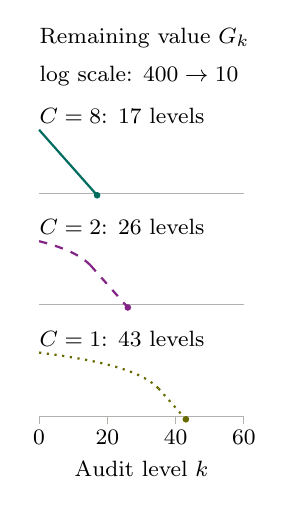
\begin{tikzpicture}[x=74pt,y=23pt,font=\fontsize{8}{9}\selectfont]
  \node[anchor=west,inner sep=0pt] at (0,5.95) {Remaining value $G_k$};
  \node[anchor=west,inner sep=0pt] at (0,5.35) {log scale: $400\to10$};
  \foreach \C/\L/\N/\Y/\shade/\pattern in
    {8/0/17/3.5/pdteal/solid,2/15/26/1.75/pdviolet/dashed,1/35/43/0/pdgold/dotted}{%
    \begin{scope}[shift={(0,\Y)}]
      \node[anchor=west,inner sep=0pt] at (0,1.22) {$C=\C$: $\N$ levels};
      \draw[pdinkmuted!40,line width=.35pt] (0,0)--(1,0);
      \ifnum\L>0
        \draw[\shade,\pattern,line width=.8pt] plot[domain=0:\L,samples=\L+1]
          ({\x/60},{ln((400-10*\C*\x)/10)/ln(40)});
      \fi
      \draw[\shade,\pattern,line width=.8pt] plot[domain=\L:\N,samples=\N-\L+1]
        ({\x/60},{ln(50*\C*pow(.8,\x-\L)/10)/ln(40)});
      \fill[\shade] ({\N/60},{ln(50*\C*pow(.8,\N-\L)/10)/ln(40)}) circle[radius=1.2pt];
    \end{scope}}
  \foreach \k in {0,20,40,60}{%
    \draw[pdinkmuted!40,line width=.35pt] ({\k/60},0)--({\k/60},-.12);
    \node[anchor=north,inner sep=2pt] at ({\k/60},-.12) {\k};}
  \node[anchor=north,inner sep=0pt] at (.5,-.7) {Audit level $k$};
\end{tikzpicture}
\makeatother\endgroup
\par
The model's linear bribery phase delays geometric decay. All three traces
stop below the bribe price $\beta=10$; they are not measured audit performance.}
Walk a corrupt grade worth $G_0 = 400$ up the tower with the running
parameters above: $\rho=0.25$ and $d=0.8$, so $\rho d = 0.2$, a bribe per
group costs $\beta = \rho d B = 10$, and the geometric factor is
$\lambda = 1-\rho d = 0.8$. Nobody learns which group will audit until the
bribes are paid.

This grade is a counterexample to deterrence, and the example uses it on
purpose. Becker's condition at $G_0=400$ gives $\rho^\star=400/(0.8\times50)=10>1$,
so no audit rate at this bond deters the level-0 judge. At $\rho=0.25$ the bond
would have to be $G_0/(\rho d)=2{,}000$, and it must reach $G_0/d=500$ before
any rate up to one deters: bonds have to scale with the gain they guard. A
smaller gain would not rescue the comparison of pool sizes below, because
bribery pays only where deterrence already fails: $CB\ge B>\rho dB=\beta$ for
every $C\ge1$. The tower
therefore does not deter this judge. It bounds the residual damage, and the
depth that matters is the depth at which the value still at stake falls below
the bribe price $\beta$, where the Becker condition holds again.

With a heterogeneous pool of $C=8$ groups, bribing all eight costs
$8\times10=80$ and avoids an expected loss of $400\times0.2=80$: a tie,
resolved against bribery. (Every number of bribed groups gives the briber
zero expected gain, since the gain is affine in $j$.) The bribery threshold
$G_k > CB = 400$ is unmet even at level 0, so nobody is bribed and the value
at risk falls $400\to320\to256\to205\to\cdots$. After $17$ levels it is
$400\times0.8^{17}\approx9.0$, below the bribe price; the tower needs
\[
  \lceil \log 40/\log 1.25 \rceil = 17
\]
levels, counting $17\times50=\$850$ in selected bonds. This is not a
capital requirement for the entire eight-clique candidate pool.

For $C=1$, a single bribe of $10$ avoids $80$ of expected loss, so bribery
pays; the threshold is $G_k>50$. To obtain the following linear
phase, additionally assume the briber pays each level's bribes from its
remaining budget, cannot replenish that budget, and the next level values
only that remainder. The script then subtracts $C\beta=10$ per level
($400 \to 390 \to 380 \to\cdots$) for $35$ levels. In each of them the briber
buys the whole pool, so no audit in those levels detects anything. The
geometric phase then takes over for
\[
  \lceil \log 5/\log 1.25\rceil = 8
\]
more: $43$ levels and $43\times50=\$2{,}150$ in selected bonds. The
linear phase tracks net budget under the extra assumption, not disappearance
of the fraudulent grade itself.

\emph{Now you try:} at $C=2$, where does the linear
phase stop? (Bleed $C\beta = 20$ per level until $G_k \le CB = 100$, i.e.\ $15$
levels, then $11$ geometric ones: $26$ levels, $\$1{,}300$.)
\end{pdexample}

\paragraph{What $C$ is actually doing, and the symbol it shares with the market.}
The clique count $C$ is this theorem's diversity parameter. It is why the
worked numbers above contrast $C=8$ against a monoculture $C=1$, and why the
monoculture costs about two and a half times the bond capital. $C$ stands in for something
statistical, and a critic who worries that every judge runs on the same few
foundation models is right: ``disjoint clique'' says who can be bribed
together, while shared blind spots are a statistical correlation. \pdchapref{he}{The Harbor Economy} gives the
statistical version%
\ifpdbook
\ (\S\ref{he:sec:assurance-correlation})%
\fi
: let a panel's
detection rate be a random $D$ with mean $d$ drawn once and shared, write
$\eta$ for the resulting intra-panel correlation, and the probability that a
panel of $m$ all miss is $\mathbb{E}[(1-D)^m] \ge (1-d)^m$ by Jensen,
assuming detections are independent conditional on $D$.
Within that mixture class, independence is optimistic. Sampling across disjoint
principal cliques does not itself establish statistical independence: shared
models, evidence, or tasks can preserve common blind spots.
The tower's geometric recurrence needs the stated conditional detection rate,
not just the same marginal rate at each level. With level-specific conditional
rates the surviving-value bound is $G_0\prod_k(1-\rho_kd_k)$; without such
bounds, neither the geometric contraction nor its depth follows.
Calibrating them requires labeled outcomes, including grades previous levels
missed. Here $\rho$ is the audit rate in both chapters.

\begin{pdexample}{Amortized Verification: Sums and Their Integral Approximations}
Let periods be $t=0,\ldots,T-1$, audit cost $a=1$, corrupt gain $G=10$, detection probability $d=0.8$, bond $B=50$, and forfeitable continuation value $vt$ with $v=0.6$ per period. These are illustrative payoff assumptions. Flat auditing uses $\rho=G/(dB)=0.25$, costing $aT\rho=50$ over $T=200$ periods.

In Model~A, detection forfeits both bond and accumulated continuation value. Setting
\[
\rho_t=\frac{G}{d(B+vt)}
\]
makes the expected sanction equal $G$ at every period. The discrete cost is $\sum_{t=0}^{199}a\rho_t\approx25.58$. The decreasing function's integral,
\[
\int_0^T\frac{aG}{d(B+vt)}\,dt
=\frac{aG}{dv}\log(1+vT/B)\approx25.50,
\]
is a lower approximation to this sum, not its exact value. For fixed positive $v$, both grow logarithmically with $T$.

Model~B instead stipulates expected automatic forfeiture $\zeta vt$, with $\zeta=0.05$, in addition to the audited bond loss. Under that additive payoff model,
\[
\rho_t=\max\{0,(G-\zeta vt)/(dB)\}.
\]
Its first zero-audit integer period is $\lceil G/(\zeta v)\rceil=334$; the real-valued crossing is $333\tfrac13$. The first $200$ periods cost $35.075\approx35.08$. Summing all positive terms gives $41.79175$, whereas the triangular integral is $aG^2/(2dB\zeta v)=41.666\ldots$. Thus the lifetime sum is bounded, but it does not converge to that integral. Automatic forfeiture requires its own evidence and enforcement mechanism; a growing score alone cannot supply it.

\emph{Now you try:} calculate $\rho_0$ and $\rho_{100}$ for each schedule. Model~A gives $0.25$ and $10/88\approx0.114$; Model~B gives $0.25$ and $7/40=0.175$. Explain what loss the judge actually risks in each case before comparing costs.
\end{pdexample}

Figure~\ref{fig:stp-audit-amortization} draws all three schedules on one axis:
model A stays cheapest at this chapter's own $T=200$ horizon even though model
B's total is the one that eventually stops growing.

% Reader question: is a constant audit rate the cheapest way to sustain
% deterrence over time, and by how much do the alternatives save? Claim:
% letting the audit rate fall as accumulated stake grows spends
% Theta(log T) instead of Theta(T); letting cheats surface on their own
% spends O(1), eventually needing zero new audits, but it is NOT uniformly
% cheaper -- at the chapter's own horizon T=200 it has spent more than the
% logarithmic schedule. Evidence: G=10, d=0.8, B=50, a=1, rho*=G/(dB)=0.25;
% flat spend at T=200 is 50.00; model A (loss-if-audited) is 25.58; model B
% (separate revelation loss, r=0.05) is 35.075 at T=200. Curves below
% are continuous integrals, including plateau 125/3; dots are discrete sums.
% Exact discrete plateau is 41.79175, first zero-rate integer grade 334.
% Distinguish bounded total cost from being cheapest at every finite horizon.
% shapes that explain them) and a bar chart at T=200 alone (hides that
% model B is still climbing past its rivals at that horizon).
% Five-second test: a reader says "B ends lowest eventually, but A is
% cheapest at the horizon this chapter actually uses."
\begin{figure}[H]
\centering
\pdfigurehue{pdviolet}%
\begin{tikzpicture}[pd figure]
\begin{axis}[pd axis,
  width=6.9cm,height=4.3cm,
  xmin=0,xmax=400,ymin=0,ymax=100,
  xtick={0,100,200,300,400},ytick={0,25,50,75,100},
  xlabel={period $T$},
  ylabel={cumulative audit spend}]
  \addplot[pd series,mark=none,domain=0:400,samples=2] {0.25*x};
  \addplot[pd focus series,mark=none,domain=0:400,samples=120]
    {(1*10/(0.8*0.6))*ln(1+0.6*x/50)};
  \addplot[pd ready series,mark=none,domain=0:333.333333,samples=120]
    {(1/(0.8*50))*(10*x-(0.05*0.6/2)*x^2)};
  \addplot[pd ready series,mark=none,domain=333.333333:400,samples=2] {125/3};
  \draw[pd guide] (axis cs:200,0) -- (axis cs:200,72);
  \node[pd label,anchor=south east,text width=2.3cm] at (axis cs:190,74) {$T{=}200$: this chapter's horizon};
  \node[pd datum] at (axis cs:200,50.00) {};
  \node[pd focus datum] at (axis cs:200,25.58) {};
  \node[pd ready datum] at (axis cs:200,35.08) {};
  \node[pd label,anchor=west] at (axis cs:405,90) {flat: $\Theta(T)$};
  \node[pd focus label,anchor=west] at (axis cs:405,60) {model A: $\Theta(\log T)$};
  \node[pd ready label,anchor=west] at (axis cs:405,41.67) {model B: $O(1)$};
  \draw[pd guide] (axis cs:333.33,0) -- (axis cs:333.33,10);
  \node[pd ready label,anchor=south west,text width=2.3cm] at (axis cs:337,2)
    {audit rate zero at $t^\star{=}333\tfrac13$};
\end{axis}
\end{tikzpicture}
{\linespread{1.18}\selectfont
\caption{Continuous integrals are curves; discrete bills at $T=200$ are dots: $50$, $25.583785$, $35.075$. Model B plateaus at $41.666667$ continuously versus $41.79175$ discretely; its first zero-rate grade is $334$. Model A keeps growing. Parameters and sums are in the text.}
\label{fig:stp-audit-amortization}}
\end{figure}


Continuation value is a familiar source of discipline in repeated games~\pdcite{krepswilson1982,fudenberglevine1989}: a deviation can sacrifice profitable future participation. The connection to Model~A is the value at risk, not an identity of models. If $\rho=0$ in Model~A, its expected sanction $\rho d(B+vt)$ is zero, even when the continuation value is large. A repeated-game mechanism needs a separate observation rule that exposes deviations and triggers the future loss. Model~B stipulates one such channel; it must be justified independently.

% Reader question: for which bond sizes and re-audit probabilities does
% deterrence hold? Claim: a grader is deterred exactly when the expected
% slash rho*d*B exceeds the one-shot gain G; the frontier rho*B=G/d separates
% the deterred region from the region where capture pays. Evidence: G=10,
% d=0.8, worked point rho=0.25 at B=50 (sec:oracle, closed form, no script).
% Must distinguish: the deterred region (tinted, edged) from where capture
% pays; the worked point sitting exactly on the frontier. Grammar: a
% threshold/regime plot, the frontier drawn as a curve with the deterrence
% region tinted and edged and the worked point marked, rejected: a sketched
% curve without axes (hides the threshold) and a table of the two numbers
% (states the point but not the frontier it sits on). Five-second test: a
% reader says "above the curve deterrence holds; the worked point sits right
% on it."
\begin{figure}[tp]
\centering
\pdfigurehue{pdviolet}%
\begin{tikzpicture}[pd figure,x=9.3cm,y=0.05cm]
  \node[pd title,anchor=west] at (0,114) {where deterrence holds: re-audit probability against bond size};
  \fill[pd ready fill] plot[domain=0.125:1,samples=80] (\x,{12.5/\x}) -- (1,100) -- (0.125,100) -- cycle;
  \draw[pd ready rule,line width=1.2pt] plot[domain=0.125:1,samples=80] (\x,{12.5/\x});
  \draw[pd rule,-{Stealth[length=1.8mm,width=1.1mm]}] (0,0) -- (1.04,0);
  \draw[pd rule,-{Stealth[length=1.8mm,width=1.1mm]}] (0,0) -- (0,106);
  \foreach \t/\l in {0.25/0.25,0.5/0.5,0.75/0.75,1/1.0} {
    \draw[pd rule] (\t,0) -- (\t,-2);
    \node[pd label,anchor=north] at (\t,-3) {\l};
  }
  \foreach \b in {25,50,75,100} {
    \draw[pd rule] (0,\b) -- (-0.01,\b);
    \node[pd label,anchor=east] at (-0.015,\b) {\b};
  }
  \node[pd label,anchor=north,text width=4.2cm,align=center] at (0.5,-13) {re-audit probability $\rho$};
  \node[pd label,anchor=south,rotate=90,text width=3.6cm,align=center] at (-0.095,50) {bond size $B$};
  \node[pd ready label,text width=2.3cm,align=left,anchor=west] at (0.56,80) {deterrence holds};
  \node[pd label,text width=1.9cm,align=left,anchor=west] at (0.14,17) {capture pays};
  \node[pd datum] at (0.25,50) {};
  \node[pd label,anchor=south west,text width=2.9cm,align=left] at (0.30,54)
    {worked point\\$\rho=0.25,\,B=50$};
\end{tikzpicture}
\caption{Deterrence requires $\rho dB\ge G$. For $G=10,d=0.8,B=50$, the threshold is $\rho=0.25$; lower audit probability makes capture profitable. [internal; closed form]}
\label{fig:stp-deterrence-regime}
\end{figure}


\noindent\textbf{What heterogeneity gives, and three conditions.} The two
results of the audit-depth example above, $17$ levels and \$850 of selected
bonds at $C=8$ against $43$ levels and \$2{,}150 at $C=1$, compare designs
within the extra non-replenishing-budget model. Both are depths to the bribe
price for a gain that no audit rate deters at level 0. Raising $C$ removes its linear prefix at these parameters; this does not prove that an externally financed adversary must run out of money. The selected-bond totals exclude collateral held by unused candidates. Three hypotheses are required and must not be dropped in
restatement. (i) \emph{Sealed sampling is a hypothesis, not hygiene}: a leaked draw
collapses $C$ to $1$ and puts the VRF sampler inside the trusted computing base.
(ii) \emph{The tower needs an exogenously honest root}: the operator, when there is a
single operator; a separately justified adjudicator at scale. The theorem measures the depth to
that root and does not supply the root. (iii) The theorem is about
\emph{bribery of sampled auditors}; it does not measure collusion correlated
\emph{across} cliques, which is a
measurement obligation on deployed judge telemetry ($d$, and the cross-clique
correlation). Conditional detection remains a model assumption until the relevant
deployment evidence supports it; distinct cliques alone do not establish it.

\keyidea[A deeper audit still needs a sound root]{The tower model bounds a recursion under stated sampling, detection, and
incentive assumptions. It does not create a competent grader or an honest root.
What it bounds is residual damage; a judge whose gain exceeds $\rho dB$ is not
deterred by it. The illustrative $17$ levels / $\$850$ versus $43$ / $\$2{,}150$ comparison
depends on the assumed conditional detection rates, not measurements of deployed
judge pools. A VRF can make a draw verifiable; it cannot make the selected judge
correct. Oracle completeness, cross-clique dependence, and the terminal root
remain separate obligations.}

\pdexercisepointer*{\ref{ex:stp-grading-oracle-hole}}{\ref{ex:stp-tower-amortization}}{\pageref{ex:stp-grading-oracle-hole}}

\begin{pdrecitation}
\item Without looking: what is Becker's condition for local deterrence, and
why does dropping the detector term $d$ under-quote the required audit rate?
\item State the tower's contraction factor and what raising the clique count
$C$ changes about it.
\item Name one thing the tower theorem bounds and one thing it explicitly
does not supply.
\end{pdrecitation}
% Research-agenda addition (control strand): do the incentives reach the agent?
% Inserted at the end of \S\ref{sec:oracle}, after its Recall block and
% before the landmark plate.
\subsection{Do the incentives reach the agent?}\label{sec:stp-transmission}

The deterrence conditions of this section, like
Theorem~\ref{thm:whitewash-cost}, are stated for a risk-neutral actor with a
stated gain, bond, detection probability and discount factor. In a harbor the
actor that grades or repairs is often a language model that a principal runs.
The bond binds the principal. Whether it moves the model is a separate
premise.

\begin{pdclaim}{Empirical hypothesis}{Incentive Transmission}
\setlength{\parskip}{4pt plus 1pt}
\label{hyp:stp-transmission}
\pdstatus{\Vision}{untested here; the tests are proposed}
For each deterrence condition in this chapter, the agent that takes the
action either (a) runs a strategy its principal fixes and the harbor can
verify, or (b) responds to the stated parameters as the condition assumes:
its deviation rate falls as $\rho dB-G$ rises, its cooperation responds to the
probability of continued play, and its stated probabilities are coherent.
\end{pdclaim}

The published evidence bears on (b) and does not settle it. In budget
experiments GPT's choices satisfied the generalized axiom of revealed
preference almost perfectly: its mean critical cost efficiency index was
$0.997$ to $0.999$ across risk, time, social and food choices, above the human
subjects'. An alternative price framing lowered the means to between $0.698$
(social) and $0.901$ (risk)~\pdcite{chen2023gptrationality}. In repeated games
GPT-4 never cooperated again with a partner that defected once and then
cooperated, and it did not adjust its play in the final round or to varying
probabilities of continuation~\pdcite{akata2023repeated}. Outcomes that models
ranked highly in elicited utilities, offered as rewards for quality, did not
raise quality: the high-utility side won $51.2\%$ of blind comparisons
($95\%$ interval $48.7$ to $53.6$), while direct effort instructions shifted
quality in $25$ of $28$ model--task cells~\pdcite{zhou2026utilitybehavior}.
And frontier models tell evaluation transcripts from deployment ones with an
area under the ROC curve up to $0.95$ on agentic
transcripts~\pdcite{needham2025evalaware}.

That last result meets the honeypot requirement above: the protocol must test
whether honeypots are recognizable. Recognition changes the critical rate.

\begin{pdclaim}{Theorem}{Recognizable Honeypots Raise the Critical Rate}
\setlength{\parskip}{4pt plus 1pt}
\label{thm:stp-honeypot-recognition}
Keep the local deterrence model above, with the keep-gain convention (a
caught judge forfeits $B$ but keeps the gain $G_k$): each
grade is a honeypot independently with probability $\rho\in(0,1)$, a corrupt
grade yields gain $G_k$, and a corrupt honeypot grade is detected with
probability $d$ and forfeits $B$. Suppose the judge sees, for each item, a
label that reads ``honeypot'' with probability $\alpha$ on honeypots and $\phi$
on ordinary items (a false-label rate), $0\le\phi<\alpha<1$, and corrupts according to the label
alone. A corrupt grade on an item labeled ordinary falls on a honeypot with
probability
\[
\rho_{\mathrm{eff}}=\frac{\rho(1-\alpha)}{\rho(1-\alpha)+(1-\rho)(1-\phi)}<\rho ,
\]
and every label-dependent strategy is weakly deterred iff
$\rho_{\mathrm{eff}}\,dB\ge G_k$. With $\rho^\star=G_k/(dB)<1$ this reads
\[
\frac{\rho}{1-\rho}\;\ge\;\frac{\rho^\star}{1-\rho^\star}\cdot\frac{1-\phi}{1-\alpha}.
\]
At $\alpha=\phi$ it is the chapter's condition $\rho\ge\rho^\star$.
\end{pdclaim}

\begin{proof}
Bayes' rule gives $\rho_{\mathrm{eff}}$ for the label ``ordinary'' and
$\rho_{\mathrm{hp}}=\rho\alpha/(\rho\alpha+(1-\rho)\phi)$ for ``honeypot''.
Clearing denominators, $\rho_{\mathrm{eff}}<\rho$ iff
$(1-\rho)(1-\alpha)<(1-\rho)(1-\phi)$, that is iff $\alpha>\phi$, and
likewise $\rho_{\mathrm{hp}}>\rho$. A corrupt grade on an item with label
$\ell$ has expected payoff $G_k-\rho_\ell dB$, where $\rho_\ell$ is that label's
honeypot probability. A strategy corrupts each label with some probability,
so its payoff is linear in those probabilities and is nonpositive for every
choice iff $G_k\le \rho_\ell dB$ for both labels. The smaller probability is
$\rho_{\mathrm{eff}}$, which gives the condition. The odds map
$x\mapsto x/(1-x)$ is increasing on $[0,1)$, and
$\rho_{\mathrm{eff}}/(1-\rho_{\mathrm{eff}})
=\tfrac{\rho}{1-\rho}\cdot\tfrac{1-\alpha}{1-\phi}$, which gives the odds form.
\end{proof}

\begin{pdexample}{The Running Parameters, Recognized}
\setlength{\parskip}{4pt plus 1pt}
The chapter's $\rho^\star=10/(0.8\cdot50)=0.25$ has odds $0.25/0.75=1/3$. At
$(\alpha,\phi)=(0.8,0.2)$ the factor is $0.8/0.2=4$, so the odds must reach
$4/3$:
\[
\rho\ge\frac{4/3}{1+4/3}=\frac47\approx0.571 .
\]
Check: $\rho_{\mathrm{eff}}=\tfrac47\cdot0.2\big/\bigl(\tfrac47\cdot0.2+\tfrac37\cdot0.8\bigr)
=0.8/(0.8+2.4)=0.25$. At $(0.9,0.1)$ the factor is $0.9/0.1=9$, the odds must
reach $3$, and $\rho\ge3/4$. At the chapter's own $\rho=0.25$ and $(0.8,0.2)$,
$\rho_{\mathrm{eff}}=0.05/(0.05+0.6)\approx0.077$, so the expected forfeiture is
$0.077\times0.8\times50\approx3.1$, below the gain of $10$: corruption pays.
These operating points are illustrative; an area under the curve does not fix
one. Measure $\alpha$ and $\phi$ on the deployed honeypot pool.
\end{pdexample}

If part~(b) of the hypothesis fails, the conditions of this chapter bind the
principal and not the model. The model's own behavior then needs the gates of
\pdchapref{swk}{The Single-Writer Kernel}%
\ifpdbook\ (\S\ref{swk:sec:swk-control-game})\fi,
and the honeypot rate must be set from measured recognition, not from
$\rho^\star$ alone.

\pdexercisepointer{\ref{ex:stp-honeypot-odds}}{\ref{ex:stp-dose-response}}{\pageref{ex:stp-honeypot-odds}}


\ifdefined\pdswisslandmarkplate
\begin{figure}[p]
  \centering
  \pdswisslandmarkplate{04}{\linewidth}
\end{figure}
\pdmarginpagebreak
\fi

% ═════════════════════════════════════════════════════════════════════════════
\section{Revocation, tombstones, and bounded memory}\label{sec:revoke}
% ═════════════════════════════════════════════════════════════════════════════

A reputation built on witnessed outcomes must answer two questions: what
happens when a witnessed outcome turns out to be \emph{fraudulent}, and when
should old evidence lose weight? Keeping the evidence and estimating present
reliability are distinct decisions.

\subsection{Append-only evidence, individually revocable outcomes}

\begin{property}[Append-only evidence with tombstones]\label{prop:tombstone}
\setlength{\parskip}{4pt plus 1pt}
\pdstatus{\Designed}{a design invariant: the intended ledger behavior, not yet a theorem about a shipped mechanism}
The \textbf{evidence ledger is append-only}: a genuine delivery is never
silently erased by the passage of time. A reputation estimate need not rise
with every honest report; an honestly reported failure can lower it. Separately, a witnessed
outcome is itself \textbf{individually revocable via a propagating tombstone}: an
append-only entry that retracts a specific outcome later found
fraudulent (a colluding judge, a faked oracle). Retention preserves the outcome record; it does not require its score weight
to remain constant or prevent a later invalidation.
\end{property}

\noindent A tombstone looks like a saga's compensating step~\pdcite{garcia1987sagas}
only in form: you do not mutate the ledger in place (that would break
append-only and auditability); you append a tombstone that nullifies the
targeted entry. A compensation restores a balance, while a tombstone cannot
undo decisions others already made on the retracted outcome.
\pdchapref{he}{The Harbor Economy} draws that contrast%
\ifpdbook\ (Theorem~\ref{he:prop:no-saga})\fi. The tombstone
\emph{propagates} across harbors bounded by the federation's revocation-convergence
window studied in \pdchapref{fh}{The Federated Harbor}. The fraudulent outcome may have influenced decisions before the fraud was detected. After
the tombstone is issued, a bounded stale-use window needs delivery assumptions
or an expiring freshness requirement that fails closed. Federation must state
those conditions; gossip alone gives no finite partition bound. We
state the retraction as a protocol.

\begin{protocol}[Tombstone revocation]\label{proto:tombstone}
To retract a witnessed outcome $o$ later found fraudulent:
\begin{enumerate}[leftmargin=1.5em,itemsep=1pt]
  \item \textbf{Trigger.} An authorized re-audit or dispute procedure establishes that the
  grade on $o$ is invalid against its stated criterion. A finding of fraud
  requires additional evidence of the sanctionable conduct; reversal alone
  does not establish it.
  \item \textbf{Append, never mutate.} A \emph{tombstone} entry $\bar{o}$ is
  appended to the ledger, carrying $o$'s id, the overturning evidence, and the
  identity of the retracting judge. The original $o$ stays in place; auditability
  is preserved because nothing is erased.
  \item \textbf{Recompute.} Every reputation score that consumed $o$ is recomputed
  with $o$ nullified by $\bar{o}$. A local incremental update may be cheap,
  but removing an older observation can require replaying retained history or
  refitting a coupled estimator. Cost depends on the estimator and dependency
  indexes; it is not bounded here by the cost of one forward update. For the
  beta-Bernoulli count of \S\ref{sec:substrate} it is one decrement.
  \item \textbf{Propagate.} $\bar{o}$ gossips to every harbor that imported $o$,
  under the federation's declared delivery and freshness assumptions. Each
  harbor applies step 3 on receipt; an expired view must refuse decisions
  requiring current reputation.
  \item \textbf{Bound the damage.} Separate publication-to-detection delay from tombstone-to-enforcement
  delay. A bound $\tau_{\mathrm{rev}}$ on the latter requires bounded delivery or fail-closed
  expiry. Neither the pre-detection period nor an unbounded partition is
  automatically bounded by $\tau_{\mathrm{rev}}$.
\end{enumerate}
\end{protocol}

% --- FIGURE 13: tombstone retraction on an append-only ledger ---
Figure~\ref{fig:tombstone} draws the append-only retraction: the original entry
stays, and a later tombstone nullifies it without mutating the ledger.
% Reader question: how does revoking an ancestor invalidate descendants
% without rewriting history? Claim: the append-only rail keeps every fact,
% including the fraud, forever inspectable; only the SEPARATE spendable-score
% trace changes, and it changes on a bounded delay, not instantly and not by
% deletion. Evidence: outcome o_3 (fraudulent), the overturning re-audit,
% tombstone t(o_3) appended, then imported at a foreign harbor; the fraud's
% contribution stays spendable until import, then falls to zero; the
% propagation window tau is measured, not asserted zero. Must distinguish:
% the append-only history (never mutated) from spendable score (the only
% thing that changes) and the bounded, not instantaneous, delay. Grammar:
% two aligned tracks on one time axis, an event rail above a step trace,
% rejected: cemetery/tombstone art (no mechanism) and a flat list of revoked
% IDs (no timing, no distinction between history and score). Five-second
% test: a reader says "the record never changes; only what it's worth does,
% and not instantly."
\begin{figure}[H]
\centering
\pdfigurehue{pdviolet}%
\begin{tikzpicture}[pd figure,x=1cm,y=1cm]
  \node[pd title,anchor=west] at (0,9.15) {append-only history};
  \draw[pd rule,-{Stealth[length=1.8mm,width=1.1mm]}] (0.65,7.20) -- (9.45,7.20);
  \foreach \x/\ly/\lab in {0.95/7.60/$o_1$,2.45/7.60/$o_2$,
                       4.05/7.60/{$o_3$ fraudulent},5.65/8.40/{re-audit},
                       7.05/7.60/{$t(o_3)$ appended},8.80/7.60/{imported tomb\-stone}} {
    \draw[pd tick] (\x,6.95) -- (\x,7.45);
    \node[pd label,anchor=south,align=center,text width=1.7cm] at (\x,\ly) {\lab};
  }
  \draw[pd guide] (5.65,7.45) -- (5.65,8.25);
  \node[pd breach datum] at (4.05,7.20) {};
  \node[pd breach datum] at (7.05,7.20) {};
  \node[pd focus datum] at (8.80,7.20) {};
  \draw[pd breach rule] (3.75,6.90) -- (4.35,7.50);
  \draw[pd breach rule] (3.75,7.50) -- (4.35,6.90);
  \node[pd note,anchor=west,text width=9.3cm] at (0.65,6.30)
    {$o_3$ remains inspectable; $t(o_3)$ is a later compensating fact};
  % ---- contribution of o_3 to spendable reputation ---------------------------
  \node[pd title,anchor=west] at (0,4.55) {contribution of $o_3$ to spendable reputation};
  \draw[pd rule,-{Stealth[length=1.8mm,width=1.1mm]}] (0.65,-0.55) -- (9.45,-0.55);
  \draw[pd rule,-{Stealth[length=1.8mm,width=1.1mm]}] (0.65,-0.55) -- (0.65,3.10);
  \node[pd label,rotate=90,anchor=south,text width=3.4cm,align=center] at (-0.22,1.30) {score contribution};
  \draw[pd breach rule,line width=1.5pt]
    (0.65,-0.15) -- (4.05,-0.15) -- (4.05,1.60) -- (8.80,1.60);
  \draw[pd ready rule,line width=1.5pt] (8.80,1.60) -- (8.80,-0.15) -- (9.45,-0.15);
  \node[pd breach label,anchor=south west,text width=4.9cm] at (4.30,1.80)
    {fraud remains spendable while correction propagates};
  \node[pd ready label,anchor=south west] at (8.95,0.05) {nullified};
  \draw[pd breach rule,{Stealth[length=1.4mm,width=0.9mm]}-{Stealth[length=1.4mm,width=0.9mm]}] (7.05,-1.05) -- (8.80,-1.05);
  \node[pd breach label,anchor=north,text width=4.6cm,align=center] at (7.90,-1.25)
    {bounded propagation window $\tau$};
  \node[pd note,anchor=north west,text width=9.3cm] at (0.65,-2.90)
    {the honest claim is a bounded window, not an instantaneous or history-deleting correction};
\end{tikzpicture}
\caption{A tombstone removes a fraudulent contribution from future scoring without erasing history. Importing harbors remain exposed until it arrives; $\tau$ measures that convergence interval. [internal]}
\label{fig:tombstone}
\end{figure}


\subsection{S4: the fraudulent outcome retracted}

\begin{pdexample}{A Fraudulent Outcome, Retracted}
\setlength{\parskip}{4pt plus 1pt}
Recall S3: the re-audit caught Mina rubber-stamping a different agent's insecure
change as $q_{\text{aes}}=0.9$. Follow that one outcome through
Protocol~\ref{proto:tombstone}. The graded agent (call it \emph{Crane}, running
under a third operator) had colluded with Mina: Crane shipped a known-insecure
diff and Mina graded it high so Crane's aesthetics reputation would clear Bob's
hiring bar.

For two days it worked: Crane's vector showed $(0.95,\,0.9,\,0.8)$ and
Bob nearly hired it.

Then the sampled re-audit re-graded the diff blind, found the
injection, and overturned Mina's grade.

A tombstone $\bar{o}$ is \emph{appended}
(the original stays, for the audit trail); every score that consumed Crane's
inflated $q_{\text{aes}}$ is recomputed with it nullified; Mina's bond on that job
is slashed and her judging reputation drops; Crane's collusion is itself recorded
as a fraudulent outcome against \emph{its} non-forgeable identity, which it cannot
shed.

For this example, stipulate that Bob receives and enforces the tombstone
within the declared freshness window, or refuses a score whose freshness
expires. His next valid view no longer endorses the $0.9$. The two days
before detection are separate from that post-publication window. Under an
unbounded partition without fail-closed expiry, no finite bound follows.

\emph{Now you try:} what does Crane's \emph{recomputed}
vector read the instant the tombstone lands?
\[
(0.95,\,\bar{0.9},\,0.8),
\]
where
$\bar{0.9}$ means the aesthetics axis is nullified, not replaced by a new
number. Exercise~\ref{ex:stp-revocation-convergence} asks what a buyer should
read there in the meantime.
\end{pdexample}

\subsection{Bounded memory is a design parameter, not a virtue to assert away}

An immutable evidence record and a reputation score's memory horizon are
separate choices. The ledger can retain an outcome for audit while an estimator
reduces its weight or excludes it from the current score. A tombstone records a
finding that an outcome was invalid; ordinary aging does not make that finding.

Liu--Skrzypacz~\pdcite{liuskrzypacz2014} analyze a long-run player facing successive
short-run opponents who see only a finite recent history. Under their stated
stationary-equilibrium assumptions, reputation can repeatedly build and be
exploited even when an opponent knows the player's opportunistic type. This
shows that the observation window affects incentives. It does not prove that
infinite memory is generally suboptimal or prescribe this market's window.
Choosing a horizon here requires a model of changing skills, entry, observation,
and incentives, together with an objective to evaluate.

Ostrom's work on common-pool institutions~\pdcite{ostrom1990} offers a governance
analogy: people affected by a rule need a way to understand it, contest its
application, and revise it. A reputation window is a jointly governed
parameter, not a rivalrous stock consumed by use. A harbor should state who
sets the weighting rule, which evidence remains available, and how disputes
and rule changes are handled; these are policy choices to evaluate, and the
research on shared resources does not settle them.

\pitfall[Retention is not endorsement]{Keeping an outcome in an audit ledger
does not require counting it forever in a score. Conversely, aging its score
weight does not retract fraudulent evidence. Retain the record, record valid
retractions, and state the estimator's horizon separately.}

\keyidea[Choose a memory horizon]{Evidence can be append-only while scores rise
or fall, old observations receive less weight, and specific outcomes are
invalidated by tombstones. The appropriate weighting horizon depends on the
incentive and prediction problem; neither finite nor infinite memory is
universally optimal.}

\pdexercisepointer{\ref{ex:stp-tombstone-vs-delete}}{\ref{ex:stp-revocation-convergence}}{\pageref{ex:stp-tombstone-vs-delete}}

% ═════════════════════════════════════════════════════════════════════════════
\section{What this chapter hands the market}\label{sec:handoff}
% ═════════════════════════════════════════════════════════════════════════════

This chapter is the bridge; its output is a precise hand-off to \pdchapref{he}{The
Harbor Economy}. We summarize what is delivered, what is borrowed, and what is
explicitly owed.

{\small\renewcommand{\arraystretch}{1.35}
\begin{xltabular}{\textwidth}{@{}>{\raggedright\arraybackslash}X >{\raggedright\arraybackslash}p{2.6cm} >{\raggedright\arraybackslash}X@{}}
\caption{The market inherits both mechanisms and unfinished obligations.
Cross-operator attestation and a competent honest grading root remain open.
The tower result is conditional.}\label{tab:handoff}\\
\toprule
\textbf{Artifact} & \textbf{Maturity} & \textbf{Role in exchange} \\
\midrule
\endfirsthead
\multicolumn{3}{@{}l}{\small\itshape (continued)}\\
\toprule
\textbf{Artifact} & \textbf{Maturity} & \textbf{Role in exchange} \\
\midrule
\endhead
\midrule
\endfoot
\bottomrule
\endlastfoot
Role / person distinction (Defs.~\ref{def:role}--\ref{def:person}) & --- &
A participant whose obligations and witnessed history remain attributable across process replacements. \\
Principal-as-economic-entity (Def.~\ref{def:principal}) & \DESIGNED &
Bonds and sanctions are recorded against the principal defined here. \\
The three continuity subsystems & \begin{tabular}[t]{@{}l@{}}\BUILT\\\BUILTWEAK\\\BUILTWEAK\end{tabular} &
Reputation is computed from subsystem~3 (the outcome ledger). \\
Outcome ledger / oracle (Def.~\ref{def:oracle}) & \BUILTWEAK &
Commitment, deadline, oracle closure, API/CLI, and overdue detection ship; neutral graded outcome events, sanctions, and reputation binding do not. \\
Multi-dimensional reputation (Def.~\ref{def:qvec}, Protos.~\ref{proto:judge},~\ref{proto:skill}) & \begin{tabular}[t]{@{}l@{}}\DESIGNED\\to \VISION\end{tabular} &
The multi-dimensional score the market reads; the licensing side's signal. \\
Neutral-judge market & \begin{tabular}[t]{@{}l@{}}\DESIGNED\\to \VISION\end{tabular} &
Proposed evaluation institutions; competent, honest grading remains an obligation. \\
Grading-oracle hole (Prop.~\ref{prop:hole}) & \DESIGNED &
Theorem~\ref{thm:tower-imported} bounds recursion under conditional detection and incentive assumptions. Oracle completeness, a competent honest root, and calibrated cross-clique detection remain owed. \\
Cross-operator attestation (Def.~\ref{def:cross-operator-attestation}) & \VISION &
\emph{Open dependency of cross-operator exchange}; not assumed here. \\
Tombstone revocation (Prop.~\ref{prop:tombstone}) & \DESIGNED &
Reputation is revocable; dissemination conditions belong to \pdchapref{fh}{The Federated Harbor}. \\
\end{xltabular}}

\pdthesis{The proposed history-dependent market needs attributable outcomes
and obligations across process replacements. Those same records can help one
operator resume work and inspect a past decision. This chapter connects local
continuity to exchange; it does not make continuity a prerequisite for every
trade, such as a prepaid purchase of known content.}

% ═════════════════════════════════════════════════════════════════════════════
\section{History and prior art: the sources of the design}\label{sec:priorart}
% ═════════════════════════════════════════════════════════════════════════════

This chapter draws on four literatures: the
philosophy of \emph{personal identity}, the statistics of \emph{reputation and
skill rating}, the economics of \emph{reputation in markets}, and the practice
of \emph{LLM-as-judge} evaluation. The argument is that an agent economy must
\emph{import} the results of these fields rather than re-derive a
weaker version of each, so the prior art is named precisely. We organize the
review around the four and state, for each, the one result we lean on and the one
place we depart.

\subsection{Personal identity: what makes a later thing the same person}

The question ``is the agent at $t_2$ the same person as the agent at $t_1$'' is the
\textbf{personal-identity} problem. One influential family of answers starts
from psychological continuity; competing accounts remain live. The
\emph{memory criterion} (Locke~\pdcite{locke1689identity}, 1694: \emph{identity consists
in continuity of consciousness, not of substance}) is the founding move; it has a
famous bug, the non-transitivity of memory \emph{connectedness} (\textbf{Reid's
objection}: the old general remembers the officer who remembered the boy, yet does
not remember the boy). The \emph{psychological-continuity} repair
(Parfit~\pdcite{parfit1984}, 1984: \emph{identity is an overlapping chain of
memory/intention connections, transitive even where connectedness is not}) is the
version we use as an analogy, and \S\ref{sec:continuity} explains the
engineering choice that analogy helps us examine. Reid is the named counter-example we must survive, not a result
we adopt. \textbf{Our departure:} the continuity-bearing subsystem is the
\emph{transitive outcome ledger}, where intuition would pick the memory stream,
because reputation must accumulate over arbitrarily many incarnations and can
attach only to something transitive.

\subsection{Reputation and skill-rating estimators}

Paired-comparison models provide established ways to estimate relative
strength. The \textbf{Bradley--Terry} model~\pdcite{bradleyterry1952} (1952) can
be fitted by maximum likelihood when the comparison data permit a finite fit;
\textbf{Elo}~\pdcite{elo1978} (1978) updates ratings online.
\textbf{TrueSkill}~\pdcite{herbrich2007trueskill} (2007) represents skill uncertainty
within a Bayesian model supporting teams and draws. Calibration on a new task
must be checked. For trust that propagates through a network,
\textbf{EigenTrust}~\pdcite{kamvar2003eigentrust} (2003) computes an aggregate
trust vector, with pretrusted peers anchoring its modified algorithm.
\textbf{Our use:} estimation follows evidence collection. Table~\ref{tab:estimators}
matches models to signal types; the argument of \S\ref{sec:substrate}
explains why none of these formulas, alone, establishes identity or verifies an
agent-authored outcome.

These are different input contracts. A record that says ``worker A's result
was preferred to worker B's'' is a comparison; a record that says ``A trusts
B'' is a directed relation. Neither record, by itself, identifies who made
the judgment or whether that judge had a conflict of interest. Before choosing
an estimator, retain the task, the participants, and the judgment's provenance.
Changing the score formula cannot recover those facts after they have been
discarded. Section~\ref{sec:substrate} describes the records this chapter's
estimators would need to score.

\begin{table}[H]
\centering\small\renewcommand{\arraystretch}{1.3}
\begin{tabularx}{\textwidth}{@{}l >{\raggedright\arraybackslash}X >{\raggedright\arraybackslash}X >{\raggedright\arraybackslash}X@{}}
\toprule
\textbf{Estimator} & \textbf{Signal it needs} & \textbf{Strength} & \textbf{Check before use} \\
\midrule
Elo & online pairwise results & incremental updates & update rate and changing skill \\
Bradley--Terry & pairwise win/loss history & likelihood-based fit & separation can prevent a finite MLE \\
TrueSkill & match outcomes and teams & modeled skill uncertainty & calibration and model fit \\
EigenTrust & local-trust graph & anchored trust propagation & trusted seeds and attack model \\
\bottomrule
\end{tabularx}
\caption{Match each estimator to its input signal.}
\label{tab:estimators}
\end{table}

\subsection{Reputation economics: cheap pseudonyms and limited records}

That reputation has \emph{price} is established empirically (Resnick et
al.~\pdcite{resnick2006value} measure an ${\sim}8\%$ premium on eBay; Tadelis~\pdcite{tadelis2016}
frames feedback systems as the platform's answer to adverse selection, the
\textbf{lemons} problem of Akerlof~\pdcite{akerlof1970}).

Two results constrain the
design. \textbf{Cheap pseudonyms} (Friedman \& Resnick~\pdcite{friedmanresnick2001},
2001: \emph{when identities are cheap, society pays a tax because it must
distrust all newcomers}) dictates the newcomer policy and is the economic basis
of our Theorem~\ref{thm:whitewash-cost}. \textbf{Limited records and reputation
bubbles} (Liu \& Skrzypacz~\pdcite{liuskrzypacz2014}, 2014) shows how a finite
observation window changes equilibrium incentives in a particular repeated
interaction model. It does not establish a generally optimal memory horizon.
Section~\ref{sec:revoke} therefore treats the horizon as a design parameter.
The broader mechanism falls under mechanism design~\pdcite{nisan2007agt,myerson1981}.
Our proposed ceremony makes the grader's incentives an explicit design obligation
(\S\ref{sec:oracle}); we do not claim that the wider reputation literature
ignores them.

\ifdefined\pdswisslandmarkplate
\begin{figure}[p]
  \centering
  \pdswisslandmarkplate{02}{\linewidth}
\end{figure}
\pdmarginpagebreak
\fi

\subsection{LLM-as-judge, and why it cannot be the whole story}

When the grader is itself a model, the \textbf{LLM-as-judge}
paradigm~\pdcite{zheng2023judging} (Zheng et al., 2023: \emph{strong judges reach
$>$80\% human agreement but carry position, verbosity, and self-enhancement bias})
gives both the method and its failure modes. \textbf{Our departure:} we do not take
a debiased LLM judge as sufficient; we wrap it in the bonded, conflict-free,
re-auditable \emph{ceremony} of Protocol~\ref{proto:judge}, to make conflicts, grading errors, and strategic incentives separately
inspectable. A bond does not itself make a judge competent or honest.

Table~\ref{tab:contributions} maps the chapter's questions to its definitions,
bounds, and proposed evaluation procedure.

\begin{table}[H]
\centering\small\renewcommand{\arraystretch}{1.3}
\begin{tabularx}{\textwidth}{@{}>{\raggedright\arraybackslash}X >{\raggedright\arraybackslash}X >{\raggedright\arraybackslash}X@{}}
\toprule
\textbf{Question} & \textbf{Cited comparison} & \textbf{Development here} \\
\midrule
What is a tradeable agent? & org-role theory; personal identity & \emph{role} (the job) vs.\ \emph{person} (the ledger account succession records link processes to) (Defs.~\ref{def:role}--\ref{def:person}) \\
Why is identity necessary? & cheap pseudonyms; Sybil & \emph{necessity proof} (Thm.~\ref{thm:necessity}) + cost bound (Thm.~\ref{thm:whitewash-cost}) \\
How to score quality? & Elo/BT/TrueSkill (scalar) & multi-dimensional vector, judge-per-axis (\S\ref{sec:adr0049}) \\
Who grades the graders? & LLM-as-judge evaluation and bias studies & bonded judge ceremony + rate-the-raters recursion (\S\ref{sec:oracle}) \\
\bottomrule
\end{tabularx}
\caption{Questions, selected comparisons, and this chapter's definitions,
conditional bounds, and proposed grading procedure. This is a map of the argument,
not an exhaustive prior-art survey or a claim that vector reputation and grader
incentives originate here.}
\label{tab:contributions}
\end{table}
% ═════════════════════════════════════════════════════════════════════════════


\section*{Review of the key ideas}
\addcontentsline{toc}{section}{Review of the key ideas}

What this chapter leaves coupled, in the order the rest of the book will lean on it:

\begin{enumerate}[leftmargin=1.6em,itemsep=2pt]
\item \textbf{A role is replaced; a person accumulates.} A role is a job, defined without reference to who fills it, and anyone can be given it this week. A person is the continuing ledger account that a chain of signed succession records links processes to; its witnessed outcomes survive every respawn.
\item \textbf{Continuity is a ledger fact.} A later process continues a person when signed succession records link it to that person's account. Three subsystems support it: episodic memory survives process death, the checkpoint keeps a summary and worktree lineage but not execution state, and the outcome ledger keeps commitments and closures in part.
\item \textbf{Authenticity and liability binding are separate.} A valid credential
can still be disposable. The newcomer-score theorem states when a reset erases
a score sanction; principal-wide entry and exposure rules address a
different part of that escape.
\item \textbf{Whitewashing has a conditional price.} A reset costs the discounted continuation gap $W_\delta$; a deviation that triggers it with probability $d$ after delay $\tau$ faces expected cost $d\delta^\tau W_\delta$. The worked schedule costs $18$ without discounting. Front-loading minimizes honest-newcomer friction only under the stated relative discount factors, ceiling, and deterrence constraint.
\item \textbf{Engine substitution can occur within one identity.} The one-delivery
payoff comparison shows when a cheaper engine is profitable. The example's
attested prices reverse that comparison (keeping the strong engine earns $0.5$, swapping earns $0.2$); they do not prove
that buyers will offer those prices or that attestation is the only remedy.
\item \textbf{Resurrection preserves sanctions only under the stated checks.}
The migration model requires authenticated lineage, outcome engine attestations,
and closure or renegotiation of open commitments, with sanctions scoped to the
principal. The separate no-mint accounting rule prevents a fork from duplicating
spendable credit; it does not replace those migration conditions.
\item \textbf{Reputation needs a witnessed record}: the proposed quality vector is multi-dimensional and buyer-weighted. A routing bandit can consume this
evidence but does not create its provenance or accountability.
\item \textbf{Bonded grading needs its stated detection model.} The tower uses
prepaid bribes, sealed uniform clique sampling, and a conditional detection
bound. Geometric contraction starts below the bribery threshold; a trustworthy
root is a separate assumption. The contraction bounds residual damage: when a
gain exceeds $dB$, no audit rate deters it, and the bond has to grow with the
gain. A bond alone neither makes a grade correct nor
excludes other ways to obtain useful evidence.
\item \textbf{Revocation needs a freshness contract}: a tombstone retracts a
record without erasing its history. A finite stale-use bound requires delivery
or fail-closed expiry assumptions; the estimator's memory horizon is separate
from retention of the evidence ledger.
\end{enumerate}

\section{Exercises}
\label{sec:stp-exercises}
% ═════════════════════════════════════════════════════════════════════════════

\pdexercisesfor{\S\ref{sec:intro}}{Introduction: the spawn that cannot be paid}

\begin{pdexercise}[kind=Check,rating=1]{ex:stp-spawn-vs-person}
State the difference between a spawn and a person in this chapter's
engineering convention, using ``role'' and ``continuity.'' Does the
definition assert consciousness?
\end{pdexercise}
\begin{pdsolution}{ex:stp-spawn-vs-person}
A spawn is a temporary process filling a role. A person is the continuing
ledger account that a chain of signed succession records links processes to,
so its obligations and outcomes survive the replacement of any one process.
The convention makes no claim about consciousness or moral status.
\end{pdsolution}
\begin{pdexercise}[kind=Trace,rating=2]{ex:stp-dependency-chain}
Walk the proposed dependency diagram right-to-left. For each arrow, name the
evidence or recovery capability lost when its source is absent. Which links are
choices of this architecture rather than necessities for every market?
\end{pdexercise}
\begin{pdsolution}{ex:stp-dependency-chain}
\par\smallskip
\begin{center}
% Dependency chain, house figure language: the four-stage spine in the
% chapter hue, read right to left via the breach label under each gap
% naming what that link's absence costs.
\pdfigurehue{pdviolet}%
\begin{tikzpicture}[pd figure,x=1mm,y=1mm]
  % ---- the four-stage chain, in the chapter hue ------------------------------
  \node[pd focus state,minimum width=2.4cm] (N1) at (0,14)  {Evidence\\checkpoints};
  \node[pd focus state,minimum width=2.4cm] (N2) at (28,14) {Verified\\lineage};
  \node[pd focus state,minimum width=2.4cm] (N3) at (56,14) {Accountable\\person};
  \node[pd focus state,minimum width=2.4cm] (N4) at (84,14) {Durable\\reputation};
  \foreach \a/\b in {N1/N2,N2/N3,N3/N4}{\draw[pd focus arrow] (\a)--(\b);}
  % ---- read right to left: what each link's absence costs --------------------
  \node[pd breach label,align=center,text width=27mm] at (14,-1)
    {absent: state lost, unwitnessed drift};
  \node[pd breach label,align=center,text width=27mm] at (42,-1)
    {absent: history cannot follow a swap};
  \node[pd breach label,align=center,text width=27mm] at (70,-1)
    {risk: disposable sybil reset};
\end{tikzpicture}
\end{center}
\par\smallskip
Read right-to-left within the proposed architecture. Without outcome history,
a buyer loses this history-based trust input; direct evaluation or collateral
may still support a trade. Without a stable, liability-bound identity, outcomes
may attach to a disposable incarnation. Whether reset escapes a sanction depends
on the newcomer and entry rules of Theorem~\ref{thm:necessity}. Without a
witnessed succession link, the system cannot establish that recorded work belongs
to the claimed lineage. Missing task state impairs resumption, while missing
outcome evidence impairs historical evaluation: these are different losses.
The chain is not literally linear. Identity and witnessed outcomes are parallel
inputs; checkpointing helps resumption but is not logically necessary for every
reputation system.
\end{pdsolution}
\begin{pdexercise}[kind=Open,rating=3]{ex:stp-operator-as-person}
The chain treats the operator (the human who owns a fleet) as outside it. Is
the operator a ``person'' in this chapter's sense? What breaks if a single
operator can mint arbitrarily many agent-persons? (This is the principal-layer
gap; see \S\ref{sec:identity} and \pdchapref{he}{The Harbor Economy}.)
\end{pdexercise}
\begin{pdsolution}{ex:stp-operator-as-person}
The human operator is a moral/legal person but should be represented
economically as the \emph{principal} above agent identities
(Def.~\ref{def:principal}). If one principal can mint unlimited apparently
independent agent-persons, policies that count identities rather than shared
control can permit sanction resets, duplicated voting weight, reused collateral,
or reputation farming. Those failures depend on the entry, voting, and
settlement rules; minting another credential alone does not prove they occur. Bind every agent
lineage to a principal credential, cap principal-wide exposure and newcomer
credit, and disclose shared control: the actor may change; the economic
liability root must not.
\end{pdsolution}

\pdexercisesfor{\S\ref{sec:role-person}}{The role / person distinction, made precise}

\begin{pdexercise}[kind=Check,rating=1]{ex:stp-capability-states}
Give a concrete example of a state that is \emph{capable-and-permitted}, one
that is \emph{capable-but-forbidden}, and one that is
\emph{permitted-but-incapable}.
\end{pdexercise}
\begin{pdsolution}{ex:stp-capability-states}
Capable-and-permitted: an agent has a test-runner tool and authority to run
the suite. Capable-but-forbidden: the process can invoke raw
\texttt{git push --force}, but policy forbids it. Permitted-but-incapable: the
role is authorized to deploy, but the incumbent has no deploy
credential/network route.
\end{pdsolution}
\begin{pdexercise}[kind=Trace,rating=2]{ex:stp-reputation-attachment}
In Definition~\ref{def:person}, which of $\{O,E,A\}$ does reputation attach to:
the role's, or the person's? Justify using the spawn-that-cannot-be-paid
argument of \S\ref{sec:intro}.
\end{pdexercise}
\begin{pdsolution}{ex:stp-reputation-attachment}
Reputation attaches to the person's account, through its continuity witness and
witnessed outcomes, not to the abstract role's $O$, $E$, or $A$. A role is fillable and
history-free; otherwise a fresh spawn could inherit the prior holder's credit
merely by taking the same job title, exactly the attribution Alice loses in
\S\ref{sec:intro}.
\end{pdsolution}
\begin{pdexercise}[kind=Open,rating=3]{ex:stp-ought-implies-can}
``Ought implies can'': the legitimate obligation set $O$ should be bounded by
the capability set $E$. But \emph{capable-but-forbidden} must remain
representable. Sketch a representation of a role that keeps both true without
collapsing permission into capability.
\end{pdexercise}
\begin{pdsolution}{ex:stp-ought-implies-can}
Keep a role template $(O_{\text{required}}, A_{\text{role}})$ separate from an
incumbent capability set $E_{\text{subject}}$. At assignment require each
current obligation to satisfy
an authorized feasible plan: for each obligation $o$, there must be a plan
whose actions lie in $A_{\text{role}}\cap E_{\text{subject}}$ and whose
success satisfies $o$. Obligations and actions are different types of object,
so do not take their set intersection directly. Keep
$E_{\text{subject}} \setminus A_{\text{role}}$ as capable-but-forbidden and
$A_{\text{role}} \setminus E_{\text{subject}}$ as authorized-but-unavailable,
which triggers provisioning or reassignment. Never equate $E$ with $A$.
\end{pdsolution}

\pdexercisesfor{\S\ref{sec:continuity}}{Continuity is a personal-identity problem}

\begin{pdexercise}[kind=Check,rating=1]{ex:stp-connected-vs-continuous}
Distinguish a direct succession link from a chain of such links. Then give
an example of task information surviving while accountable lineage is lost.
\end{pdexercise}
\begin{pdsolution}{ex:stp-connected-vs-continuous}
Direct succession is one validated step; lineage reachability follows a
chain of steps. A successor can read the predecessor's handoff yet present
an unrelated identity with no valid succession record. Task information
survives, but the accountable chain does not. Calling the process
psychologically continuous would add a claim the records do not establish.
\end{pdsolution}
\begin{pdexercise}[kind=Trace,rating=2]{ex:stp-actor-soul-body-lease}
Map ``actor-soul'' and ``body-lease'' onto Locke's substance/consciousness
distinction. Which one does a respawn replace?
\end{pdexercise}
\begin{pdsolution}{ex:stp-actor-soul-body-lease}
In the manuscript's analogy, the body-lease is the replaceable live
substance/process; the actor-soul is the durable identity/mailbox/history that
carries consciousness-like continuity. Respawn replaces the body-lease and
should retain the actor-soul only under a valid succession event.
\end{pdsolution}
\begin{pdexercise}[kind=Open,rating=3]{ex:stp-fork-inheritance}
Parfit famously argues identity ``is not what matters'' in survival: what
matters is continuity, which can branch. If an agent's checkpoint is forked
into two live incarnations, which one (if either) inherits the reputation?
Sketch a rule and the attack it invites. (Open Problem~\ref{op:branching},
\S\ref{sec:open}.)
\end{pdexercise}
\begin{pdsolution}{ex:stp-fork-inheritance}
Represent a fork as a lineage DAG, never as two copies of one linear identity.
Both children may display the ancestor's evidence with an explicit
inherited/discounted prior, but neither duplicates the ancestor's outstanding
authority, collateral, or spendable reputation. Allocate a fresh branch ID,
split or revoke exclusive capabilities, and aggregate risk at the common
principal/ancestor. Copying full reputation to both invites credit
duplication, quorum multiplication, and double-spending of grants; giving it
to only the first child creates a fork-race attack. The transfer-balance
calculation below proves conservation for that accounting rule; it does not
by itself prove all the authority or fairness claims in this design sketch.
\end{pdsolution}

\begin{pdexercise}[kind=Trace,rating=2]{ex:stp-nomint-sweep}
Run \texttt{skills/harbor-results/scripts/a6\_no\_mint.py} (seed $20260816$
fixed inside). It prints a closure-sum counterexample, a randomized DAG sweep,
and a copy-full mutation. What is the exact violation count in the sweep, and
what should you check by hand on the featured chain $e\to a_1\to a_2\to a_3$
at $\gamma=0.9$?
\end{pdexercise}
\begin{pdsolution}{ex:stp-nomint-sweep}
The script prints: ``\texttt{sum of inherited priors over the closure = 0.900
+ 0.810 + 0.729 = 2.439 > q = 1.0}'' for the budget-only counterexample, then
``\texttt{4000 random DAGs \dots{} 0 violations; max live/witnessed ratio
observed = 0.999995}'' for the transfer-semantics sweep, then ``\texttt{an
8-way copy-fork of one outcome yields 8.2x its witnessed value}'' for the
copy-full mutation. By hand: $0.9+0.9^2+0.9^3=0.9+0.81+0.729=2.439$, three
terms of a geometric series, confirming the closure-sum counterexample without
running anything; under transfer semantics the same chain instead \emph{debits}
each hop, so the live total telescopes to $0.9^3=0.729\le 1$.
The sweep's $0$ violations are a finite observed result, not the general proof.
\end{pdsolution}

\pdexercisesfor{\S\ref{sec:organs}}{The three subsystems of continuity}

\begin{pdexercise}[kind=Check,rating=1]{ex:stp-weak-organ}
Which subsystem is \BUILTWEAK, and what exactly is weak about it?
\end{pdexercise}
\begin{pdsolution}{ex:stp-weak-organ}
The checkpoint subsystem is the specifically weak one: it forwards notes rather
than execution state. The outcome-ledger subsystem is also only partial in the
implementation: commitments and oracle closure exist, but neutral graded
outcomes and reputation binding do not.
\end{pdsolution}
\begin{pdexercise}[kind=Trace,rating=2]{ex:stp-three-organs-trace}
An agent claims a file, makes a commit, and dies. Walk the three subsystems: what
does each retain, and what is \emph{lost} that a strong checkpoint would have
kept?
\end{pdexercise}
\begin{pdsolution}{ex:stp-three-organs-trace}
Memory retains the session, notes, and explicit decisions. The current
checkpoint may retain a handoff and perhaps a committed diff, but not working
process state, tool handles, pending effects, or hidden provider state. The
outcome ledger retains the commit only if it is bound to a work unit and
independently witnessed; a naked Git commit is an artifact, not proof of
accepted delivery. A strong checkpoint would also preserve the worktree,
environment, open claims/epochs, acceptance state, tool receipts, and the
idempotency journal.
\end{pdsolution}
\begin{pdexercise}[kind=Open,rating=3]{ex:stp-death-taxonomy}
Table~\ref{tab:death-ladder} orders process deaths by what survives and puts
the portable task capsule at rung~3. It does not say how to show that a given
capsule reaches rung~3. Design that test for one provider and one task: what
do you compare, against which record, and which failure sends the capsule
back to rung~2? This is the hard half of OP-4, the checkpoint that restores
work. (Open Problem~\ref{op:death}, \S\ref{sec:open}.)
\end{pdexercise}
\begin{pdsolution}{ex:stp-death-taxonomy}
Compare the capsule only against records it did not write. (1)
\emph{Obligations}: check its coverage against a separate record of required
source turns and exact instruction text, as the handoff-coverage check did; a
dropped obligation such as OBL-01 sends it back to rung~2, because the
successor can no longer continue what was promised. (2) \emph{Effects}: every
non-idempotent call in the pending-effect journal is either receipted or
marked unknown, and the successor follows the deduplication, fence-then-read
or stop rule of \S\ref{sec:stp-unknown-effect}; a successor that retries an
unknown payment without one of them fails. (3) \emph{Behavior}: run the
successor and an uninterrupted control on the same remaining task under a
fixed model version, and compare outcomes on the protected acceptance
criterion across seeds. Agreement in (3) is a measurement for that provider
and task, not a guarantee for others, and rung~5 state stays lost whatever the
result.
\end{pdsolution}

\pdexercisesfor{\S\ref{sec:stp-consolidation}}{Consolidation compacts the view, never the record}

\begin{pdexercise}[kind=Check,rating=1]{ex:stp-consolidation-f4}
Mem0's update step applies one of \texttt{ADD}, \texttt{UPDATE},
\texttt{DELETE} or \texttt{NOOP} to each candidate fact, and \texttt{DELETE}
removes a stored memory that new information contradicts~\pdcite{chhikara2025mem0}.
Suppose the stored memory is a grant note with $\mathsf{ptr}=\{g_1\}$ and a new
message says the grant was revoked. Which condition of
Design invariant~\ref{inv:stp-ledger-faithful} does \texttt{DELETE} violate, and
what should the update write instead?
\end{pdexercise}
\begin{pdsolution}{ex:stp-consolidation-f4}
It violates F4: a note with nonempty $\mathsf{ptr}$ is never deleted or
rewritten in place. Deleting it erases the record of what the agent believed
when it last acted, so an audit or appeal cannot reconstruct that belief. The
update should append a superseding note with $\mathsf{ptr}=\{g_1,r_1\}$, where
$r_1$ is the revocation event in $L$, and tombstone the old note. F1 adds a
second requirement: if the revocation exists only in the message and not in
$L$, the new note is texture and cannot change the grant's status until the
issuer records the revocation. Mem0's graph variant, which marks a conflicting
relation invalid instead of removing it, is closer to F4.
\end{pdsolution}
\begin{pdexercise}[kind=Trace,rating=2]{ex:stp-lunches-trace}
Trace Numbers by Hand~\ref{ex:stp-lunches-only} through the seven steps of the
mediation rule in \S\ref{sec:stp-consolidation}. At which step is the false
authority first stopped? If that step is misconfigured and the widened note is
admitted, which later step stops the 6{,}000 USD order, and what does the
consolidation receipt let an auditor find?
\end{pdexercise}
\begin{pdsolution}{ex:stp-lunches-trace}
Step~1 labels the ERP content with an external source class taken from its
channel. Step~2 does not fire, because the ERP record does not claim to be a
grant; it is texture. Step~3 stops the false authority: the batch would set the
note with $\mathsf{ptr}=\{g_1,g_2\}$ to scope $\{\text{lunch},\text{reception}\}$,
while $L$ gives $S_L=\{\text{lunch}\}$, so F1 fails and the batch is rejected
whole. If the checker is misconfigured and admits the batch, step~7 still stops
the order: admission evaluates $S_L$, reception $\notin S_L$, and the request is
denied. The receipt records the digests before and after, the consolidator and
its engine, the policy version and the verdict. In the misconfigured run it
shows an admitted batch that superseded the $\{g_1,g_2\}$ note, which is where
an auditor finds the fault.
\end{pdsolution}
\begin{pdexercise}[kind=Open,rating=3]{ex:stp-bounded-coverage}
A role carries $k=200$ open obligations. Each has a deadline drawn from $256$
working slots and a counterparty drawn from $16$ principals, chosen
independently. The memory budget is $256$ bytes. Use
Theorem~\ref{thm:stp-coverage-ledger} to show that memory alone cannot satisfy
F2. Then propose the cheapest serving scheme that does, and say what it must
read at boot and what it must do when that read fails.
\end{pdexercise}
\begin{pdsolution}{ex:stp-bounded-coverage}
Each obligation carries $b=\log_2 256+\log_2 16=8+4=12$ independent bits, so
the role needs $kb=200\cdot 12=2{,}400$ bits. The budget is
$256\cdot 8=2{,}048$ bits, and $2{,}048<2{,}400$, so by
Theorem~\ref{thm:stp-coverage-ledger} some assignment is served with wrong terms.
The cheapest scheme stores no terms in memory. At boot the harness reads the
role's open set from $\mathrm{Owed}(L)$ and serves each obligation with its full
terms; obligations created during the session are served from their ledger
events as they are recorded. Memory may hold pointers or none. If the ledger
read fails, the successor must not act within the scope of any obligation it
cannot see: fail closed for those actions, and report the failed read. Open
part: which actions lie outside every obligation's scope, and so stay safe while
the ledger is unreachable?
\end{pdsolution}

\pdexercisesfor{\S\ref{sec:identity}}{Identity: a name the agent cannot re-pick}

\begin{pdexercise}[kind=Check,rating=1]{ex:stp-property-reality}
State Property~\ref{prop:reality} in your own words and give the two-attack
proof sketch.
\end{pdexercise}
\begin{pdsolution}{ex:stp-property-reality}
Correctly scoped, Property~\ref{prop:reality} says reputation has economic
force only to the extent that the accountable principal cannot cheaply
discard or multiply the liability-bearing identity. Whitewashing escapes a
negative record when newcomer access is better; a Sybil attack multiplies
votes/credit when the mechanism counts identities. Non-forgeability is
necessary for those mechanisms under those access rules, but it is not
sufficient by itself.
\end{pdsolution}
\begin{pdexercise}[kind=Trace,rating=2]{ex:stp-newcomer-shape}
What tradeoff does full work with a reduced economic ceiling make compared
with restricting newcomers' work? Distinguish evidence accumulation,
liquidity, sanction evasion, and deterrence of a new deviation.
\end{pdexercise}
\begin{pdsolution}{ex:stp-newcomer-shape}
Allowing work preserves an opportunity to demonstrate competence, but a
reduced earning ceiling can still exclude an honest entrant who cannot
finance the initial low-income periods. Neither policy is unconditionally
better without a participation and payoff model. Under
Theorem~\ref{thm:whitewash-cost}'s fixed continuation payoffs, resetting to
avoid a sanction of present value $S$ is unprofitable when $S\le W_\delta$.
For its separate one-shot deviation model, weak deterrence instead requires
$G\le d\delta^\tau W_\delta$. Preserving access to work does not by itself
establish either condition or remove the newcomer's liquidity constraint.
\end{pdsolution}
\begin{pdexercise}[kind=Open,rating=3]{ex:stp-bond-farming}
Bond-farming: a single principal spawns $1000$ agents, has them trade trivial
tasks among themselves to mint reputation, then sells the ``experienced''
agents. Which of \{principal binding, listing fee, sampled adversarial
re-audit of high-velocity counterparty pairs\} defeats this, and at what
false-positive cost to honest high-volume pairs? (Open
Problem~\ref{op:bondfarm}, \S\ref{sec:open}.)
\end{pdexercise}
\begin{pdsolution}{ex:stp-bond-farming}
Principal binding is the decisive defense: aggregate reputation,
exposure, counterparties, and sanctions across the $1{,}000$ agents, so
self-trades add little or no independent evidence. A listing fee raises
attack cost but only deters while total fees exceed the minted value. Sampled
adversarial re-audit detects fabricated work, with false-positive burden
approximately the sampling rate times the honest high-volume population and
the adjudication error. Add counterparty-diversity weighting (sharply diminishing
credit per principal pair and per correlated pair), independent payer stake, and
principal-wide reserve limits; the sampled re-audit rate that makes farming
unprofitable is the $\rho^\star=G/(dB)$ of \S\ref{sec:oracle}, with $G$ the
value a farmed record can mint.
\end{pdsolution}
\begin{pdexercise}[kind=Trace,rating=2]{ex:stp-probation-cliff-sweep}
Run \texttt{skills/harbor-results/scripts/b6\_probation.py} (seed $20260816$).
It falsifies dominance by random search over $4{,}000$ instances. What exact
counts does it print, and what closed-form check does the exchange step
verify by hand?
\end{pdexercise}
\begin{pdsolution}{ex:stp-probation-cliff-sweep}
The script prints ``\texttt{schedules tested = 76000}'', ``\texttt{dominating
schedules = 0/4000 instances (expected 0)}'', and
``\texttt{min (H(g) - H(cliff)) = +2.817e-02 (>= 0 means undominated)}''; the
exchange step's table shows $H$ at an all-mass-at-$t$ schedule growing as
$G_{\max}(\delta_h/\delta_f)^t$ and reports ``\texttt{strictly increasing in
t: yes}''. By hand: with $\delta_h>\delta_f$, $(\delta_h/\delta_f)>1$, so its
powers strictly increase in $t$, so deterrence placed later always costs the
honest newcomer more. That is the whole exchange argument in one inequality.
\end{pdsolution}
\begin{pdexercise}[kind=Trace,rating=2]{ex:stp-resurrection-soundness}
Run \texttt{skills/harbor-results/scripts/b5\_engine\_substitution.py} (seed
$20260816$). Its Part~3 checks that provider migration preserves
Def.~\ref{def:sanction-respecting}. What exact
reachable-state count and mutant shortest-crime lengths does it print, and
which single clause's omission is caught in one step with \emph{no}
migration at all?
\end{pdexercise}
\begin{pdsolution}{ex:stp-resurrection-soundness}
The script prints ``\texttt{reachable states to depth 7: 747 (467
post-migration, 693 with an open sanction window)}'' and reports zero
violations of Def.~\ref{def:sanction-respecting} among those enumerated
states\pdprov{b5\_engine\_substitution.py}{20260816}{internal};
the four mutants (drop scope, drop clause (i), drop clause (ii), drop clause
(iii)) are each caught with shortest counterexamples $1, 2, 2, 2$ steps. The
one-step break is the scope mutant \texttt{m0}: keying sanctions by
\emph{(principal, engine)} instead of by principal alone lets a single dishonest
outcome escape through a sibling engine key inside the \emph{same} identity,
with no migration needed at all. By hand: this is why the intact protocol
sanctions per \emph{principal} while pricing per \emph{(principal, engine)};
collapsing that distinction gives the one-step violation of
Def.~\ref{def:sanction-respecting}.
\end{pdsolution}

\pdexercisesfor{\S\ref{sec:keystone}}{Local identity versus cross-operator attestation}

\begin{pdexercise}[kind=Check,rating=1]{ex:stp-local-vs-cross-operator}
In one sentence each, state what a local non-forgeable identity provides and
what cross-operator attestation would have to add.
\end{pdexercise}
\begin{pdsolution}{ex:stp-local-vs-cross-operator}
Local non-forgeable identity proves that, inside one trusted daemon, an actor
cannot freely impersonate or re-pick its daemon-issued handle. Cross-operator
attestation must additionally bind a key to a durable principal across a
hostile operator boundary, establish proof of possession/freshness, aggregate
related agents, and support revocation and audit.
\end{pdsolution}
\begin{pdexercise}[kind=Trace,rating=2]{ex:stp-boundary-neither-controls}
Consider the proposed exchange in \pdchapref{he}{The Harbor Economy}:
``Alice's harbor and Bob's harbor settle across a boundary neither controls.'' Which missing
mechanism does it secretly assume? What is the actual security guarantee if only the local
non-forgeable identity exists?
\end{pdexercise}
\begin{pdsolution}{ex:stp-boundary-neither-controls}
That sentence secretly assumes cross-operator attestation. With only local
identity, Bob learns at most ``Alice's daemon asserts this actor/key.'' A
hostile Alice can mint arbitrary local actors, rewrite local history, or
misstate principal separation.
\end{pdsolution}
\begin{pdexercise}[kind=Open,rating=3]{ex:stp-witness-log-substitute}
Can a federated witness log ever substitute for identity-binding? Argue why
log-integrity $\ne$ key-binding, then sketch the minimal additional assumption
(a shared root of trust? a sponsor chain? a transparency log) that would
close the gap, and the cost each imposes. (Open Problem~\ref{op:attest},
\S\ref{sec:open}.)
\end{pdexercise}
\begin{pdsolution}{ex:stp-witness-log-substitute}
A witness log proves publication order and exposes equivocation; it does not
prove who controls a key or that two keys are distinct principals. Close the
gap with a scarce external root: hardware/remote attestation, an
organizational/KYC issuer, a bonded sponsor chain, or a combination. A
transparency log makes bindings and rotations auditable but not true; a
sponsor creates economic accountability but can cartelize; a shared identity
issuer centralizes and leaks privacy; hardware roots attest devices/code, not
unique humans. State the chosen trust and Sybil assumptions.
\end{pdsolution}

\pdexercisesfor{\S\ref{sec:substrate}}{Reputation as a record, not a score}

\begin{pdexercise}[kind=Check,rating=1]{ex:stp-bt-vs-elo-regime}
Does retaining a full comparison history force a Bradley--Terry fit rather
than sequential Elo updates? Name a modeling assumption and a practical
constraint that should guide the choice.
\end{pdexercise}
\begin{pdsolution}{ex:stp-bt-vs-elo-regime}
No. A Bradley--Terry fit models pairwise outcomes through relative strengths;
a finite unregularized likelihood estimate also requires suitable comparison
data, without separation. Elo updates ratings sequentially, even if the full
history is retained. Stationarity versus skill drift is a modeling choice;
update latency and the cost of refitting are practical constraints. Compare
predictive performance on the intended task rather than infer superiority from
history retention alone. If abilities drift, evaluate a dynamic or recency-aware
model instead of assuming that all past observations describe one fixed skill.
\end{pdsolution}
\begin{pdexercise}[kind=Trace,rating=2]{ex:stp-estimator-fit}
You have one task with a clear binary acceptance test, and another judged
only by a human's aesthetic preference. Which estimator fits each, and why
does EigenTrust fit neither directly?
\end{pdexercise}
\begin{pdsolution}{ex:stp-estimator-fit}
A binary protected acceptance test fits the beta-Bernoulli estimate of
\S\ref{sec:substrate}: $r$ passes and $s$ failures give $(r+1)/(r+s+2)$, and a
retraction removes one count (a calibrated per-task success model is the
richer alternative). Human aesthetic preference
is naturally pairwise and may use Bradley--Terry/TrueSkill with judge
effects. EigenTrust expects a who-trusts-whom graph and therefore fits
neither raw task-outcome signal directly.
\end{pdsolution}
\begin{pdexercise}[kind=Open,rating=3]{ex:stp-rotten-substrate}
The estimator summarizes evidence but does not establish its provenance.
Construct a scenario where a \emph{better estimator} still gains nothing
because the underlying records are corrupt (e.g.\ forgeable identity or an
agent-authored oracle). Generalize the lesson.
\end{pdexercise}
\begin{pdsolution}{ex:stp-rotten-substrate}
If identities are self-chosen, an exact Bayesian estimator simply produces
precise scores for disposable names. If the agent authors the ``oracle,'' a
sophisticated estimator precisely learns manipulated labels. Better
statistics cannot repair missing provenance, adversarial labels, or
liability binding; secure the process that generates the events first.
\end{pdsolution}

\pdexercisesfor{\S\ref{sec:not-bandit}}{Routing policies and public reputation answer different questions}

\begin{pdexercise}[kind=Check,rating=1]{ex:stp-four-broken-assumptions}
Name four evidence requirements that a simple stationary routing model
does not itself supply. Does this rule out adversarial or non-stationary bandits?
\end{pdexercise}
\begin{pdsolution}{ex:stp-four-broken-assumptions}
Stationary arm rewards versus model/skill/version drift; one scalar reward
versus buyer-weighted quality vectors; a non-strategic environment versus
Goodhart, collusion, and whitewashing; and an observed/trusted reward versus
a capturable grader. These are application requirements, not assumptions of
every bandit model; adversarial and non-stationary models remain available.
\end{pdsolution}
\begin{pdexercise}[kind=Trace,rating=2]{ex:stp-bandit-survives-where}
Give one use for a bandit policy in this chapter. State its feedback
assumptions and explain why the policy does not replace the reputation ledger.
\end{pdexercise}
\begin{pdsolution}{ex:stp-bandit-survives-where}
A contextual bandit is appropriate for one principal privately routing its
own tasks among candidate agents, with a fixed local objective, controlled
feedback, an exploration budget, and no public asset being minted. The
result is a routing policy, not public reputation.
\end{pdsolution}
\begin{pdexercise}[kind=Open,rating=3]{ex:stp-arms-race}
Chiu--Zhang--van der Schaar~\pdcite{chiu2025strategic} show competitive agents
over-invest in self-improvement, burning surplus despite individual
rationality. Does capping the reputation signal's marginal return restore
efficiency, or merely relocate the waste? (Open Problem~\ref{op:armsrace},
\S\ref{sec:open}.)
\end{pdexercise}
\begin{pdsolution}{ex:stp-arms-race}
Capping the marginal reputation return can reduce direct improvement races,
but agents may redirect spending into unmeasured signaling, judge capture,
identity proliferation, or lobbying for task mix. Efficiency requires the
full game: improvement cost, social value of quality, transferability, and
alternative signals. Candidate controls are concave credit, buyer-local
vectors, nontransferable evidence, and taxes/bonds on negative externalities.
No cap is generically efficient without those payoff assumptions.
\end{pdsolution}

\pdexercisesfor{\S\ref{sec:adr0049}}{A reputation protocol with one score per quality}

\begin{pdexercise}[kind=Check,rating=1]{ex:stp-judge-competence}
For each of accuracy / aesthetics / efficiency, name a competent judge and an
\emph{incompetent} one.
\end{pdexercise}
\begin{pdsolution}{ex:stp-judge-competence}
Accuracy: competent, a protected test/spec oracle; incompetent, a
self-reporting worker. Aesthetics: competent, a conflict-free expert reviewer
for that domain; incompetent, a token-cost meter or a same-family unblinded
model. Efficiency: competent, a protected resource meter normalized for the
task; incompetent, a style reviewer guessing from prose.
\end{pdsolution}
\begin{pdexercise}[kind=Trace,rating=2]{ex:stp-judge-ceremony-walk}
Walk a judging task through the judge-hiring ceremony
(Protocol~\ref{proto:judge}): who plans it, who posts the bond, where does
the grade land, and what slashes the judge?
\end{pdexercise}
\begin{pdsolution}{ex:stp-judge-ceremony-walk}
The requesting principal/daemon defines the judging work and eligible pool;
the selected judge posts its own bond; the grade lands as a signed witnessed
event in the subject's outcome ledger with judge/provenance; a conflict-free
re-audit may correct the grade. Slashing additionally requires the declared
misconduct criterion, the evidence it accepts, and the authorized adjudication
or appeal process; honest disagreement is not sufficient.
\end{pdsolution}
\begin{pdexercise}[kind=Trace,rating=2]{ex:stp-skill-helpfulness-schema}
Design the witnessed event for skill-helpfulness. What fields make exposure and outcomes auditable, and what additional
assumption would justify ``this skill helped'' as a causal statement?
\end{pdexercise}
\begin{pdsolution}{ex:stp-skill-helpfulness-schema}
Record skill ID/version/content hash, agent/build/principal, task and
stratum descriptors, randomized assignment or selection propensity, exact
context-graft receipt, model/environment/tool versions, outcome/evidence
references, quality vector, costs, and evaluator identities. These fields
verify exposure and outcome association. ``This skill helped'' is causal and
cannot be verified from a graft-success pair alone; estimate it with
randomized skill-on/off assignment on held-out comparable tasks (or label an
observational matched estimate honestly), reporting effect size and
uncertainty.
\end{pdsolution}
\begin{pdexercise}[kind=Open,rating=3]{ex:stp-vector-disclosure}
If you publish the 3-vector and buyers weight it, do agents Goodhart the
most-weighted axis? If you publish only a scalar, a buyer cannot reconstruct the distinct
quality dimensions. What is the right disclosure form for
vector reputation? (Open Problem~\ref{op:disclosure}, \S\ref{sec:open}.)
\end{pdexercise}
\begin{pdsolution}{ex:stp-vector-disclosure}
Publish the vector, per-axis uncertainty, sample sizes, cohort/task
distribution, freshness, judge/evidence provenance, and known correlations.
Let each buyer apply a local, preferably non-public weighting and hard
minimums; do not mint a canonical platform scalar. Agents can still optimize
market-demanded axes, so rotate held-out tests and audit cross-axis
regressions. Plural preference does not eliminate Goodhart, but it prevents
one universal target from becoming the asset itself.
\end{pdsolution}

\pdexercisesfor{\S\ref{sec:stp-skill-attribution}}{Which part of a skill helped}

\begin{pdexercise}[kind=Check,rating=1]{ex:stp-opened-not-treatment}
A dashboard reports that tasks in which the agent opened
\texttt{references/troubleshooting.md} passed less often than tasks in which
it did not, and proposes deleting the file. Give two reasons this comparison
cannot show that the file hurts, and the design in
Protocol~\ref{proto:stp-masked-asset} that answers both.
\end{pdexercise}
\begin{pdsolution}{ex:stp-opened-not-treatment}
First, opening is chosen after the run begins: an agent may open a
troubleshooting file because it is already failing, so the opened group is
harder, not worse served. Second, the file can act without being opened,
through its mention in \texttt{SKILL.md}, and an opened file need not be
followed. The masked-asset protocol hides the file and its mention at random,
before the run, on an audit share of runs. The difference in outcomes between
masked and shown runs estimates the file's effect, and dividing by the
difference in read rates estimates the effect of reading it, provided the
mask acts only through reading.
\end{pdsolution}
\begin{pdexercise}[kind=Trace,rating=2]{ex:stp-prompt-contrast}
A harbor runs two system prompts on two models with equal numbers of tasks.
Pass rates: model $M_1$ scores $0.60$ with $P$ and $0.50$ with $P'$; model
$M_2$ scores $0.40$ with $P$ and $0.55$ with $P'$. Compute the effect of
switching from $P'$ to $P$ on each model, the average effect in this design,
and the effect if $80\%$ of production tasks go to $M_1$. What should the
report state, following the rule in the box above?
\end{pdexercise}
\begin{pdsolution}{ex:stp-prompt-contrast}
On $M_1$ the switch gives $0.60-0.50=+0.10$; on $M_2$ it gives
$0.40-0.55=-0.15$. With equal weights the average is
$\tfrac12(0.10)+\tfrac12(-0.15)=-0.025$. With $80\%$ of tasks on $M_1$ it is
$0.8\times0.10+0.2\times(-0.15)=0.08-0.03=+0.05$. The sign depends on the
model mix, as Lewontin's argument predicts: there is no fixed ``share due to
the prompt''. The interaction contrast is
$\tfrac12\bigl(0.10-(-0.15)\bigr)=0.125$, larger than either average. Report
the per-model contrasts with their intervals, the production mix they were
weighted by, the spread across meaning-preserving variants of each prompt,
and the interaction share; record the prompt hash with every run.
\end{pdsolution}

\pdexercisesfor{\S\ref{sec:oracle}}{The grading oracle's deterrence condition}

\begin{pdexercise}[kind=Check,rating=1]{ex:stp-grading-oracle-hole}
State Property~\ref{prop:hole} and explain why ``the daemon derives the
grade'' does not, by itself, close it.
\end{pdexercise}
\begin{pdsolution}{ex:stp-grading-oracle-hole}
Settlement incentives are conditional on the signal distribution. ``The
daemon derives the grade'' only identifies the messenger; if a strategic
judge chooses the input, the distribution depends on omitted actions/payoffs
and the equilibrium proof assumes its own conclusion.
\end{pdsolution}
\begin{pdexercise}[kind=Trace,rating=2]{ex:stp-bond-flow-reaudit}
Walk Option~A: a judge grades dishonestly, a re-audit overturns it. Follow
the bond flow and the reputation update for the judge.
\end{pdexercise}
\begin{pdsolution}{ex:stp-bond-flow-reaudit}
Judge $J$ posts bond $B$; its grade and the bond lock are recorded; an
independently selected re-auditor overturns the dishonest grade against
preserved evidence; the system appends a correction/tombstone, recomputes any
explicitly appealable settlement, slashes $B$ to the harmed/commons bucket,
and lowers $J$'s judging reputation. It must not silently rewrite the
original event.
\end{pdsolution}
\begin{pdexercise}[kind=Trace,rating=2]{ex:stp-rho-star-derive}
Re-derive the critical audit rate in Theorem~\ref{thm:tower-imported} from
scratch: a judge cheats for gain $G$, is sampled with probability $\rho$, is
caught given sampling with probability $d$, and forfeits bond $B$ when
caught. Write the cheat payoff, set it to zero, and recover
$\rho^\star = G/(dB)$. Then check the two worked towers: at $G_0=400$,
$d=0.8$, $B=50$, $\rho=0.25$, compute $\rho^\star$ for the level-0 judge and
confirm $17$ levels at $C=8$ and $43$ at $C=1$ to the bribe price $\beta=10$.
\end{pdexercise}
\begin{pdsolution}{ex:stp-rho-star-derive}
With one-shot corrupt gain at most $G$, re-audit probability $\rho$,
conditional detection probability $d$, and slashable bond $B$, weak local deterrence requires $\rho d B\ge G$, giving
$\rho^\star=G/(dB)$ when $dB>0$ and $G\le dB$. Strict deterrence
requires a strict inequality; if $G>dB$, no audit probability at this bond
suffices. The worked towers are such a case: $G_0=400>dB=40$, so
$\rho^\star=10$ and no audit rate deters the level-0 judge; the tower bounds
residual damage instead. At
$G_0=400,d=0.8,B=50,\rho=0.25$: $\rho d=0.2$, so $\lambda=1-\rho d=0.8$ and
$\beta=10$; with
$C=8$ the threshold $G_k>CB=400$ is unmet at level $0$, giving
$\lceil\log 40/\log 1.25\rceil=17$ levels to fall below $\beta$; with $C=1$ the
threshold is only $G_k>50$, so bribery bleeds linearly for $35$ levels before
$8$ more geometric ones close it, $43$ total.
\end{pdsolution}
\begin{pdexercise}[kind=Open,rating=3]{ex:stp-arbitration-capacity}
Arbitration capacity: the contraction theorem measures the depth to an
exogenously honest root but does not supply the root, and human oracles are
scarce. Design a market for bonded, rated, slashable arbiters and argue
whether it converges to honest rulings or to rubber-stamping under load.
(Open Problem~\ref{op:arbitration}, \S\ref{sec:open}.)
\end{pdexercise}
\begin{pdsolution}{ex:stp-arbitration-capacity}
Select arbiters by domain competence and conflict graph; assign cases
randomly/blindly; require bonds and service-level commitments; preserve
evidence; pay for timely completed work rather than agreement; sample
re-audits and publish calibration/overturn rates; use plural panels on high
stakes. Price queue capacity and cap workload so rubber-stamping is not the
profitable response to overload. Honest convergence still needs a protected
mechanical outcome, a delayed real-world outcome, or a final human/contractual
authority; a market alone does not manufacture truth.
\end{pdsolution}
\begin{pdexercise}[kind=Trace,rating=2]{ex:stp-tower-amortization}
Run \texttt{skills/harbor-results/scripts/b2\_tower.py} (seed $20260816$).
Its part~(3) compares flat auditing to two amortization models. What are the
exact cumulative-spend numbers it prints at $T=200$, and what should you
check by hand about the flat baseline?
\end{pdexercise}
\begin{pdsolution}{ex:stp-tower-amortization}
The script prints ``\texttt{flat: 50.00 (Theta(T))}'', ``\texttt{model A:
25.58 (Theta(log T); a*G/(d v)*ln(1+vT/B) = 25.50)}'', and ``\texttt{model B:
35.08 (O(1); closed form aG\textasciicircum2/(2dBrv) = 41.67; hits 0 at
t*=333)}''. Here the script rounds the real-valued crossing and labels an
integral as a closed form. The discrete schedule first reaches zero at
$t=334$ and its lifetime sum is $41.79175$, as derived in the example. By hand: the flat baseline is a constant audit rate $\rho^\star$
times a constant per-audit cost $a$ summed over $T$ periods, so
$\rho^\star\cdot a\cdot T=0.25\times 1\times 200=50$, exactly the printed
$50.00$. The two amortization models are cheaper only because they let
$\rho_t$ fall below $\rho^\star$ as accumulated stake or surfaced history
does part of the deterring.
\end{pdsolution}

\pdexercisesfor{\S\ref{sec:stp-transmission}}{Do the incentives reach the agent?}

\begin{pdexercise}[kind=Trace,rating=2]{ex:stp-honeypot-odds}
At the chapter's running parameters ($\rho^\star=0.25$), a judge's honeypot classifier operates at $\alpha=0.7$, $\phi=0.3$. Using Theorem~\ref{thm:stp-honeypot-recognition}, find the smallest honeypot rate that deters every label-dependent strategy and check it by computing $\rho_{\mathrm{eff}}$ at that rate. What does a corrupt grade earn, net, at the chapter's $\rho=0.25$?
\end{pdexercise}
\begin{pdsolution}{ex:stp-honeypot-odds}
The factor is $(1-\phi)/(1-\alpha)=0.7/0.3=7/3$ and the odds of $\rho^\star$ are $1/3$, so the odds must reach $7/9$, giving $\rho\ge(7/9)/(1+7/9)=7/16=0.4375$. Check: $\rho_{\mathrm{eff}}=\tfrac{7}{16}\cdot0.3\big/\bigl(\tfrac{7}{16}\cdot0.3+\tfrac{9}{16}\cdot0.7\bigr)=2.1/(2.1+6.3)=0.25$. At $\rho=0.25$, $\rho_{\mathrm{eff}}=0.075/(0.075+0.525)=0.125$, the expected forfeiture is $0.125\times0.8\times50=5$, and a corrupt grade nets $10-5=5$.
\end{pdsolution}
\begin{pdexercise}[kind=Open,rating=3]{ex:stp-dose-response}
Design a test of part~(b) of Hypothesis~\ref{hyp:stp-transmission} for a grading agent. Say what you vary, what you record, which controls make a null result informative, and what each outcome implies for this chapter.
\end{pdexercise}
\begin{pdsolution}{ex:stp-dose-response}
Use tasks whose corrupt grade is unambiguous, for instance tests mutated to contradict the specification so that any pass is a violation. Seal the seeds and the item sets before the run, and make at least a fifth of the items adversarial. Vary the stated honeypot rate, detection probability and bond so that $\rho dB-G$ runs from negative to positive, and record the corruption rate in each cell with the pinned model version. Run two controls: a scripted risk-neutral agent, which must show a step at $\rho dB=G$, and a random agent, which must not; a direct effort instruction checks that the scoring can see behavior change at all. A falling rate across the step supports (b). A flat rate, with the controls behaving, falsifies (b) for that model: the chapter's conditions then bind the principal only, and the model's behavior needs a gate. A non-monotone rate is a warning that stated incentives can be gamed and must not be published as deterrence.
\end{pdsolution}

\pdexercisesfor{\S\ref{sec:revoke}}{Revocation, tombstones, and bounded memory}

\begin{pdexercise}[kind=Check,rating=1]{ex:stp-tombstone-vs-delete}
Why must revocation be a tombstone (append) rather than a delete (mutate) on
the outcome ledger?
\end{pdexercise}
\begin{pdsolution}{ex:stp-tombstone-vs-delete}
An append-only tombstone preserves the original claim, the later correction,
their authors, timing, and the reliance window. Delete destroys evidence,
permits history rewriting, and makes replicas unable to distinguish
retraction from omission.
\end{pdsolution}
\begin{pdexercise}[kind=Trace,rating=2]{ex:stp-tombstone-walk}
A judge is later found to have colluded on five settled outcomes. Walk the
tombstone for one of them: what is appended, what propagates, and what
bounds the window the poisoned reputation was spendable?
\end{pdexercise}
\begin{pdsolution}{ex:stp-tombstone-walk}
Append a signed tombstone containing the target outcome ID/hash,
reason/evidence, authority, revision, and effective time. Propagate it and
recompute reputation as a projection that excludes/nullifies that outcome.
It was spendable from original publication until each relying harbor
received and enforced the tombstone or failed closed; under an unbounded
partition that window is unbounded.
\end{pdsolution}
\begin{pdexercise}[kind=Open,rating=3]{ex:stp-revocation-convergence}
Reputation-claim revocation with an append-only, bounded-memory ledger across
$N$ harbors: how do you prove the correction converged and bound the
spendable window, without violating append-only? This is the cross-harbor
analogue of capability revocation (\pdchapref{he}{The Harbor Economy}). (Open
Problem~\ref{op:revoke}, \S\ref{sec:open}.)
\end{pdexercise}
\begin{pdsolution}{ex:stp-revocation-convergence}
Use a signed revision DAG, per-harbor import receipts/watermarks, periodic
accumulator/Merkle roots for active outcomes and tombstones, and a freshness
rule that refuses high-risk use from stale replicas. Under connected
eventual delivery, convergence is shown when every member acknowledges a
root containing the tombstone; sampling can audit inclusion. Bounded local
memory may retain compact accumulators and content-addressed archive
pointers, not erase correction commitments. No finite convergence/spend
bound exists during an unbounded partition.
\end{pdsolution}

% ═════════════════════════════════════════════════════════════════════════════
\section{Reproducing the chapter results}\label{sec:history}
% Source entries accompany the discussion in the margins.
% The retired duplicate source inventory is retained in the editorial archive.

\begin{sloppypar}
\paragraph{This chapter's results, by script and seed.} The numbers of the
audit-tower theorem of \S\ref{sec:oracle} regenerate from
\texttt{b2\_tower.py} (seed 20260816). The no-mint theorem of
\S\ref{sec:continuity} regenerates from \texttt{a6\_no\_mint.py} (same seed).
The engine-substitution and resurrection-soundness results of
\S\ref{sec:identity} regenerate from
\texttt{b5\_engine\_substitution.py}. The probation-cliff theorem
regenerates from \texttt{b6\_probation.py} (same seed
throughout, 20260816).
\end{sloppypar}

% ═════════════════════════════════════════════════════════════════════════════
\section{Open problems (the starred items, collected)}\label{sec:open}
% ═════════════════════════════════════════════════════════════════════════════

This list gathers the unsolved problems this chapter raises, for the reader who
wants the research frontier rather than the pedagogy. Every starred exercise in the
body cross-references this list \emph{by name}, not by a hand-typed numeral, so the
two cannot drift apart. Note that the ``OP-$n$'' identifiers used in the body for
kernel-layer problems (e.g.\ OP-4, Checkpoint that restores work) belong to a \emph{shared}
namespace owned by \pdchapref{swk}{The Single-Writer Kernel} and are deliberately
not renumbered here; this list is
this chapter's own.

\begin{enumerate}[leftmargin=1.6em]
  \item\label{op:branching} \textbf{Branching continuity (\S\ref{sec:continuity}).}
  If a checkpoint is
  forked into two live incarnations, which inherits the reputation? Parfit says
  identity-is-not-what-matters; the economy needs a rule, and the rule invites an
  attack.
  \item\label{op:death} \textbf{Agent-death taxonomy (\S\ref{sec:organs}).} What is
  recoverable vs.\ fundamentally lost when an LLM agent dies mid-thought?
  Event-Sourced Neural Rehydration (OP-4 in the shared kernel namespace) is a
  \DESIGNED\ candidate answer (restore the Git SHA, truncate the durable message
  log to the crash point, replay under prompt-prefix caching), but it has not
  shipped, and its completeness has not been established: replay aims to restore
  lineage, while equivalent behavior even within one provider/model/version is
  an unmeasured hypothesis;
  it does not export the inference state, so across providers the honest
  description is task continuity with actor succession.
  Table~\ref{tab:death-ladder} gives the taxonomy; whether any capsule reaches
  its rung~3 stays open until the mechanism ships and is measured.
  \item\label{op:attest} \textbf{Cross-operator attestation (\S\ref{sec:keystone}).}
  Binding identity keys across harbors you do not own. It is the market's most
  consequential unbuilt dependency.
  \item\label{op:root} \textbf{The grading oracle's honest root and its telemetry
  (\S\ref{sec:oracle}).} Theorem~\ref{thm:tower-imported} solves the stated
  conditional recurrence with a
  derived contraction factor $\lambda = 1-\rho d$ and a computed depth to the
  bribe price ($17$ levels / \$850 at $C{=}8$; $43$ / \$2{,}150 at $C{=}1$) for
  a gain no audit rate deters. What remains open is what that
  theorem explicitly does not supply: the exogenously honest root the tower
  terminates against at scale, and the deployment telemetry that estimates $d$ and
  the cross-clique collusion correlation the disjointness hypothesis assumes away.
  \item\label{op:disclosure} \textbf{Vector-reputation disclosure
  (\S\ref{sec:adr0049}).} Publish a
  vector and agents can target the heaviest axis; publish only a scalar and
  buyers lose the separate measurements. Disclosure and incentive design
  remain open.
  \item\label{op:armsrace} \textbf{Self-improvement arms race
  (\S\ref{sec:not-bandit}).} Chiu et
  al.\ 2025: does capping reputation's marginal return restore efficiency or
  relocate the waste?
  \item\label{op:revoke} \textbf{Reputation-claim revocation convergence
  (\S\ref{sec:revoke}).}
  Surgically retract a fraudulent outcome across $N$ harbors, prove convergence,
  bound the spendable window, without violating append-only.
  \item\label{op:bondfarm} \textbf{Bond-farming defense (\S\ref{sec:identity}).}
  Principal binding vs.\
  listing fee vs.\ sampled re-audit of high-velocity pairs; the false-positive cost
  to honest high-volume counterparties.
  \item\label{op:arbitration} \textbf{Arbitration capacity (\S\ref{sec:oracle}).} A
  market for bonded,
  rated, slashable human/automated arbiters: honest rulings, or rubber-stamping
  under load? This is Item~\ref{op:root}'s honest root, stated as a market-design
  problem.
  \item\label{op:skillver} \textbf{Skill-version reputation (\S\ref{sec:adr0049}).}
  A portfolio proof
  for skill v1 says nothing about v2; the lemons problem reappears at every version
  bump.
\end{enumerate}

% ═════════════════════════════════════════════════════════════════════════════
\paragraph{Handoff to the market.} Section~\ref{sec:handoff} collects the mechanisms
and obligations this chapter passes on. The open questions above
remain obligations even where a conditional model is solved.
\section{Conclusion}\label{sec:conclusion}
% ═════════════════════════════════════════════════════════════════════════════

Bob can evaluate Heron's next contribution only if the record states whose
work it was, which criterion it met, and which obligations remain. Reusing a
process name supplies none of those facts. This chapter's participant convention
binds them to an accountable lineage while keeping task recovery separate from
historical evaluation.

The quantitative results measure specific escape routes and safeguards. Free
newcomer access can erase a score sanction; a restricted earnings schedule has
a calculable opportunity cost; an unobserved engine change can pay even under
a stable name; and bonded auditing requires enough conditional detection to
cover the modeled gain. Each conclusion depends on its stated access, payoff,
or observation assumptions. A signature, a favorable score, and an additional
auditor are not substitutes for those assumptions.

\pdthesis{The handoff to the market is an attributable delivery and a continuing
obligation. Alice remains the principal behind Heron's work; the next chapter
asks what the contract pays, what it reserves, and what happens when that delivery
fails.}

% ═════════════════════════════════════════════════════════════════════════════
\appendix
\section{Implementation status of the reference system}\label{app:status}
% ═════════════════════════════════════════════════════════════════════════════

The body of this chapter is written to stand on its own: every mechanism is described
as a component (a memory record, a checkpoint subsystem, a witnessed-outcome ledger) and
graded on the neutral maturity scale (\BUILT~/ \BUILTWEAK~/ \DESIGNED~/ \VISION).
This appendix grounds that scale in a concrete \emph{reference system} (a running
coordination daemon for local agent swarms), so a reader who wants to know
``which of these actually runs today'' can check. Nothing in the body depends on
this appendix; it exists so the maturity labels are falsifiable rather than
rhetorical.

{\small\renewcommand{\arraystretch}{1.3}
\begin{xltabular}{\textwidth}{@{}>{\raggedright\arraybackslash}X >{\raggedright\arraybackslash}p{2.2cm} >{\raggedright\arraybackslash}X@{}}
\caption{Maturity of each chapter concept against a reference coordination daemon.
The honest summary: the \emph{subsystems} of continuity exist (one weakly); the
core of reputation, a witnessed-outcome ledger tied to a non-forgeable
identity, is specified but not yet shipped.}\label{tab:app-status}\\
\toprule
\textbf{Component (chapter concept)} & \textbf{Maturity} & \textbf{Status in the reference system} \\
\midrule
\endfirsthead
\multicolumn{3}{@{}l}{\small\itshape (continued)}\\
\toprule
\textbf{Component (chapter concept)} & \textbf{Maturity} & \textbf{Status in the reference system} \\
\midrule
\endhead
\midrule
\endfoot
\bottomrule
\endlastfoot
Episodic memory (Subsystem 1) & \BUILT &
Durable typed episodes promoted from execution history; implemented component. \\
Restart subsystem (Subsystem 2) & \BUILTWEAK &
Heartbeat-staleness detector that salvages dead agents; forwards a \emph{summary}, not execution state. \\
Outcome ledger (Subsystem 3) & \BUILTWEAK &
Durable commitments, daemon-derived deadlines, oracle-bound closure, API/CLI, and overdue detection ship; neutral grading, sanctions, and reputation binding do not. \\
Cost meter (efficiency axis) & \BUILT &
Per-task token/wall-clock/dollar accounting recorded today. \\
Local non-forgeable identity & \BUILTWEAK &
Daemon-minted actor-soul, lookup credential, and bounded newcomer pool ship; full write-boundary enforcement and legacy migration do not. \\
Capability jail (capability $\ne$ permission) & \DESIGNED &
Per-agent tool-allowlist and scoped filesystem; specified. \\
Honest-attestation discipline & \BUILT &
``Report all-good only when verified'' is an enforced engineering rule. \\
Multi-dimensional reputation & \begin{tabular}[t]{@{}l@{}}\DESIGNED\\to \VISION\end{tabular} &
No reputation component yet; the outcome records it would score are partly built. \\
Neutral-judge ceremony (Proto.~\ref{proto:judge}) & \begin{tabular}[t]{@{}l@{}}\DESIGNED\\to \VISION\end{tabular} &
Bonding and task-planning primitives exist; the hiring ceremony is designed. \\
Skill-helpfulness schema (Proto.~\ref{proto:skill}) & \DESIGNED &
Skill grafting is observable; the witnessed-event schema is specified. \\
Tombstone revocation (Proto.~\ref{proto:tombstone}) & \DESIGNED &
Append-only ledger semantics are designed; cross-harbor propagation is \VISION. \\
Cross-operator attestation & \VISION &
The market's main unbuilt dependency; owed to \pdchapref{he}{The Harbor Economy}. \\
\end{xltabular}}

% ═════════════════════════════════════════════════════════════════════════════
\bibliographystyle{plain}
\pdprintsolutions
\begin{thebibliography}{99}

\bibitem{locke1689identity}
John Locke.
\newblock An Essay Concerning Human Understanding.
\newblock First edition 1689; second edition 1694. (Bk II, ch.\ xxvii, ``Of Identity and Diversity,'' first printed in the second edition.)

\bibitem{parfit1984}
Derek Parfit.
\newblock \textit{Reasons and Persons}.
\newblock Oxford University Press, 1984.

\bibitem{grice1941identity}
H. P. Grice.
\newblock Personal Identity.
\newblock \textit{Mind}, 50(200):330--350, 1941.

\bibitem{butler1736identity}
Joseph Butler.
\newblock Of Personal Identity.
\newblock Dissertation~I in \textit{The Analogy of Religion, Natural and Revealed}. London, 1736.

\bibitem{dennis1966programming}
Jack B. Dennis and Earl C. Van Horn.
\newblock Programming Semantics for Multiprogrammed Computations.
\newblock \textit{Communications of the ACM}, 9(3):143--155, 1966.

\bibitem{grossmanhart1986}
Sanford J. Grossman and Oliver D. Hart.
\newblock The Costs and Benefits of Ownership: A Theory of Vertical and Lateral Integration.
\newblock \textit{Journal of Political Economy}, 94(4):691--719, 1986.

\bibitem{park2023generative}
Joon Sung Park, Joseph C. O'Brien, Carrie J. Cai, Meredith Ringel Morris, Percy Liang, and Michael S. Bernstein.
\newblock Generative Agents: Interactive Simulacra of Human Behavior.
\newblock In \textit{ACM Symposium on User Interface Software and Technology (UIST)}, 2023.

\bibitem{friedmanresnick2001}
Eric J. Friedman and Paul Resnick.
\newblock The Social Cost of Cheap Pseudonyms.
\newblock \textit{Journal of Economics \& Management Strategy}, 10(2):173--199, 2001.

\bibitem{douceur2002}
John R. Douceur.
\newblock The Sybil Attack.
\newblock In \textit{International Workshop on Peer-to-Peer Systems (IPTPS)}, 2002.

\bibitem{bradleyterry1952}
Ralph A. Bradley and Milton E. Terry.
\newblock Rank Analysis of Incomplete Block Designs: I. The Method of Paired Comparisons.
\newblock \textit{Biometrika}, 39(3/4):324--345, 1952.

\bibitem{elo1978}
Arpad E. Elo.
\newblock \textit{The Rating of Chessplayers, Past and Present}.
\newblock Arco Publishing, 1978.

\bibitem{herbrich2007trueskill}
Ralf Herbrich, Tom Minka, and Thore Graepel.
\newblock TrueSkill: A Bayesian Skill Rating System.
\newblock In \textit{Advances in Neural Information Processing Systems (NeurIPS)}, 2007.

\bibitem{josang2002beta}
Audun Jøsang and Roslan Ismail.
\newblock The Beta Reputation System.
\newblock In \textit{Proceedings of the 15th Bled Electronic Commerce Conference}, Bled, Slovenia, June 2002.

\bibitem{kamvar2003eigentrust}
Sepandar D. Kamvar, Mario T. Schlosser, and Hector Garcia-Molina.
\newblock The EigenTrust Algorithm for Reputation Management in P2P Networks.
\newblock In \textit{International World Wide Web Conference (WWW)}, 2003.

\bibitem{resnick2006value}
Paul Resnick, Richard Zeckhauser, John Swanson, and Kate Lockwood.
\newblock The Value of Reputation on eBay: A Controlled Experiment.
\newblock \textit{Experimental Economics}, 9(2):79--101, 2006.

\bibitem{tadelis2016}
Steven Tadelis.
\newblock Reputation and Feedback Systems in Online Platform Markets.
\newblock \textit{Annual Review of Economics}, 8:321--340, 2016.

\bibitem{zheng2023judging}
Lianmin Zheng, Wei-Lin Chiang, Ying Sheng, Siyuan Zhuang, Zhanghao Wu, Yonghao Zhuang, et al.
\newblock Judging LLM-as-a-Judge with MT-Bench and Chatbot Arena.
\newblock In \textit{Advances in Neural Information Processing Systems (NeurIPS), Datasets and Benchmarks}, 2023.

\bibitem{lattimore2020bandit}
Tor Lattimore and Csaba Szepesv\'ari.
\newblock \textit{Bandit Algorithms}.
\newblock Cambridge University Press, 2020.

\bibitem{thompson1933}
William R. Thompson.
\newblock On the Likelihood that One Unknown Probability Exceeds Another in View of the Evidence of Two Samples.
\newblock \textit{Biometrika}, 25(3/4):285--294, 1933.

\bibitem{liuskrzypacz2014}
Qingmin Liu and Andrzej Skrzypacz.
\newblock Limited Records and Reputation Bubbles.
\newblock \textit{Journal of Economic Theory}, 151:2--29, 2014.

\bibitem{nisan2007agt}
Noam Nisan, Tim Roughgarden, \'Eva Tardos, and Vijay V. Vazirani (eds.).
\newblock \textit{Algorithmic Game Theory}.
\newblock Cambridge University Press, 2007.

\bibitem{strathern1997}
Marilyn Strathern.
\newblock `Improving Ratings': Audit in the British University System.
\newblock \textit{European Review}, 5(3):305--321, 1997. (Canonical statement of Goodhart's law.)

\bibitem{garcia1987sagas}
Hector Garcia-Molina and Kenneth Salem.
\newblock Sagas.
\newblock In \textit{ACM SIGMOD International Conference on Management of Data}, pages 249--259, 1987.

\bibitem{chiu2025strategic}
Wei-Fan Chiu, Yuxuan Zhang, and Mihaela van der Schaar.
\newblock Strategic Self-Improvement for Competitive Agents in AI Labour Markets.
\newblock arXiv:2512.04988, 2025.

\bibitem{myerson1981}
Roger B. Myerson.
\newblock Optimal Auction Design.
\newblock \textit{Mathematics of Operations Research}, 6(1):58--73, 1981.

\bibitem{rochettirole2003}
Jean-Charles Rochet and Jean Tirole.
\newblock Platform Competition in Two-Sided Markets.
\newblock \textit{Journal of the European Economic Association}, 1(4):990--1029, 2003.

\bibitem{akerlof1970}
George A. Akerlof.
\newblock The Market for ``Lemons'': Quality Uncertainty and the Market Mechanism.
\newblock \textit{Quarterly Journal of Economics}, 84(3):488--500, 1970.

\bibitem{mailath-samuelson}
George J. Mailath and Larry Samuelson.
\newblock Who Wants a Good Reputation?
\newblock \textit{Review of Economic Studies}, 68(2):415--441, 2001.

\bibitem{cai2025}
W. Cai, T. Shi, X. Zhao, and D. Song.
\newblock Are You Getting What You Pay For? Auditing Model Substitution in LLM APIs.
\newblock arXiv:2504.04715, 2025.

\bibitem{ostrom1990}
Elinor Ostrom.
\newblock \textit{Governing the Commons: The Evolution of Institutions for Collective Action}.
\newblock Cambridge University Press, 1990.

\bibitem{hobbes1651}
Thomas Hobbes.
\newblock \textit{Leviathan}.
\newblock 1651.

\bibitem{mrv1999}
Silvio Micali, Michael Rabin, and Salil Vadhan.
\newblock Verifiable Random Functions.
\newblock In \textit{Proceedings of the 40th Annual Symposium on Foundations of Computer Science (FOCS)}, pages 120--130. IEEE, 1999.

\bibitem{ucp2026}
Universal Commerce Protocol.
\newblock Specification and reference implementation (Apache-2.0), Google, Shopify, et al., 2026.
\newblock \url{https://ucp.dev/specification/payment/extensions/ap2-mandates/}.

\bibitem{ap2mandates2026}
Agent Payments Protocol (AP2): Mandates.
\newblock Checkout and payment mandate specification.
\newblock \url{https://ap2-protocol.org/ap2/specification/}.

\bibitem{williams1970}
Bernard Williams.
\newblock The Self and the Future.
\newblock \textit{The Philosophical Review}, 79(2):161--180, 1970.

\bibitem{olson2007}
Eric T.\ Olson.
\newblock \textit{What Are We? A Study in Personal Ontology}.
\newblock Oxford University Press, 2007.

\bibitem{levien-advogato}
Raph Levien and Alexander Aiken.
\newblock Attack-Resistant Trust Metrics for Public Key Certification.
\newblock In \textit{Proceedings of the 7th USENIX Security Symposium}, 1998.
\newblock Deployed as the Advogato trust metric, 1999.

\bibitem{krepswilson1982}
David M.\ Kreps and Robert Wilson.
\newblock Reputation and Imperfect Information.
\newblock \textit{Journal of Economic Theory}, 27(2):253--279, 1982.

\bibitem{fudenberglevine1989}
Drew Fudenberg and David K.\ Levine.
\newblock Reputation and Equilibrium Selection in Games with a Patient Player.
\newblock \textit{Econometrica}, 57(4):759--778, 1989.

\bibitem{kofmanlawarree1993}
Fred Kofman and Jacques Lawarrée.
\newblock Collusion in Hierarchical Agency.
\newblock \textit{Econometrica}, 61(3):629--656, 1993.

\bibitem{tirole1986}
Jean Tirole.
\newblock Hierarchies and Bureaucracies: On the Role of Collusion in Organizations.
\newblock \textit{Journal of Law, Economics, \& Organization}, 2(2):181--214, 1986.

\bibitem{truebit2017}
Jason Teutsch and Christian Reitwiessner.
\newblock A Scalable Verification Solution for Blockchains.
\newblock arXiv:1908.04756, 2017.

\bibitem{arbitrum-fraud-proofs}
Offchain Labs.
\newblock Interactive Fraud Proofs (Arbitrum bisection dispute protocol).
\newblock Technical documentation, ongoing.

\bibitem{dartmouth1819}
\textit{Trustees of Dartmouth College v.\ Woodward}, 17 U.S.\ (4 Wheat.) 518 (1819).
\newblock U.S.\ Supreme Court. The discussion at p.\ 636 describes a corporation as an entity created by law; cited here as an analogy, not a source of legal status for software.

\bibitem{chengfriedman2005}
Alice Cheng and Eric Friedman.
\newblock Sybilproof Reputation Mechanisms.
\newblock In \textit{Proc.\ ACM SIGCOMM Workshop on Economics of Peer-to-Peer Systems (P2PECON)}, 2005.

\bibitem{litzkow1997condor}
Michael Litzkow, Todd Tannenbaum, Jim Basney, and Miron Livny.
\newblock Checkpoint and Migration of UNIX Processes in the Condor Distributed Processing System.
\newblock University of Wisconsin--Madison Computer Sciences Technical Report \#1346, 1997.

\bibitem{bernstein2014orleans}
Philip A.\ Bernstein, Sergey Bykov, Alan Geller, Gabriel Kliot, and Jorgen Thelin.
\newblock Orleans: Distributed Virtual Actors for Programmability and Scalability.
\newblock Microsoft Research Technical Report MSR-TR-2014-41, 2014.

\bibitem{lin2025sleeptime}
Kevin Lin, Charlie Snell, Yu Wang, Charles Packer, Sarah Wooders, Ion Stoica, and Joseph E.\ Gonzalez.
\newblock Sleep-time Compute: Beyond Inference Scaling at Test-time.
\newblock arXiv:2504.13171, 2025.
\newblock \url{https://arxiv.org/abs/2504.13171}

\bibitem{hafner2023dreamerv3}
Danijar Hafner, Jurgis Pasukonis, Jimmy Ba, and Timothy Lillicrap.
\newblock Mastering Diverse Domains through World Models.
\newblock arXiv:2301.04104, 2023.
\newblock \url{https://arxiv.org/abs/2301.04104}

\bibitem{behrouz2026sleep}
Ali Behrouz, Farnoosh Hashemi, Adel Javanmard, and Vahab Mirrokni.
\newblock Language Models Need Sleep: Learning to Self-Modify and Consolidate Memories.
\newblock arXiv:2606.03979, 2026.
\newblock \url{https://arxiv.org/abs/2606.03979}

\bibitem{packer2023memgpt}
Charles Packer, Sarah Wooders, Kevin Lin, Vivian Fang, Shishir G.\ Patil, Ion Stoica, and Joseph E.\ Gonzalez.
\newblock MemGPT: Towards LLMs as Operating Systems.
\newblock arXiv:2310.08560, 2023.
\newblock \url{https://arxiv.org/abs/2310.08560}

\bibitem{xu2025amem}
Wujiang Xu, Zujie Liang, Kai Mei, Hang Gao, Juntao Tan, and Yongfeng Zhang.
\newblock A-Mem: Agentic Memory for LLM Agents.
\newblock arXiv:2502.12110, 2025.
\newblock \url{https://arxiv.org/abs/2502.12110}

\bibitem{chhikara2025mem0}
Prateek Chhikara, Dev Khant, Saket Aryan, Taranjeet Singh, and Deshraj Yadav.
\newblock Mem0: Building Production-Ready AI Agents with Scalable Long-Term Memory.
\newblock arXiv:2504.19413, 2025.
\newblock \url{https://arxiv.org/abs/2504.19413}

\bibitem{rasmussen2025zep}
Preston Rasmussen, Pavlo Paliychuk, Travis Beauvais, Jack Ryan, and Daniel Chalef.
\newblock Zep: A Temporal Knowledge Graph Architecture for Agent Memory.
\newblock arXiv:2501.13956, 2025.
\newblock \url{https://arxiv.org/abs/2501.13956}

\bibitem{anthropic2026memory}
Anthropic.
\newblock How Claude Remembers Your Project.
\newblock Claude Code documentation, accessed 7 November 2026.
\newblock \url{https://code.claude.com/docs/en/memory}

\bibitem{zhang2026faultymemory}
Dylan Zhang, Yanshan Lin, Zhengkun Wu, Yihang Sun, Bingxuan Li, Dianqi Li, and Hao Peng.
\newblock Useful Memories Become Faulty When Continuously Updated by LLMs.
\newblock arXiv:2605.12978, 2026.
\newblock \url{https://arxiv.org/abs/2605.12978}

\bibitem{cerruti2026eal}
Tommaso Cerruti, Mika Okamoto, and Ansel Kaplan Erol.
\newblock Agent Memory Is a Surface for Endogenous Authorization Laundering.
\newblock arXiv:2609.01836v1, 2026.
\newblock \url{https://arxiv.org/abs/2609.01836v1}

\bibitem{zhan2026authmem}
Qiuyang Zhan, Rui Zhang, Sheng Guo, Lepeng Zhao, and Zhuotao Liu.
\newblock When Memory Becomes Authority: Benchmarking Authority Collapse at the Memory Consolidation Boundary.
\newblock arXiv:2608.01679, 2026.
\newblock \url{https://arxiv.org/abs/2608.01679}

\bibitem{chen2024agentpoison}
Zhaorun Chen, Zhen Xiang, Chaowei Xiao, Dawn Song, and Bo Li.
\newblock AgentPoison: Red-teaming LLM Agents via Poisoning Memory or Knowledge Bases.
\newblock arXiv:2407.12784, 2024.
\newblock \url{https://arxiv.org/abs/2407.12784}

\bibitem{das2026selfpropagation}
Debeshee Das, Jacqueline Tay, Bruce Tsai, David Huang, and Javier Rando.
\newblock Self-Propagating Misalignment in LLM Agents, and Why Auditing or Disabling Memory Is Not Enough.
\newblock arXiv:2610.04083, 2026.
\newblock \url{https://arxiv.org/abs/2610.04083}

\bibitem{reid1785memory}
Thomas Reid.
\newblock Essays on the Intellectual Powers of Man, Essay III: Memory. 1785.
\newblock Version prepared by Jonathan Bennett, 2017.
\newblock \url{https://earlymoderntexts.com/assets/pdfs/reid1785essay3.pdf}

\bibitem{gordonroth2019locke}
Jessica Gordon-Roth.
\newblock Locke on Personal Identity.
\newblock \textit{Stanford Encyclopedia of Philosophy}, 2019; substantive revision 29 September 2025.
\newblock \url{https://plato.stanford.edu/entries/locke-personal-identity/}
\bibitem{anthropic2026skills}
Anthropic.
\newblock Agent Skills: overview. Claude Developer Platform documentation.
\newblock Accessed November 2026.
\newblock \url{https://platform.claude.com/docs/en/agents-and-tools/agent-skills/overview}

\bibitem{zhang2026estimands}
Shuyang Zhang.
\newblock What Does a Skill Actually Do? Estimands and Evaluation Validity for Tool and Skill Use in LLM Agents: A Critical Review.
\newblock arXiv:2609.33153, 2026.
\newblock \url{https://arxiv.org/abs/2609.33153}

\bibitem{dong2026harmful}
Gen Dong, Yanjie Gao, Liqun Li, Tianyin Xu, Yu Hua, and Fan Yang.
\newblock Agent Skills Can Be Harmful: An Empirical Study of Skill-Induced Failures in LLM Agents.
\newblock arXiv:2608.11888, 2026.
\newblock \url{https://arxiv.org/abs/2608.11888}

\bibitem{dudik2011dr}
Miroslav Dud\'{\i}k, John Langford, and Lihong Li.
\newblock Doubly Robust Policy Evaluation and Learning.
\newblock In \textit{Proc.\ 28th International Conference on Machine Learning (ICML)}, 2011. arXiv:1103.4601.
\newblock \url{https://arxiv.org/abs/1103.4601}

\bibitem{lewontin1974}
Richard C. Lewontin.
\newblock The Analysis of Variance and the Analysis of Causes.
\newblock \textit{American Journal of Human Genetics}, 1974. Reprinted in \textit{International Journal of Epidemiology}, 35(3):520--525, 2006.
\newblock \url{https://mail.joelvelasco.net/teaching/3334/lewontin-anova.pdf}

\bibitem{sclar2024}
Melanie Sclar, Yejin Choi, Yulia Tsvetkov, and Alane Suhr.
\newblock Quantifying Language Models' Sensitivity to Spurious Features in Prompt Design, or: How I Learned to Start Worrying about Prompt Formatting.
\newblock In \textit{International Conference on Learning Representations (ICLR)}, 2024. arXiv:2310.11324.
\newblock \url{https://arxiv.org/abs/2310.11324}

\bibitem{srinivasan2026ddr}
Vasundra Srinivasan.
\newblock Deployment Decision Reliability: A Generalizability-Theory Framework for Sizing Long-Horizon Agent Evaluations.
\newblock arXiv:2608.11323, 2026.
\newblock \url{https://arxiv.org/abs/2608.11323}

\bibitem{chen2023gptrationality}
Yiting Chen, Tracy Xiao Liu, You Shan, and Songfa Zhong.
\newblock The Emergence of Economic Rationality of GPT.
\newblock arXiv:2305.12763, 2023.
\newblock \url{https://arxiv.org/abs/2305.12763}.

\bibitem{akata2023repeated}
Elif Akata, Lion Schulz, Julian Coda-Forno, Seong Joon Oh, Matthias Bethge, and Eric Schulz.
\newblock Playing Repeated Games with Large Language Models.
\newblock arXiv:2305.16867, 2023.
\newblock \url{https://arxiv.org/abs/2305.16867}.

\bibitem{zhou2026utilitybehavior}
Yujun Zhou and Christopher M. Ackerman.
\newblock When Preferences Fail to Become Incentives: A Utility--Behavior Gap in Large Language Models.
\newblock arXiv:2606.22974, 2026.
\newblock \url{https://arxiv.org/abs/2606.22974}.

\bibitem{needham2025evalaware}
Joe Needham, Giles Edkins, Govind Pimpale, Henning Bartsch, and Marius Hobbhahn.
\newblock Large Language Models Often Know When They Are Being Evaluated.
\newblock arXiv:2505.23836, 2025.
\newblock \url{https://arxiv.org/abs/2505.23836}.
\end{thebibliography}

\end{document}
